%!TeX spellcheck = en_US

% ========================================
% Based on thesis template by Michael Wieland (https://github.com/michiwieland/hsr-thesis)
% Updated by Aaron Meier and Dennis Ligtenberg
% Template version: v1.1
% ========================================

% Document
% ====================
\documentclass[11pt, a4paper, oneside, titlepage]{memoir}


% Package Imports
% ====================
% Packages
%% ========

%% Language and encodings
\usepackage[T1]{fontenc}
\usepackage[utf8]{inputenc} % Due to vowels.
\usepackage[english]{babel} % Choose english, american, ngerman
\usepackage{datetime} % time depending on locale

%% Layout
\usepackage{multicol}
\usepackage{lscape}
\usepackage{pdflscape}
\usepackage{float}
\usepackage{fancyhdr} %To customize the headers and footers.

%% Font
\usepackage{pifont}
\usepackage[sc]{mathpazo}
\usepackage[german=swiss]{csquotes} % swiss quotes with \enquote{Text}

%% Math
\usepackage{amsmath,amsfonts,amssymb,mathrsfs, mathtools}
\usepackage[amsmath,thmmarks]{ntheorem}

%% Graphics, figures, listings
\usepackage{graphicx}
\usepackage[table]{xcolor}
\usepackage{caption}
\usepackage{subcaption}
\usepackage{wrapfig}
\graphicspath{ {images/} }
\usepackage{tcolorbox}
\usepackage{chngcntr}

%% Tables
\usepackage{array}
\usepackage{ltxtable}
\usepackage{tabularx}
\usepackage{tabulary}
\usepackage{multirow} % Multi-rowed cells in tabulars
\usepackage{booktabs} % \cmidrule or \addlinespace
\usepackage{rotating} % rotate table
\usepackage{longtable}
\usepackage{dcolumn}
\usepackage{tabu}
\renewcommand{\arraystretch}{1.25}

%% Include external pdf
\usepackage{pdfpages}

%% References
\usepackage{varioref}

%% Bibliography
\usepackage[style=numeric,sorting=ynt,backend=biber]{biblatex}
\addbibresource{references.bib}

%% Code listings
\usepackage[linesnumbered, lined, boxed, commentsnumbered]{algorithm2e}
\usepackage{listings}

\definecolor{DarkPurple}{rgb}{0.4,0.1,0.4}
\definecolor{DarkCyan}{rgb}{0.0,0.5,0.4}
\definecolor{LightLime}{rgb}{0.3,0.5,0.4}
\definecolor{Blue}{rgb}{0.0,0.0,1.0}
\lstdefinestyle{eclipse-style}{
	language=Java,  
	columns=flexible,
	showstringspaces=false,     
	basicstyle=\footnotesize\ttfamily, 
	keywordstyle=\bfseries\color{DarkPurple},
	commentstyle=\color{LightLime},
	stringstyle=\color{Blue}, 
	escapeinside={(*@}{@*)}, % latex scope within code      
	breaklines=true,
	breakatwhitespace=true,
	showspaces=false,
	showtabs=false,
	tabsize=4,
	morekeywords={length},
	numbers=none,
	frame=single,
}
\lstset{style=eclipse-style}

\usepackage{adjustbox} %for step-by-step instructions

% to draw folder structures
\usepackage{dirtree}

% to draw
\usepackage{tikz}

% to show keyboard keys
% usage: \menu{File, Save As...}
% usage: \directory{adv-ui/ui-core}
% usage: \keys{\cmd+\shift+S}
\usepackage{menukeys}

% Hyperlinks
% Must be loaded at the end!
\colorlet{purple}[rgb]{red!75!green!50!blue}
\usepackage[colorlinks=true,linkcolor=purple,citecolor=purple,filecolor=black,anchorcolor=black, urlcolor=black, runcolor=black, menucolor=black]{hyperref}
\def\UrlBreaks{\do\/\do-}

% Document Information
% ====================
\newcommand\thesisAuthorA{Janik Schlatter}
\newcommand\thesisAuthorB{Mike Schmid}
\newcommand\thesisTitle{Mobile Fingerprinting}
\newcommand\thesisSubject{Bachelorarbeit}
\newcommand\thesisUniversity{OST - Ostschweizer Fachhochschule \\ (Campus Rapperswil-Jona)}
\newcommand\thesisDepartment{Departement Informatik}
\newcommand\thesisAdvisor{Prof. Beat Stettler} % Form: Title Firstname Lastname
\newcommand\thesisProjectPartner{INS} % Form: Company, Location
\newcommand\thesisExternalCoExaminer{Martin Willi} % Form: Title Firstname Lastname
\newcommand\thesisInternalCoExaminer{Claudio Fuchs} % Form: Title Firstname Lastname
\newcommand\thesisKeywords{Security, Privacy, Mobile, WLAN, Research} % Comma-separated list of keywords
\newcommand\thesisPeriod{Herbstsemester 2020/2021} % Form: Date from - Date until
\newcommand\footerTitle{Mobile Fingerprinting}


\hypersetup{
	pdfauthor={\thesisAuthorA, \thesisAuthorB},
	pdftitle={\thesisTitle},
	pdfsubject={\thesisSubject},
	pdfkeywords={\thesisKeywords}
}

% Settings
% ====================
%% Custom commands
%% Usage: \begin{my-theorem}
%% ===============
\newtheorem{theorem}{Theorem}[chapter]
\newtheorem{definition}[theorem]{Definition}

%% Box theorems commands
%% Usage: \begin{my-theorem}{title}{label}
%% ===============
\tcbuselibrary{theorems}
\newtcbtheorem[number within=section]{hint}{Hint}{fonttitle=\bfseries}{hnt}

\newtcbtheorem[number within=section]{warn}{Note}{colback=red!5!white,colframe=red!75!black}{}


%% Custom commands
%% ===============

\newcommand{\BigO}{\mathcal{O}}
\newcommand{\cmark}{\ding{51}}
\newcommand{\xmark}{\ding{55}}%%

%userstory counter
\newcounter{UserStoryCounter}
\newcommand{\userStory}{\setrow{\bfseries} \stepcounter{UserStoryCounter}
	US \arabic{UserStoryCounter}: }

%bold rows in table
\newcommand\setrow[1]{\gdef\rowmac{#1}#1\ignorespaces}
\newcommand\clearrow{\global\let\rowmac\relax}
\clearrow

%show priorities
\newcommand{\prio}[1][3]{%
	\setlength{\unitlength}{1ex}%
	\begin{picture}(1,1.8)
	\linethickness{0.3ex}%
	\textcolor{gray!15}{\multiput(0, 0.15)(0, 0.6){3}{\line(1,0){1}}}
	\multiput(0, 0.15)(0, 0.6){#1}{\line(1,0){1}}
	\end{picture}%
}

%New command for step-by-step instructions
\newenvironment{explanation}[2][]
{\begin{flushleft}
		\adjustbox{center=7cm,valign=c}{\includegraphics[width=6cm,#1]{#2}}%
		\begin{minipage}[c]{\dimexpr\textwidth-7cm\relax}}
		{\end{minipage}\end{flushleft}}
	
	
% new column Z with vertical and horizontal alignment = center and automatic width
\newcolumntype{Z}[0]{>{\centering\let\newline\\\arraybackslash\hspace{0pt}}X}%
\renewcommand\tabularxcolumn[1]{m{#1}}

% circles with numbers to reference images
% usage:  \circled{1}
\newcommand*\circled[1]{\tikz[baseline=(char.base)]{
		\node[shape=circle,draw,inner sep=2pt] (char) {#1};}}

\NewDocumentCommand \dotbox {o O{.5\linewidth} m O{3ex} O{\linewidth}}
{
	\begin{minipage}{7cm}
		\makebox[5cm][l]{\,.\dotfill}
		\\
		\makebox[5cm][l]{\,#3}
	\end{minipage}
}


\definecolor{redlight}{HTML}{EF9A9A}
\definecolor{red}{HTML}{D32F2F}
\definecolor{reddark}{HTML}{B71C1C}
\definecolor{purplelight}{HTML}{CE93D8}
\definecolor{purple}{HTML}{7B1FA2}
\definecolor{purpledark}{HTML}{4A148C}
\definecolor{bluelight}{HTML}{81D4FA}
\definecolor{blue}{HTML}{0288D1}
\definecolor{bluedark}{HTML}{01579B}
\definecolor{greenlight}{HTML}{A5D6A7}
\definecolor{green}{HTML}{388E3C}
\definecolor{greendark}{HTML}{1B5E20}
\definecolor{yellowlight}{HTML}{FFF59D}
\definecolor{yellow}{HTML}{FFFF00}
\definecolor{yellowdark}{HTML}{FFD600}
\definecolor{orangelight}{HTML}{FFCC80}
\definecolor{orange}{HTML}{F57C00}
\definecolor{orangedark}{HTML}{E65100}
\definecolor{brownlight}{HTML}{BCAAA4}
\definecolor{brown}{HTML}{5D4037}
\definecolor{browndark}{HTML}{3E2723}
\definecolor{graylight}{HTML}{EEEEEE}
\definecolor{gray}{HTML}{616161}
\definecolor{graydark}{HTML}{212121}
\definecolor{themegray}{HTML}{CED8E0}
% Document
% ====================

% Turn extra space before chapter headings off.
\setlength{\beforechapskip}{0pt}

\nonzeroparskip
\parindent=0pt
\defaultlists

% Chapter style redefinition
\makeatletter

%% Head and foot
\if@twoside
	\pagestyle{Ruled}
	\copypagestyle{chapter}{Ruled}
\else
	\pagestyle{ruled}
	\copypagestyle{chapter}{ruled}
\fi
\makeoddhead{chapter}{}{}{}
\makeevenhead{chapter}{}{}{}
\makeheadrule{chapter}{\textwidth}{0pt}
\copypagestyle{abstract}{empty}


% customize header and footer for chapter pages
\fancypagestyle{plain}{
	\fancyfoot[L]{\footerTitle}
	\fancyfoot[C]{}
	\fancyfoot[R]{\thepage}
}

%Customize headers and footers for normal pages
\pagestyle{fancy}
\fancyhead[LC]{}
\fancyhead[R]{\rightmark}
\fancyfoot[L]{\footerTitle}
\fancyfoot[C]{}
\fancyfoot[R]{\thepage}

%% Chapter style
\makechapterstyle{bianchimod}{%
	\chapterstyle{default}
	\renewcommand*{\chapnamefont}{\normalfont\Large\sffamily}
	\renewcommand*{\chapnumfont}{\normalfont\Large\sffamily}
	\renewcommand*{\printchaptername}{%
		\chapnamefont\centering\@chapapp}
	\renewcommand*{\printchapternum}{\chapnumfont {\thechapter}}
	\renewcommand*{\chaptitlefont}{\normalfont\huge\sffamily}
	\renewcommand*{\printchaptertitle}[1]{%
		\hrule\vskip\onelineskip \centering \chaptitlefont\textbf{\vphantom{gyM}##1}\par}
	\renewcommand*{\afterchaptertitle}{\vskip\onelineskip \hrule\vskip
		\afterchapskip}
	\renewcommand*{\printchapternonum}{%
		\vphantom{\chapnumfont {9}}\afterchapternum}}

\chapterstyle{bianchimod}

\copypagestyle{chapter}{plain}
\makeoddfoot{chapter}
{}% Left
{}% Centre
{\thepage}% Right


% Set section and TOC numbering depth to subsection
\setsecnumdepth{subsection}
\settocdepth{subsection}

% Set captions to a more separated style for clearness
\captionnamefont{\sffamily\bfseries\footnotesize}
\captiontitlefont{\sffamily\footnotesize}
\setlength{\intextsep}{16pt}
\setlength{\belowcaptionskip}{1pt}

\makeatother
\counterwithout{section}{chapter}




\begin{document}

\frontmatter  % Roman page numbering
 
% Front page
% ====================
\begin{titlingpage}
	\begin{figure}
		\begin{subfigure}{.5\textwidth}
			
\includegraphics[width=0.85\linewidth]{INS_Institute-for-Networked-Solutions_RGB.jpg}
		\end{subfigure}
		\begin{subfigure}{.5\textwidth}
			
\includegraphics[width=0.85\linewidth]{ost_logo_de_rgb@2000ppi.png}
		\end{subfigure}
		\\[15mm]
	\end{figure}

	\begin{center}
    	\Large
    	\thesisSubject \\[15mm]
  	
		\hrule\vskip\onelineskip \centering \Huge 
		\thesisTitle  \\[5mm] 
    	\vskip \onelineskip \hrule\vskip \afterchapskip
    	
    	
    	\large
    	\thesisUniversity\\[3mm]
    	
    	\thesisDepartment
    	
    	\vfill
		\thesisPeriod  \\[15mm]
		

    \end{center}

	\begin{multicols}{2}
		\begin{tabularx}{\textwidth}{l X}
			\bfseries Autoren & \thesisAuthorA \tabularnewline
			& \thesisAuthorB \tabularnewline
			\bfseries Projektpartner & \thesisProjectPartner \tabularnewline
		\end{tabularx}
		
		\begin{tabularx}{\textwidth}{l X}
			\bfseries Betreuer & \thesisAdvisor \tabularnewline
			\bfseries Experte & \thesisExternalCoExaminer \tabularnewline
			\bfseries Gegenleser & \thesisInternalCoExaminer \tabularnewline
		\end{tabularx}
	\end{multicols}

\end{titlingpage}


% Introduction
% ====================
\begin{abstract}
Mobilgeräte senden für die Suche nach WLAN-Netzwerken Probe- \\ Requests aus.
In diesen Probe-Requests sind zusätzliche Informationen, wie beispielsweise 
die unterstützten Datenraten oder bekannte Netzwerke, enthalten.
Seit Android und iOS 8 werden MAC-Adressen in Probe-Requests randomisiert.

Ziel der Arbeit ist, das Verhalten von verschiedenen Mobilgeräten mit 
modernen Betriebssystemversionen zu analysieren und auf Basis 
der Erkenntnisse ein Programm zu entwickeln, welches Mobilgeräte von-einander 
unterscheiden kann. Die Unterscheidung kann in Form eines Fingerprintings 
vorgenommen werden und allenfalls auch für eine Verfolgung von bekannten Geräten
genutzt werden.

In der Arbeit wurden drei iOS-Geräte und neun Android-Geräte in insgesamt 108 
Einzelmessungen untersucht. Mit den Ergebnissen wurde ein Prototyp entworfen,
welcher Messungen aufgrund der zusätzlichen Felder in Probe-Requests filtern 
und die Gesamtzahl der Mobilgeräte im Empfangsbereich auswerten kann.

Ein Verfahren, mit dem man Mobilgeräte langfristig mit einem Fingerabdruck 
versehen kann, ist anhand der in den Messungen gewonnenen Erkenntnisse nicht 
umsetzbar. Es hat sich gezeigt, dass sich in den neueren Betriebssystemversionen 
die Probe-Requests nicht mehr wesen-tlich voneinander unterscheiden.

In künftigen Verfahren für die Erkennung, Unterscheidung und Verfolgung von 
Mobilgeräten wird deshalb auf weitere Informationsquellen wie die 
Bluetooth-Schnittstelle zurückgegriffen werden müssen.


\end{abstract}
\includepdf[pages={1}]{introduction/Aufgabenstellung.pdf}
\cleardoublepage

\section*{Kurzübersicht}

\subsection*{Situation}
Mobilgeräte verwenden für die Suche nach WLAN-Netzwerken sogenannte Probe-Requests.
Diese Nachrichten werden an alle Geräte im Sendebereich des Mobilgeräts ausgesandt
und enthalten oftmals weitere Informationen, wie beispielsweise bekannte 
Netzwerke oder unterstützte Datenraten.
Bis vor einigen Jahren wurde in diesen Probe-Requests die einzigartige 
Geräteadresse mitgesendet. Nun wird diese Adresse jeweils zufallsgeneriert.

Ein Verfahren, welches erlaubt, Mobilgeräte durch diese Probe-Requests zu 
erkennen, voneinander zu unterscheiden und über längere Zeit zu 
verfolgen, kann in vielen Anwendungen Gebrauch finden. Ein Beispiel währe 
die automatische Fahrgastzählung im moblilen Verkehr.


\subsection*{Vorgehen}
In dieser Arbeit wurden Messungen durchgeführt, um das Verhalten von Mobilgeräten
zu untersuchen. Anhand der Messergebnisse wurde ein Prototyp in Pyhton entwickelt,
welcher in der Lage ist, Mobilgeräte voneinander zu unterscheiden und die 
Anzahl Mobilgeräte im Empfangsbereich der Messantenne zu ermitteln.

\subsection*{Ergebnisse}
Die Auswertung der Messergebnisse hat ergeben, dass iOS-Geräte im Verhalten
beinanhe identisch sind. Es ist schwierig bis unmöglich, diese Geräte 
anhand ausgesendeter Probe-Requests zu unterscheiden. 
Android-Geräte haben im Verhalten noch genügend Unterschiede, dass eine 
Unterteilung möglich ist. Eine längere Verfolgung lässt sich aber auch 
nicht umsetzen.  

\subsection*{Ausblick}
Gerätehersteller verbessern mit jeder neuen Betriebssystemversion das Verhalten 
im Bezug auf die Erkennbarkeit und Unterscheidbarkeit. Zum einen weil gewisse 
Verfahren aufgrund neuer Normen und Privatsphäregesetze vorausgesetzt werden,
aber auch weil die Hersteller die eigenen Technologien für die Lokalisierung 
ihrer Geräte dadurch besser verkaufen können.

Es ist möglich, dass mit zusätzlichen Messungen auf weiteren Mobilgeräten 
weitere Verhaltensunterschiede erkannt werden können, die für eine Ver-besserung
der Verfahren verwendet werden können. Ausserdem kann mit hinzuziehen weiterer
Signalquellen - beispielsweise Bluetooth - die Unterscheidung von Mobilgeräten 
weiter verfeinert werden. 



\cleardoublepage

\section*{Danksagungen}

Wir möchten den folgenden Personen für die Unterstützung unserer Bachelorarbeit
danken:

\begin{itemize}
	\item Beat Stettler, der uns bei Fragen und Problemen stets hilfreich 
	zur Seite stand und uns im Rahmen seiner Möglichkeiten mit der benötigten
	Hardware versorgte.
	\item Marcel Kluser für das zur Verfügung stellen der Antennenmesskammer
	des ICOM (Institut für Kommunikationssysteme).
	\item Den Projektingenieur/-innen des ICOM, Hans-Dieter Lang, Selina \\
	Malacarne, Michel Nyffenegger und Nicola Ramangnano, 
	die uns bei Fragen zum Gebrauch der Antennenmesskammer unterstützt 
	haben und die Kammer für unsere Messungen vorbereitet haben.
	\item Christian Spielmann für die Aquise und Organisation von für die 
	Messungen benötigten Hardware.
	\item Raphael Das Gupta für das zur Verfügung stellen von Mobilgeräten aus 
	dem Institut für Software IFS
	\item Fanny Urech für das Gegenlesen und die Fehlerkorrekturen
	\item Raphael Jud für das zur Verfügung stellen seines iPhone X für die 
	Messungen.
	\item Pascale Meier für das zur Verfügung stellen ihres iPhone 8 für die 
	Messungen.
	\item Jenny Bösch für das zur Verfügung stellen ihres Samsung Galaxy S8 für 
	die Messungen.
\end{itemize}

% Table of contents
% ====================
\cleartorecto
\begin{KeepFromToc}
	\renewcommand{\contentsname}{Inhaltsverzeichnis}
	\tableofcontents
\end{KeepFromToc}

\mainmatter % Arabic page numbering

% Structur on basis of "Strukturierungsbeispiel 1: Kurzbericht plus volle SW‐ Entwicklungsdokumente"
\renewcommand{\partname}{Teil}
\setcounter{figure}{0}
\renewcommand{\figurename}{Abbildung}
\renewcommand{\thefigure}{\arabic{figure}}
\renewcommand{\tablename}{Tabelle}
\renewcommand{\thetable}{\arabic{table}}
\renewcommand{\algorithmcfname}{Algorithmus}
\SetAlCapSty{}


\part{Analyse\label{chapter:analysis}}
\section{Einleitung}

\subsection{Problemstellung}
Die Erkennung und Verfolgung von Mobilgeräten anhand ausgesendeter Probe-Requests
ist in der Industrie eine bekannte Praxis.
Früher konnte ein Mobilgerät anhand der in Probe-Requests ausgesendeten MAC-Adresse
mit einem Fingerabdruck versehen werden und über grössere Distanzen und längere 
Zeit verfolgt werden. 
Seit einigen Betriebssystemversionen wird die MAC-Adresse aber in Probe-Requests 
zufallsgeneriert und kann nicht mehr für ein Fingerprinting verwendet werden.
Die Frage, welche in dieser Arbeit beantwortet werden soll, ist: 
Senden Mobilgeräte in Probe-Requests genügend Informationen aus, um damit 
einen Fingerabdruck zu generieren und lassen sich Mobilgeräte anhand dieser 
Informationen unterscheiden und verfolgen.
Spezifisch soll ein Verfahren entwickelt werden, welches erlaubt, Mobilgeräte 
im Empfangsbereich eines WLAN-Access-Point zu zählen.
Um die Frage zu beantworten, sollen Messungen mit Mobilgeräten durchgeführt werden,
um Gerätespezifisches Verhalten zu erkennen, welches für ein Fingerprinting 
verwendet werden kann.

\subsection{Herausforderungen}
Die grösste Herausforderung ist die Beschaffung der Mobilgeräte, die für die 
Messungen benötigt werden.
Um statistisch relevante Ergebnisse erzeugen zu können, sollte eine Vielzahl von 
Messungen mit unterschiedlichen Geräteherstellern, -typen und -Betriebssystemversionen
durchgeführt werden können.
Weiterhin sollten die Messungen in einer Umgebung durchgeführt werden, in der 
möglichst keine Störsignale aufgezeichnet werden. \\
Zusätzlich sollten die Messungen in einem möglichst realitätsnahen Umfeld durchgeführt
werden, was in einer Störungsfreien Umgebung nicht möglich ist.

Eine weitere Herausforderung ist das Zeitmanagement. 
Werden mehr Messungen durchgeführt, bleibt weniger Zeit, um an einem Prototyp zu 
arbeiten. 
Wenn ein Verfahren in der Analyse vielversprechend ist, in der Umsetzung aber 
nicht funktioniert kann dadurch zusätzlich Zeit verloren gehen.

\clearpage 

\subsection{Vorarbeit}
In einer Vorarbeit im Herbstsemester 2019/2020 wurde mit einem Machine-Learning-
Verfahren gearbeitet, welches mit Daten aus der Industrie trainiert wurde.
Insgesamt wurden 175 Millionen Probes in der Datensammlung analysiert und 
ein Prototyp entwickelt der gemäss der Dokumentation die Anzahl Passagiere 
in einem Bus mit $94\%$ Genauigkeit voraussagen kann. 

Die grössten Herausforderungen in der Vorarbeit bestanden darin, dass der Prototyp 
neben Mobilgeräten auch weitere Geräte im WLAN erkennt und diese nicht 
Filtern kann und dass Geräte vom selben Hersteller schwierig zu unterscheiden sind.

Vor allem das zweite Problem konnte in den Messungen dieser Arbeit \\ beobachtet und
bestätigt werden. 

Da in der Vorarbeit mit Datensätzen gearbeitet wurde, welche keine 
Angaben haben, welcher Probe-Request von welchem Gerät ausgesendet wurde, 
können diese Daten nicht wiederverwendet werden. 
\clearpage
\section{Technischer Hintergrund}
In diesem Abschnitt wird das für die späteren Abschnitte benötigte 
Hintergrundwissen beschrieben. Zuerst wird auf MAC-Adressen (Media Access Control) 
im Allgemeinen eingegangen, dann wird der WLAN Standard genauer beschrieben 
und danach wird auf Details der Probe-Requests eingegangen.

\subsection{MAC-Adressen}
Die Media-Access-Control Adresse ist eine ID zur eindeutigen Identifikation
von Netzwerkcontrollern (NIC, Network Interface Controller), um in einem 
Netzwerk mit anderen Geräten kommunizieren zu können.
Die MAC wird in den meisten Netzwerktechnologien- z.B. Wi-Fi, Bluetooth oder 
Ethernet- verwendet, um sich mit einem Netzwerk zu verbinden und ist einzigartig
für jeden NIC. MAC-Adressen werden von der IEEE (Institute of Electrical and Electronics
Engineers) für jeden Hersteller zugewiesen.

Die MAC-Adresse setzt sich aus sechs Bytes (48 Bit) zusammen und wird vom 
Gerätehersteller in der Manufaktur direkt hartcodiert. 
In der Abbildung~\ref{figure:macadresseaufbau} ist der Aufbau der MAC ersichtlich.
Üblicherweise sind die ersten drei Bytes (24 Bit) die Beschreibung des 
Herstellers, auch Herstellerkennung oder OUI (Organizational Unique Identifier)
genannt.  

\begin{figure}[h!]
	\centering
	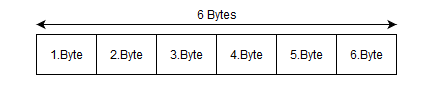
\includegraphics[width=1\linewidth]{Analyse/MACAddressOne.PNG}
	\caption{MAC-Adresse Aufbau
	\label{figure:macadresseaufbau}}
\end{figure}
Die restlichen drei Bytes sind für die Identifikation des NIC reserviert.
Es gibt zwei Bit, beide im ersten Byte der Adresse,
die für die MAC-Adresse eine besondere Relevanz haben.
Das Gruppenbit, welches sich an der letzten Stelle im Byte befindet, 
wird für die Unterscheidung von Unicast- und Multicast-Adressen verwendet.
Das Lokale oder U/L-Bit an der zweitletzten Stelle unterscheidet zwischen
global einzigartigen (und von der IEEE zugewiesenen) Adressen und lokal 
verwalteten Adressen.

\clearpage 

In der Abbildung~\ref{figure:macadressedetail} ist die Struktur der MAC-Adresse dargestellt.
\begin{figure}[h!]
	\centering
	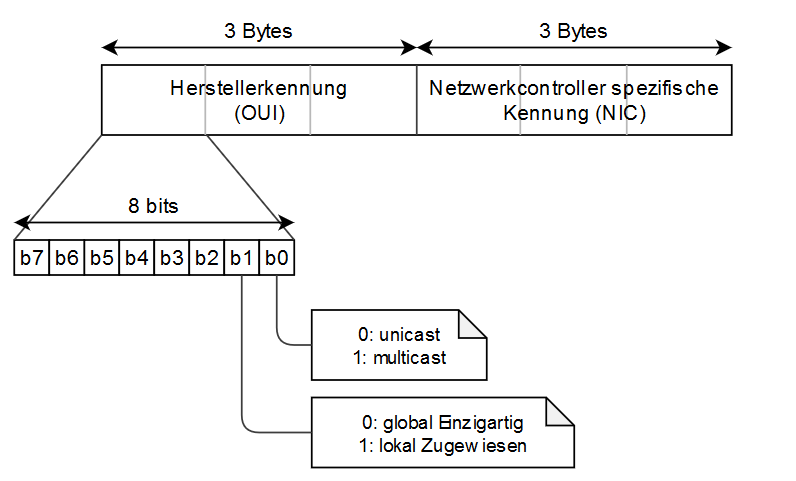
\includegraphics[width=1\linewidth]{Analyse/MACAddressTwo.PNG}
	\caption{Detaillierte MAC-Adresse
	\label{figure:macadressedetail}}
\end{figure}

Falls das lokale Bit gesetzt ist, kann dies anhand der MAC-Adresse sehr schnell
erkannt werden, da das zweite Zeichen im ersten Byte eine von vier Zahlen 
gemäss der Tabelle~\ref{table:localmacrange} ist.

\begin{table}[h!]
	\centering
	\begin{tabular}{|c|}
		\hline
		x2-xx-xx-xx-xx-xx \\
        \hline
        x6-xx-xx-xx-xx-xx \\
        \hline
        xA-xx-xx-xx-xx-xx \\
        \hline
        xE-xx-xx-xx-xx-xx \\
        \hline
    \end{tabular}
    \caption{Lokale MAC-Adressen
    \label{table:localmacrange}}  
\end{table}

\clearpage

\subsection{IEEE 802.11 WLAN Standard}
Der IEEE 802.11 Standard ist eine Ansammlung von Protokollen, 
die das Zusammenspiel von Komponenten in kabellosen Netzwerken 
(WLAN, Wireless Local Area Network) regeln, und baut auf dem 802 Standard
Für lokale Computernetzwerke (LAN) auf.

Der WLAN Standard definiert unter anderem 
auf welche Art und Weise Computer, Mobiltelefone und andere Geräte 
miteinander interagieren welche Frequenzbänder sie dabei verwenden, 
welche Formate die übertragenen Datenpakete haben müssen und welche 
Sicherheitsvorkehrungen getroffen werden sollen.

Nachfolgend wird auf die wichtigsten Spezifikationen und Konzepte eingegangen, 
die im Rahmen dieser Arbeit relevant sind.

\subsubsection*{Frequenzbänder}
Die meistverwendeten Frequenzbänder im WLAN sind das $2.4$-GHz-Band und das 
$5$-GHz-Band. Diese Frequenzbänder sind jeweils in gleich grosse Kanäle 
unterteilt.
Um Störungen durch überlappende Frequenzbänder zu verhindern, werden 
im $2.4$-GHz-Bereich in Europa üblicherweise die Kanäle $1$, $6$ und $11$ 
verwendet.
In der Abbildung~\ref{figure:lowerfrequencyband} ist die Unterteilung der 
Kanäle ersichtlich.
Im $5$-GHz-Bereich wird die Kanalunterteilung in Europa gemäss der 
Tabelle~\ref{table:higherfrequencyband} vorgenommen.

\begin{figure}[h!]
	\centering
	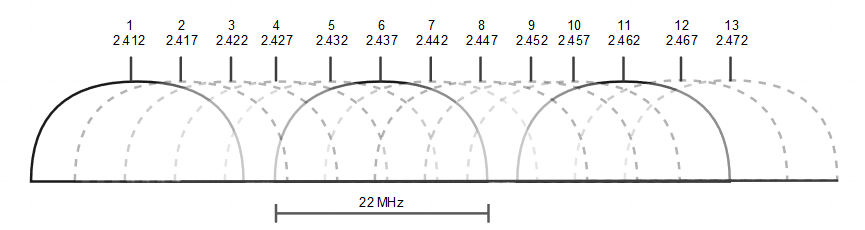
\includegraphics[width=1\linewidth]{Analyse/lowerfrequencyband.PNG}
	\caption{Kanalzuteilung im $2.4$-GHz-Frequenzband
	\label{figure:lowerfrequencyband}}
\end{figure}

\clearpage

\begin{table}[h!]
	\centering
	\begin{tabular}{|>{$}c<{$}|>{$}c<{$}||>{$}c<{$}|>{$}c<{$}|}
		\hline
        \textbf{Kanal} & \textbf{Frequenz} & \textbf{Kanal} & \textbf{Frequenz} \\
        \hline
        \phantom{0}36 & 5,180 & 108 & 5,540 \\ 	
        \phantom{0}40 & 5,200 & 112 & 5,560 \\
        \phantom{0}44 & 5,220 & 116 & 5,580 \\
        \phantom{0}48 & 5,240 &	120 & 5,600 \\
        \phantom{0}52 & 5,260 & 124 & 5,620 \\
        \phantom{0}56 & 5,280 & 128 & 5,640 \\
        \phantom{0}60 & 5,300 & 132 & 5,660 \\
        \phantom{0}64 & 5,320 & 136 & 5,680 \\
        100 & 5,500 & 140 & 5,700 \\
        104 & 5,520 & &\\	
        \hline
    \end{tabular}
    \caption{Kanalzuteilung $5$-GHz-Frequenzband. Jeder Kanal ist $20$ MHz breit. 
    \label{table:higherfrequencyband}}  
\end{table}


Geräte, die über das WLAN kommunizieren, werden auf die Kanäle aufgeteilt, 
so dass alle Kanäle gleichmässig ausgelastet sind, 
um eine möglichst grosse Datenrate für jedes Endgerät zu gewährleisten.
Somit ist es nicht möglich, nur einen Kanal zu überwachen, um sämtliche
Endgeräte in einem WLAN-Netzwerk zu identifizieren.

\clearpage

\subsection{802.11 Frames}
Im IEEE 802.11 Standard ist definiert, wie die Datenpakete, 
sogenannte Frames, aufgebaut sein müssen.
Diese Frames befinden im OSI-Modell (Siehe Abbildung~\ref{figure:ozzylayer}) 
auf dem zweiten Layer, dem Data Link Layer \\ (Sicherungsschicht).

\begin{figure}[h!]
	\centering
	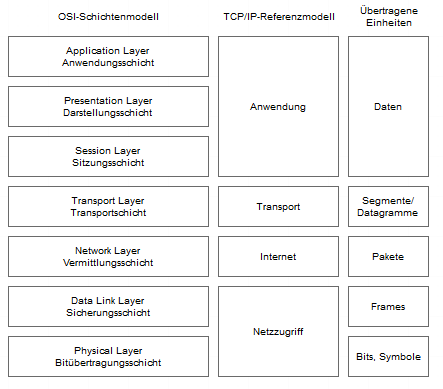
\includegraphics[width=1\linewidth]{Analyse/ozzylayer.PNG}
	\caption{OSI- und TCP/IP-Referenzmodell
	\label{figure:ozzylayer}}
\end{figure}

\clearpage

Frames können in drei Kategorien unterteilt werden:

Datenframes, welche Daten von höheren Schichten übertragen, 
z.B. TCP-Segmente aus der Transportschicht.

Control-Frames, die bei der Übertragung der Datenframes den Kontrollfluss
steuern und die Zuverlässigkeit der WLAN-Übertragung gewährleisten. \\
Beispiele für Control-Frames sind Request-To-Send- oder Acknowledgment-
Nachrichten.

Die dritte Kategorie sind die Management-Frames, welche verschiedene
Dienste auf dem Data Link Layer für WLAN anbieten, die im Kabelgebundenen
LAN nicht benötigt werden. Ein Beispiel hierfür wäre die Identifizierung von verfügbaren 
Netzwerken.
Die in dieser Arbeit untersuchten Probe-Requests gehören in diese dritte Kategorie.
In der Abbildung~\ref{figure:genericmanagementframe} ist ein Management- 
Frame dargestellt, wie es üblicherweise versendet wird. 
Die MAC-Header-Informationen sind in jedem Frame enthalten, aber die 
Information Elements können sich je nach Typ des Management-Frames unterscheiden.
Eine Erklärung der einzelnen Felder ist in der 
Tabelle~\ref{table:genericmanagementframe} angegeben.

\begin{figure}[h!]
	\centering
	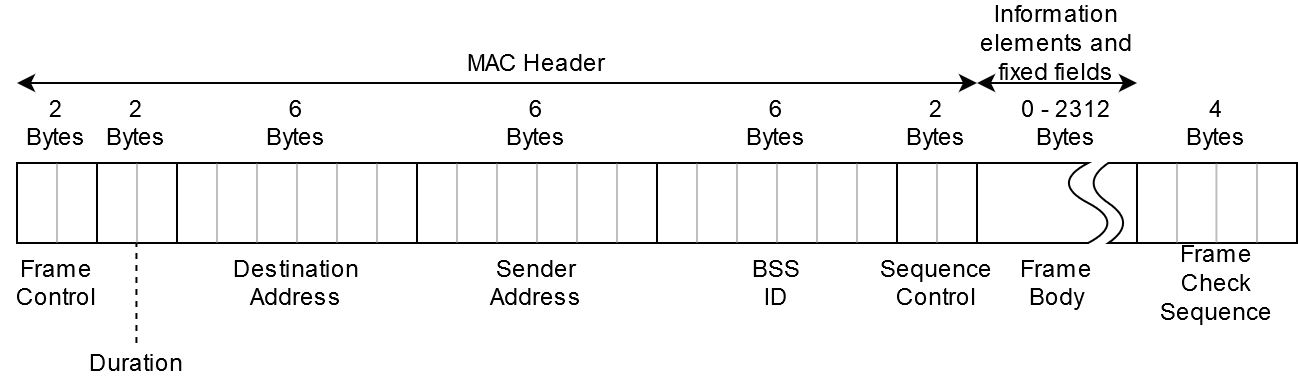
\includegraphics[width=1\linewidth]{Analyse/GenericManagementFrame.png}
	\caption{Generisches Management-Frame
	\label{figure:genericmanagementframe}}
\end{figure}

\begin{table}[h!]
	\centering
	\begin{tabular}{|c|>{$}c<{$}|l|}
		\hline
        \textbf{Feld} & \textbf{Länge} & \textbf{Bedeutung} \\
        \hline
        Frame Control & 2\, \text{Byte} & 
        Gibt die Protokollversion und Subtype- \\
        & & Informationen für das Frame an. \\
        \hline
        Duration & 2\, \text{Byte} & 
        Gibt die Zeit an, wie lange das Übertragungs- \\
        & & medium während der Übertragung des Frames \\
        & & nicht verwendet werden darf, um Kollisionen  \\
        & & zu vermeiden. \\
        \hline 
        Dest. Address & 6\, \text{Byte} & 
        MAC-Adresse des Empfängers des Frames. \\
        \hline 
        Sender Address & 6\, \text{Byte} & 
        MAC-Adresse des Sendegeräts des Frames. \\
        \hline
        BSSID & 6\, \text{Byte} & 
        BSSID steht für Basic Service Set Identifier \\
        && und beschreibt eine Zuordung verschiedener \\
        && Geräte zu einem spezifischen Netzwerk. \\
        && Üblicherweise ist die BSSID die MAC- \\
        && Adresse des Access Points \\
        \hline
        Sequence Control & 2\, \text{Byte} & 
        Dieses Feld besteht aus einer Fragmentnummer\\
        && und einer Sequenznummer. \\
        && Die Fragmentnummer beschreibt die Anzahl \\
        && Frames, die für einen Request benötigt werden. \\
        && Die Sequenznummer wird für jede Übertragung \\
        && separat festgelegt und verwendet, falls \\
        && Übertragungen wiederholt werden müssen. \\
        \hline
        Frame-Body & \text{variabel} & 
        Im Frame-Body werden die spezifischen \\
        && Informationen des jeweiligen Frames \\
        && übertragen. \\
        \hline
        Frame Check Sequence & 2\, \text{Byte} & 
        Redundanzcheck für die Validierung, dass \\
        && das Frame korrekt übertragen wurde. \\
        \hline
    \end{tabular}
    \caption{Felder in einem Management-Frame
    \label{table:genericmanagementframe}}  
\end{table}

\clearpage 

Weiterhin können Frames in drei verschiedene Klassen unterteilt werden.
Die Klassen bestimmen, welche Frames - abhängig vom Zustand des Geräts - 
überhaupt übertragen werden dürfen.
Die verschiedenen Zustände und die dazugehörigen erlaubten Klassen sind 
in der Abbildung~\ref{figure:proberequeststate} dargestellt.
Im initialen Zustand sind Geräte nicht authentifiziert und nicht einem
Access Point zugeordnet. 
Im zweiten Zustand hat sich das Gerät gegenüber dem Access Point authentifiziert,
ist aber noch nicht zugewiesen.
Im dritten Zustand ist das Gerät authentifiziert und zugewiesen.
Erst im dritten Zustand ist der Austausch von Daten erlaubt.

\begin{figure}[h!]
	\centering
	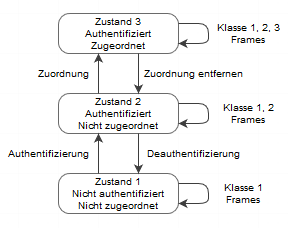
\includegraphics[width=0.8\linewidth]{Analyse/proberequeststate.PNG}
	\caption{Zustände und Klassen für Frames
	\label{figure:proberequeststate}}
\end{figure}

\clearpage

\subsection{Probe-Requests}
Probe-Requests sind Klasse-1 Management-Frames. Sie werden von End-geräten 
verwendet, um innerhalb des Sendebereiches nach WLAN-Access-Points zu suchen. 
Alternativ können Netzwerke auch gefunden werden, 
indem ausgesendete Beacon-Messages der Access Points empfangen werden.
Um sich mit einem Access Point zu verbinden, sendet ein Gerät zuerst 
Probe-Requests als Broadcast aus, um verfügbare Access Points kennen zu lernen.
Alle Access Points im Sendebereich des Geräts, die den Request erhalten,
senden eine Probe-Response, um die vom Gerät benötigten Parameter 
und die eigenen Betriebsparameter zu übermitteln. 
Das Gerät evaluiert die erhaltenen Responses, wählt für sich den 
besten Access Point aus und sendet diesem einen Auth.-Request
mit den für die Authentifizierung be-nötigten Informationen. Sind diese 
Informationen für den Access Point korrekt, sendet dieser
ein Auth.-Response und registriert das Gerät bei sich.
Das Gerät sendet daraufhin einen Association-Request welcher vom Access
Point mit einem Association-Response beantwortet wird, bevor dann der 
Austausch von Daten zwischen Endgerät und Access Point beginnt.
Der gesamte Ablauf ist in der Abbildung~\ref{figure:proberequestsequence} 
dargestellt.

\begin{figure}[h!]
	\centering
	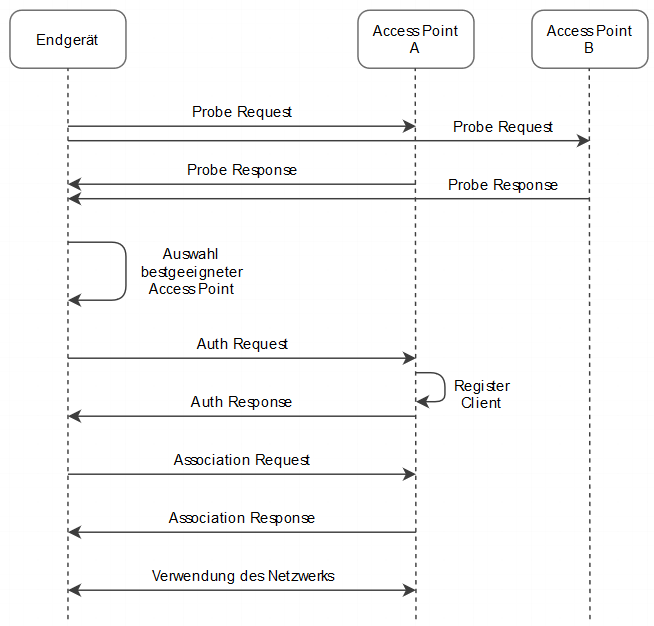
\includegraphics[width=0.8\linewidth]{Analyse/proberequestsequence.PNG}
	\caption{Sequenzdiagramm Association und Authentifizierung
	\label{figure:proberequestsequence}}
\end{figure}

Probe-Requests beinhalten alle notwendigen Informationen, die ein Access Point
benötigt, um zu entscheiden, ob er die Anforderungen des Client-Geräts 
erfüllen kann. In der Abbildung~\ref{figure:proberequestframe} ist das Frame
eines Probe-Requests ersichtlich und in der Tabelle~\ref{table:proberequestframe}
sind die einzelnen Felder erklärt.

\begin{figure}[h!]
	\centering
	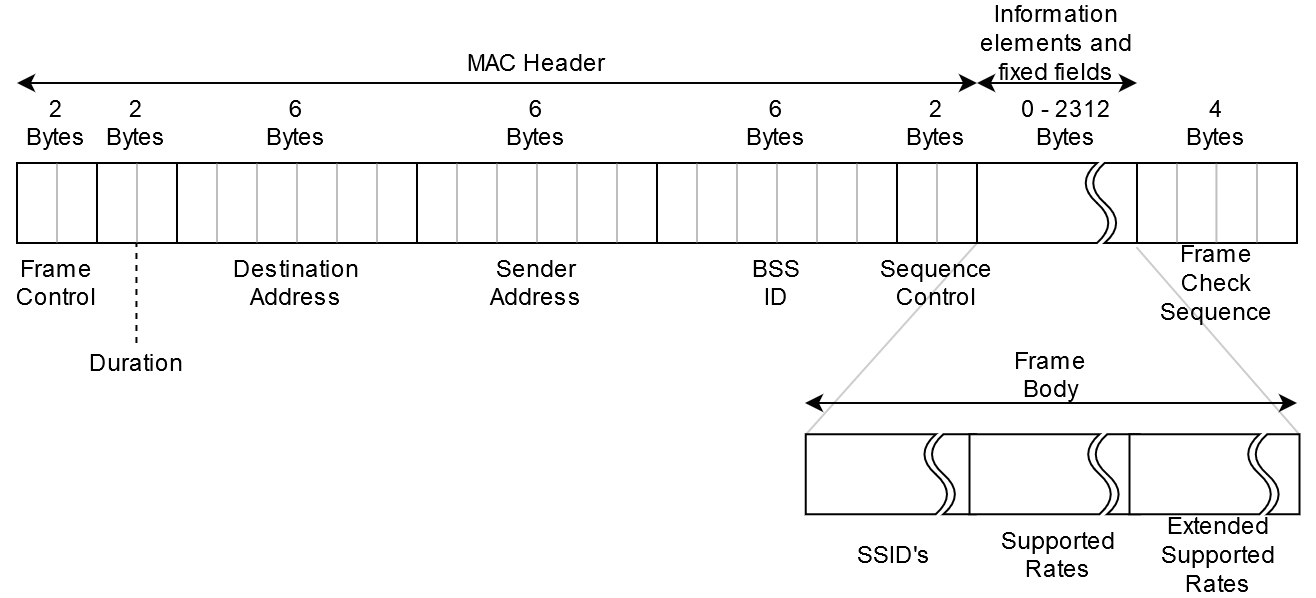
\includegraphics[width=1\linewidth]{Analyse/ProbeRequestFrame.png}
    \caption{Frame eines Probe-Requests.
	\label{figure:proberequestframe}}
\end{figure}

\begin{table}[h!]
	\centering
	\begin{tabular}{|c|c|l|}
		\hline
        \textbf{Feld} & \textbf{Länge} & \textbf{Bedeutung} \\
        \hline
        SSID & variabel & 
        Abfolge von Zeichen, um ein Netzwerk zu \\ 
        && identifizieren. \\
        && Wird manchmal auch als Netzwerkname bezeichnet. \\
        \hline
        (Extended) & variabel & 
        Datenraten, die vom Client-Gerät unterstützt werden. \\
        Supported Rates & & 
        Im IEEE 802.11 sind verschiedene Datenraten von \\
        && 1Mbit/s bis 54MBit/s standardisiert. \\
        \hline
    \end{tabular}
    \caption{Felder in einem Probe-Request
    \label{table:proberequestframe}}  
\end{table}



\clearpage

\subsection{Probe-Request-Burst}
Mobilgeräte senden Probe-Requests in Gruppen aus, welche Bursts genannt werden. 
Bursts zeichnen sich dadurch aus, dass jeder Probe-Request darin dieselbe MAC-Adresse 
verwendet. Die Anzahl Probe-Request kann dabei von Burst zu Burst variieren.
 Weiterhin sind die Sequenznummern innerhalb eines Bursts aufsteigend, 
auch wenn die Sequenznummer vom Mobilgerät zufallsgeneriert sind.
Die Information-Element-Felder der Probe-Requests  in einem Burst sind ebenfalls 
identisch.

Diese Information kann in einem Prototyp dazu verwendet werden, aufgezeichnete 
Frames in Bursts zu sortieren, bevor diese klassifiziert werden.
Da-durch müssen weniger einzelne Frames klassifiziert werden und die Effizienz eines 
Prototyps wird gesteigert, während die Fehlerrate gesenkt wird.

Die Abbildung~\ref{figure:burstcolor} zeigt eine Aufzeichnung von Probe-Requests, 
und wie deren Aufteilung in Bursts erkannt werden kann.

\begin{figure}[h!]
	\centering
	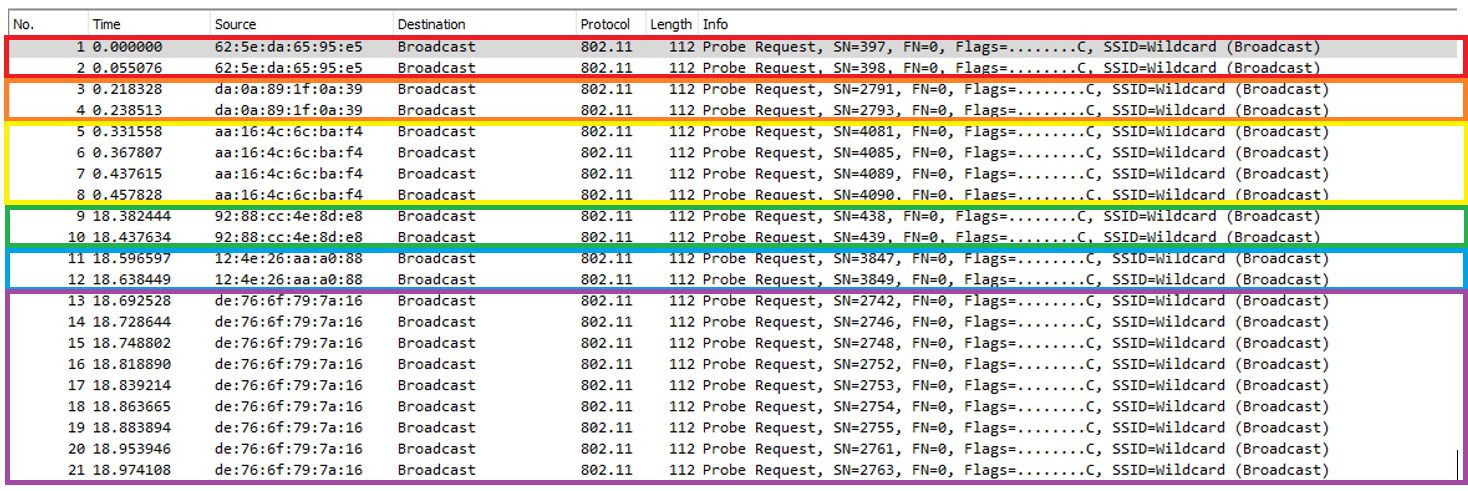
\includegraphics[width=1\linewidth]{Analyse/Burst_Explanation_with_Lines.PNG}
    \caption{Wireshark-Aufzeichnung von Probe-Requests. 
    Die Bursts sind farbig gekennzeichnet.
	\label{figure:burstcolor}}
\end{figure}

Die Probe-Requests in dieser Abbildung stammen alle vom selben Gerät. 
Man kann erkennen, dass die MAC-Adresse und Sequenznummer für jeden Burst neu 
zufallsgeneriert wird und dass die Frames alle dieselbe Länge haben, 
was bedeutet, dass sie die selben Information-Element-Felder haben.

\clearpage

\subsection{Probe-Request Header-Frame}
Der MAC-Header in einem Probe-Request hat einige für Fingerprinting 
interessante Felder. 
Bevor die MAC-Adresse zufällig gesetzt wurde, 
konnte ein Client-Gerät einfach anhand der Sendeadresse erkannt und verfolgt 
werden.
Seit einigen Android/iOS-Versionen werden diese Adressen aber zufallsgeneriert.
Die Felder, welche für ein Fingerprinting genutzt werden können, werden
nachfolgend genauer erläutert:

\subsubsection*{Frame Control} 
Das Feld enthält die in der Tabelle~\ref{table:framecontrolattributes}
beschriebenen Attribute.

\begin{table}[h!]
	\centering
	\begin{tabular}{|c|c|l|}
		\hline
        \textbf{Attribut} & \textbf{Länge} & \textbf{Bedeutung} \\
        \hline
        Protokoll & 2 bit & 
        Dieses Attribut unterscheidet verschiedene WLAN- \\
        Version && Standards. \\
        && Falls ein WLAN-2-Standard entwickelt würde, \\
        && kann dies in der Protokoll Version vom aktuellen \\
        && Standard unterschieden werden. \\
        \hline
        Type & 2 bit & 
        Das Type-Attribut unterscheidet zwischen Control-, \\
        && Daten- und Management-Frames \\
        \hline
        Subtype & 4 bit & 
        Der Subtype unterscheidet die verschiedenen Frames \\
        && zusätzlich. \\
        && Probe-Requests haben den Subtype 4 (0b0100) \\
        \hline
        To DS & 1 bit & 
        Wird gesetzt, wenn das Frame von einem Client- \\
        && Gerät zum Access Point gesandt wird. \\
        \hline
        From DS & 1 bit &
        Wird gesetzt, wenn das Frame vom Access Point zum \\
        && Client-Gerät gesandt wird. \\
        \hline 
        More & 1 bit & 
        Wird gesetzt, falls bei Datenframes die Daten in \\
        Fragments && mehreren Fragmenten übertragen werden.\\
        \hline
        Retry & 1 bit & 
        Falls ein Frame nochmals gesendet werden muss,\\
        &&  weil ein Fehler passiert ist, wird dieses Bit\\
        &&  auf 1 gesetzt. \\
        \hline 
        Power & 1 bit & 
        Akkubetriebene Geräte signalisieren mit diesem  \\
        Management &&  
        Attribut, dass sie nach dem Versenden des Frames\\
        && in den Energiesparmodus  wechseln und der\\
        && Access Point allfällige Antworten zwischen-\\
        && speichern soll. \\
        \hline
        More Data & 1 bit & 
        Falls ein Access Point Daten für ein Client-Gerät \\
        && zwischenspeichert, dann wird dieses Attribut \\
        && gesetzt, um zu indizieren, dass das Frame für \\
        && ein Gerät im Ruhemodus gedacht ist. \\
        \hline
        WEP & 1 bit & 
        Dieses Attribut indiziert, dass der Frame-Inhalt \\
        && verschlüsselt übertragen wird.\\
        \hline
        Order & 1 bit & 
        Wenn dieses Attribut gesetz ist, dann werden Frames \\
        && und dazugehörige Fragmente in der korrekten \\
        && Reihenfolge übertragen. \\
        \hline
    \end{tabular}
    \caption{Attribute im Frame-Control-Feld
    \label{table:framecontrolattributes}}  
\end{table}

In Probe-Requests sind die meisten Attribute auf 0b0 gesetzt.
Das Protokoll-Version-Attribut und der der Typ (Management) sind auch auf 
0b0 und der Subtyp auf 0b0100 (4: Probe-Request) gesetzt.

Diese Informationen können für die Filterung von aufgezeichneten Probe-Requests
verwendet werden, sind in der Unterscheidung von verschiedenen Geräten aber 
nicht relevant.

\subsubsection*{Duration}
Das Duration-Feld wird unter anderem dazu verwendet, dem Empfänger 
mitzuteilen, wie lange die Übertragung für das aktuelle Frame etwa 
dauern wird. Bei Probe-Requests beträgt die geschätzte Zeit Null Mikrosekunden.
Daher lässt sich das Duration-Feld für Fingerprinting auch nicht verwenden.

\subsubsection*{Destination Address}
Die Empfängeradresse bei Probe-Requests ist üblicherweise die Broadcast-Adresse 
(ff:ff:ff:ff:ff:ff). Auch dieses Feld lässt sich für Fingerprinting nicht 
verwenden.

\subsubsection*{Sender Address}
Die MAC-Adresse des Absenders ist, vorausgesetztd die richtigen Geräte-einstellungen
sind gesetzt, randomisiert. Es ist möglich, dass nur die NIC (Netzwerkcontroller 
spezifische Kennung) zufällig gesetzt wird, oder dass die gesamte 
MAC-Adresse randomisiert ist. Dieses Verhalten soll in der Bachelorarbeit 
ermittelt werden.

\clearpage

\subsubsection*{BSSID}
Basic Service Sets werden vergeben, um verschiedene WLAN-Netze im selben 
Gebiet untereinander zu unterscheiden.
Wie bei der Empfängeradresse wird in Probe-Requests für die BSSID auch die 
Broadcast-Adresse \\ (ff:ff:ff:ff:ff:ff) verwendet und kann für ein Fingerprinting nicht verwendet 
werden.

\subsubsection*{Sequence Control}
Das Sequence Control Feld hat zwei Attribute. 
Die Fragmentnummer wird verwendet, um Datenframes, die zu gross sind und in 
einzelne Fragmente aufgeteilt werden, in die korrekte Reihenfolge zu sortieren.
Die Sequenznummer dient der Identifikation der logischen Abfolge von Frames.
Fragmentierte oder wiederholt gesendete Frames haben die gleiche Sequenznummer. 
Die Sequenznummer würde sich für ein Fingerprinting eignen, falls sie nicht
bei neuen Probe-Requests jedes Mal zufällig gesetzt wird. 

\subsubsection*{SSID}
In Probe-Request-Frames wird das SSID Field verwendet, um ein Probe-Request zu einem
spezifischen Access Point (z.B. Eduroam) zu senden. 
Falls der Probe-Request an alle verfügbaren Netzwerke versendet wird, wird die
Broadcast-SSID, manchmal auch Wildcard-SSID genannt, verwendet.
Spezifische SSIDs können für ein Fingerprinting interessant sein.
Wenn ein Client-Gerät in verschiedenen Netzwerken Probe-Requests an dieselbe SSID
sendet, kann das Gerät, falls keine weiteren Geräte nach dieser SSID suchen,
erkannt werden. 

\subsubsection*{(Extended)-Supported-Rates}
Mit dem (Extended)-Supported-Rates Feld teilt das Client-Gerät dem Access Point
mit, welche WLAN-Datenraten unterstützt werden. 
Der Access Point entscheidet unter anderem anhand dieser Datenraten, 
ob er dem Client-Gerät einen Probe-Response senden wird.
Die unterstützten Datenraten könnten für eine Erkennung von Geräten genutzt werden.

\clearpage 

\subsubsection*{Frame Check Sequence}
Die Frame Check Sequence ist eine 32 Bit lange hexadezimale Zahl, die anhand
der im Frame gesetzten Parameter berechnet wird und eine Überprüfung der 
Frames beim Empfänger ermöglicht. Wird ein Frame empfangen, kann der Empfänger
die Frame Check Sequence über das Frame berechnen und diese mit dem im Frame
mitgelieferten Wert vergleichen. Falls die beiden Werte nicht übereinstimmen,
wird das Frame verworfen, oder allenfalls neu angefordert.
Die Frame Check Sequence lässt sich nicht für ein Fingerprinting verwenden.

\subsubsection*{Weitere Information-Element-Felder}
Es ist möglich, dass neben den vorgehend erwähnten Feldern im Frame, 
welche alle vorhanden sein müssen, noch optionale Information-Element-Felder
übermittelt werden, um weitere Funktionalitäten abzudecken oder weitere
Eigenschaften des Client Geräts zu übermitteln.
Diese IE-Felder sind für das Fingerprinting wahrscheinlich die interessanteste
Quelle von Informationen, wenn diese sich von Mobilgerät zu Mobilgerät 
tatsächlich unterscheiden.

\clearpage

\section{Verwandte Arbeiten}
Es gibt duzende Papers zum Thema Fingerprinting auf Mobilgeräten.
Die relevantesten vier Arbeiten wurden in den folgenden Unterabschnitten
in der Reihenfolge ihrer Publikation zusammengefasst.

Es gilt zu erwähnen, dass in diesem Abschnitt Informationen aus den Papers
direkt übersetzt und übernommen wurde. 

\subsection{How Talkative is Your Mobile Device?}
\begin{itemize}
    \item Name: How Talkative is your Mobile Device? An Experimental Study of Wi-Fi 
    Probe-Requests
    \item Autoren: Julien Freudinger
    \item Publikationsjahr: 2015
\end{itemize}
Das Paper beschäftigt sich mit der Frage, welche Informationen von einem
Mobilgerät über Probe-Requests versendet werden.
Die wichtigsten Erkenntnisse sind eine Evaluation für den experimentellen
Versuchsaufbau, um Probe-Requests zu sniffen, die Messresultate aus den 
durchgeführten Messungen und eine Evaluation eines kommerziell genutzten 
MAC-Address-\\ Randomization-Algorithmus.

\subsubsection*{Experimenteller Versuchsaufbau und Resultate}
Die Experimente, welche im Paper beschrieben werden, 
beschreiben acht unterschiedliche Konfigurationen für die Messeinrichtung und
weitere acht für die Mobilgeräte und die aus den Messungen gewonnenen Resultate.
Für die Messungen wurden ein Samsung S3 mit Android 4.4.2, 
ein iPhone 6 mit IOS 8.1.3 und ein Nexus 5 mit Android L 5.0.1 verwendet.

\clearpage 

Die Konfigurationen für die Messeinrichtung sind nachfolgend aufgelistet.
Die Kanäle 1, 6 und 11 werden nachfolgend als reservierte Kanäle bezeichnet.
\begin{itemize}
    \item 1.dynamic: Eine Antenne, welche über die drei reservierten 2.4-GHz-Kanäle misst.
    \item 1.static: Drei Mess-Konfigurationen, jeweils statisch auf einem separaten reservierten 
    2.4-GHz-Kanal.
    \item 3.dynamic: Drei Antennen, die koordiniert über die reservierten 2.4-GHz-Kanäle 
    messen. (Die Antennen springen in regelmässigen Abständen auf den nächsten Kanal und 
    sind jeweils um einen Kanal verschoben)
    \item 3.dynamic.s: Drei Antennen, die über die reservierten 2.4-GHz-Kanäle messen.
    (Jede Antenne springt frei über die reservierten Kanäle.)
    \item 3.dynamic.sn: Drei Antennen die über die reservierten 2.4-GHz-Kanäle und die 
    in der Tabelle~\ref{table:higherfrequencyband} erwähnten 5-GHz-Kanäle messen.
    \item 3.static: Pro reserviertem Kanal wird jeweils eine Antenne statisch eingestellt.
\end{itemize}

Die Messungen wurden jeweils eine Stunde lang durchgeführt und fünfmal 
wiederholt.
Als Ergebnisse wurden die durchschnittlich aufgezeichnete Anzahl der Probe-
Requests und eine Schätzung der nicht aufgezeichneten Requests gespeichert.
Die nicht aufgezeichneten Probe-Requests können aus den Sequenznummern 
abgeschätzt werden. Werden in einer Messung beispielsweise drei Probe-Requests mit den
Sequenznummern 1, 3 und 5 aufgezeichnet, kann davon ausgegangen werden,
dass zwei Probes mit den Sequenznummern 2 und 4 nicht aufgezeichnet wurden.

Die Verwendung von mehreren Antennen ist ein Ansatz, welcher in anderen Arbeiten
z.T. nicht beachtet wurde und dazu führen kann, dass nur ca. $57$ Prozent der Probe
Requests tatsächlich gemessen und in den Ergebnissen berücksichtigt wurden.

\clearpage

Die Konfiguration der Mobilgeräte ist nachfolgend aufgelistet:
\begin{itemize}
    \item Default: Das Mobilgerät ist gesperrt, an ein Ladekabel angeschlossen,
    nicht mit einem WLAN verbunden und Bluetooth ist ausgeschaltet. Das Gerät
    kennt vier Netzwerke.
    \item Not Charging: Das Mobilgerät ist nicht an ein Ladekabel angeschlossen.
    \item Screen ON: Das Gerät wird alle fünf Minuten entsperrt und wieder gesperrt.
    \item Wi-Fi Connected: Das Gerät ist mit einem WLAN verbunden.
    \item Wi-Fi Settings ON: Das Mobilgerät befindet sich im Menu für die Auswahl 
    des WLANs, es wird aber sonst nicht mit dem Gerät interagiert.
    \item Bluetooth ON: Bluetooth ist während den Messungen eingeschaltet.
    \item Airplane ON: Der Flugmodus ist während den Messungen eingestellt und
    das WLAN auf dem Mobilgerät eingeschaltet.
    \item Known In Proximity: Ein dem Gerät bekanntes WLAN erscheint alle fünf
    Minuten für 10 Sekunden im Empfangsbereich des Mobilgeräts.
\end{itemize}
Die Resultate zeigen, dass wenn die WLAN-Einstellungen eingeschaltet werden 
oder wenn der Bildschirm aktiviert wird, die Anzahl ausgesendeter
Probe-Requests ansteigt. 
Eine Ausnahme ist hierbei das Nexus 5, welches keinen signifikanten Unterschied
bei den ausgesendeten Probes aufweist.

Weiterhin wurde gemessen, welche Auswirkung die Anzahl bekannter Netzwerke 
auf einem Mobilgerät auf die Anzahl ausgesendeter Probe-Requests hat.
Das iPhone sendet erst ab 20 bekannten SSIDs eine erhöhte Anzahl von Probes aus.
Auf dem Nexus werden unabhängig von den bekannten Netzwerken immer etwa gleich
viel Probe-Requests ausgesandt.
Lediglich das Samsung S3 versendet mit steigender Anzahl bekannter Netzwerke
eine erhöhte Anzahl Probes.

Im Paper wird jeweils davon ausgegangen, dass diese aufgezeichneten 
Geräte-verhalten vom Betriebssystem abhängen. 
Es wurden keine Messungen mit unterschiedlichen Geräten mit demselben
Betriebssystem vorgenommen, um den Einfluss von Hardware auf das Probing-
Verhalten zu untersuchen.

\clearpage

\subsubsection*{MAC-Address-Randomization-Algorithmus}
In den durchgeführten Messungen werden verschleierte MAC-Adressen des iPhones
untersucht und festgestellt, dass die Sequenznummern im iOS 8 nicht zufällig
initialisiert werden, sondern aufsteigend vorkommen.
Ausserdem wird in iOS 8 die MAC-Adresse nur dann verschleiert, wenn das Gerät 
im Ruhemodus ist. 
Das bedeutet, dass iPhones mit iOS 8 relativ einfach identifiziert werden können,
wenn man die nicht randomisierte MAC-Adresse aufzeichnet und die 
Sequenznummern mit denjenigen Probe-Requests vergleicht, die eine verschleierte
MAC-Adresse haben. Hat man beispielsweise in Wireshark einen Probe mit der 
MAC `Apple\_12:84:05' und der Sequenznummer `1337' und einen Probe-Request 
mit der MAC `52:61:6E:64:6F:6D' und der Sequenznummer `1340', kann man davon 
ausgehen, dass die beiden Probe-Requests vom selben Gerät ausgesendet wurden.

Weiterhin senden Mobilgeräte mit iOS 8 oder Android 4 und 5 in den Information-
Element-Feldern herstellerspezifische Informationen mit, welche es zusätzlich
vereinfachen, Probe-Requests mit verschleierten MAC-Adressen zu einem spezifischen
Gerät zuzuordnen.

\clearpage

\subsection{Defeating MAC Address Randomization Through Timing Attacks}
\begin{itemize}
    \item Name: Defeating MAC Address Randomization Through Timing Attacks
    \item Autoren: Célestin Matte et al.
    \item Publikationsjahr: 2016
\end{itemize}
In diesem Paper wird ein Verfahren erarbeitet, mit dem die Verschleierung
von MAC-Adressen mittels eines Timing-Angriffs neutralisiert wird.
Es wird davon ausgegangen, dass die verschiedenen Betriebssysteme dahingehend
angepasst wurden, dass die Mobilgeräte keine identifizierenden Informationen 
mehr aussenden und nur das Timing der Probe-Requests für ein möchliches 
Fingerprinting verwendet werden kann.
Dabei wird vorausgesetzt, dass die Frames, die von Geräten ausgesendet
werden, einem Muster folgen, welches sich für eine Identifikation nutzen lässt.

MAC-Adressen werden in vielen Implementationen nach einigen Probe-Requests 
neu randomisiert. 
Eine Gruppe von Probe-Requests, die in einem Zeitfenster von ungefähr zehn
Millisekunden ausgesandt werden, wird auch Burst genannt.
Ausserdem ist in der Praxis die tatsächliche Anzahl Mobilgeräte im Empfangsbereich
eines WLAN-Access-Points nicht bekannt.
Die Schwierigkeit eines solchen Ansatzes besteht darin, mit einer sehr geringen Menge 
von Informationen ein zuverlässiges Fingerprinting durchführen zu können, 
ohne dass zuvor eine Datensammlung möglich gewesen ist. 
Die Autoren beschreiben als Lösung für diese Problematik die Verwendung 
inkrementeller Lernmethoden für die Clusterbildung unter der Verwendung
einer handelsüblicher Netzwerkkarte, die nur einen Kanal gleichzeitig \\
überwachen kann.

\subsubsection*{Zeitbasierte Signatur}
Probe-Requests lassen sich gruppieren, indem die Inter-Frame-Arrival-Time
(Zwischenankunftszeit, nachfolgend IFAT genannt) der einzelnen Frames mit 
der selben MAC-Adresse analysiert wird.
Der Algorithmus~\ref{algorithm:timeattack} beschreibt in Pseudocode, 
wie ein Identifikator zu einem Frame hinzugefügt werden kann.

\clearpage

\begin{algorithm}
    \KwIn{
        \\
        $G$: groups of burdst sets, grouped by MAC
        \\
        $t$: distance threshold 
        \\
        $d$: a distance function
    }
    \KwResult{$A$: dictionary of aliases}
    \BlankLine
    $A \longleftarrow \emptyset $\;
    $D \longleftarrow \emptyset $\tcp*[r]{Database of signatures}
    \ForEach{$B \in G$}{
        $S \longleftarrow $signature($B$)\;
        $d_{\text{min}} \longleftarrow min(d(S,S')\, \text{where}\, S' \in D)$\;
        \If{$d_{\text{min}} < t$}{
            $A[B.mac] \longleftarrow A[S'.mac]$\;
        }\Else{
            $A[B.mac] \longleftarrow B.mac$\;
        }
        $D \longleftarrow D \cup S$
    }
    \Return{$A$}
    \caption{Algorithmus für die identifikation von MAC-Frames
    \label{algorithm:timeattack}}
\end{algorithm}

Der Algorithmus hat als Input ein beliebiges Capture-File mit gemessenen
Probe-Requests und liefert als Output ein Mapping von Identifikatoren und
den Frames. 
Für alle Frames mit der selben MAC-Adresse wird die IFAT, 
die Auftretenswahrscheinlichkeit und der Durchschnitt der IFAT berechnet.
Anhand dieser Berechnungen wird basierend auf der eingegebenen Distanzgrenze
(distance threshold) entschieden, ob zwei Signaturen zum selben Gerät gehören.

Im Paper werden drei Distanzmass-Algorithmen genannt, 
auf die hier nicht weiter eingegangen wird. 
Bei Interesse des Lesers empfiehlt sich das Studium des Papers.
Weiterhin wird der Algorithmus an einem Datenset von 120'000 Proberequests
validiert und hat eine Erfolgsquote von ungefähr $77,2$ Prozent.

\clearpage 

\subsection{Why MAC Address Randomization is not Enough}
\begin{itemize}
    \item Name: Why MAC Address Randomization is not Enough: 
    An Analysis of Wi-Fi Network Discovery Mechanisms
    \item Autoren: Mathy Vanhoef et al.
    \item Publikationsjahr: 2016
\end{itemize}

In der Recherche zum Thema Mobile Fingerprinting taucht dieses Paper in 
sehr vielen anderen Quellen als Referenz auf. 
Darin wird eine fundierte Analyse diverser Methoden für die Deanonymisierung
von Mobilgeräten vorgenommen und erwiesen, dass die Verschleierung von 
MAC-Adressen allein keine Garantie für die Privatsphäre der Nutzer ist.

Der Hauptansatz besteht in der Analyse von Information-Element-Feldern
und den Sequenznummern, um Mobilgeräte voneinander zu unterscheiden.
Insgesamt werden zwölf IE-Felder genannt, die für ein Fingerprinting 
relevant sein können und nachfolgend aufgelistet sind.
\begin{itemize}
    \item HT capabilities info 
    \item Ordered list of tags numbers 
    \item Extended capabilities
    \item HT A-MPDU parameters 
    \item HT MCS set bitmask
    \item Supported rates 
    \item Interworking access net. type
    \item Extended supported rates 
    \item WPS UUID 
    \item HT extended capabilities
    \item HT TxBeam Forming Cap. 
    \item HT Antenna Selection Cap.
\end{itemize}
Weiterhin könnte die Reihenfolge der IE-Tags eine weitere Informationsquelle 
für ein mögliches Fingerprinting sein.

\clearpage

Auch in diesem Paper wird ein Algorithmus beschrieben, 
welcher ein Fingerprinting auf Mobilgeräte ermöglicht.

\begin{algorithm}
    \KwIn{
        \\
        $P$: List of captured probe requests
        \\
        $\Delta T$: maximum time between two probes 
        \\
        $\Delta S$: maximum sequence number distance 
    }
    \KwResult{Set of clusters corresponding to devices}
    \BlankLine
    $M \longleftarrow \emptyset$\tcp*[r]{$M$ maps fingerprints to clusters}
    \ForAll{$p \in P$}{
        $f \longleftarrow \text{fingerprint}(p) $\tcp*[r]{Calculate IE fingerprint}
        $M[f].\text{append}(p) $\tcp*[r]{Append probe to cluster}
    }
    $ D \longleftarrow []$\tcp*[r]{List of clusters representing devices}
    \ForAll{$C \in M$}{
        $S \longleftarrow [] $\tcp*[r]{Will contain subdivision of C}
        $m \longleftarrow \text{max}(p.seq\, \mathbf{for}\, p\, \mathbf{in}\, C) $\;
        \ForAll{$p \in C$}{
            $\text{Find}\, i\, \text{such that:} $\tcp*[f]{Fing matching cluster}\\
            $\qquad \text{d}(S[i].last.seq,\, p.seq,\, m) \leq \Delta S$\;
            $\qquad \text{and}\, p.time - S[i].last.time \leq \Delta T$\; 
            \If{$no\, i\, found$}{
            $i \longleftarrow |S|$\tcp*[r]{Create new subcluster}
        }
        $S[i].append(p)$\tcp*[r]{Add p to subcluster}
        }
        $D.extend(S)$\tcp*[r]{Extend list D with S}
    }
    \Return{$D$}
    \caption{Gruppierungsalgorithmus basierend auf IE-Feldern
    \label{algorithm:ieattack}}
\end{algorithm}
    
Der Algorithmus berechnet zuerst für alle Probe-Requests einen Fingerprint
anhand der IE-Felder und weist diesen einem Cluster zu. 
Die Cluster werden basierend auf den Sequenznummern in Gruppen unterteilt.

Da in modernen Betriebssystemen die Sequenznummer auch zufällig gesetzt wird,
kann das Clustering nicht mehr anhand der Sequenznummer durchgeführt werden.
In einem eigenen Prototypen müsste für die Clusterbildung eine eigene
Methodik entworfen werden.

\clearpage

\subsection{Noncooperative 802.11 MAC Layer Fingerprinting}
\begin{itemize}
    \item Name: Noncooperative 802.11 MAC Layer Fingerprinting and Tracking
    of Mobile Devices
    \item Autoren: Pieter Robyns et al.
    \item Publikationsjahr: 2017
\end{itemize}

In diesem Paper wird eine pro-Bit-Entropie Analyse von Probe-Request-Frames
durchgeführt und eine Technik vorgestellt, die mittels eines Fingerprints 
und zeitlichen Daten ein Gerät mit bis zu $80$ Prozent Genauigkeit erkennen und 
verfolgen kann, ohne dass dafür spezielle Hardware benötigt wird.

\subsubsection*{Identifikatoren und Fingerprinting}
Es wird zwischen zwei Typen von Identifikatoren unterschieden.
Explizite Identifikatoren, zu denen eine MAC-Adresse gehört, erlauben es,
ein Gerät eindeutig zu identifizieren.
Implizite Identifikatoren sind Informationen, die nicht absichtlich für 
die Identifikation gedacht sind, aber sich von Gerät zu Gerät genügend 
unterscheiden, um damit ein Fingerprinting durchzu-führen.
Unter der Annahme, dass die MAC-Adresse in Mobilgeräten anonymi-siert wird,
müssen für ein Fingerprinting die impliziten Identifikatoren verwendet werden.

\subsubsection*{Bitweise MAC-Header-Analyse}
In weiteren Arbeiten wird oftmals ein spezifisches Element des MAC-Headers
für ein Fingerprinting verwendet und das restliche Frame verworfen.
Dieses Paper schlägt vor, anhand der Entropie der einzelnen Header-Felder
automatisch zu evaluieren, welche Informationen für ein Fingerprinting 
verwendet werden sollen.
Dabei wird davon ausgegangen, dass das Mobilgerät jedes Frame einzeln
anonymisiert und nicht mit einem Access Point assoziiert ist. 
Das bedeutet, die vorgeschlagene Technik ist für die Anwendung auf 
ein einzelnes Frame ausgelegt.

Im Paper werden drei wichtige Metriken vorgestellt:
\begin{itemize}
    \item Bit-Variabilität: Einzelne Bits unterscheiden sich von Gerät zu
    Gerät dahingehend, dass sie sich für ein Fingerprinting eignen.
    \item Bit-Stabilität: Für ein Gerät bleiben die Bits, 
    die sich zu anderen Geräten unterscheiden, in nacheinander auftretenden
    Frames soweit stabil, dass sie weiterhin für einen Fingerprint 
    verwendet werden können.
    \item Bit-Verwendbarkeit: Die Verwendbarkeit ist eine Kombination der
    Variabilität und der Stabilität und sagt aus, ob das Bit für ein 
    Fingerprinting tatsächlich verwendet wird.
\end{itemize}

\clearpage

\subsubsection*{Berechnung der Variabilität}
Die Variabilität ist die Entropie eines Bits gemessen über mehrere Frames
welche jeweils von einem anderen Mobilgerät ausgesendet werden.
Dabei wird pro Gerät nur ein einzelnes Frame in Betracht gezogen, 
um keinen Bias in das System einzufügen.

Um die Entropie eines Bits an der Position $i$ in einem Frame zu berechnen,
wird zuerst die diskrete Wahrscheinlichkeitsdichte ($P(X_{i})$) für 
jeden Bitwert an der Position $i$ berechnet.
$X_{i}$ ist dabei die Zufallsvariable, welche einen Bitwert repräsentiert.
Somit ist $X_{i} \in \{0, 1, U\}$, wobei $U$ bedeutet, dass das Bit nicht 
vorhanden ist.
Die Wahrscheinlichkeitsdichte kann dann verwendet werden, um die 
Shannon-Entropie zu berechnen, wie in der 
Formel~\ref{equation:shannonentropy} dargestellt.

\begin{equation}
    \label{equation:shannonentropy}
    H(X_{i}) = - \sum_{x \in \{0, 1, U\}} P(X_{ix}) \log_{3} P(X_{ix})
\end{equation}

Da für die Berechnung der Entropie ein Bit mit drei möglichen Zuständen
(Wert 1 oder 0 und nicht vorhanden) beschrieben wird, wird der $\log_{3}$
anstatt dem üblichen $\log_{2}$ verwendet.
$H(X_{i})$ hat nun einen Wert zwischen $0$ und $1$, wobei $0$ bedeutet, 
dass keine Entropie vorhanden ist und $1$ bedeutet, dass eine maximale 
Entropie vorhanden ist.
Das Resultat kann als Vektor $\vec{v}$ repräsentiert werden:

\begin{equation}
    \vec{v} = [H_{1}\; H_{2}\; \cdots H_{n-1}\; H_{n}]
\end{equation}

Hierbei ist $n$ die Anzahl der Bits im Frame und $H_{n}$ die Entropie des 
jeweiligen Bits ist.

\subsubsection*{Berechnung der Stabilität}
Die Stabilität eines Bits wird als $1$ minus die Entropie dieses Bits, 
gemessen über mehrere Frames von einem Gerät, definiert.
Der Wert sagt aus, wie hoch die Wahrscheinlichkeit ist, dass das 
Bit über mehrere Übertragungen gleich bleibt.
Der Nutzen der Stabilität ist, dass diejenigen Bits, die sich pro Gerät
häufig verändern, im Fingerprinting nicht berücksichtigt werden.
Die Formel~\ref{equation:stability} zeigt den Resultierenden 
Stabilitätsvektor $\vec{s_{d}}$ pro Mobilgerät $d$:

\begin{equation}
    \label{equation:stability}
    \vec{s_{d}} = [1-H_{d1}\; 1-H_{d2}\; \cdots 1-H_{dn-1}\; 1-H_{dn}]
\end{equation}

\clearpage

Im Gegensatz zur Variabilität bedeutet ein hoher Wert bei der Entropie,
dass die Stabilität geringer wird. 
Darum wird die Stabilität mit $1-H(X_{i})$ berechnet.
Da die Stabilität pro Gerät berechnet wird, muss der Vektor $\vec{s}$
durch eine Mittelwertsberechnung der Werte des Vektors $\vec{s_{d}}$
berechnet werden, um diesen für die weiteren Operationen verwenden zu können.

\subsubsection*{Berechnung der Verwendbarkeit}
Im Idealfall sind Variabilität und Stabilität beide genügend hoch, 
um damit ein Fingerprinting durchführen zu können. 
Um die Verwendbarkeit - darge-stellt durch den Vektor $\vec{u}$ - zu berechnen,
werden im Paper zwei Ansätze vorgestellt, die beide in der Praxis anwendbar
sind. 

Der erste Ansatz ist ein statistisches Vorgehen, welches die Variabilität
und Stabilität als Wahrscheinlichkeit betrachtet, da beide im Wertebereich
$[0, 1]$ sind. Davon ausgehend, dass $\vec{v} \text{ und } \vec{s}$ 
voneinander unabhängige Variablen sind, kann die Verwendbarkeit mit der
Formel
\begin{equation}
    \vec{u} = \vec{v} \odot \vec{s}
\end{equation}
berechnet werden.

Der zweite Ansatz geht davon aus, dass die Stabilität zu bevorzugen ist
und deshalb in der Berechnung nur die Variabilität verwendet wird.
Diejenigen Bits, deren Stabilität unter einem gewissen Schwellwert $\lambda$ 
liegen, werden aus der Berechnung ausgeschlossen.

\begin{equation}
    \vec{u_{i}} = 
    \begin{cases}
        \vec{v_{i}},\quad \text{if}\; \vec{s_{i}} \geq \lambda, \\
        0,\quad \text{otherwise}
    \end{cases}
\end{equation}

Falls beispielsweise der Schwellwert $\lambda = 1$ gesetzt wird, 
wird dadurch sichergestellt, dass kombinierte Bits im Fingerprint über die 
Zeit immer stabil bleiben.

Da die IE-Felder nicht unbedingt in allen Probe-Requests in der gleichen 
Reihenfolge vorkommen, müssen die Variabilität und Stabilität für 
die IE-Felder unabhängig ihrer Reihenfolge berechnet werden.

\clearpage
\cleardoublepage

\section{Allgemeine Mobilgeräte-Analyse}
\label{analyse}
Bevor in der Bachelorarbeit damit begonnen werden konnte, Auswertungen über 
Mobilgeräte vorzunehmen, musste die allgemeine Verteilung von Smartphones
auf dem Schweizer Mark analysiert werden. 
Dafür wurden Zahlen vom Bundesamt für Statistik aus dem Jahr 2019 ausgewertet
und ergänzend Verkaufszahlen und Nutzerstatistiken bekannter Hersteller gesucht.

\subsection{Smartphones}
In der Schweiz gibt es im Jahr $2020$ ungefähr $6.8$ Millionen Personen,
die ein Smartphone besitzen.
Prognosen sagen aus, dass bis im Jahr $2025$ über $7$ Millionen Personen
ein Mobilgerät besitzen werden. 
In der Abbildung~\ref{figure:AnzSmartphoneUser} sind die statistischen
Zahlen und Prognosen bis zum Jahr $2022$ ersichtlich.    

\begin{figure}[h!]
    \centering
    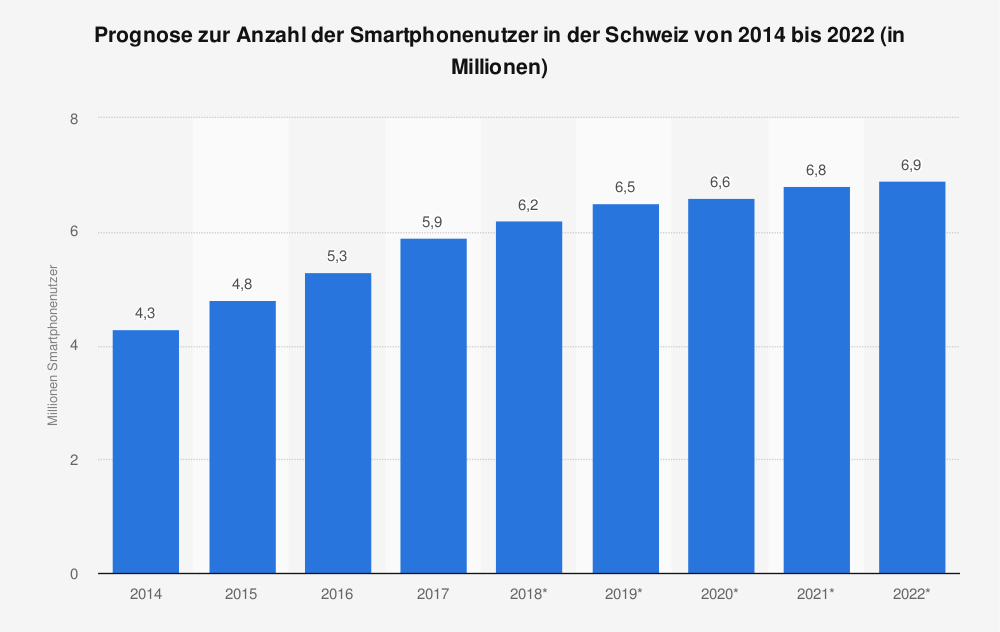
\includegraphics[width=1\linewidth]{Analyse/anz_smartphone_nutzer_prognose.png}
    \caption{Anzahl Smartphone User in der Schweiz}
    \label{figure:AnzSmartphoneUser}
\end{figure}

\clearpage
    
Um die Nutzung der Mobilgeräte noch weiter zu unterteilen, wurde eine 
Aufteilung nach Betriebssystem der Smartphones durchgeführt.
Die Ergebnisse sind in der Abbildung~\ref{figure:SmartphoneBsys} aufgezeigt.

\begin{figure}[h!]
    \centering
    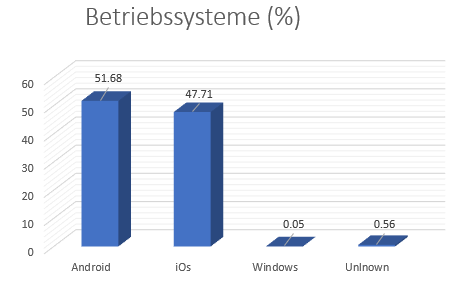
\includegraphics[width=1\linewidth]{Analyse/smartphone_bsys.PNG}
    \caption{Verteilung der Betriebssysteme}
    \label{figure:SmartphoneBsys}
\end{figure}

Hauptsächlich sind die beiden Betriebssysteme Android und IOS mit zusammen
über $99$ Prozent Marktanteil im Jahr $2019$ vertreten.

\clearpage

IOS wird nur von IPhones verwendet, aber Android-Geräte lassen sich noch weiter
nach Hersteller unterteilen. 

In der Abbildung~\ref{figure:SmartphoneHersteller} ist die Verteilung
nach Hersteller im Jahr $2019$ aufgelistet.

\begin{figure}[h!]
    \centering
    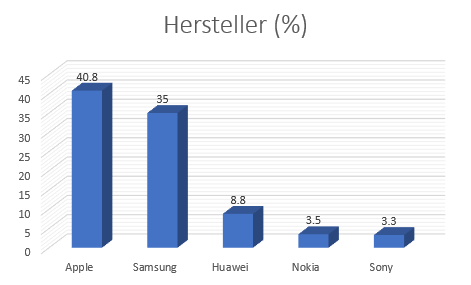
\includegraphics[width=1\linewidth]{Analyse/smartphone_hersteller.PNG}
    \caption{Verteilung der Hersteller}
    \label{figure:SmartphoneHersteller}
\end{figure}

Die meistverwendeten Smartphones sind entweder IPhones oder Samsung-Geräte.
Huawei hat mit $8.8$ Prozent einen eher kleinen Marktanteil und wird in naher Zukunft
ein eigenes Betriebssystem für seine Geräte anbieten, da der Hersteller 
aufgrund diverser Privatsphäreanschuldigungen in der USA auf schwarzen Liste 
steht. 

\clearpage

\subsection{Auswahl der Mobilgeräte}
Basierend auf den gewonnenen Erkenntnissen konnten die für die Versuche
benötigten Mobilgeräte ausgewählt werden.

In der Analyse der beiden Betriebssysteme IOS 
(Siehe Abschnitt~\ref{section:iosanalysis}) und Android
(Siehe Abschnitt~\ref{section:androidanalysis}) hat sich gezeigt, dass
IOS-Geräte ab IPhone 8 und Android-Geräte mit der Android-Version 9 oder neuer
für die Versuche in Betracht gezogen werden. 
Nachfolgend sind die Geräte aufgelistet.

\paragraph{IOS-Geräte}
\begin{itemize}
    \item IPhone 8
    \item IPhone X
    \item IPhone XR
    \item IPhone XS
    \item IPhone 11
    \item IPhone 11 Pro
    \item IPhone SE
\end{itemize}

\paragraph{Samsung-Geräte}
\begin{itemize}
    \item Samsung Galaxy S8
    \item Samsung Galaxy S9
    \item Samsung Galaxy S9+
    \item Samsung Galaxy S10
    \item Samsung Galaxy S10 light
    \item Samsung Galaxy S20
    \item Samsung Galaxy S20+
    \item Samsung Galaxy S20 ultra
\end{itemize}

\paragraph{Google-Geräte}
\begin{itemize}
    \item Pixel 3
    \item Pixel 3 XL
    \item Pixel 3a
    \item Pixel 3a XL
    \item Pixel 4
    \item Pixel 4 XL
\end{itemize}

\paragraph{Weitere Hersteller}
\begin{itemize}
    \item OnePlus 7T 
    \item Oneplus 7T Pro 
    \item Oneplus 8
    \item Oneplus 8 Pro
    \item Huawei P20
    \item Huawei P30
    \item Fairphone 3
    \item Fairphone 3+
    \item Weitere, falls Android-Version 9 oder neuer
\end{itemize}

Die Auflistung zeigt nur die Geräte, welche für die Versuche in 
Betracht gezogen werden. Die tatsächlich verwendeten Geräte 
werden im Kapitel~\ref{chapter:experiments}: Versuche aufgelistet.

\clearpage
\cleardoublepage

\section{IOS-Analyse
\label{section:iosanalysis}}
Apple verwendet MAC-Adress-Randomisierung seit der IOS Version 8, 
welche am 17. September 2014 veröffentlicht wurde.
Die Einführung von Randomisierung wurde nich nur als Absicht aufgefasst,
die Privatsphäre der Apple-Benutzer besser zu schützen. 
Es wurde spekuliert, dass Apple die eigene Positionierungstechnologie
IBeacon vorantreiben möchte, ein Service, der es erlaubt, IOS-Geräte 
zu lokalisieren und Pushnachrichten oder personalisierte Werbung auf diesen 
Geräten zu schalten.

In den folgenden Untersektionen werden die verschiedenen IOS-Versionen ab der
Version 8 analysiert und aufgezeigt, wie sich die Verschleierung von 
MAC-Adressen weiterentwickelt hat.
Es gilt noch zu erwähnen, dass Apple keine Dokumentationen für diese Features
herausgibt und sämtliche Informationen über verschiedene Quellen zusammengesucht 
werden müssen.
Eine Auflistung der Versionsgeschichte findet sich in der 
Tabelle~\ref{table:iosversionhistory}.

\subsection{Versionsgeschichte}
\begin{table}[H]
    \begin{tabularx}{\linewidth}{XXX}
        \toprule 
        \textbf{Aktuellste Version} & \textbf{Erscheinungsdatum} & \textbf{Letzte Version für} \\
        \midrule
        3.1.3 & 02.02.2010 & IPhone 2G \\
        4.2.1 & 22.11.2010 & IPhone 3G \\
        5.1.1 & 07.05.2012 & - \\
        6.1.6 & 21.02.2014 & IPhone 3GS \\
        7.1.2 & 30.06.2014 & IPhone 4 \\
        \rowcolor{lightgray}
        8.4.1 & 13.08.2015 & - \\
        \rowcolor{lightgray}
        9.3.5 & 25.08.2016 & - \\
        \rowcolor{lightgray}
        9.3.6 & 22.07.2019 & IPhone 4S \\
        \rowcolor{lightgray}
        10.3.3 & 19.07.2017 & IPhone 5C \\
        \rowcolor{lightgray}
        10.3.4 & 22.07.2019 & IPhone 5 \\
        \rowcolor{lightgray}
        12.4.7 & 20.05.2020 & IPhone 5S, IPhone 6 \\
        \rowcolor{lightgray}
        13.7 & 01.09.2020 & - \\
        \rowcolor{lightgray}
        14 & 16.09.2020 & - \\
        \bottomrule 
    \end{tabularx}
    \caption{Versionsgeschichte des iOS für iPhones, 
    alle grau eingefärbten Zeilen benutzen MAC Randomisierung
    \label{table:iosversionhistory}}
\end{table}

\subsection{iOS 8}
Das iOS 8 wurde am 2. Juni 2014 vorgestellt, am 14. September 2014
eingeführt und von den Geräten IPhone 4 bis 6 verwendet. 
Die Version 8 ist die erste, die bei IPhones bei Probe-Requests die 
MAC-Adresse randomisiert.
Die offizielle Ankündigung auf der Apple-Webseite ist in der 
Abbildung~\ref{figure:MACRandAnnoucement} ersichtlich.

\begin{figure}[h!]
    \centering
    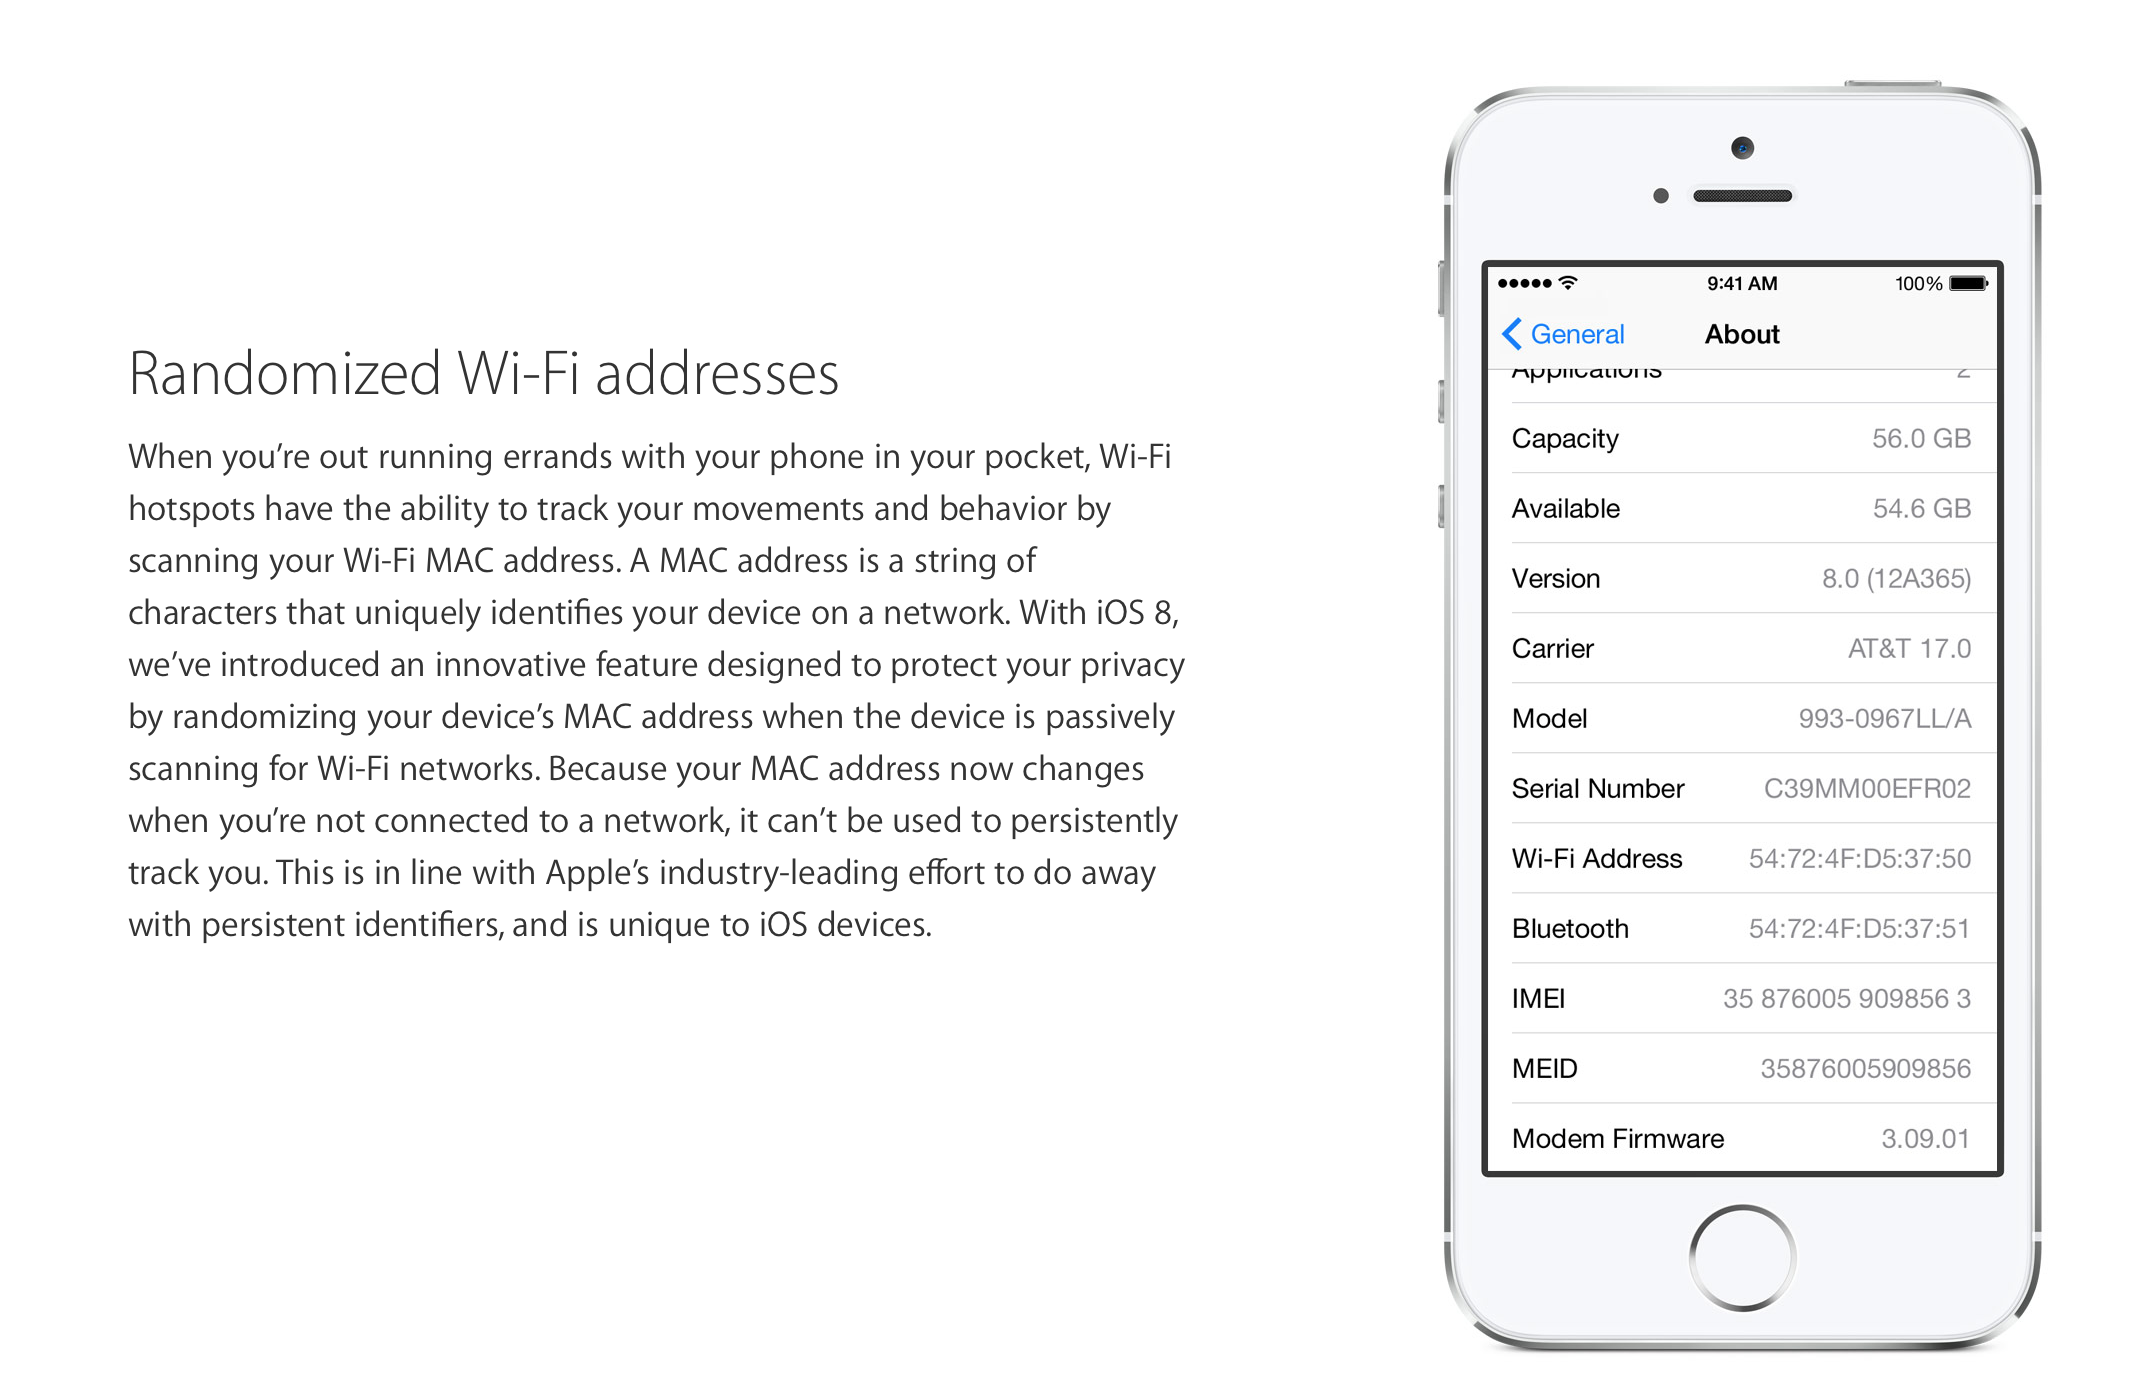
\includegraphics[width=1\linewidth]{Analyse/iOS8_rand_announcement.png}
    \caption{Offizielle Randomisierungs-Ankündigung von Apple}
    \label{figure:MACRandAnnoucement}
\end{figure}

Allerdings wird die Randomisierung nur dann ausgeführt, wenn die folgenden
drei Bedingungen erfüllt sind.

\begin{itemize}
    \item Das Wifi muss aktiviert sein, das Gerät darf aber nicht mit einem Hotspot assoziert sein.
    \item Das Smartphone muss sich im Sleep Mode befinden.
    \item Der Location Service muss in den privacy Settings explizit ausgeschaltet sein.
\end{itemize}

\clearpage

Somit wird die Randomisierung nur dann verwendet, wenn der Benutzer sich nicht
bereits mit einem Netzwerk verbunden hat, das Gerät gerade nicht verwendet und
explizit die Location Services ausgeschaltet hat.
Viele Applikationen diese Location Services aber voraus und 
die meisten Nutzer machen sich nicht den Aufwand, jedes Mal die Einstellungen
anzupassen, wenn sie eine Applikation verwenden wollen. 
Diese Faktoren haben dazu geführt, dass iOS-Geräte die MAC-Adresse häufig nicht 
zufallsgeneriert haben, obwohl Hard- und Software dies ermöglicht hätten.

\subsection{iOS 9}
Nachdem die Implementation der Randomisierung in der iOS Version 8 kritisiert
wurde, wurde das Verfahren in der Version 9 überarbeitet und verbessert.
In der Tabelle~\ref{table:iosversionninediff} ist der direkte Vergleich 
von iOS 8 zu iOS 9 ersichtlich.

\begin{table}[H]
    \begin{tabularx}{\linewidth}{|X|r|r|}
        \hline
            & \textbf{iOS 8} & \textbf{iOS 9} \\
        \hline
        Unassociated PNO Scans & Yes & Yes \\
        Unassociated ePNO Scans & Yes & Yes \\
        Location Scans & No & Yes \\
        Auto Join Scans & No & Yes \\
        \hline 
    \end{tabularx}
    \caption{Abdeckung der verschiedenen Scans in iOS 8 \& 9
    \label{table:iosversionninediff}}
\end{table}

Jeder dieser vier Scans wird in Form eines Probe-Requests versendet und der einzige
Unterschied besteht darin, unter welchen Bedingungen diese Requests versendet werden.
PNO und ePNO sind (enhanced) Preferred Network Offload Scans, die verwendet werden,
um nach bekannten Netzwerken zu suchen, während sich das Gerät im Ruhemodus befindet.
Location Scans werden von Applikationen verwendet, welche die Positionierung des 
Geräts erkennen möchten, wie beispielsweise eine Navigations-Applikation.
Auto Join Scans sind Probe-Requests für bekannte Netzwerke wie Starbucks oder 
Eduroam.

\clearpage

\subsection{iOS 10 - 13}
Es wurden in der Recherche keine Informationen gefunden, ob und wie die MAC-Address-
Randomisierung weiterentwickelt wurde. 
In der offiziellen Apple Platform Security Dokumentation wird erwähnt, dass
ab dem iPhone 7 in Probe-Requests zusätzlich zur Randomisierung der MAC-Adresse 
auch die Sequenznummer zufallsgeneriert wird. 
Es wird nicht angegeben, welche iOS Version das Feature implementiert, aber 
anhand der unterstützten Geräte (iPhone, iPad, MacBooks etc.) lässt sich schliessen,
dass die Sequenzverschleierung frühestens ab iOS 11 eingeführt wurde.

\subsection{iOS 14}
IOS 14 wurde am 22. Juni 2020 vorgestellt und am 16.09.2020 veröffentlicht.
Mit der neuen Software-Version wurden auch diverse Änderungen vorgestellt, 
auf welche Art die MAC-Randomisierung vorgenommen wird und wie der User Einfluss
auf die Privatssphäreeinstellungen nehmen kann.

In der neuen Version verwendet ein iPhone für jedes Wi-Fi Netzwerk eine eigene
randomisierte MAC-Adresse um sich mit dem Netzwerk zu verbinden. 
Zusätzlich wird die MAC alle 24 Stunden geändert, damit die eigentliche 
MAC-Adresse des iPhone dem Access Point niemals bekannt gegeben wird.

Die Verschleierung von MAC-Adressen ist in iOS 14 standardmässig aktiviert und
die User haben mehr Möglichkeiten, die Privatssphäreeinstellungen ihren eigenen
Bedürfnissen anzupassen.

Allerdings gibt es auch Kritik an den neuen Praktiken von Apple.
Wenn ein Mobilgerät sich nur über komplett Randomisierte MAC-Adressen mit 
Netzwerken verbinden, können dadurch Probleme auftreten, da für viele 
Betreiber von Access Points die MAC-Adresse eine Form der Authentifizierung ist.

Weiterhin ist zu erwähnen, dass iOS 14 erst gerade auf den Markt gebracht wurde und
in vergangenen Versionen mit minor Releases immer neue Funktionen und Verhalten
hinzugefügt wurden. 
Somit ist es gut möglich, dass in der Version 14.1 die MAC-Address-Randomisierung
bereits komplett anders gehandhabt wird.
\cleardoublepage

\section{Android-Analyse
\label{section:androidanalysis}}
Android implementierte erstmals mit Android 6 (Marshmallow) Support für Developer
für die Verschleierung von MAC-Adressen in Probe-Requests.

In Versuchen im Paper "A Study of MAC Adress Randomization in Mobile Devices 
and when it Fails" von Jeremy Martin et. al. aus dem Jahr 2017 wird beschrieben, 
dass die meisten Geräte mit Android 6 die Randomisierung der MAC-Adresse auf Hardwareebene 
gar nicht unterstützen da die Chipsets nicht dazu in der Lage waren.

Erst ab Android 8 (Oreo) wurde die Randomisierung der MAC-Adressen bei Probe-Requests
von Android Geräten offiziell als Funktion implementiert (zuvor war die Option nur 
für Developer verfügbar) und standardmäßig verwendet.

Die Versionsgeschichte des Android Betriebssystem ist in der 
Tabelle~\ref{table:androidversionhistory} ersichtlich.

\subsection{Versionsgeschichte}
    \begin{table}[H]
        \begin{tabularx}{\linewidth}{XXXXX}
            \toprule 
            \textbf{Name} & \textbf{Nummer} & \textbf{Erscheinung} & \textbf{Supported} & \textbf{API Lvl} \\
            \midrule
            Honeycomb & 3.0 - 3.2.6 & 22.02.2011 & No & 11 - 13 \\
            Icecream Sandwich & 4.0 - 4.0.4 & 18.102011 & No & 14 - 15 \\
            Jelly Bean & 4.1 - 4.3.1 & 09.07.2012 & No & 16 - 18 \\
            KitKat & 4.4 - 4.4.4 & 31.10.2013 & No & 19 - 20 \\
            \rowcolor{lightgray}
            Lollipop & 5.0 - 5.1.1 & 12.11.2014 & No & 21 - 22 \\
            \rowcolor{lightgray}
            Marshmallow & 6.0 - 6.0.1 & 05.10.2015 & No & 23 \\
            \rowcolor{lightgray}
            Nougat & 7.0 - 7.1.2 & 22.08.2016 & No & 24 - 25 \\
            \rowcolor{lightgray}
            Oreo & 8.0 - 8.1 & 28.08.2017 & Yes & 26 - 27 \\
            \rowcolor{lightgray}
            Pie & 9 & 06.08.2018 & Yes & 28 \\
            \rowcolor{lightgray}
            Android 10 & 10 & 03.09.2019 & Yes & 29 \\
            \rowcolor{lightgray}
            Android 11 & 11 & 08.09.2020 & Yes & 30 \\
            \bottomrule 
        \end{tabularx}
        \caption{Versionsgeschichte des Android, 
        alle grau eingefärbten Zeilen benutzen MAC-Randomisierung.
        Supported Devices erhalten noch aktuelle Sicherheitsuptades
        \label{table:androidversionhistory}}
    \end{table}

    \clearpage

\subsection{Android 8 - Oreo}
Ab Android 8.0 verwenden Android-Geräte bei der Suche nach Wi-Fi Netzwerken
zufällige MAC-Adressen in Probe-Requests.
Für jeden Scan wird eine neue zufällige Adresse generiert und zusätzlich
wird die Sequenznummer zufällig generiert.

\subsection{Android 9 - Pie}
Mit Android 9.0 wurde die Developer-Option hinzugefügt,
für jede Verbindung mit einem Wi-Fi-Netzwerk eine zufällige MAC-Adresse zu verwenden.

\subsection{Android 10}
Die Verwendung von zufälligen MAC-Adressen für jedes Netzwerk wurde in Android 10 
standardmäßig aktiviert. 

\subsection{Android 11}
In Android 11 Beta 1 wurde die Option "Wi-Fi enhanced MAC Randomization" hinzugefügt.
Wenn der Access Point dies erlaubt, bzw. wenn auf dem Access Point die MAC-Randomisierung
aktiviert ist, dann wird jedes Mal, wenn sich das Gerät mit diesem Access Point verbindet,
eine neue MAC-Adresse generiert.

\clearpage

\part{Versuche
\label{chapter:experiments}}
\section{Einleitung}
Um das Verhalten von Mobilgeräten aufzuzeichnen, muss ein Versuchsumfeld 
geschaffen werden, welches erlaubt, die Geräte unter möglichst realitätsnahen 
Bedingungen zu messen.
Weiterhin soll das Versuchsumfeld verhindern, dass Störfaktoren die Messergebnisse 
beeinflussen.

Die beiden Anforderungen Wirklichkeitstreue und Störfaktorfreiheit schliessen
sich zum Teil gegenseitig aus.
Zum einen kann in einem isolierten Messraum nicht das selbe Umfeld simuliert 
werden, welches ein Mobilgerät im täglichen Gebrauch antrifft.
Zum anderen können Probe-Requests von anderen Geräten die Messergebnisse 
erheblich verfälschen, vor allem wenn diese Probe-Requests mit anonymisierten
MAC-Adressen durchgeführt werden und das zu messende Gerät nicht von den 
störenden Geräten unterschieden werden kann.

Es wurde entschieden, die Messungen in einem Faraday-Käfig 
durchzuführen, damit Fremdgeräte nicht die Versuche beeinflussen.
Das Institut für Kommunikationstechnik ICOM hat eine Antennenmesskammer 
für die Messungen von Antennen und Kommunikationssystemen.
Diese Messkammer kann Signale von ausserhalb des Messraums genügend abschirmen,
dass diese nicht die Elektronik im Messraum beeinflussen.
Nach einer kurzen Recherche wurde an Marcel Kluser verwiesen, 
der den Gebrauch der Messkammer für die Dauer der Experimente bewilligt hat.

\subsection{Versuchsaufbau}
Die Messkammer besteht aus einem Innenraum mit $1.5m$ x $2.5m$ Grundfläche, 
ist ca. $2m$ hoch und in der Kammer mit Schaumstoffspitzen ausgekleidet, 
welche die Signalausbreitung aus der Kammer eindämmen. 
Die Aussenhülle besteht aus Metall und kann durch eine Türe den Innenraum
komplett von der Aussenwelt abschotten.

In der Messkammer sind jeweils folgende Geräte im Betrieb:
\begin{itemize}
    \item Das zu messende Mobilgerät
    \item Ein Laptop mit Wireshark im Monitormodus oder ein WLAN-Messgerät, 
    angeschlossen an einen Laptop.
    \item Ein weiteres Mobilgerät für die Simulation eines WLAN-Access-Points.
\end{itemize}

Die Abbildung~\ref{figure:experimentalsetup} zeigt den Versuchsaufbau mit 
den verwendeten Geräten.

\begin{figure}[h!]
	\centering
	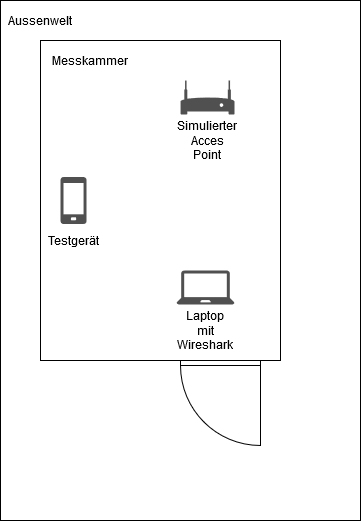
\includegraphics[width=1\linewidth]{Experiments/Messaufbau.png}
    \caption{Messaufbau in der Antennenmesskammer.
	\label{figure:experimentalsetup}}
\end{figure}

\clearpage

\subsection{Verwendete Tools}
Für die Versuchsdurchführung wurde ein Macbook verwendet, welches über eine 
Netzwerkkarte verfügt, die das Messen von Probe-Requests ermöglicht.
Auf dem Macbook ist Wireshark installiert, ein Netzwerk-Protokoll-Analyse-tool
welches die Analyse von Computersignalen verschiedener Protokolle erlaubt.
Der Monitormodus in Wireshark wird verwendet, um WLAN-Kommunikation im 
Empfangsbereich des Macbooks aufzuzeichnen.
Solange das Macbook Wireshark im Monitormodus betreibt, werden keine eigenen
Probe-Requests ausgesendet.
Weiterhin wurde ein WaveXpert WLAN-Messgerät verwendet, 
welches über einen Laptop betrieben wird und auf mehreren Kanälen gleichzeitig
Wireless-Kommunikation aufzeichnen kann.
Bei der Verwendung des WaveXpert werden die Probe-Request des Betriebslaptops
mit aufgezeichnet und müssen bei der Auswertung der Messergebnisse durch 
Filterregeln im Wireshark entfernt werden. 

Mit Wireshark aufgezeichnete Messungen werden als .pcapng-Dateien gespeichert,
welche mit Wireshark wieder geöffnet und analysiert werden können.
Es ist möglich, die Messungen in diversen Formaten zu exportieren, 
wobei das JSON-Format die ursprünglichen Informationen der Messung am 
besten erhält und Informationen in einer hierarchischen Struktur speichert,
die es erlaubt, die Messdaten einfach weiter zu verarbeiten.

Es wurde ein Python-Skript geschrieben, welches die Messdaten aus dem 
JSON-Format extrahiert und in ein Excel einträgt. 
Excel wurde für die Analyse ausgewählt, da in Excel sehr schnell einfache
Auswertungen durchgeführt werden können. 
Für die Weiterverarbeitung in einem Prototyp können die Daten in ein dafür
geeignetes Format codiert werden indem das Skript angepasst wird.

Um einen Access Point zu simulieren, wird ein weiteres Mobilgerät verwendet, 
welches in den dafür vorgesehenen Messungen einen Hotspot generiert.
Während den Messungen, die keinen Hotspot benötigen, befindet sich das
Mobilgerät im Flugmodus, um selbst keine Probe-Requests auszusenden.
Als zusätzliche Sicherheit wurde die Randomisierung von MAC-Adressen auf 
dem Mobilgerät ausgeschaltet, damit fälschlich ausgesendete Probes einfach
durch Filter entfernt werden können.

Die zu testenden Mobilgeräte werden in den jeweiligen 
Unterabschnitten genauer beschrieben.

\clearpage

\subsection{Durchzuführende Messungen
\label{subsection:plannedexperiments}}
Um das Verhalten der Mobilgeräte in verschiedenen Situationen aufzuzeichnen,
wurden diverse Tests spezifiziert.

Da die Mobilgeräte gemäss der Recherchen ein unterschiedliches Verhalten haben,
je nachdem ob sie in Gebrauch oder im Ruhemodus sind, werden die Tests in beiden
Zuständen durchgeführt.

Es soll gemessen werden, ob Geräte Probes aussenden, wenn die Wireless-
Einstellung ausgeschaltet ist. 
Da es möglich ist, dass dieses Verhalten in den Einstellungen angepasst werden
kann, müssen die Messungen jeweils mit den Einstellungen ein- und ausgeschaltet
durchgeführt werden (falls vorhanden).

Falls die Verschleierung der MAC-Adressen eine Einstellung auf dem Gerät ist,
soll jeweils für beide Einstellungen eine Messung durchgeführt werden.

Da in früheren Arbeiten die Anzahl bekannter Access Points auf dem Mobilgerät
die Anzahl ausgesandter Probe-Request beeinflusst hat, sollen alle Messungen
mit unterschiedlicher Anzahl bekannter SSID's durchgeführt werden.

Damit das Probing-Verhalten eines Mobilgeräts während dem Einschalt-vorgang und
beim Wechsel in den bzw. aus dem Flugmodus aufgezeichnet werden kann, 
werden Messungen durchgeführt, während das Mobilgerät respektive der 
Flugmodus abwechslungsweise ein- und ausgeschaltet wird.

Weiterhin soll untersucht werden, ob Mobilgeräte, die mit einem Access Point
verbunden sind, weiterhin Probe-Requests aussenden und ob in diesen Frames 
die MAC-Adresse verschleiert ist.

Für den Betrieb im Ruhemodus, im aktiven Modus und mit verbundenem WLAN 
ist jeweils zusätzlich eine Langzeitmessung von einer Stunde vorgesehen, 
um genügend Frames aufzuzeichnen, dass ein mögliches Pattern in der 
Randomisierung der MAC-Adresse oder der Sequenznummer erkannt werden kann.
Die anderen Messungen sind auf ein Zeitfenster von zehn Minuten begrenzt, wobei
bei den Messungen mit ausgeschaltetem WLAN der Versuch abgebrochen wird, falls 
nach einer Minute keine Probe-Requests aufgezeichnet werden.

Gesamthaft werden pro Mobilgerät neun Stunden lang Messungen durchgeführt, 
wobei zwei Stunden und 40 Minuten eingespart werden können, wenn mit 
ausgeschaltetem WLAN keine Probe-Requests ausgesendet werden.

Zusätzlich sollen Messungen mit mehreren Mobilgeräten im Empfangsbereich
durchgeführt werden, um realistische Messdaten zu erhalten. 
Mit diesen Messungen kann ein  Prototyp während der Entwicklung verifiziert 
werden.  

\clearpage

\subsection{Erwartete Messergebnisse}
In der Recherche hat sich herausgestellt, dass moderne Betriebssysteme von 
Mobilgeräten die MAC-Adresse für sämtliche Probe-Requests randomisieren sollten, 
solange sie nicht mit einem Access Point assoziiert sind. 
Weiterhin sollten die Sequenznummern auch zufällig für jede Gruppe von 
Probe-Requests neu gesetzt werden.
Es wird davon ausgegangen, dass die herstellerspezifischen Felder in den Frames
der Probes nicht mitgesendet werden und die IE-Felder zwischen den Probe-
Requests von unterschiedlichen Geräten mehrheitlich identisch sind.

Die einzigen zwei Möglichkeiten, den Geräten einen Fingerprint zuzuweisen,
sehen die Autoren in der Reihenfolge und Anzahl der IE-Felder oder über einen 
Timing-basierten Ansatz.

\subsection{Messplan}
Die Tabellen~\ref{table:experimentalplanone} und~\ref{table:experimentalplantwo} 
zeigen die Messplanung, welche für die Versuche in der Messkammer verwendet 
wurde.

\begin{table}[h!]
	\centering
	\begin{tabular}{|c|c|c|c|c|}
		\hline
        \textbf{Testbeschreibung} & \textbf{WiFi} & \textbf{Privacy-Settings} & \textbf{Zeit}  \\
        \hline
        Messung im Startup & Ein & Ein & 10 min  \\
        Mit WLAN verbunden & Ein & Ein & 10 min  \\
        Suche nach versteckter SSID & Ein & Ein & 10 min \\
        Messung im Flugmodus & Ein & Ein & 10 min \\
        \hline
        Langzeitmessung Ruhemodus & Ein & Ein & 60 min \\
        Langzeitmessung Aktivmodus & Ein & Ein & 60 min \\
        Langzeitmessung Verbunden & Ein & Ein & 60 min \\
        \hline
    \end{tabular}
    \caption{Messplan: SSID-unabhängige Messungen
    \label{table:experimentalplanone}}  
\end{table}

\begin{table}[h!]
	\centering
	\begin{tabular}{|c|c|c|c|c|c|}
		\hline
        \textbf{Testbeschreibung} & \textbf{WiFi} & \textbf{Privacy-Settings} & \textbf{Zeit} & \textbf{Bekannte SSID's} \\
        \hline
        Gerät im Ruhemodus & Ein & Ein & 10 min & 10 \\
        & Ein & Aus & 10 min & \\
        & Aus & Ein & 10 min & \\
        & Aus & Aus & 10 min & \\ 
        Gerät aktiv & Ein & Ein & 10 min & \\
        & Ein & Aus & 10 min & \\
        & Aus & Ein & 10 min & \\
        & Aus & Aus & 10 min & \\ 
        \hline 
        Gerät im Ruhemodus & Ein & Ein & 10 min & 5 \\
        & Ein & Aus & 10 min & \\
        & Aus & Ein & 10 min & \\
        & Aus & Aus & 10 min & \\ 
        Gerät aktiv & Ein & Ein & 10 min & \\
        & Ein & Aus & 10 min & \\
        & Aus & Ein & 10 min & \\
        & Aus & Aus & 10 min & \\
        \hline 
        Gerät im Ruhemodus & Ein & Ein & 10 min & 1 \\
        & Ein & Aus & 10 min & \\
        & Aus & Ein & 10 min & \\
        & Aus & Aus & 10 min & \\ 
        Gerät aktiv & Ein & Ein & 10 min & \\
        & Ein & Aus & 10 min & \\
        & Aus & Ein & 10 min & \\
        & Aus & Aus & 10 min & \\  
        \hline 
        Gerät im Ruhemodus & Ein & Ein & 10 min & 0 \\
        & Ein & Aus & 10 min & \\
        & Aus & Ein & 10 min & \\
        & Aus & Aus & 10 min & \\ 
        Gerät aktiv & Ein & Ein & 10 min & \\
        & Ein & Aus & 10 min & \\
        & Aus & Ein & 10 min & \\
        & Aus & Aus & 10 min & \\ 
        \hline
    \end{tabular}
    \caption{Messplan: SSID-abhängige Messungen
    \label{table:experimentalplantwo}}  
\end{table}

\clearpage

\subsection{Beschaffung der Geräte}
Um an Mobilgeräte für die Messungen zu kommen, wurden verschiedene mögliche 
Quellen angefragt.
Das Institut für Softwareentwicklung IFS unterhält mehrere Mobilgeräte für 
Test-, Entwicklungs- und Ausstellungszwecke, die für die Versuche ausgeliehen
werden durften.
Weiterhin wurde im Freundes- und Familienkreis nachgefragt, 
ob moderne Mobilgeräte mit den zu messenden Betriebssystemversionen 
verwendet werden und ob diese ausgeliehen werden dürfen.
Es hat sich herausgestellt, dass iPhones im persönlichen Umfeld weniger in 
Gebrauch sind als Android-Geräte.
Dies stellt allerdings kein grösseres Problem dar, 
da Android auf einem breiteren Spektrum von Hardware verwendet wird, 
die potentiell grösseren hardwarespezifische Abweichungen im Verhalten aufweisen können.

Welche Mobilgeräte tatsächlich für die Messungen verwendet wurde, 
wird in den jeweiligen Abschnitten beschrieben.

\clearpage
\section{IOS-Messungen
\label{section:iosmeasurements}}
Nachfolgend sind die Messungen auf Mobilgeräten mit iOS-Betriebssystem
und daraus gewonnene Erkenntnisse beschrieben.

Gesamthaft wurden 38 Einzelmessungen in 13 Stunden und 20 Minuten durchgeführt.

\subsection{Versuchsdurchführung}
Die im Unterabschnitt~\ref{subsection:plannedexperiments} genannten Messungen
wurden auf insgesamt drei iPhones durchgeführt, welche in der Tabelle 
~\ref{table:measurediosdevices} aufgeführt werden. 

\begin{table}[h!]
	\centering
	\begin{tabular}{|c|c|c|}
		\hline
        \textbf{iPhone Typ} & \textbf{iOS-Version} & \textbf{Besitzer} \\
        \hline
        iPhone 8 & 14.0.1 & Pascale Meier \\
        iPhone X & 14.0.1 & Raphael Jud \\
        iPhone X & 12.3.1 \& 14.0.1 & IFS \\
        \hline
    \end{tabular}
    \caption{Gemessene iOS-Geräte
    \label{table:measurediosdevices}}  
\end{table}

Die zwei Messungen mit dem iPhone X vom IFS und die Messung mit dem iPhone 8 konnten 
komplett durchgeführt werden. 
Das iPhone X von Raphael Jud stand uns nur für fünf Stunden zur Verfügung und wir mussten uns
auf die wichtigsten Messungen beschränken. 
Dazu haben wir uns entschieden, die Langzeitmessungen zu bevorzugen, 
da in diesen Messungen das Verschleiern der MAC-Adressen besser nachvollzogen 
werden kann. 
Weiterhin haben wir uns entschieden, dass im Bedarfsfall die nicht 
durchgeführten Messungen mit dem iPhone X von Raphael Jud zu einem späteren Zeitpunkt 
nachgeholt werden müssen.

Zusätzlich ist uns aufgefallen, dass die Anzahl der bekannten SSID's in iPhones 
vom Gerät selbst verwaltet wird und wir keinen Zugriff auf die bekannten 
Netzwerke haben und diese nicht beeinflussen können.
Eine kurze Internetrecherche hat ergeben, dass ohne Applikationen von 
Drittherstellern diese Einstellung nicht vorgenommen werden kann.
Es gibt weiterhin die Möglichkeit, die Netzwerkeinstellungen auf dem jeweiligen
iPhone über die Geräteeinstellungen zu löschen.
Beide Optionen konnten auf dem iPhone X von Raphael Jud und dem iPhone 8 nicht durchgeführt
werden, da beides Leihgeräte sind und wir keine Geräteeinstellungen verändern
wollen, die sich nicht rückgängig machen lassen.
Somit mussten wir die Messungen mit unterschiedlichen bekannten SSID's 
auch aus der Versuchsdurchführung streichen.

\clearpage 

Eine weitere Einstellung, die auf Android-Geräten vorgenommen werden kann, auf 
iPhones aber nicht existiert, sind die Privacy Settings.
Auf Andriodgeräten kann in den Lokalitätseinstellungen bestimmt werden, 
ob das Gerät Probe-Requests aussendet, obwohl das WLAN ausgeschaltet ist.
IOS erlaubt nur das ein- und ausschalten der Standorteinstellung.
Wir haben den Messplan dahingehend angepasst, dass die Messungen mit iOS jeweils
mit dem Standort anstatt der Privatsphäreeinstellung durchgeführt werden.

\subsection{Ergebnisse}
Mit den im vorherigen Unterabschnitt genannten Einschränkungen konnten die 
folgenden Messergebnisse produziert werden. 

\subsubsection*{Probe-Requests}
In der Tabelle~\ref{table:iosproberesults} ist ersichtlich, wie viele 
Probe-Requests pro Messung aufgezeichnet wurden, wie viele davon in Bursts 
gruppiert waren, die minimale, durchschnittliche und maximale Burstgrösse 
sowie eine Schätzung der nicht aufgezeichneten Frames und die durchschnittliche 
Zwischenankunftszeit zwischen zwei Bursts.

\begin{landscape}
    \begin{table}[h!]
	    \centering
        \begin{tabular}{|c|c|c|c|c|c|c|c|c|}
            \hline
            \textbf{iPhone} & \textbf{iOS Version} & \textbf{Anzahl} & \textbf{Anzahl} & \textbf{min.} & \textbf{avg.} & \textbf{max.} & \textbf{Verpasste} & \textbf{Zwischen-}\\
             & & \textbf{Probes} & \textbf{Bursts} & \textbf{Burstgrösse} & \textbf{Burstgrösse} & \textbf{Burstgrösse} & \textbf{Frames} & \textbf{ankunftszeit}\\
            \hline
            iPhone 8 & iOS 14.0.1 & 1219 & \phantom{0}327 & 1 & 4.372 & 26 & 1196 & 67.02 s \\
            \hline 
            iPhone X - R.J. & iOS 14.0.1 & 1070 & \phantom{0}309 & 1 & 3.849 & 12 & 2382 & 58.27 s \\
            \hline 
            iPhone X - IFS & iOS 12.3.1 & \phantom{0}762 & \phantom{0}193 & 1 & 4.051 & 12 & 1809 & 48.51 s \\
            \hline
            iPhone X - IFS & iOS 14.0.1 & 1784 & \phantom{0}400 & 1 & 4.609 & 18 & 2320 & 36.03 s \\
            \hline
            TOTAL & & 4835 & 1229 & 1 & 4.220 & 26 & 7707 & 52.46 s \\
            \hline
        \end{tabular}
        \caption{Ergebnisse der iOS-Messungen
        \label{table:iosproberesults}}  
    \end{table}
    Die genauen Auswertungen der Messergebnisse finden sich im 
    Anhang~\ref{chapter:appendix:experimentaldata}. 
    Die Daten sind auf dem Repository im Ordner "Experimente" in den jeweiligen Unterordnern
    zu finden.
    
    Nachfolgend sind in den Abbildungen die Graphische Auswertung nach Gesamtzahl 
    (Abbildung~\ref{figure:totaliosmeasurements}) der Messwerte und die Messergebnisse nach Kategorie für 
    die einzelnen iPhone-Geräte (Abbildungen~\ref{figure:iosmeasurementsbycategoryiphone-8-14} 
    bis~\ref{figure:iosmeasurementsbycategoryiphone-x-14}) dargestellt.

    \begin{figure}[h!]
        \centering
        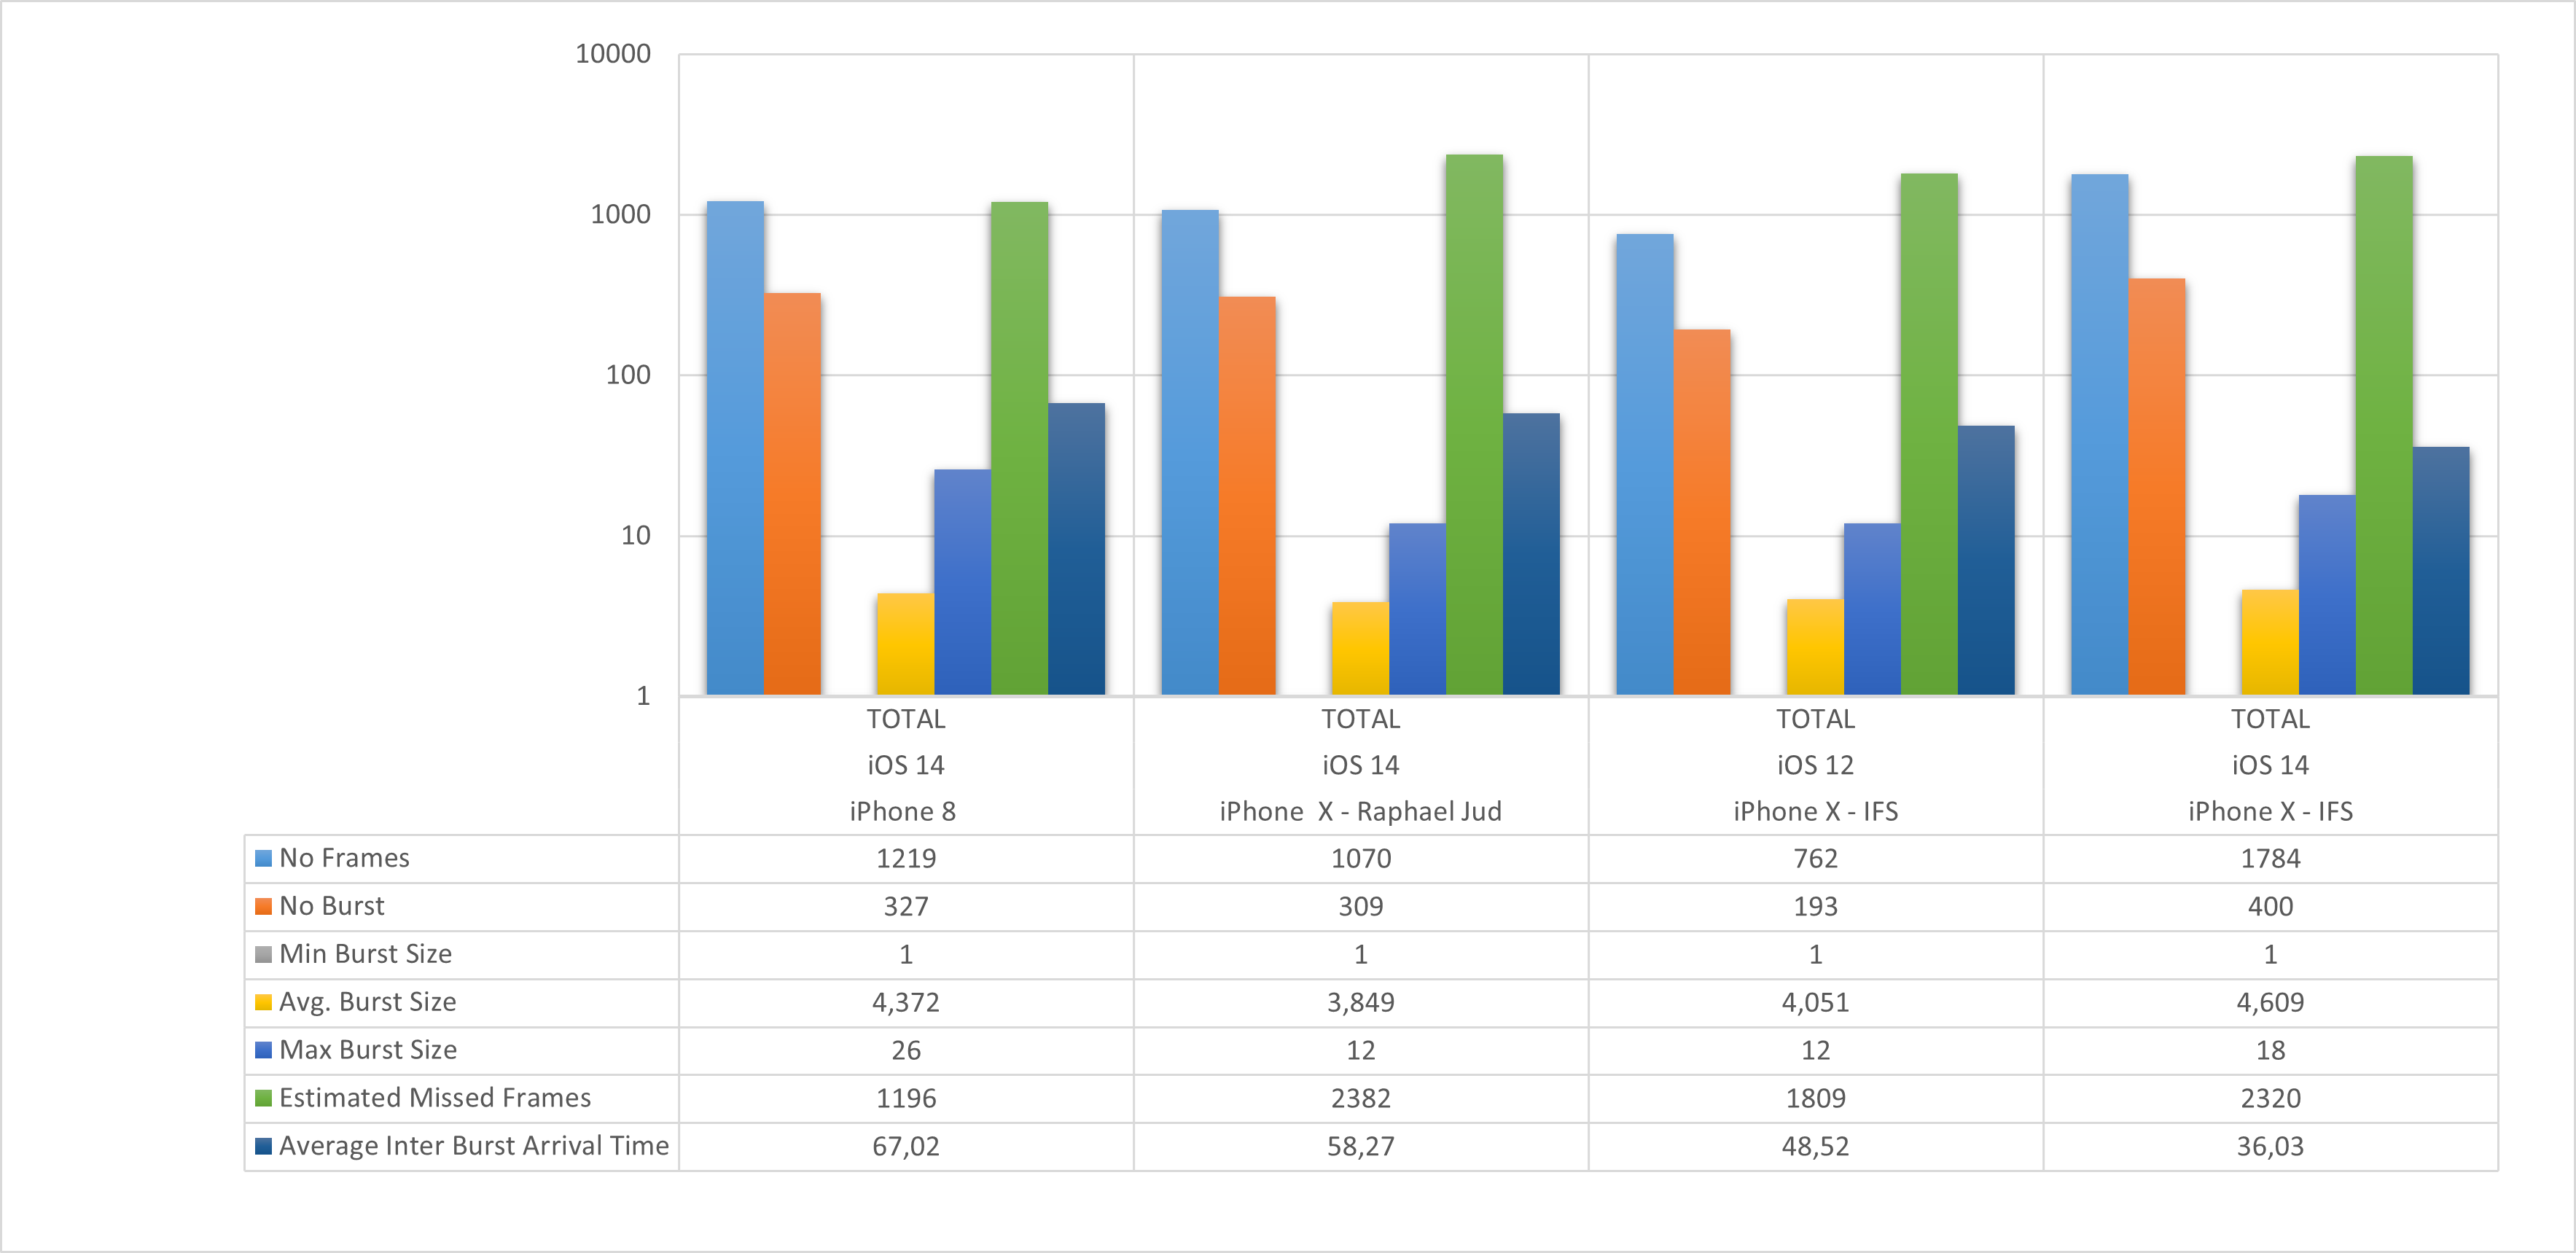
\includegraphics[width=1\linewidth]{Experiments/IOS-Total.png}
        \caption{Gesamtergebnis der iOS-Messungen}
        \label{figure:totaliosmeasurements}
    \end{figure}
\end{landscape}

\begin{figure}[h!]
    \centering
    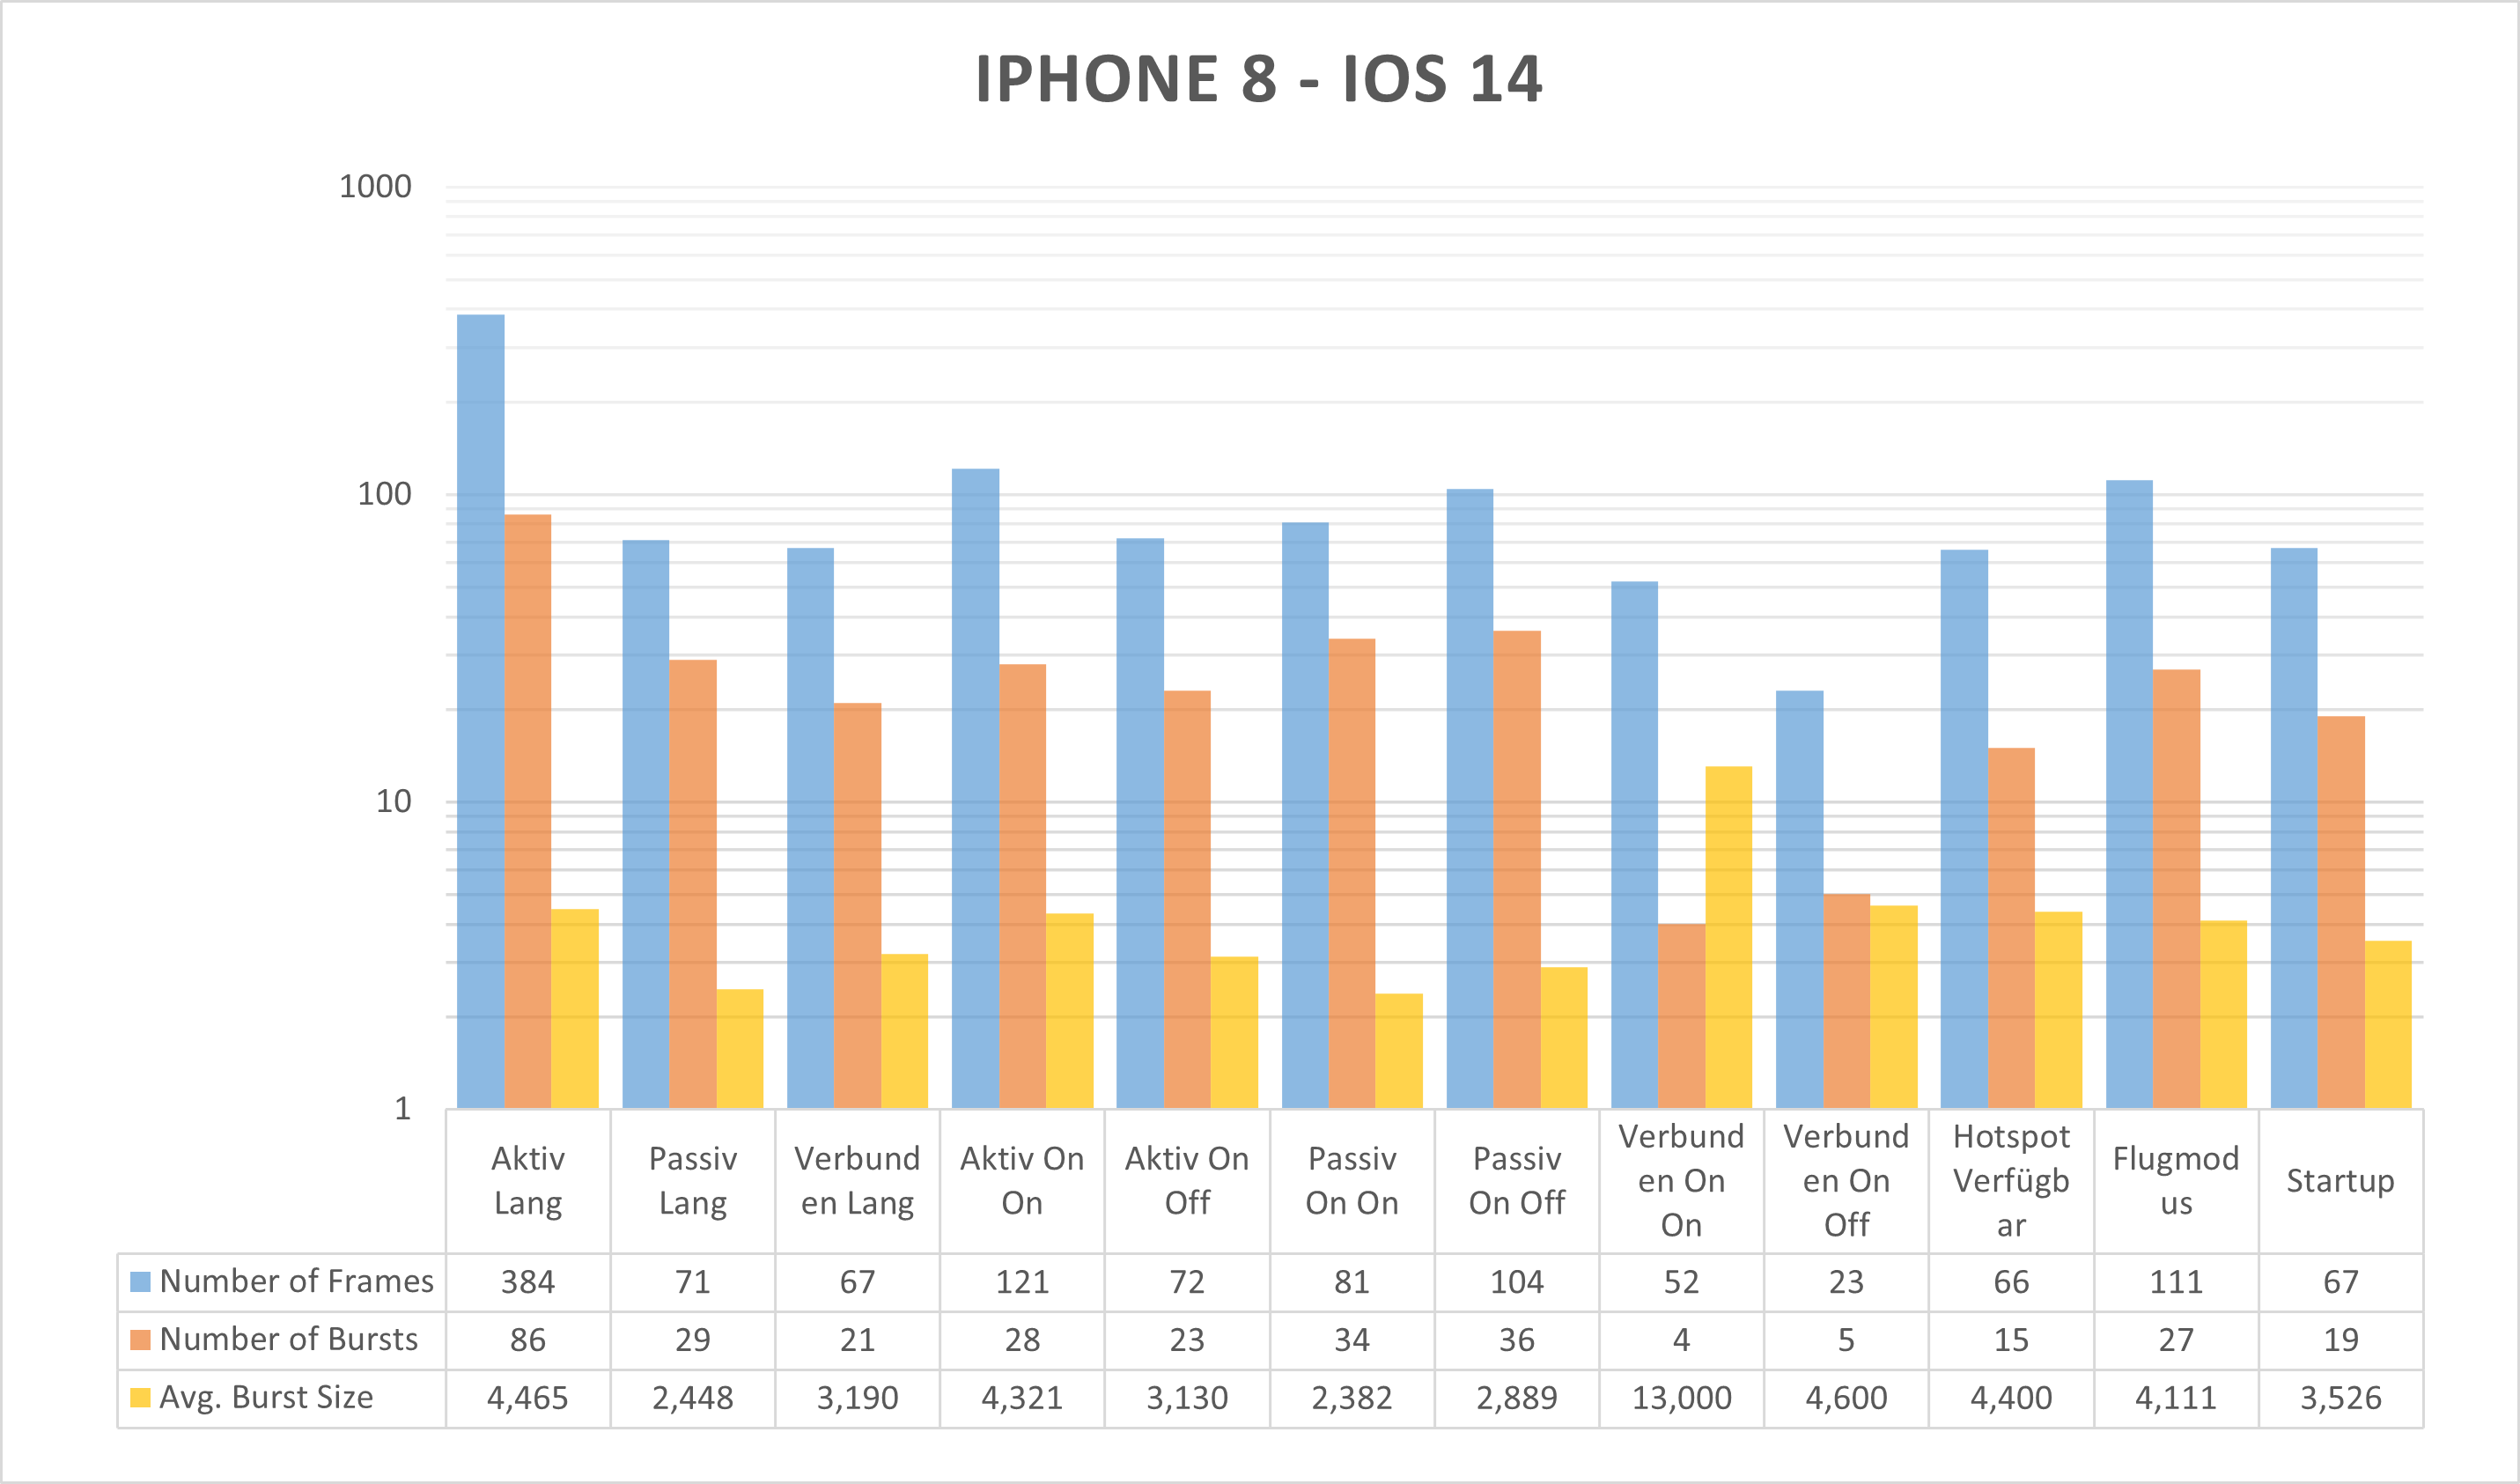
\includegraphics[width=1\linewidth]{Experiments/IPhone8-14.png}
    \caption{Messergebnisse iPhone 8 - iOS 14.0.1}
    \label{figure:iosmeasurementsbycategoryiphone-8-14}
\end{figure}

\begin{figure}[h!]
    \centering
    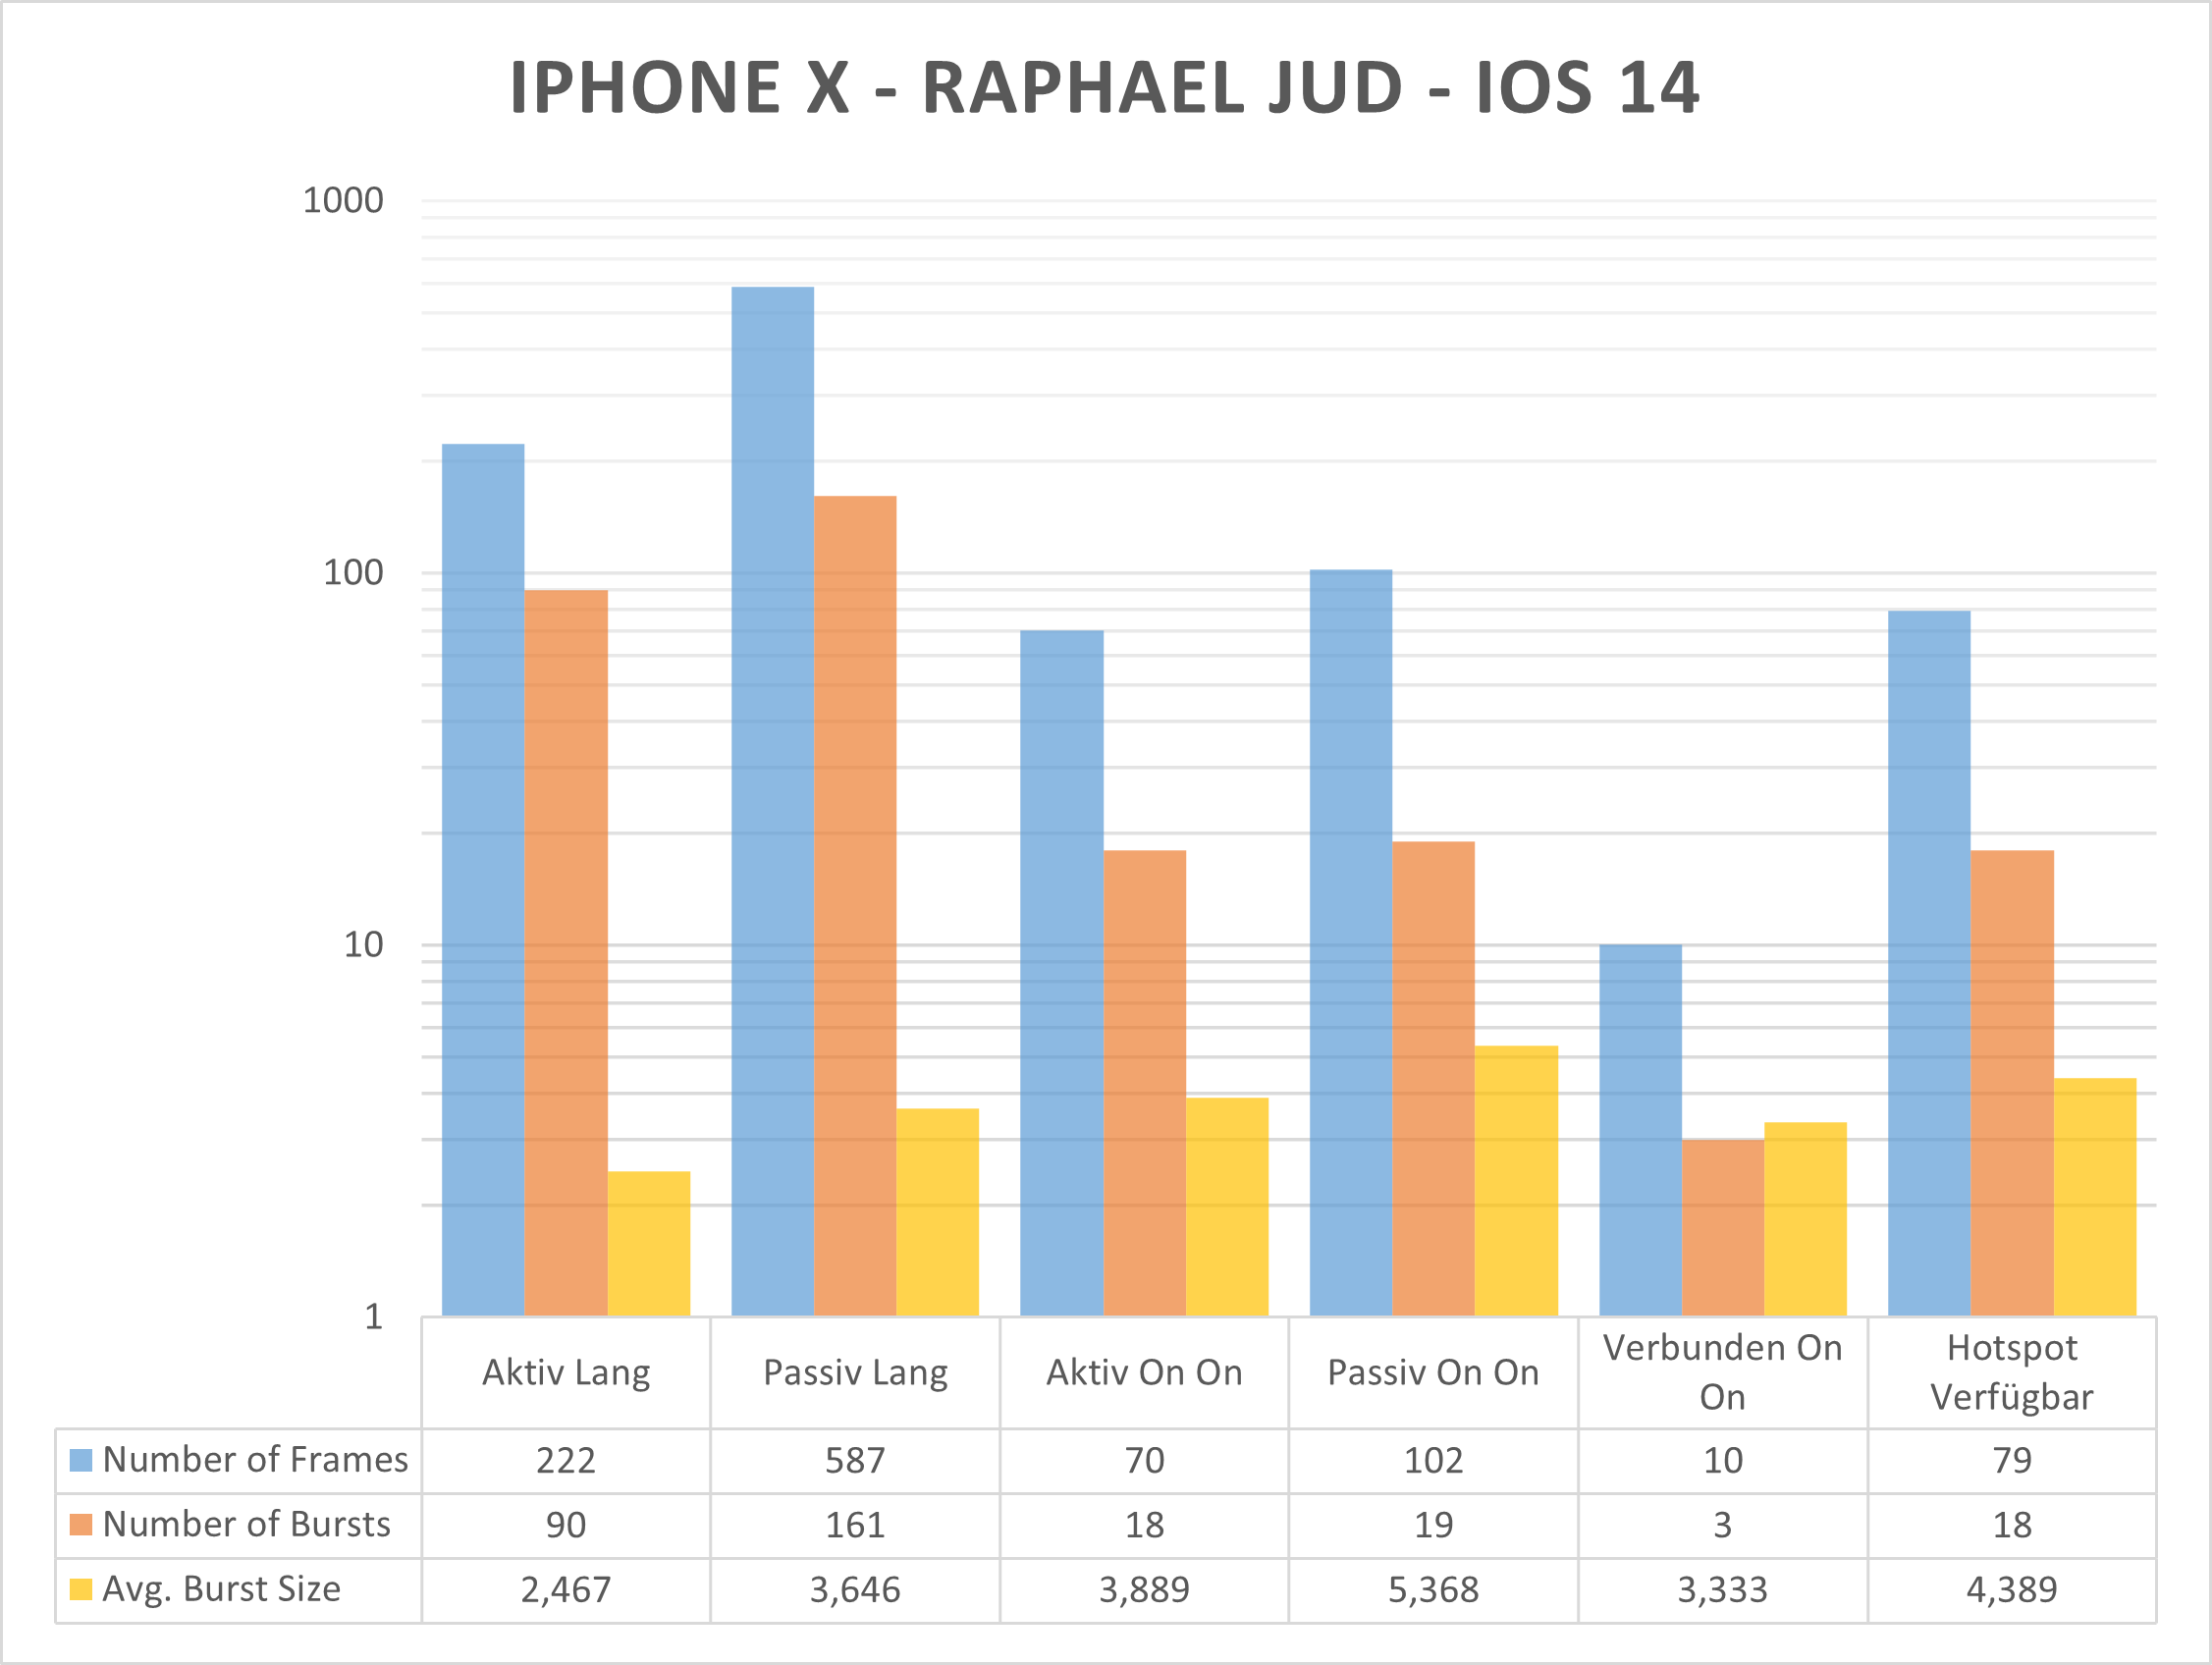
\includegraphics[width=1\linewidth]{Experiments/IPhoneX-RaphaelJud-14.png}
    \caption{Messergebnisse iPhone X - Raphael Jud - iOS 14.0.1}
    \label{figure:iosmeasurementsbycategoryiphone-se-14}
\end{figure}

\begin{figure}[h!]
    \centering
    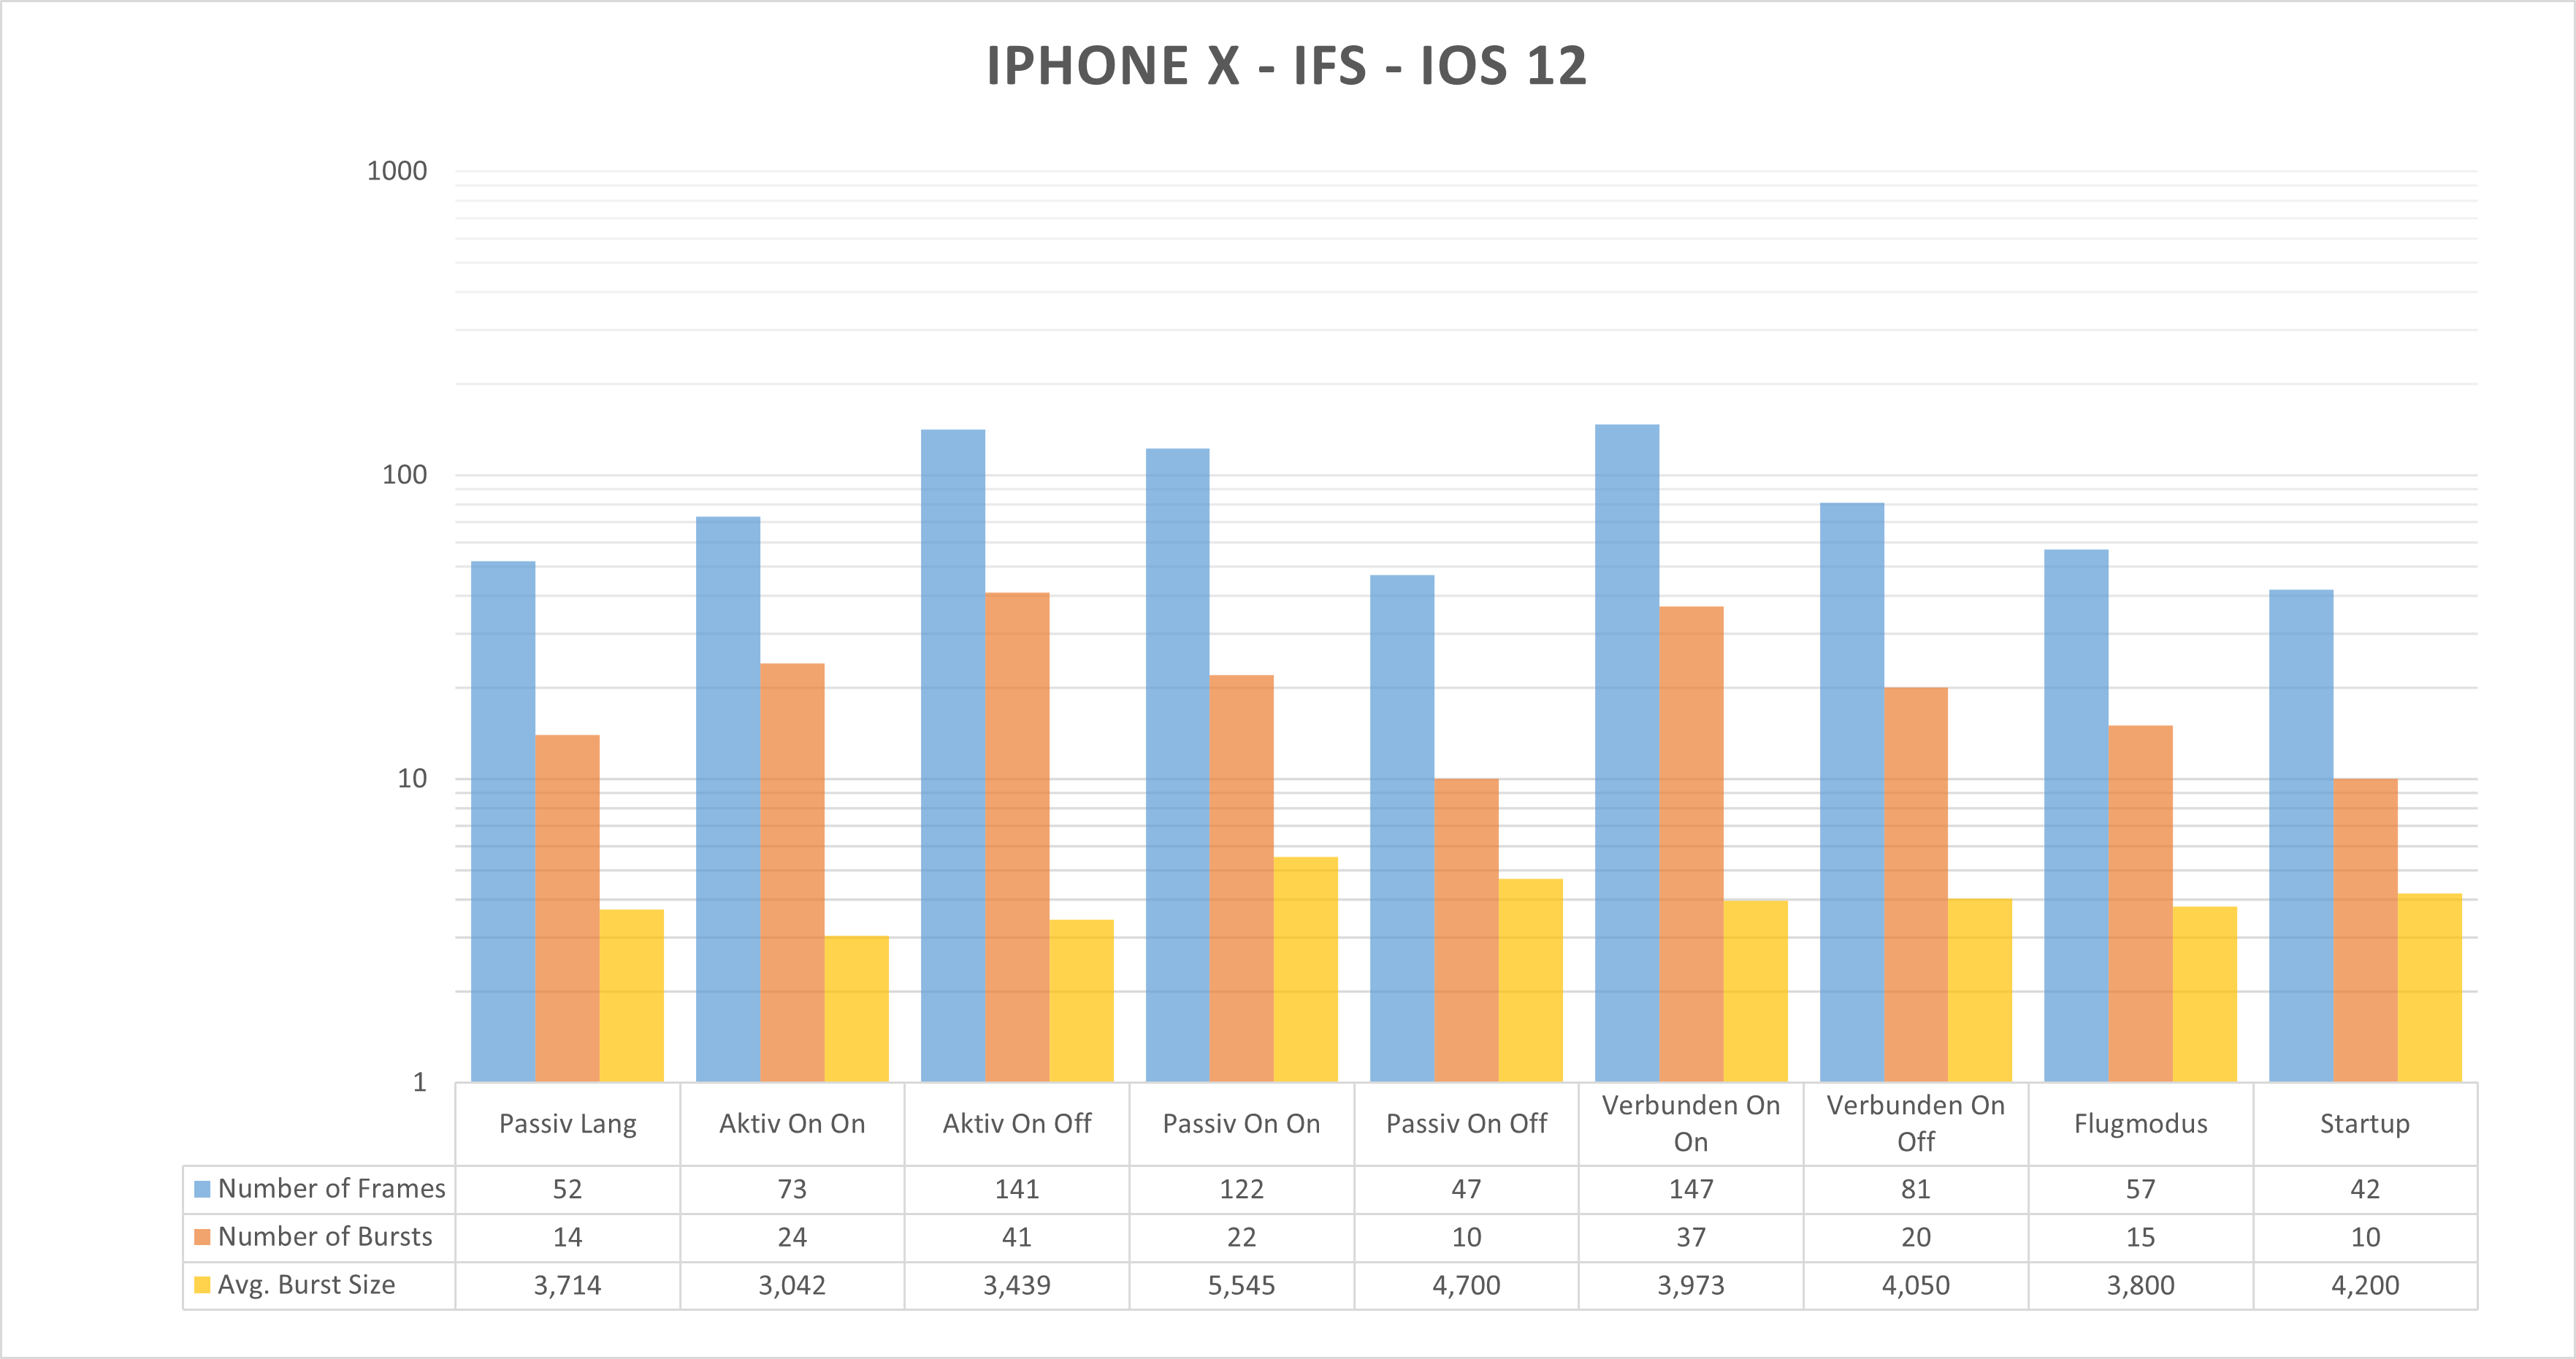
\includegraphics[width=1\linewidth]{Experiments/IPhoneX-IFS-12.png}
    \caption{Messergebnisse iPhone X - IFS - iOS 12.3.1}
    \label{figure:iosmeasurementsbycategoryiphone-x-12}
\end{figure}

\begin{figure}[h!]
    \centering
    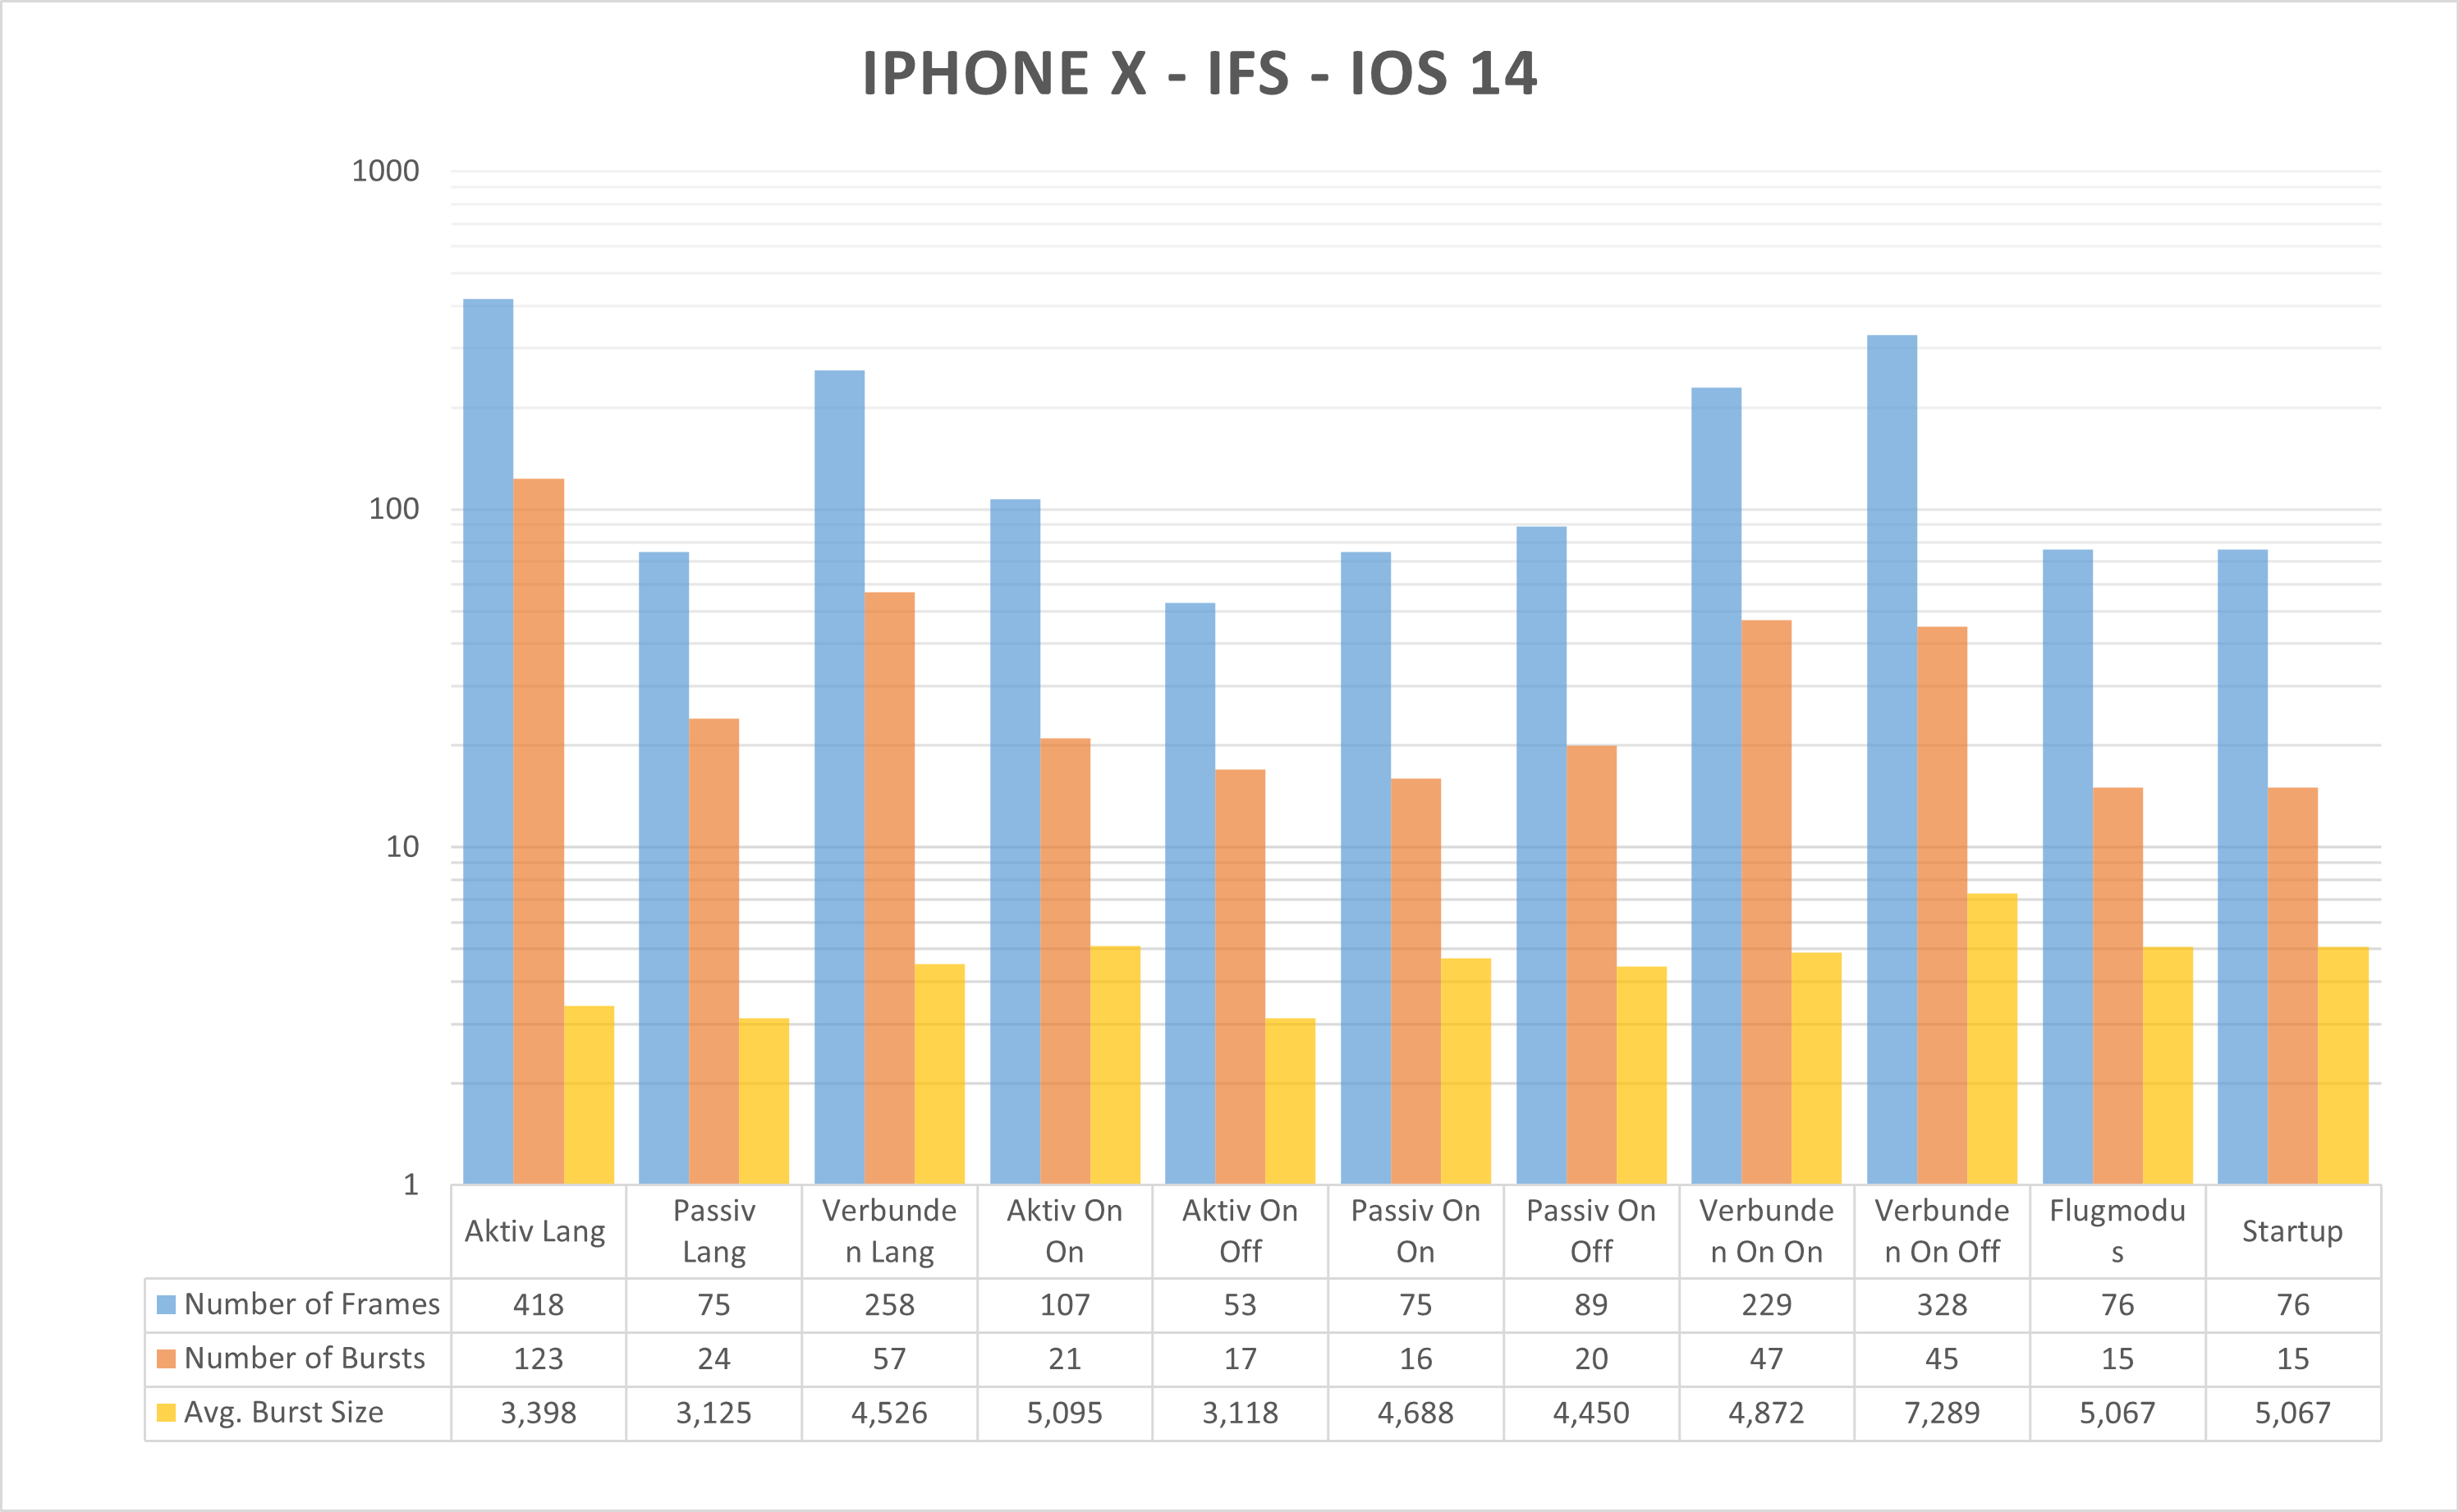
\includegraphics[width=1\linewidth]{Experiments/IPhoneX-IFS-14.png}
    \caption{Messergebnisse iPhone X - IFS - iOS 14.0.1}
    \label{figure:iosmeasurementsbycategoryiphone-x-14}
\end{figure}

\clearpage

\subsubsection*{Erkenntnisse aus den iOS-Messungen}
In total $4835$ aufgezeichneten Probe-Requests sind im Schnitt jeweils $4.22$ 
Frames pro Burst mit einer durchschnittlichen Zwischenankunftszeit von $52.46 s$
gemessen worden. Die Bursts haben eine Grösse zwischen einem und 26 Frames.

Anhand der Sequenznummern innerhalb eines Bursts kann abgeschätzt werden, wie 
viele Frames im Burst nicht aufgezeichnet (verpasst) werden.
In den iOS-Messungen wurden schätzungsweise $7707$ Frames verpasst.
Eine mögliche Erklärung für die hohe Anzahl verpasster Frames ist, dass
iPhones zwischen einzelnen Frames den Kanal wechseln bzw. Probe-Requests auf 
wechselnden Kanälen aussenden, anstatt die Probes für einen Kanal zu gruppieren.

Bei genauerer Betrachtung der pcap oder JSON-Dateien zu den einzelnen Messungen
fällt auf, dass iPhones IE-Felder gemäss den Tabellen~\ref{table:ioscommoniefields}, 
\ref{table:iosuncommoniefields} und~\ref{table:iosvendorspecificiefields} 
beinhalten.

\begin{table}[h!]
    \centering
    \begin{tabular}{|c|c|c|c|c|}
        \hline
        \textbf{Tag-NR} & \textbf{0} & \textbf{1} & \textbf{50} & \textbf{3} \\
        \textbf{Tag-Name} & \textbf{SSID} & \textbf{Supported Rates} & \textbf{Ex. Supp. Rates} & \textbf{DS Params Set} \\
        \hline 
        Geräte & alle & alle & alle & alle \\
        \hline
    \end{tabular}
    \caption{IE-Felder, die in allen Messungen vorkommen
    \label{table:ioscommoniefields}}  
\end{table}

\begin{table}[h!]
    \centering
    \begin{tabular}{|c|c|c|c|}
        \hline
        \textbf{Tag-NR} & \textbf{45} & \textbf{127} & \textbf{107} \\
        \textbf{Tag-Name} & \textbf{HT Capabilities} & \textbf{Extended Capabilities} & \textbf{Interworking} \\
        \hline 
        Phones  & alle & alle & alle \\
        \hline
    \end{tabular}
    \caption{IE-Felder der einzelnen iPhones
    \label{table:iosuncommoniefields}}  
\end{table}

Es wird davon ausgegangen, dass die IE-Felder mit den Nummern 0, 1, 50, 3, 45 
und 127 in allen iOS-Geräten verwendet werden. 
Der Interworking Tab mit der Tagnummer 107 wird in verschiedenen Messungen 
mitgesendet, es kann aber aus den Ergebnissen keine Regelmässigkeit herausgelesen
werden, nach welchen Voraussetzungen der Tag verwendet wird.

\clearpage 

\begin{table}[h!]
    \centering
    \begin{tabular}{|c|c|c|c|}
        \hline
        &  \textbf{Apple}  & \textbf{Microsoft Corp.} & \textbf{Broadcom} \\
        \hline 
        iPhone 8 & x  &  & \\
        iPhone X - Raphael Jud - 14 & & & \\
        iPhone X - IFS - 12 & x  & x & x \\
        iPhone X - IFS - 14 &  & x & \\
        \hline
    \end{tabular}
    \caption{Herstellerspezifische Felder (Vendor Specific - 221)
    \label{table:iosvendorspecificiefields}}  
\end{table}

Pro Burst wird sowohl die MAC-Adresse als auch die Sequenznummer zufallsgeneriert.
In ca $53\%$ aller gemessenen iOS-MAC-Adressen ist das lokale Bit gesetzt, was bei 
zufallsgenerierten Adressen dem erwarteten Wert von $50\%$ nahekommt.
Alle iPhones verwenden, wenn sie mit einem Access-Point verbunden sind, ihre 
Korrekte MAC-Adresse. Weiterhin haben das iPhone 8 sowie das iPhone X mit der 
iOS-Version 12 in sämtlichen MAC-Adressen das lokale Bit gesetzt.

\subsubsection*{Vergleich mit den MAC-Adressen der Vorarbeit}
In der Vorarbeit wurde eine Tabelle mit den häufigsten auftretenden OUI's von
MAC-Adressen erstellt. Die in dieser Arbeit gemessenen Adressen wurde mit der
Tabelle der Vorarbeit verglichen, um allenfalls Muster zu erkennen. 
Die OUIs der Vorarbeit sind in der Tabelle~\ref{table:commonouis} abgebildet.
CSV-Listen mit den MAC-Adressen aus den Messungen sind im Repository im 
Ordner "Experimente" zu finden.

\begin{table}[h!]
    \centering
    \begin{tabular}{|c|c|c|}
        \hline
        00:B5:D0 & 04:79:70 & 04:F0:21 \\
        \hline
        04:FE:A1 & 60:F1:89 & 7C:0B:C6 \\
        \hline 
        80:00:0B & 84:98:66 & 9C:E0:63 \\
        \hline 
        B8:27:EB & E0:9D:31 & EC:9B:F3 \\
        \hline
        F0:42:1C & & \\
        \hline 
    \end{tabular}
    \caption{Häufigste OUIs in der Vorarbeit
    \label{table:commonouis}}  
\end{table}

Es wurden keine Übereinstimmungen der MAC-Adressen aus den Messungen mit den 
OUIs der Vorarbeit gefunden.
\clearpage
\section{Android-Messungen
\label{section:androidmeasurements}}
Nachfolgend sind die Messungen auf Mobilgeräten mit Android-Betriebs-systemen 
und daraus gewonnene Erkenntnisse beschrieben.

Gesamthaft wurden 70 Einzelmessungen in 28 Stunden und 40 Minuten durchgeführt.

\subsection{Versuchsdurchführung}
Die im Unterabschnitt~\ref{subsection:plannedexperiments} genannten
Messungen wurden auf insgesamt neun Android-Geräten durchgeführt, welche in der 
Tabelle~\ref{table:measuredandroiddevices} aufgeführt werden.

\begin{table}[h!]
	\centering
	\begin{tabular}{|c|c|c|}
		\hline
        \textbf{Gerätetyp} & \textbf{Android-Version} & \textbf{Besitzer} \\
        \hline
        Samsung A51 & Android 10 & Janik Schlatter \\
        Fairphone 3+ & Android 10 & Mike Schmid \\
        Samsung Galaxy S8 & Android 9 & IFS \\
        Samsung Galaxy S8 & Android 9 & IFS \\
        Samsung Galaxy S8 & Android 9 & Janik Schlatter \\
        Samsung Galaxy S8 & Android 9 & Jenny Bösch \\
        Samsung Galaxy S9 & Android 10 & IFS \\
        Samsung Galaxy S20+ &  Android 10 & IFS \\
        Google Pixel 3  & Android 11 & IFS \\
        \hline
    \end{tabular}
    \caption{Gemessene Android-Geräte
    \label{table:measuredandroiddevices}}  
\end{table}

Die Messungen auf allen Geräten ausser den vier Galaxy S8 Geräten wurden komplett
durchgeführt. Die S8 mit Android 9 verschleiern ihre MAC-Adresse in Probe-Requests
nicht, weswegen auf diesen vier Geräten nur 20-minütige Aktivtests durchgeführt
wurden. 

Weiterhin stand für die zweite Woche in den Android-Messungen der Wave-Xpert, 
ein WLAN-Messgerät mit dem mehrere Kanäle gleichzeitig gemessen werden können,
zur Verfügung. Mit dem WaveXpert wurden die Messungen mit dem Fairphone 3+ und 
Messungen mit mehreren parallel laufenden Geräten durchgeführt.
Diese parallelen Messungen dienen der Verifikation eines Prototypen mit Daten, 
die ein realistischeres Umfeld darstellen, deren Parameter (Anzahl Geräte, 
Laufzeit, welche Geräte verbunden sind, etc.) aber beeinflusst werden können.

\subsection{Ergebnisse}
Die folgenden Messergebnisse konnten in den Messungen produziert werden.

\subsubsection*{Probe-Requests}
In der Tabelle~\ref{table:androidproberesults} ist ersichtlich, wie viele Probe 
Requests pro Messung aufgezeichnet wurden, wie viele davon in Bursts gruppiert
waren, die minimale, durchschnittliche und maximale Burstgrösse sowie eine 
Schätzung der nicht aufgezeichneten Frames und die durchschnittliche 
Zwischenankunftszeit zwischen zwei Bursts.

\begin{landscape}
    \begin{table}[h!]
        \small
	    \centering
        \begin{tabular}{|c|c|c|c|c|c|c|c|c|}
            \hline
            \textbf{Gerät} & \textbf{Android}  & \textbf{Anzahl} & \textbf{Anzahl} & \textbf{min.} & \textbf{avg.} & \textbf{max.} & \textbf{Verpasste} & \textbf{Zwischen-}\\
             & \textbf{Version} & \textbf{Probe-Requests} & \textbf{Bursts} & \textbf{Burstgrösse} & \textbf{Burstgrösse} & \textbf{Burstgrösse} & \textbf{Frames} & \textbf{ankunftszeit}\\
            \hline
            \shortstack{Samsung \\ A51 } &  10 & \phantom{0}412 & \phantom{00}61 & 2 & \phantom{0}6,409 & 12 & \phantom{0}270 & 276,04 s \\
            \hline
            \shortstack{Samsung \\ Galaxy S9 } &  10 & \phantom{0}384 & \phantom{0}125 & 1 & \phantom{0}2,897 & \phantom{0}7 & \phantom{0}632 & 211,88 s \\
            \hline
            \shortstack{Samsung \\ Galaxy S20+ } &  10 & \phantom{0}489 & \phantom{0}303 & 1 & \phantom{0}1,889 & \phantom{0}2 & \phantom{0}161 & 118,00 s \\
            \hline
            \shortstack{Google \\ Pixel 3 } &  11 & 5048 & \phantom{0}960 & 1 & \phantom{0}4,415 & 15 & 2076 & 32,99 s \\
            \hline
            \shortstack{Samsung \\ Galaxy S8 } & \phantom{0}9 & \phantom{00}44 &\phantom{00} 12 & 2 & \phantom{0}3,667 & \phantom{0}6 & \phantom{00}32 & \phantom{0}94,27 s \\
            \hline
            \shortstack{Samsung \\ Galaxy S8 } &  \phantom{0}9 & \phantom{00}60 & \phantom{00}11 & 2 & \phantom{0}5,455 & 10 & \phantom{00}64 & 101,21 s \\
            \hline
            \shortstack{Samsung \\ Galaxy S8 } &  \phantom{0}9 & \phantom{0}149 & \phantom{00}20 & 1 & \phantom{0}7,450 & 13 & \phantom{0}149 & \phantom{0}55,78 s \\
            \hline
            \shortstack{Samsung \\ Galaxy S8 } &  \phantom{0}9 & \phantom{0}101 & \phantom{00}14 & 4 & \phantom{0}7,214 & 11 & \phantom{0}200 & \phantom{0}80,29 s \\
            \hline
            Fairphone 3+ &  10 & 2329 & \phantom{0}386 & 1 & 10,283 & 25 & \phantom{0}744 & \phantom{0}93,69 s \\
            \hline
            TOTAL & & 9016 & 1892 & 1 & \phantom{0}5,520 & 25 & 4328 & 118,24 s \\
            \hline
        \end{tabular}
        \caption{Ergebnisse der Android-Messungen
        \label{table:androidproberesults}}  
    \end{table}
    Die genauen Auswertungen der Messergebnisse finden sich im 
    Anhang~\ref{chapter:appendix:experimentaldata}. 
    Die Daten sind auf dem Repository im Ordner "Experimente" in den jeweiligen Unterordnern
    zu finden.

    \clearpage

    Nachfolgend sind in den Abbildungen die Graphische Auswertung nach Gesamtzahl
    (Abbildung~\ref{figure:totalandroidmeasurements}) der Messwerte und die Messergebnisse nach Kategorie für
    die einzelnen Android-Geräte (Abbildungen~\ref{figure:androidmeasurementsbycategorys8}
    bis~\ref{figure:androidmeasurementsbycategorypixel}) dargestellt.

    \begin{figure}[h!]
        \centering
        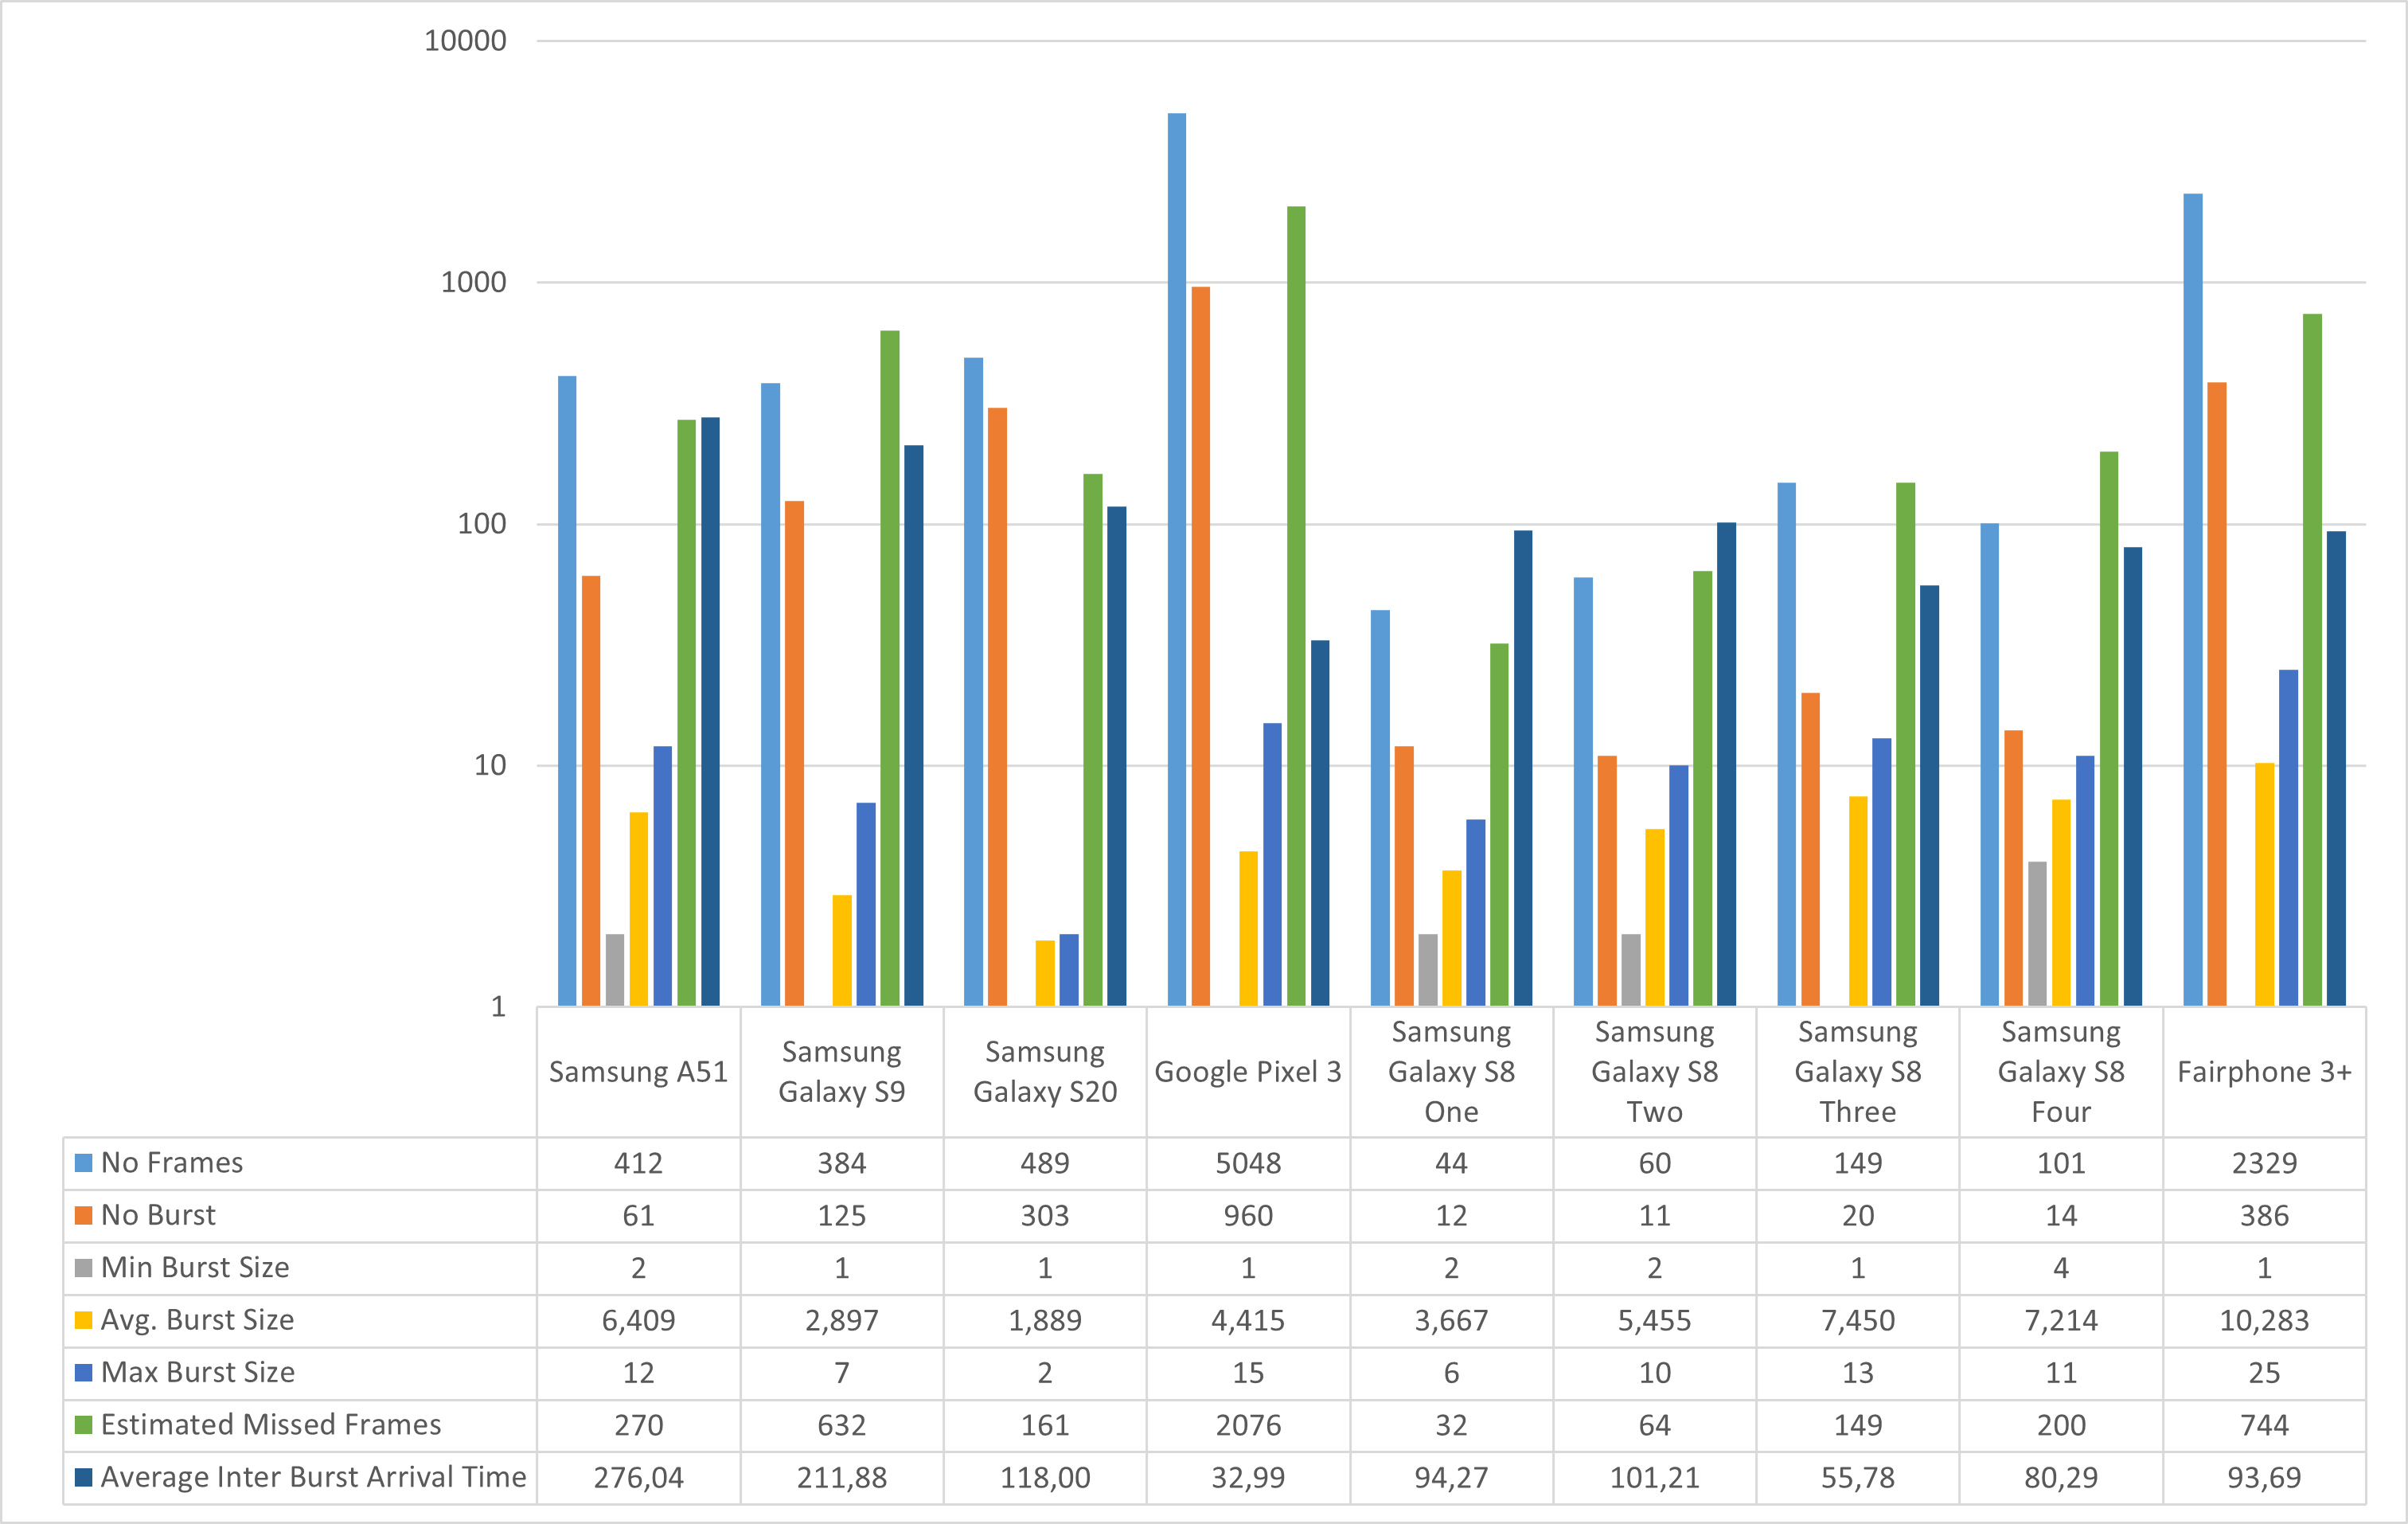
\includegraphics[width=0.75\linewidth]{Experiments/Android-Total.png}
        \caption{Gesamtergebnis der Android-Messungen}
        \label{figure:totalandroidmeasurements}
    \end{figure}
\end{landscape}

\clearpage

\begin{figure}[h!]
    \centering
    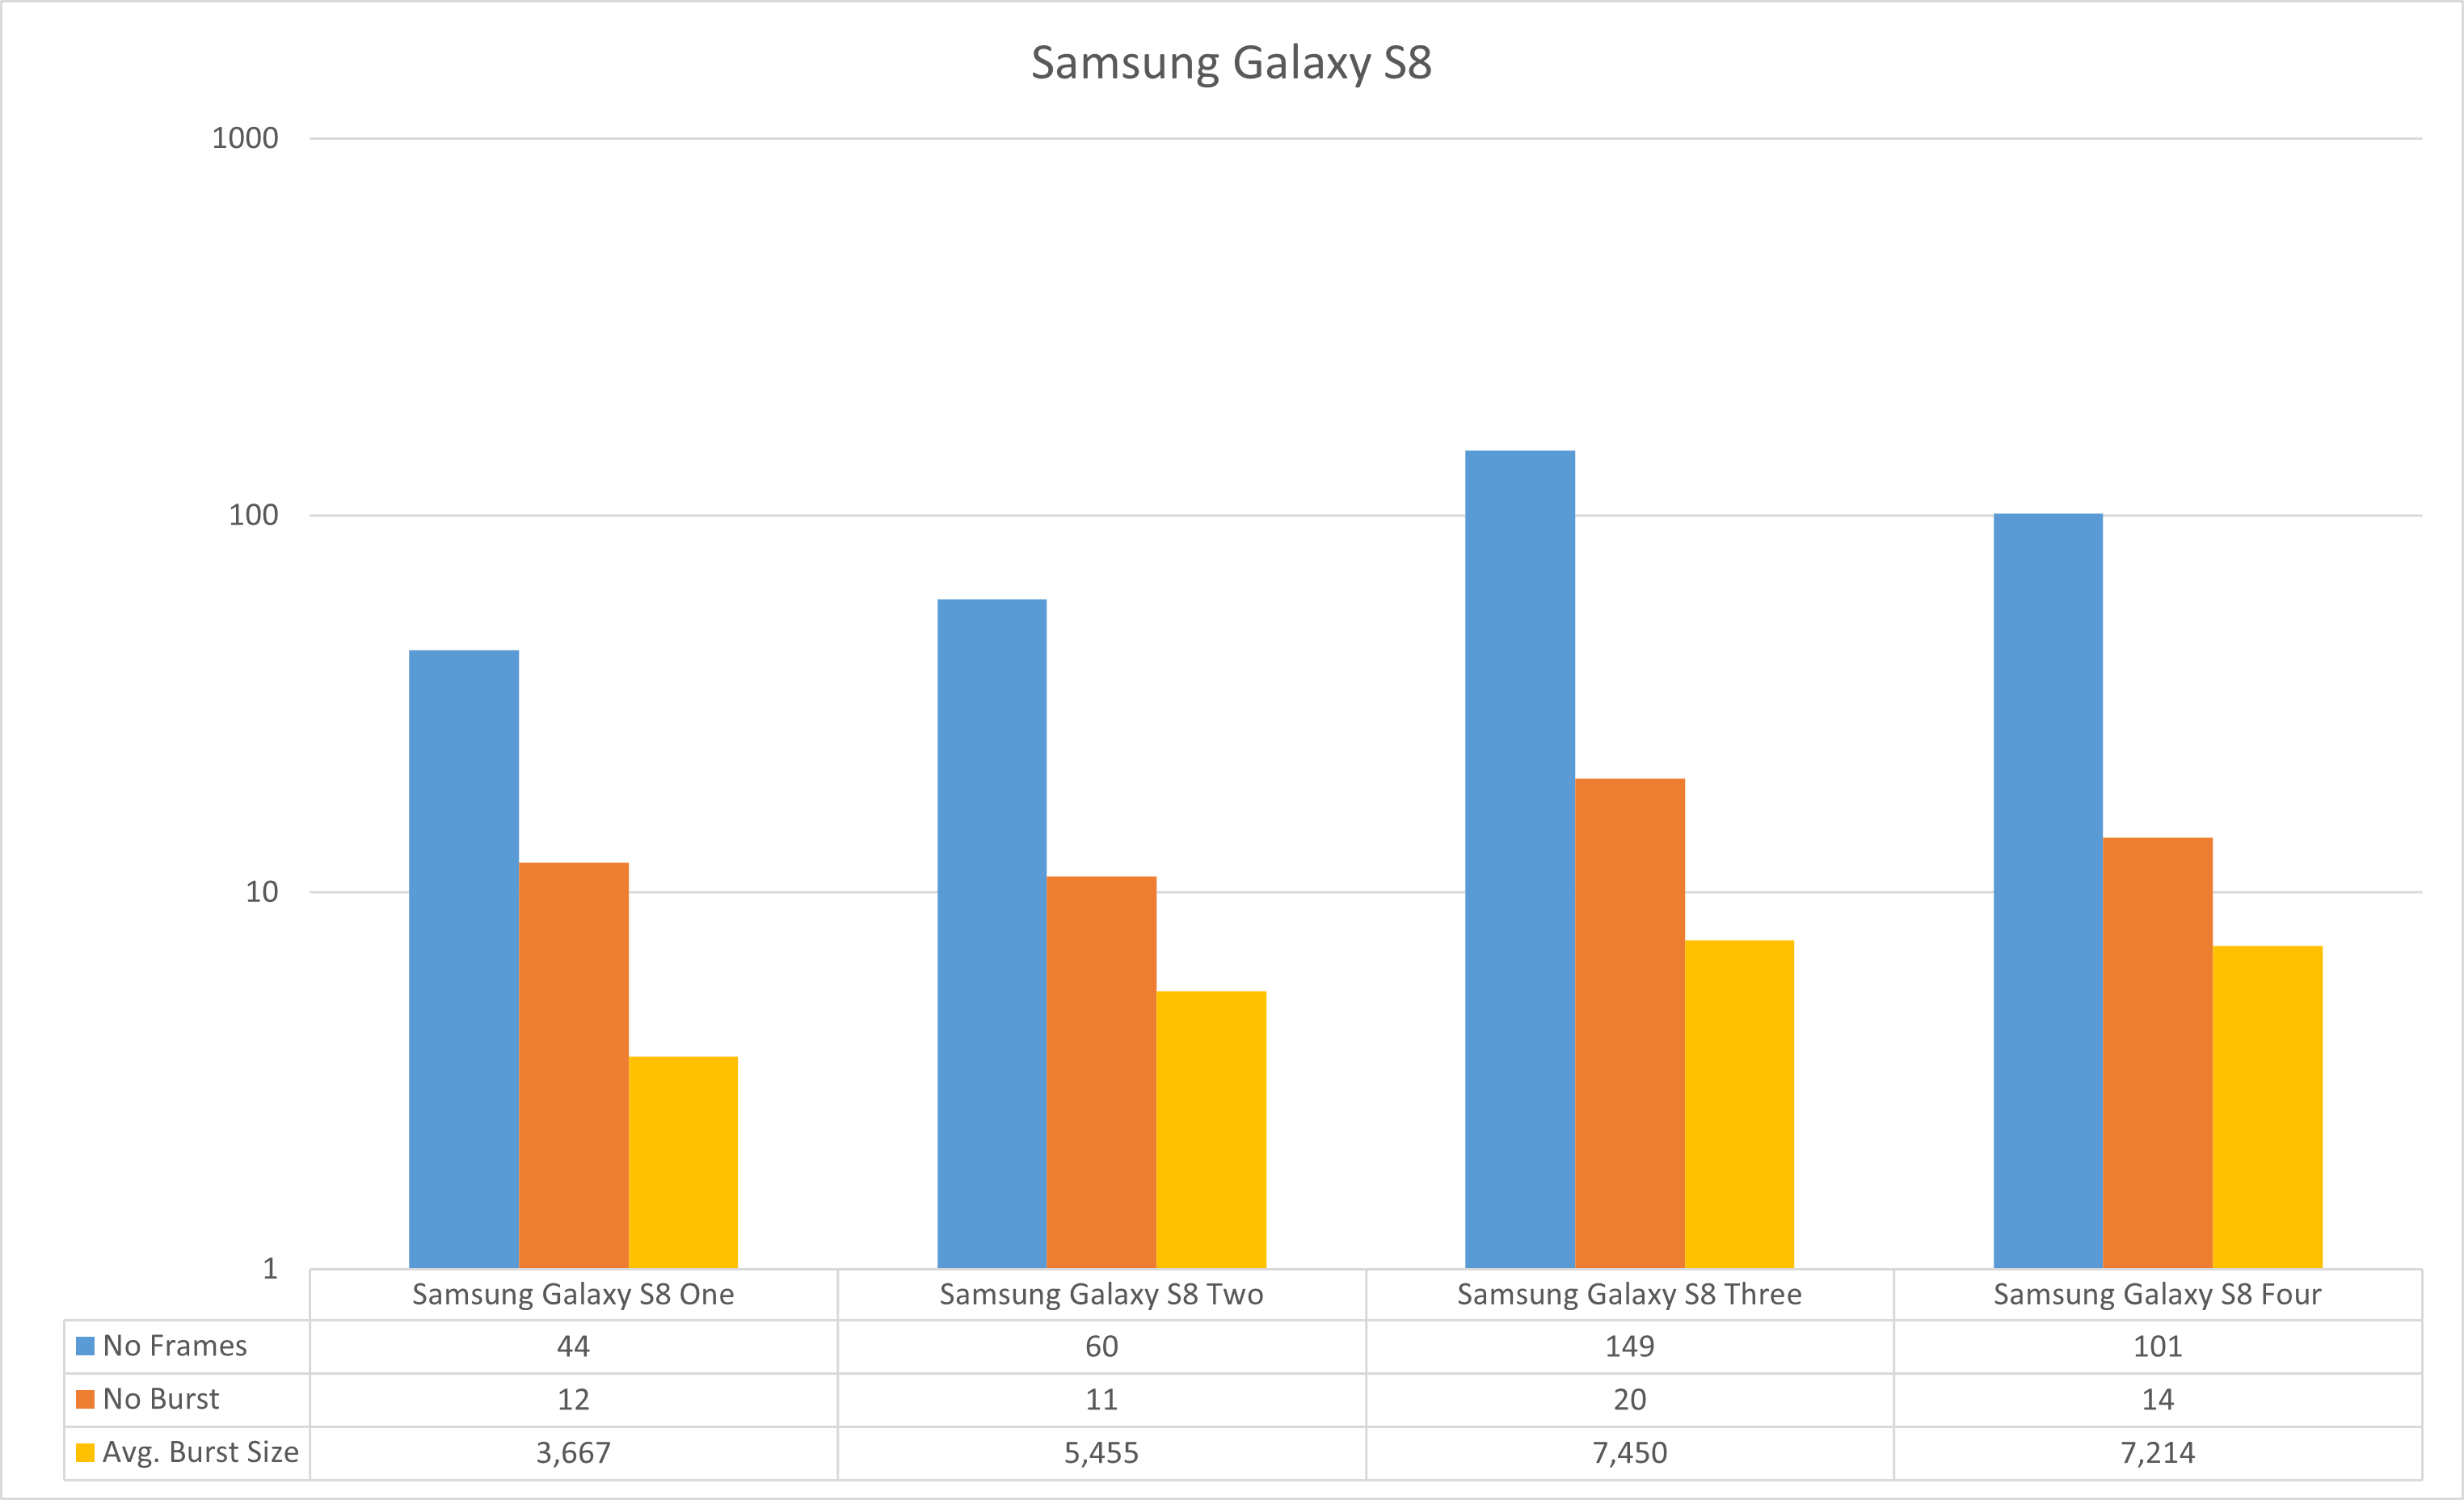
\includegraphics[width=1\linewidth]{Experiments/S8-Gruppe.png}
    \caption{Messergebnisse der vier Samsung Galaxy S8-Geräte mit Android 9}
    \label{figure:androidmeasurementsbycategorys8}
\end{figure}

In den Messungen der Samsung Galaxy S8 ist aufgefallen, dass diese bei 
Probe-Requests ihre echte Gerätemacadresse verwenden. Dieses Verhalten ist bei 
allen vier Geräten ersichtlich und lässt darauf schliessen, dass alle Samsung 
Galaxy Geräte der S8-Generation mit Android die MAC-Adresse nicht verschleiern.
(Sofern nicht über den Developermodus die seit Android 6 verfügbare Option 
gesetzt wurde, die MAC-Adressen zu randomisieren)

\clearpage

\begin{figure}[h!]
    \centering
    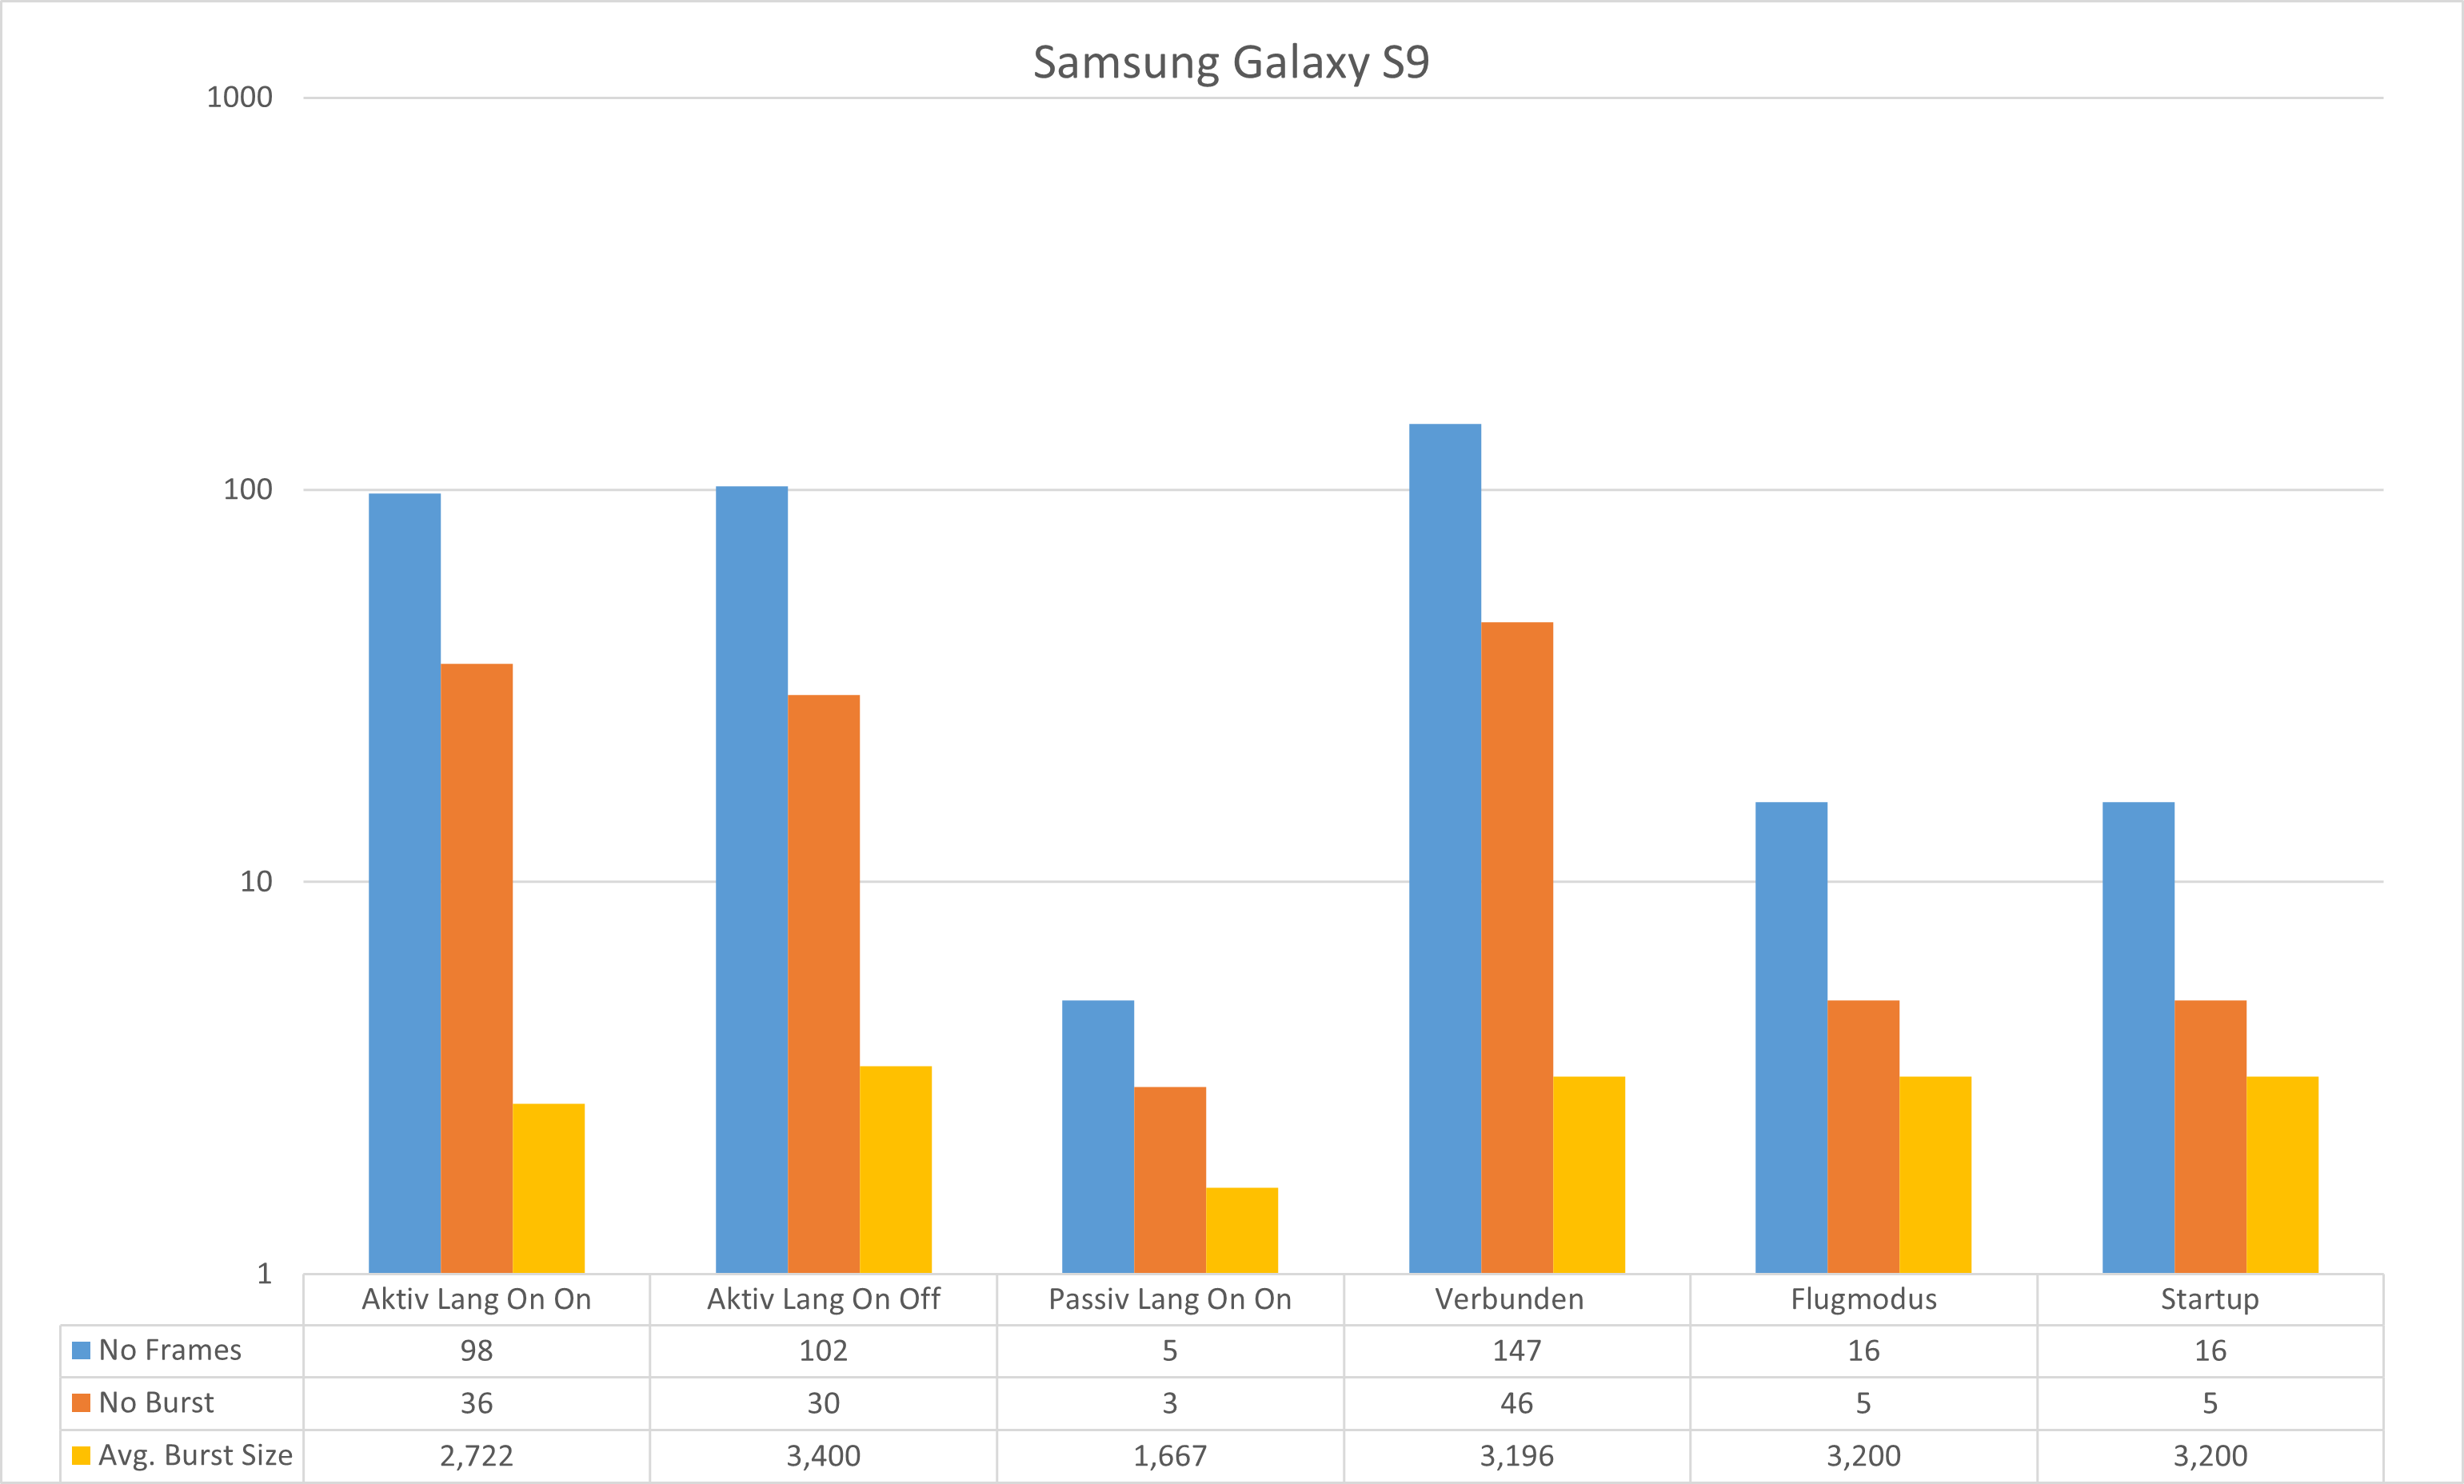
\includegraphics[width=1\linewidth]{Experiments/S9-10.png}
    \caption{Messergebnisse Samsung Galaxy S9 - Android 10}
    \label{figure:androidmeasurementsbycategorys9}
\end{figure}

\begin{figure}[h!]
    \centering
    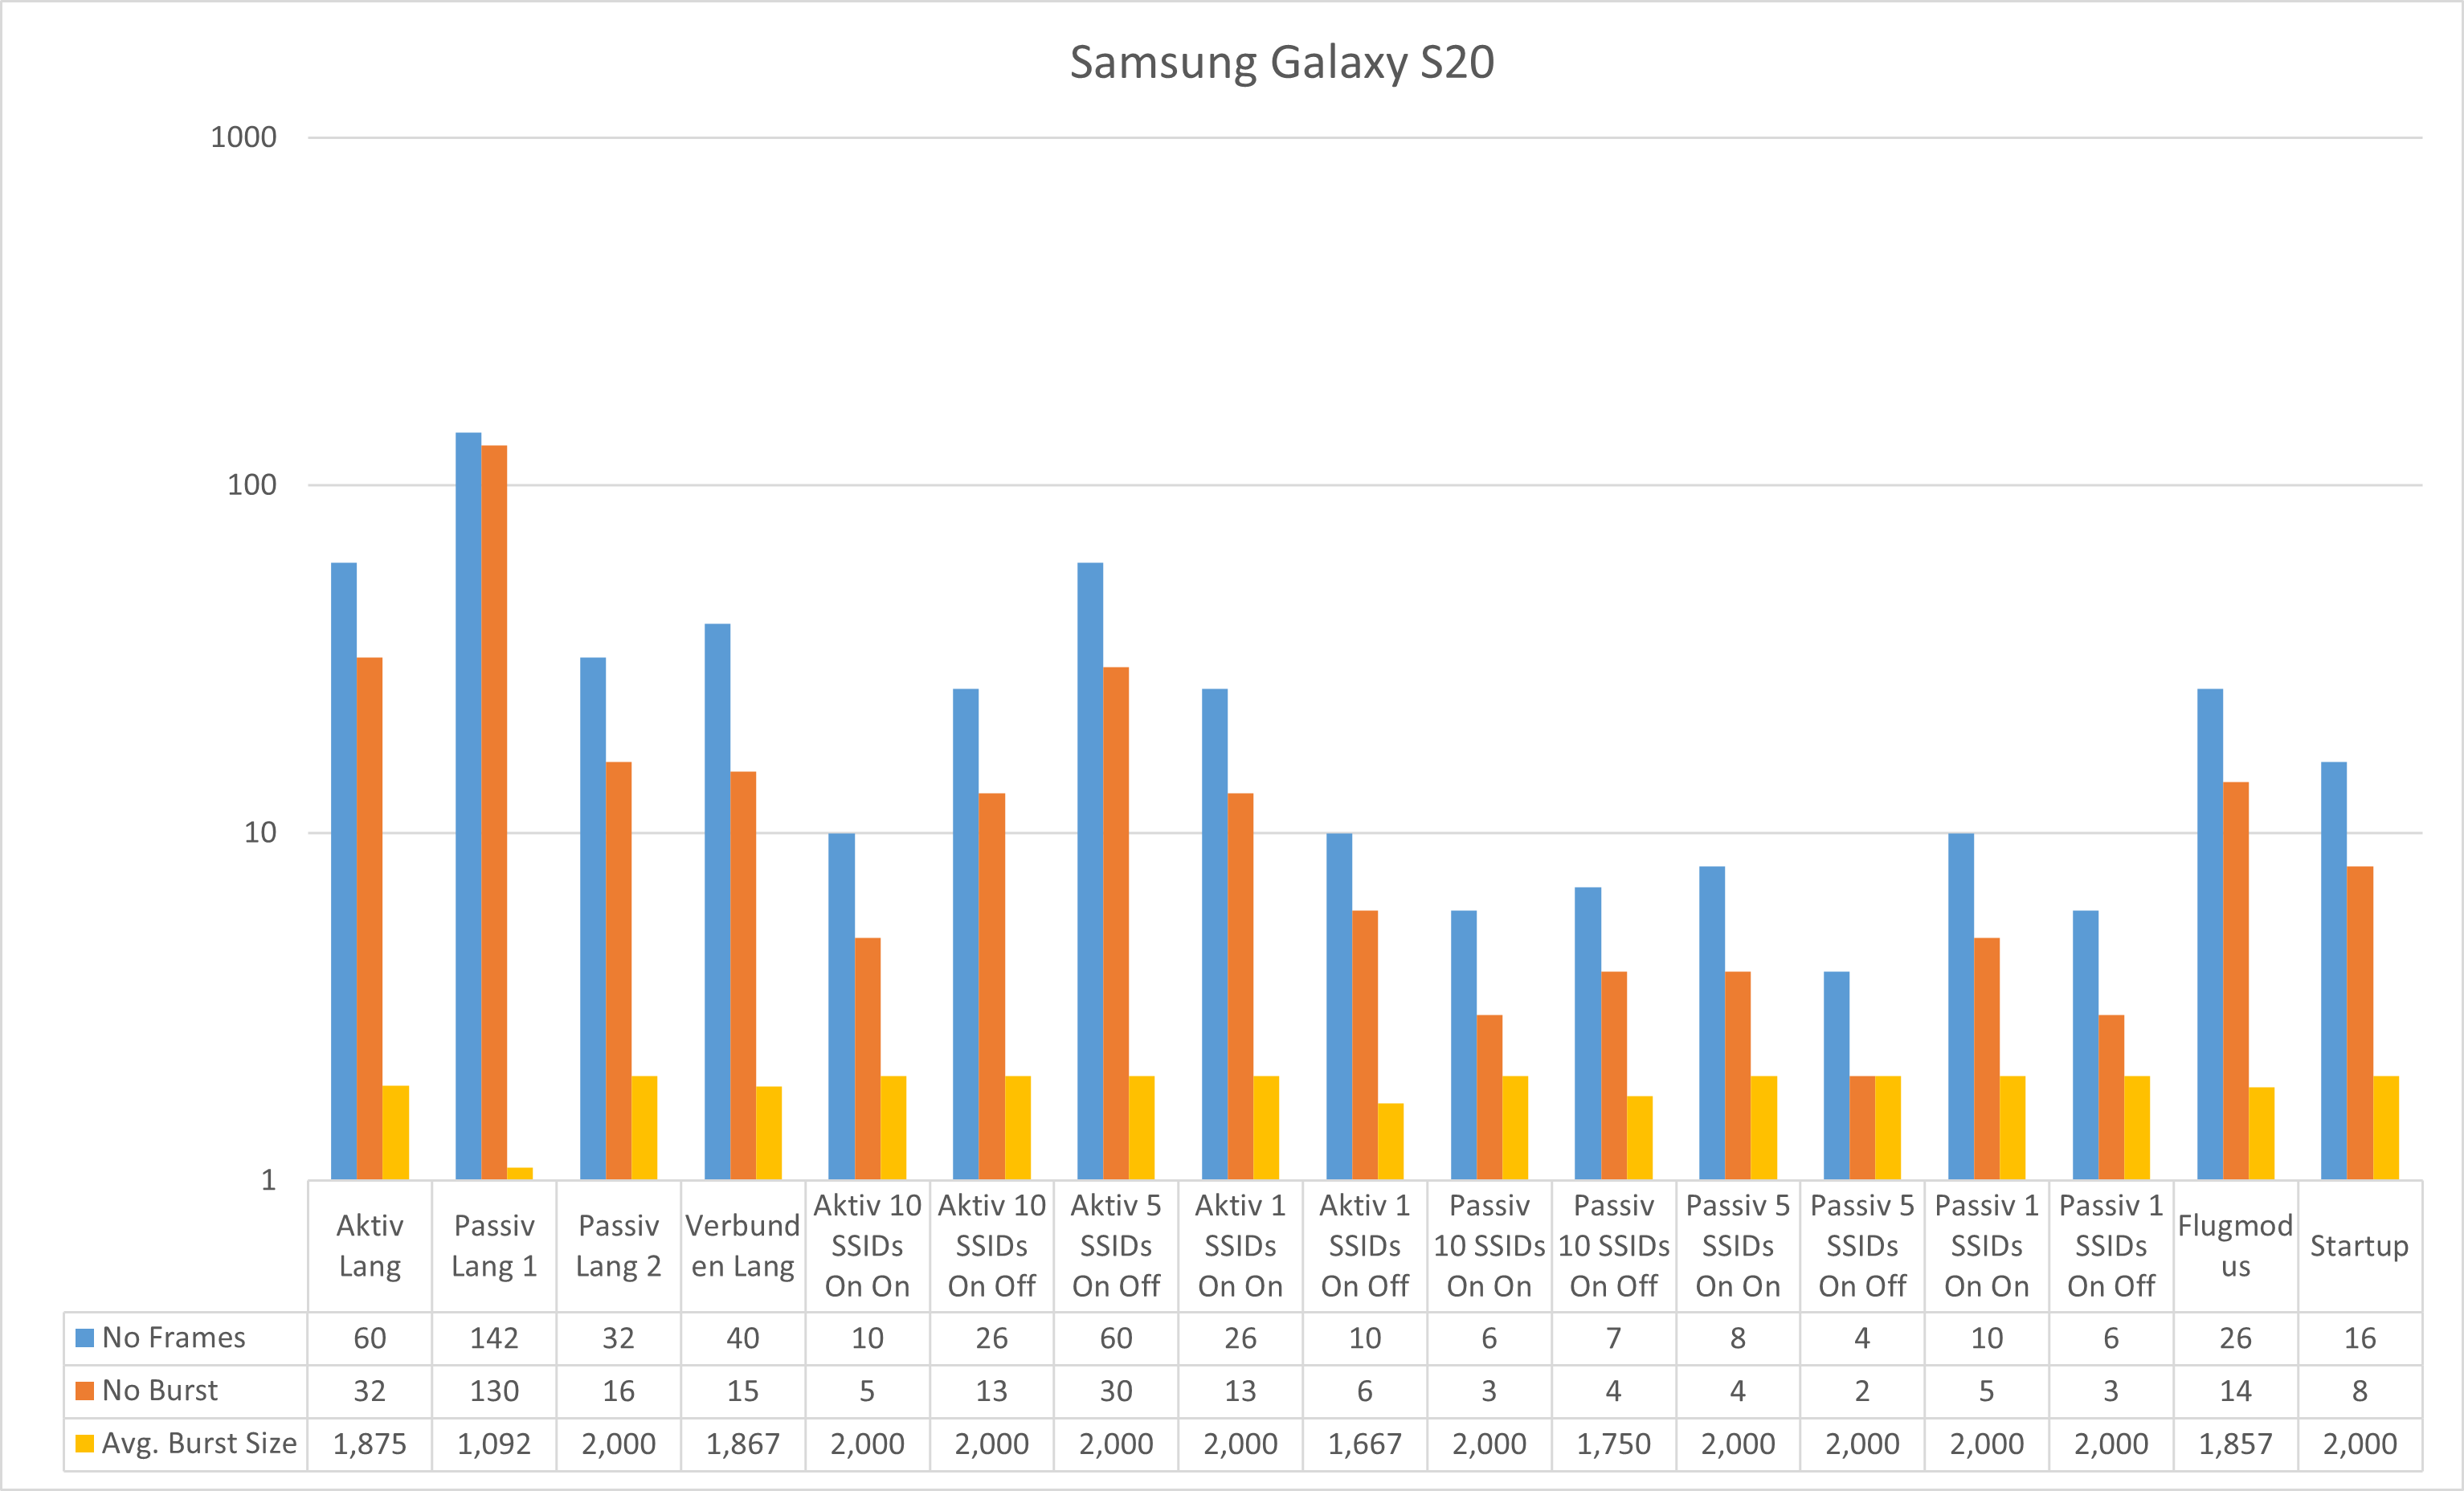
\includegraphics[width=1\linewidth]{Experiments/S20-10.png}
    \caption{Messergebnisse Samsung Galaxy S20 - Android 10}
    \label{figure:androidmeasurementsbycategorys20}
\end{figure}

\clearpage

\begin{figure}[h!]
    \centering
    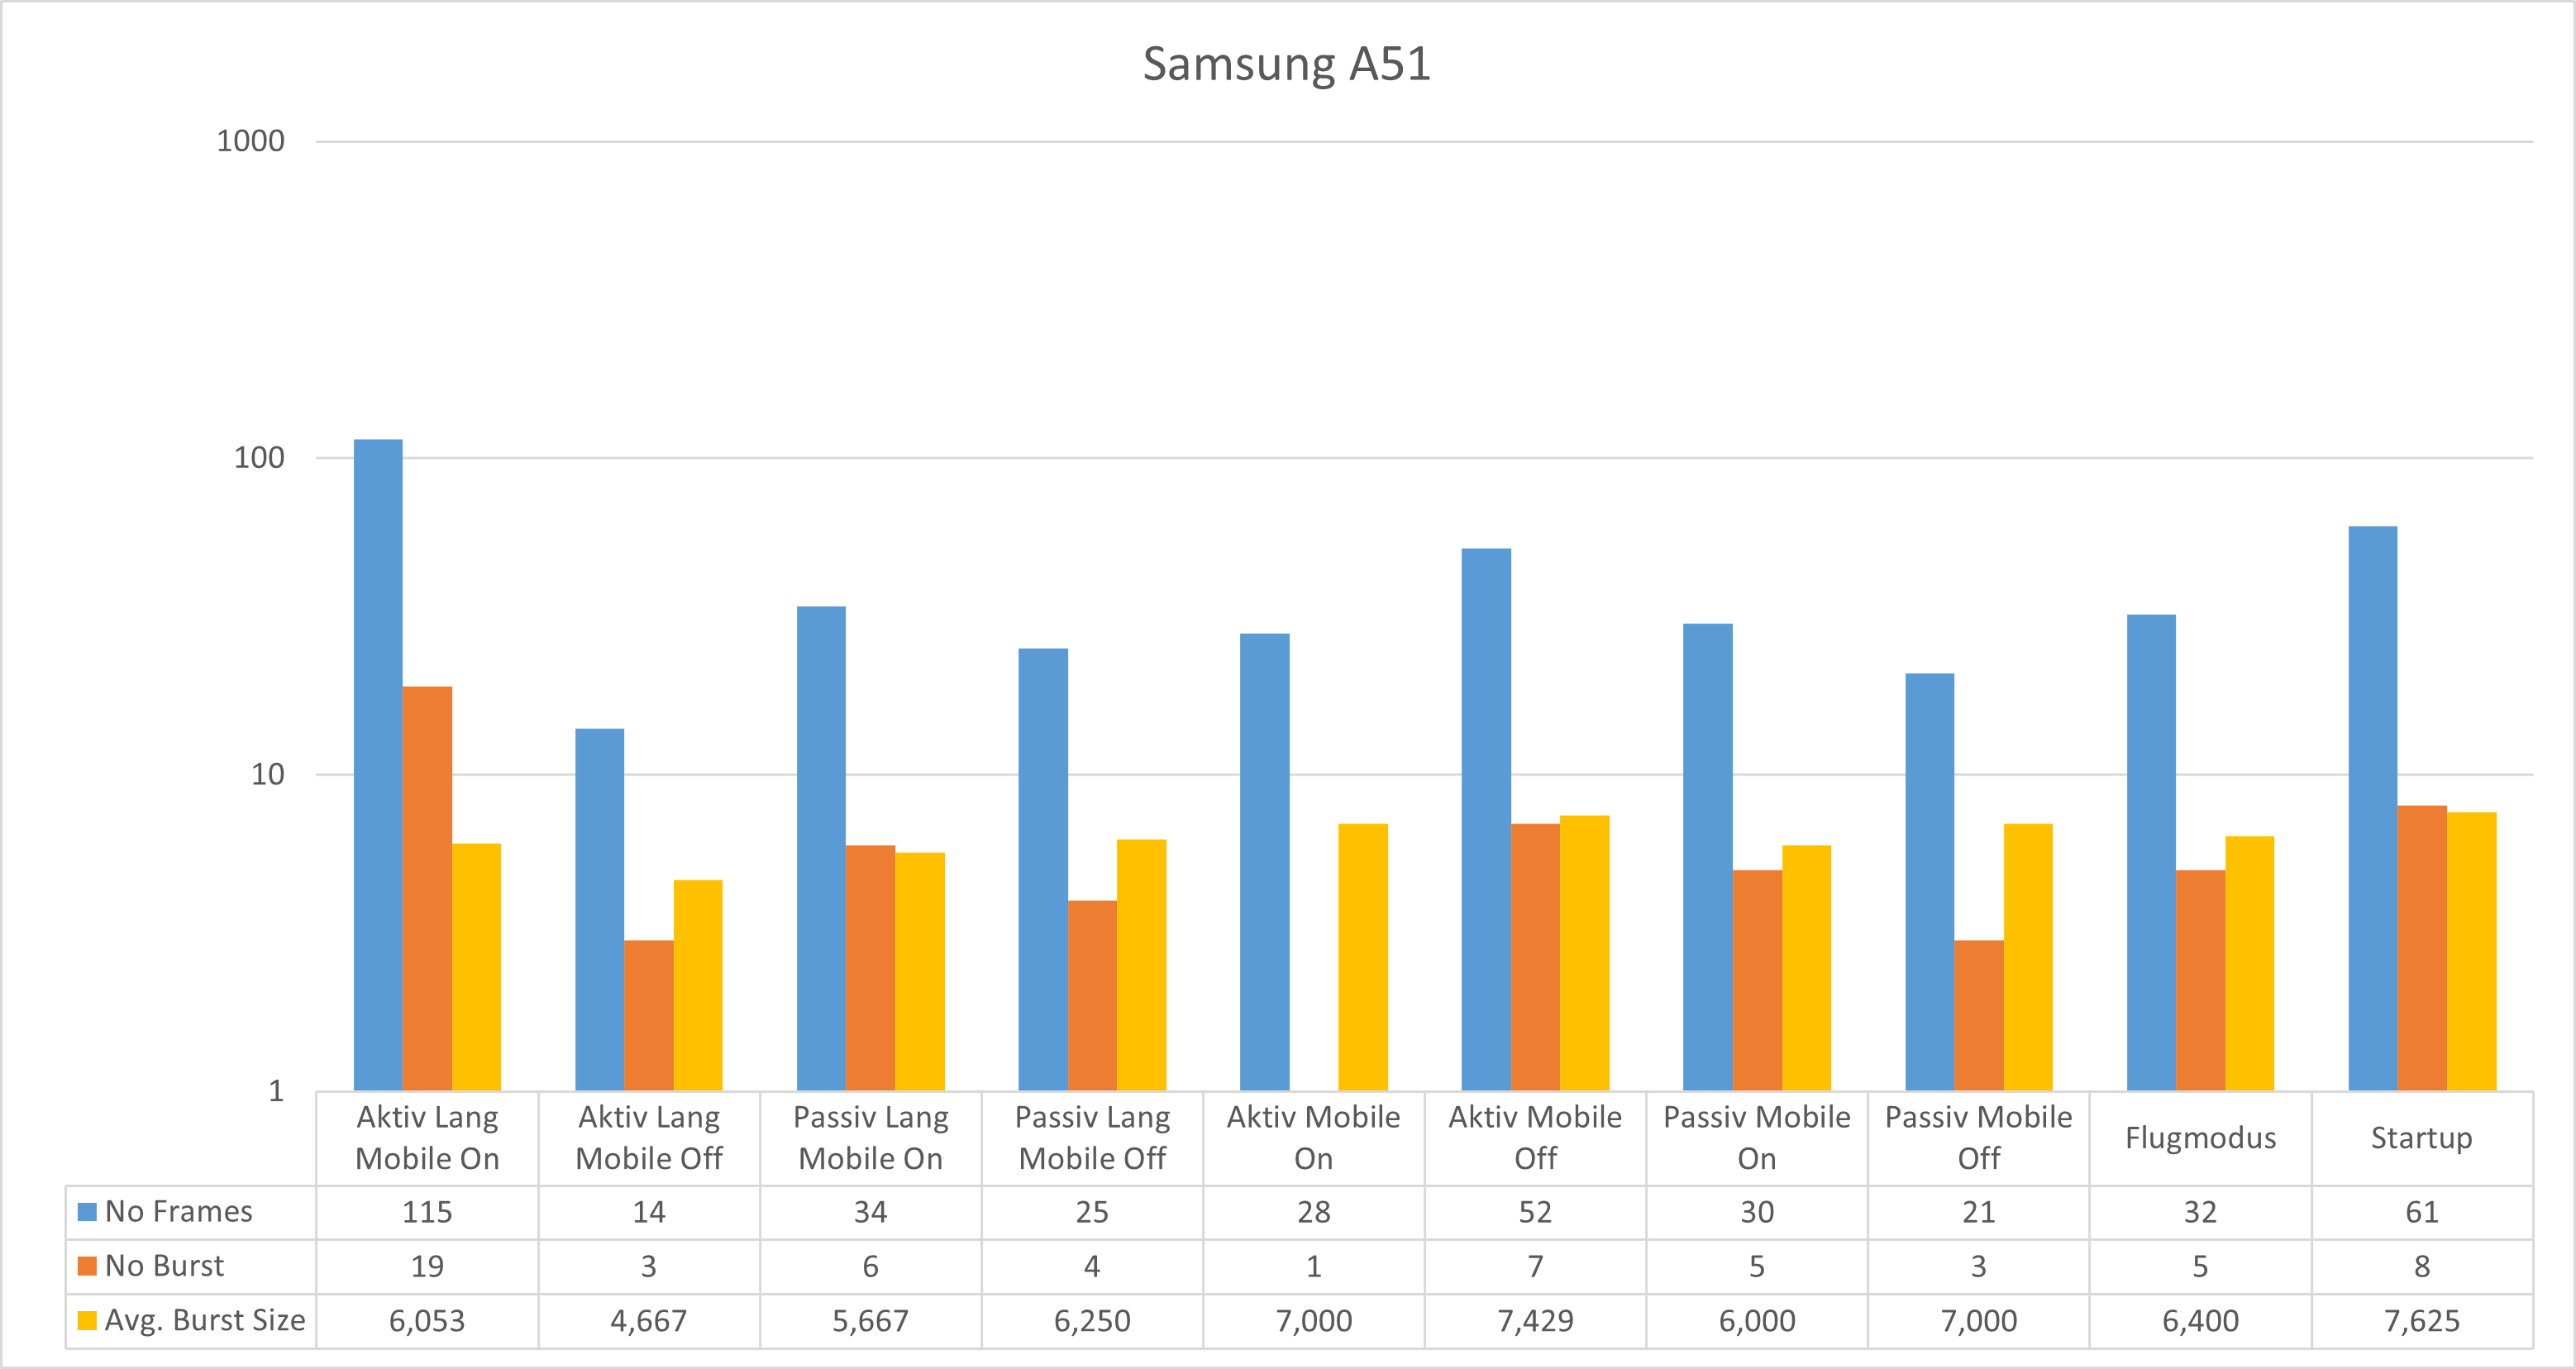
\includegraphics[width=1\linewidth]{Experiments/A51-10.png}
    \caption{Messergebnisse Samsung A51 - Android 10}
    \label{figure:androidmeasurementsbycategorya51}
\end{figure}

Besonders interessant bei der Messung des A51 ist die Tatsache, dass 
das Gerät für alle Messungen immer die MAC-Adresse "02:00:00:00:00:00"
verwendet hat. Lediglich in den Startup- und Flugmodus-Messungen sind 
weitere Probe-Requests mit zufällig generierten MAC-Adressen versendet worden.

\clearpage

\begin{figure}[h!]
    \centering
    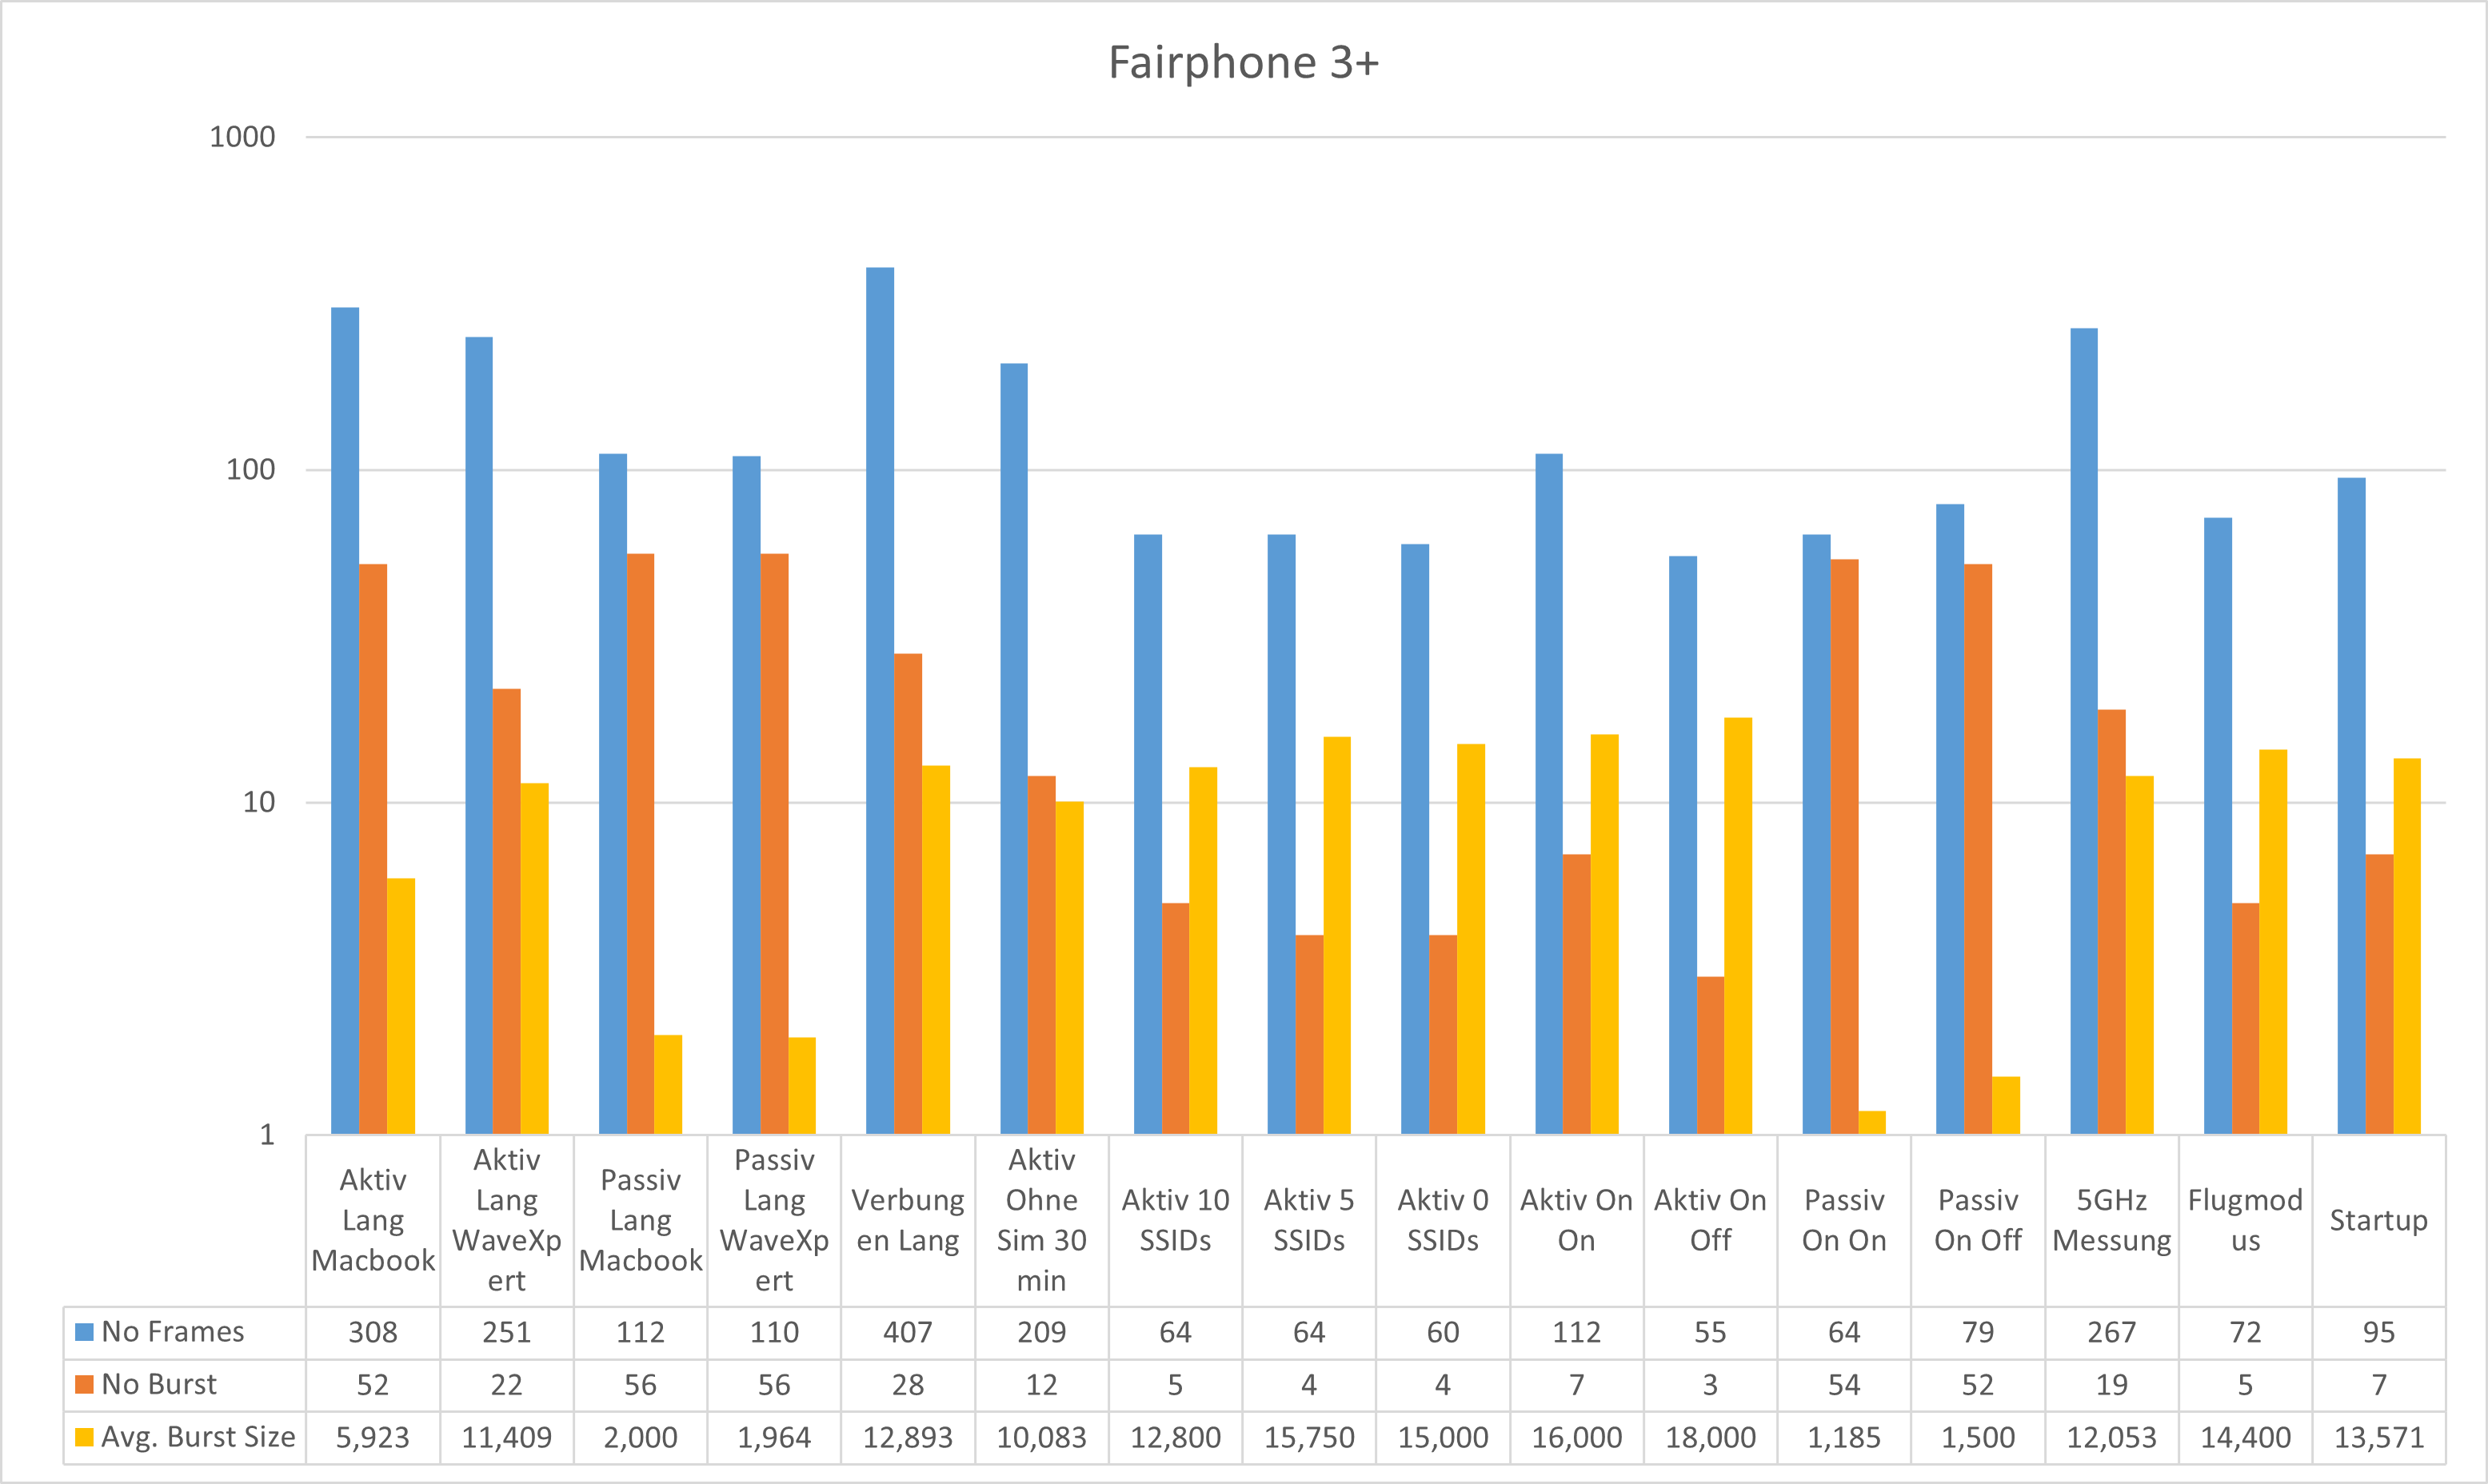
\includegraphics[width=1\linewidth]{Experiments/Fairphone3-10.png}
    \caption{Messergebnisse Fairphone 3+ - Android 10}
    \label{figure:androidmeasurementsbycategoryfairphone}
\end{figure}


Das Fairphone 3+ fällt dadurch auf, dass für die passiven Probe-Requests eine
MAC-Adresse mit Google-OUI und zufälliger NIC verwendet wird. Weiterhin 
ist die Zwischenankunftszeit bei passiven Probe-Request Bursts immer um die 
$63 s$. 

Die Messungen mit dem Fairphone wurden alle mit dem WaveXpert durchgeführt
und es ist in den aufgezeichneten Ergebnissen sehr gut ersichtlich, dass
das Fairphone jeweils einen Burst Probes auf einem Kanal absendet, danach 
den Kanal wechselt und dort die nächste Gruppe Probe-Requests aussendet. 

\begin{figure}[h!]
    \centering
    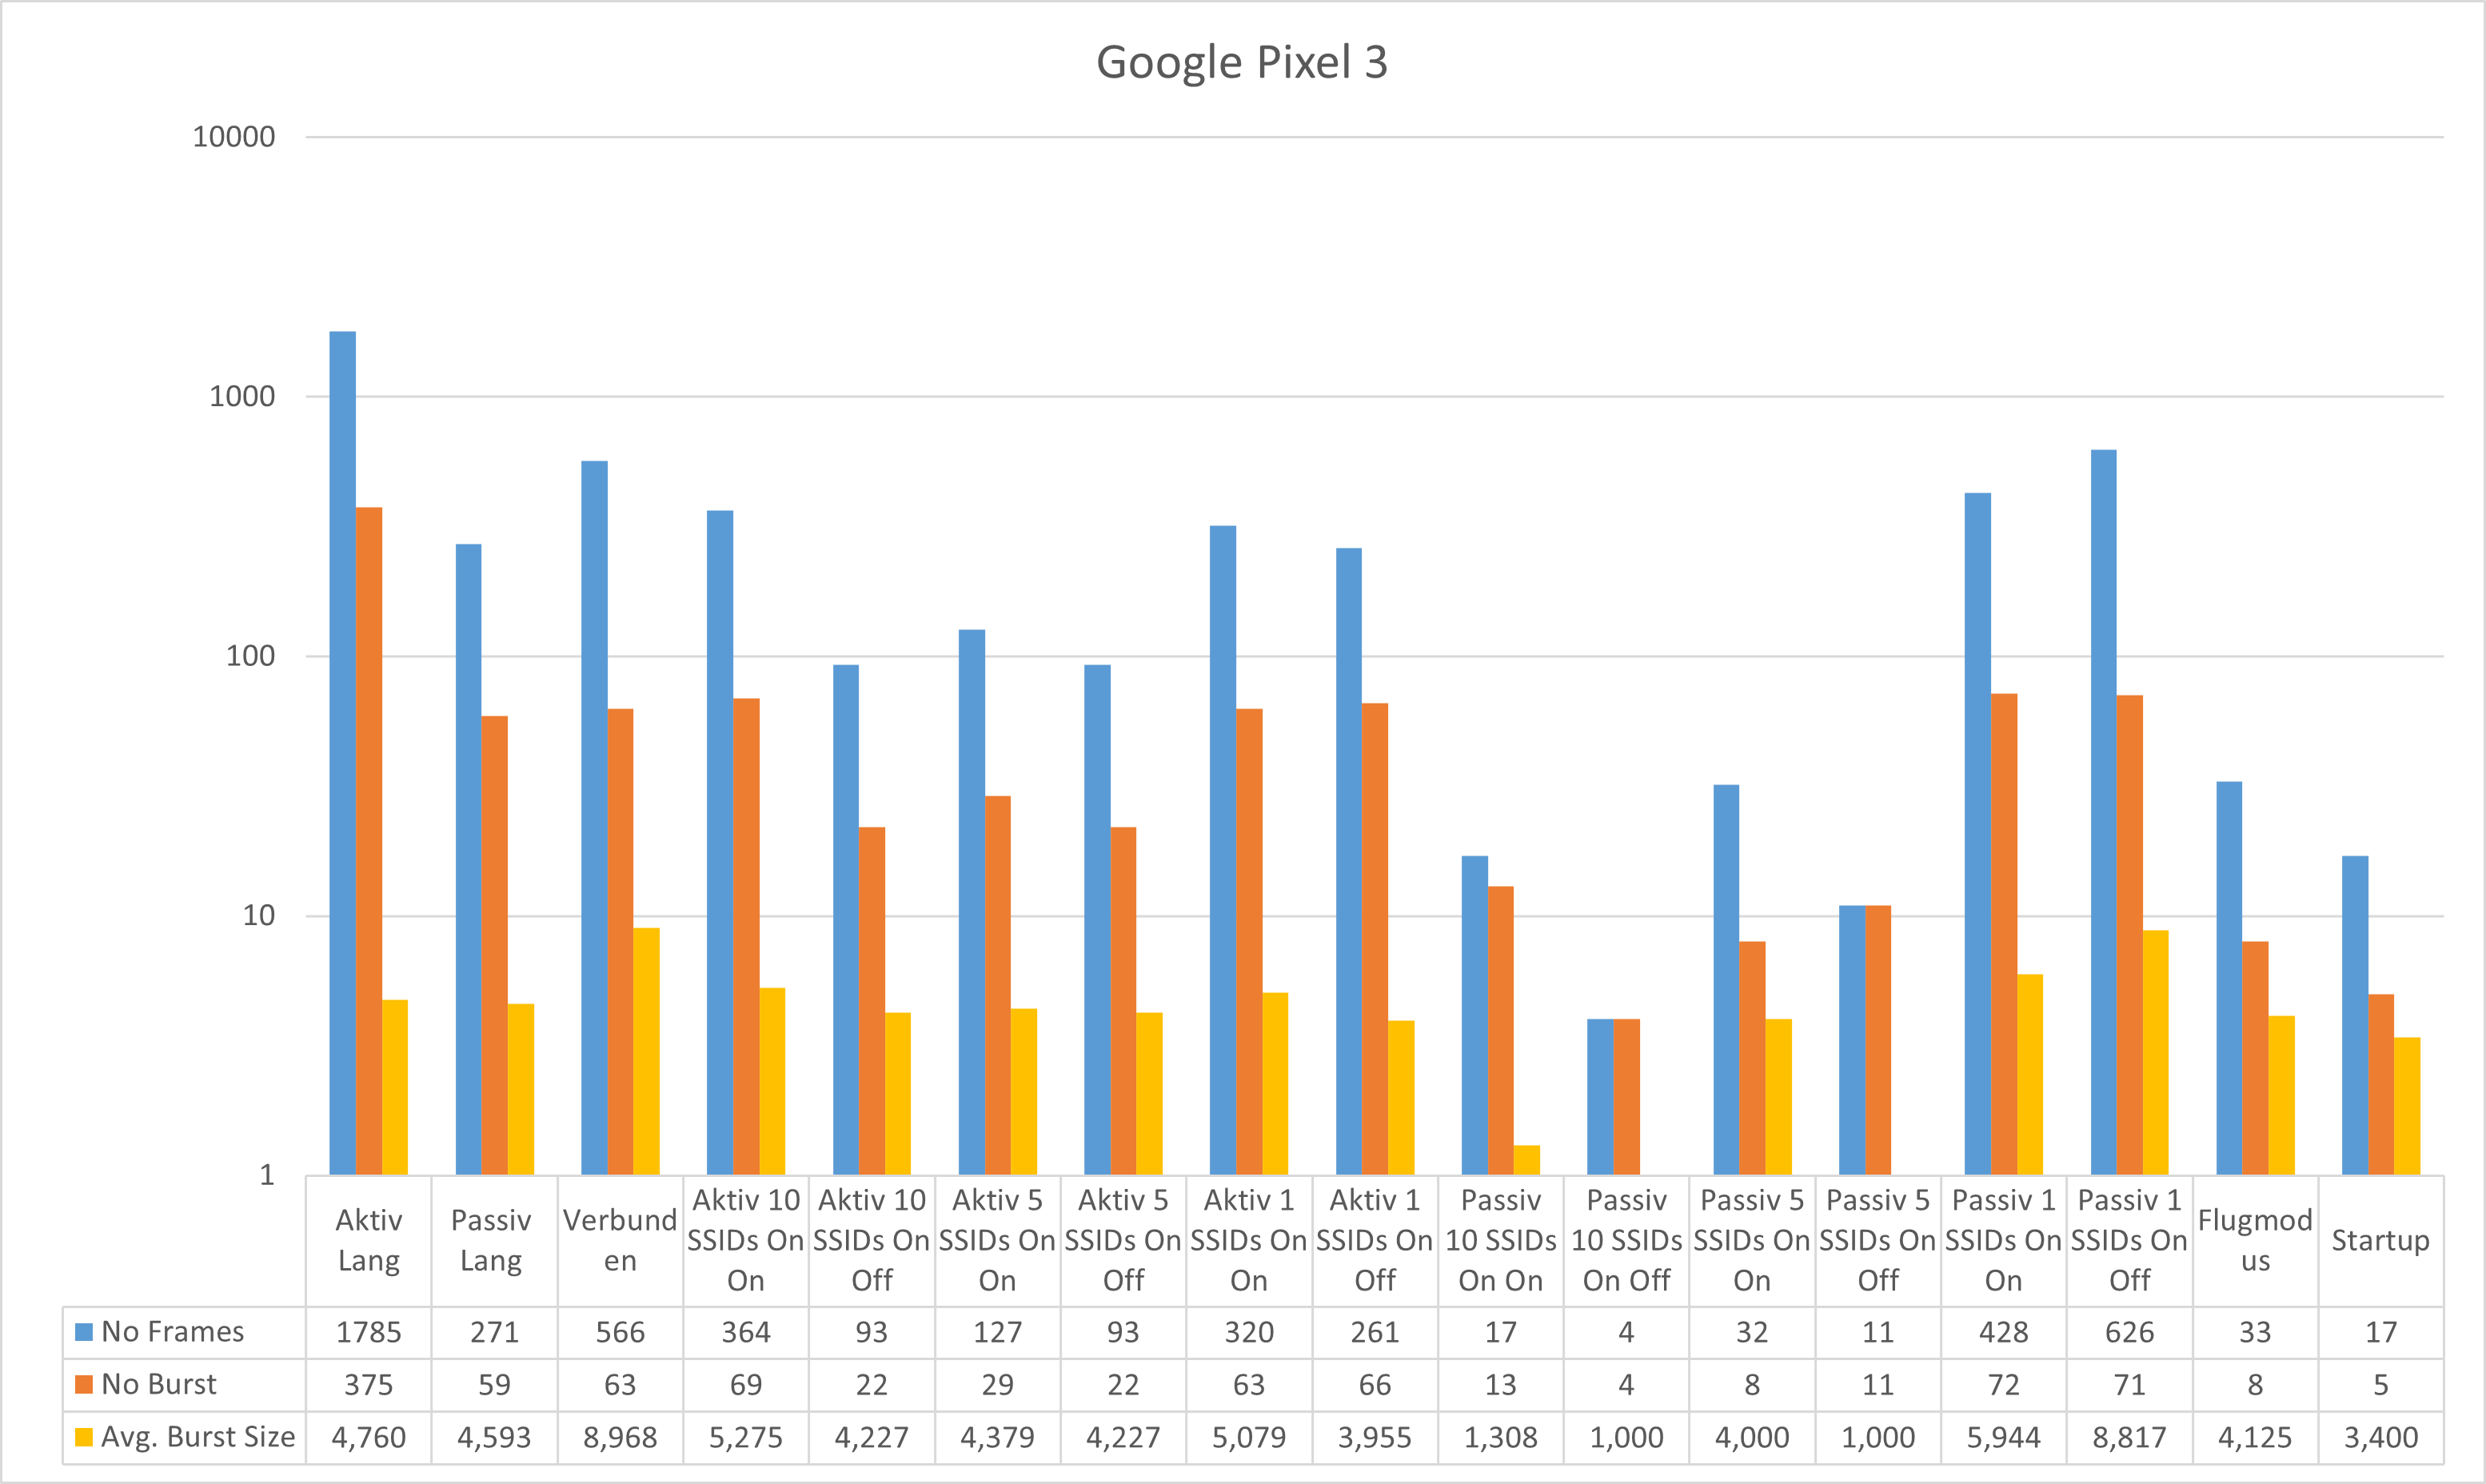
\includegraphics[width=1\linewidth]{Experiments/Pixel3-11.png}
    \caption{Messergebnisse Google Pixel 3 - Android 11}
    \label{figure:androidmeasurementsbycategorypixel}
\end{figure}

\clearpage

\subsubsection*{Erkenntnisse aus den Android-Messungen}
In total $9016$ aufgezeichneten Probe-Requests sind im Schnitt jeweils $5.52$ 
Frames pro Burst mit einer durchschnittlichen Zwischenankunftszeit von $118.24 s$
gemessen worden. Die Bursts beinhalten zwischen einem und 25 Frames.

Mit $4328$ geschätzten verpassten Frames haben Android-Geräte weniger verpasste
Frames relativ zu den aufgezeichneten Frames, was in den Messungen mit dem 
WaveXpert darauf zurückgeführt werden kann, dass Android Geräte die Frames 
pro Kanal gruppiert aussenden. Anders ausgedrückt, ein Android-Gerät sendet 
zuerst einige Frames auf einem Kanal aus, wechselt dann den Kanal und sendet
die nächste Gruppe. Der Vorgang wiederholt sich bei jedem Burst.

Bei genauerer Betrachtung der pcap oder JSON-Dateien zu den einzelnen Messungen
fällt auf, dass Android-Geräte IE-Felder gem. den Tabellen~\ref{table:androidcommoniefields}
und~\ref{table:androidvendorspecificiefields} beinhalten.


\begin{table}[h!]
    \centering
    \begin{tabular}{|c|c|c|c|c|}
        \hline
        \textbf{Tag-NR} & \textbf{0} & \textbf{1} & \textbf{50} & \textbf{3} \\
        \textbf{Tag-Name} & \textbf{SSID} & \textbf{Supported Rates} & \textbf{Ex. Supp. Rates} & \textbf{DS Params Set} \\
        \hline 
        Geräte & alle & alle & alle & alle \\
        \hline
    \end{tabular}
    \caption{IE-Felder, die in allen Messungen vorkommen
    \label{table:androidcommoniefields}}  
\end{table}
Die einzige Ausnahme davon ist das Fairphone 3 welches in den Passivmessungen den 
DS Parameter Set Tag nicht verwendet.

Der in den iOS-Messungen gängige Tag Interworking (107) wird bei Android-Geräten 
nicht verwendet. Dieser Tag kann somit in einem Fingerprinting für die Unterscheidung
von Android- und iOS-Geräten verwendet werden.

Weiterhin verwendet das Google Pixel 3 die HT Capabilities nur im verbundenen Zustand
und die Extended Capabilities gar nicht. Das Fairphone 3 verwendet die Extended Capabilities
auch nie und die HT-Capabilities nur im Passiven Zustand.

\clearpage

\begin{table}[h!]
    \centering
    \begin{tabular}{|c|c|c|c|c|}
        \hline
          & \textbf{Microsoft Corp.} & \textbf{Broadcom} & \textbf{Epigram, Inc} & \textbf{Wi-Fi-Alliance}\\
        \hline 
        A51 & x & & & \\
        Galaxy S8 One & x & x & x & \\
        Galaxy S8 Two & x & x & x & \\
        Galaxy S8 Three & x & x & x & \\
        Galaxy S8 Four & x & x & x & \\
        Galaxy S9 & x & x & x &  \\
        Galaxy S20+ & x & x & x & x \\
        Google Pixel 3 & x & & & x \\
        Fairphone 3+ & x & & & \\ 
        \hline
    \end{tabular}
    \caption{Herstellerspezifische Felder (Vendor Specific - 221)
    \label{table:androidvendorspecificiefields}}  
\end{table}
Auch der Vendor Specific Tag mit der Apple-OUI wird in Android-Geräten nie verwendet
und kann für ein Fingerprinting verwendet werden.

In allen Android Geräten ist das Local Bit gesetzt, was in einem Fingerprinting für eine
zusätzliche Unterscheidung von Android und iOS Geräten genutzt werden kann.

Das Samsung A51, das Fairphone 3+ und die Galaxy S8 haben über mehrere Bursts 
hinweg aufsteigende Sequenznummern.

\subsubsection*{Vergleich mit den MAC-Adressen der Vorarbeit}
In der Vorarbeit wurde eine Tabelle mit den häufigsten auftretenden OUI's von
MAC-Adressen erstellt. Die in dieser Arbeit gemessenen Adressen wurde mit der
Tabelle der Vorarbeit verglichen, um allenfalls Muster zu erkennen. 
Die OUIs der Vorarbeit sind in der Tabelle~\ref{table:commonouis} abgebildet.
CSV-Listen mit den MAC-Adressen aus den Messungen sind im Repository im 
Ordner "Experimente" zu finden.

Es wurden keine Übereinstimmungen der MAC-Adressen aus den Messungen mit den 
OUIs der Vorarbeit gefunden.

\clearpage
\section{Schlussfolgerungen
\label{section:conclusions}}
Anhand der in den Abschnitten~\ref{section:iosmeasurements} 
und~\ref{section:androidmeasurements} genannten Resultate lassen sich nun 
mehrere Verfahren für eine Unterscheidung von Mobilgeräten herleiten.

Hier gilt zu erwähnen, dass die durchgeführten Messungen in dieser Bachelorarbeit
statistisch nicht signifikant sind, da lediglich für das Samsung Galaxy S8 
Tests auf mehr als zwei unterschiedlichen Geräten durchgeführt wurden.
Dies Bedeutet, dass eine Beobachtung, die spezifisch auf einem Gerät gemacht 
wurde, (z.B. Die hauptsächliche Verwendung der MAC-\\Adresse "02:00:00:00:00:00" 
auf dem Samsung A51) nicht für alle Geräte dieses Typs gelten müssen.
Verfahren, die ein Mobilgerät aufgrund der spezifischen Eigenschaften dieses 
Geräts erkennen, können in der Praxis daran scheitern, dass das zu Messende
Gerät sich anders verhält als andere Geräte der selben Bauart.

Trotzdem wurden einige Beobachtungen gemacht, die es in Kombination mit den im 
Kapitel~\ref{chapter:analysis} recherchierten Geräteverhalten ermöglichen,
Mobilgeräte unterschiedlicher Bauart voneinander zu unterscheiden.

\clearpage

\subsection{Generelle Ansätze für ein Fingerprinting anhand ausgesendeter Probe-Requests}
Allgemein kann ein Mobilgerät anhand einer oder mehrerer Eigenschaften von 
anderen Geräten eindeutig unterschieden werden. Kann diese Unterscheidung 
mehrmals nacheinander durchgeführt werden, sind diese Eigenschaften oder eine 
Kombination davon für dieses Gerät einzigartig und dienen somit als Fingerabdruck.
Bevor die MAC-Adresse von Mobilgeräten zufallsgeneriert wurde, 
konnte diese Adresse als Fingerprint genutzt werden. 
Die Abbildung~\ref{figure:naivefingerprinting} zeigt dabei konzeptionell, 
wie solch ein Fingerprinting durchgeführt werden könnte.

\begin{figure}[h!]
    \centering
    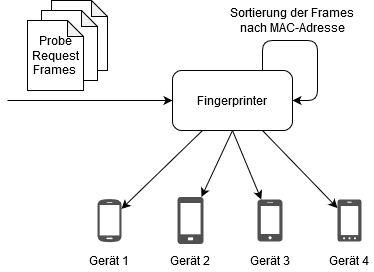
\includegraphics[width=0.8\linewidth]{Experiments/MAC-Fingerprinting.png}
    \caption{Fingerprinting vor iOS 8 / Android 9
    \label{figure:naivefingerprinting}}
\end{figure}

Da die MAC-Adresse in modernen Geräten mit aktuellen Betriebssystemen aber
zufallsgeneriert wird, muss dieses Verfahren angepasst werden.
Ziel ist, Eigenschaften zu finden, um Geräte daran zu unterscheiden.
Dabei gibt es verschiedene Ansätze: Machine Learning-Verfahren versuchen, 
automatisiert aus Millionen von Probe-Requests diese Eigenschaften zu finden 
und Geräte dementsprechend zu unterscheiden.

\clearpage

Ein weiterer Ansatz ist es, automatisiert nach vorgegebenen Filterregeln 
Geräte anhand bekannter Eigenschaften zu sortieren. Diese Filterung kann 
in mehreren Teilschritten vorgenommen werden. Zuerst wird anhand einer 
Eigenschaft sämtliche ankommende oder verfügbare Probe-Requests in diverse 
Gruppen unterteilt. Jede dieser Gruppen kann danach mit weiteren Filtern 
in Untergruppen unterteilt werden. Sind alle Filtervorgänge abge-schlossen,
sollten sämtliche Frames einer Gruppe zu einem eindeutigen Mobilgerät gehören.
Der Ansatz ist in der Abbildung~\ref{figure:sophisticatedfingerprinting} 
konzeptionell dargestellt.

\begin{figure}[h!]
    \centering
    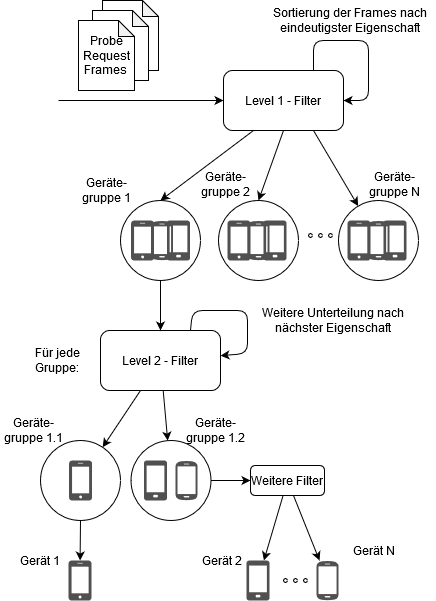
\includegraphics[width=0.8\linewidth]{Experiments/Filter-Fingerprinting.png}
    \caption{Filterbasiertes, hierarchische Geräteunterscheidung
    \label{figure:sophisticatedfingerprinting}}
\end{figure}

\clearpage

Ein Vorteil eines filterbasierten Ansatzes ist, dass neue Erkenntnisse oder 
Änderungen des Geräteverhaltens mit geringem Aufwand implementiert werden können,
indem die Filterregeln dementsprechend angepasst werden. 
Weiterhin muss im Gegensatz zu einem Machine-Learning-Ansatz nicht für jede 
Änderung ein Training des Algorithmus durchgeführt werden (von selbstlernenden
Algorithmen abgesehen). 
Nachteile sind der Aufwand, der benötigt wird, um an die neuen unterscheidbaren
Eigenschaften zu kommen und dass ein Filter-Programm regelmässig 
an die Eigenschaften angepasst werden muss.
Auch hier können selbstlernende Algorithmen eingesetzt werden, um den Aufwand 
zu verringern. 

\clearpage

\subsection{Spezifische Ansätze für die Geräteunterscheidung
\label{subsection:specificapproaches}}
Im Verlaufe der Bachelorarbeit sind mehrere Ansätze entstanden, wie 
eine Unterscheidung von Mobilgeräten durchgeführt werden könnte.
Nachfolgend sind diese Ansätze, deren Vorgehen und die Umsetzbarkeit 
beschrieben.

\subsubsection*{Ansatz 1: Zeitbasierte Auswertung von Frames}
Unabhängig von den Informationen, die in ausgesendeten Probe-Requests enthalten
sind, kann allein aufgrund von zeitlichen Informationen gefiltert werden.
Ein Mobilgerät sendet jeweils einen Burst von Probe-Requests mit der gleichen 
MAC-Adresse aus. Wird innerhalb der Zeit des Bursts ein Frame aufgezeichnet, 
welches eine andere MAC-Adresse hat, wird dieses von einem anderen Gerät 
ausgesendet. 

\paragraph{Vorgehen}
Wenn ankommende Frames in Bursts gruppiert werden, können Frames, die im selben 
Zeitraum aufgezeichnet werden, davon unterschieden werden. 
Allein anhand dieser Information kann eine ungefähre Anzahl von Mobilgeräten 
im Empfangsbereich eines Access-Points evaluiert werden.
Die Abbildung~\ref{figure:timewindowfiltering} beschreibt das Verfahren.

\begin{figure}[h!]
    \centering
    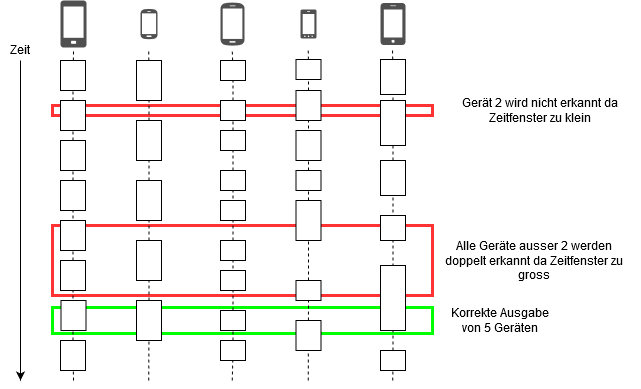
\includegraphics[width=1\linewidth]{Experiments/Zeitfenstermessung.png}
    \caption{Zeitbasierte Filterung von ausgesendeten Probe-Requests
    \label{figure:timewindowfiltering}}
\end{figure}

\clearpage 

Die grösste Schwierigkeit ist dabei, dass das Zeitfenster derart gewählt wird,
dass nicht zwei Bursts eines Geräts als zwei separate Geräte fehlinterpretiert 
werden, oder dass ein Gerät nicht erkannt wird, weil innerhalb des Zeitfensters 
gerade keine Probe-Requests gesendet wurden.
Die Genauigkeit der Messung kann verbessert werden, 
indem mehrere Zeitfenster zu verschiedenen Zeitpunkten ausgewertet werden 
und ein Mittelwert aus den Resultaten gebildet wird.
Zudem kann eine Auswertung der Burst-Zwischenankunfts-zeiten zur Laufzeit 
dazu verwendet werden, das Zeitfenster dynamisch an die Umgebung anzupassen

\paragraph{Umsetzbarkeit}
Dieser Ansatz lässt sich mit wenig Aufwand umsetzen, vorausgesetzt, die 
Probe-Requests werden bereits durch eine Vorfilterung in Bursts aufgeteilt.
Weiterhin ist dieser Ansatz gegenüber einer Veränderung von Geräteverhalten 
robust, da nur die Zwischenankunftszeiten der Bursts für die Unterteilung
benötigt werden.
Allerdings ist die Genauigkeit dieser Filterregel eher gering, da die 
Unterteilung in erster Linie von der Wahl der Dauer des Zeitfensters abhängt. 
Die Messergebnisse zeigen, dass ein Zeitbasierter Ansatz umsetzbar ist, 
da aber die verschiedenen getesteten Geräte keine einheitlichen 
Burstgrössen und -Zwischenankunftszeiten haben, muss die optimale Grösse des 
Zeitfensters experimentell ermittelt werden.

\subsubsection*{Ansatz 2 - Auswertung der Information Element Felder}
Dieser Ansatz beinhaltet zwei Vorgehen:
Zum einen kann aufgrund vorhandener IE-Felder ein Mobilgerät von einem 
anderen unterschieden werden, wenn sie nicht dieselben Felder in ihren 
Probe-Requests verwenden.
Zum anderen können Parameter in diesen Feldern dazu verwendet werden,
Geräte zu unterscheiden.

Der Ansatz wurde auch schon in verwandten Arbeiten angewendet und die 
Messergebnisse lassen darauf schliessen, dass er auch weiterhin für 
ein Fingerprinting verwendet werden kann.

\paragraph{Vorgehen}
Eintreffende Probe-Request werden nach ihren IE-Feldern sortiert und in 
distinkte Gruppen unterteilt. 
Im Idealfall befindet sich pro Gruppe nur ein einzelnes Mobilgerät.
Da gemäss unseren Messergebnissen aber mehrere Geräte die selben IE-Felder 
in ihren Probe-Requests verwenden und die Parameter in diesen Feldern 
auch identisch sein können, werden aber in jeder Gruppe mehrere Geräte auftreten.
Ein weiteres Problem ist die Tatsache, dass ein Mobilgerät in mehreren Bursts
nicht die selben IE-Felder verwenden muss. 
Somit ist es möglich, dass Bursts eines Geräts als mehrere Mobilgeräte erkannt 
werden.

\paragraph{Umsetzbarkeit}
Das Auslesen und Auswerten von Information Element Feldern aus Probe-Requests 
kann mit geringem Aufwand durchgeführt werden.

\subsubsection*{Ansatz 3 - Filtern von nichtrandomisierten MAC-Adressen}
Wird die gleiche MAC-Adresse über mehrere Bursts erkannt, kann davon ausgegangen 
werden, dass das Gerät die MAC-Adresse nicht randomisiert. In diesem Fall kann
eine Filterung gemäss der Abbildung~\ref{figure:naivefingerprinting} durchgeführt
und die MAC-Adresse des Geräts als Fingerabdruck verwendet werden.

\paragraph{Vorgehen}
Parallel zu anderen Filtern kann die wiederholte Verwendung von MAC-Adressen über
mehrere Bursts erkannt werden. Weitere Bursts mit dieser Adresse können direkt 
mit dem Fingerabdruck versehen werden.

\paragraph{Umsetzbarkeit}
Wenn bereits eine Gruppierung von Probe-Requests nach Bursts vorgenommen wurde,
benötigt die Umsetzung dieses Verfahrens nur geringen Aufwand.

\subsubsection*{Ansatz 4 - Filterung zur Laufzeit anhand Burst-Zwischenanktunftszeiten}
Wenn für sämtliche Gerätetypen und Betriebssysteme die Zwischenankunftszeiten
bekannt ist, und diese sich deterministisch verhalten, ist es möglich, 
eintreffende Bursts anhand dieser Zeiten einem bekannten gerät zuzuordnen.

\paragraph{Vorgehen}
Angenommen, man hat ein Mobilgerät, welches immer 30 Sekunden nach dem 
letzten Probe-Request einen neuen Burst aussendet. 
Somit spielt es keine Rolle, ob die MAC-Adresse in jedem Burst neu 
zufallsgeneriert wird, da man nach einer Messung nur die 30s wartet und 
den neuen Burst für den Fingerprint aktualisiert.

Dieses Vorgehen hat mehrere Schwächen:
\begin{itemize}
    \item Falls ein Mobilgerät die Bursts nicht immer in gleichbleibenden 
    Abständen aussendet, lässt sich das Verfahren nicht anwenden.
    \item Wenn zwei Mobilgeräte dieselbe Zwischenankunftszeit haben, 
    können diese nicht unterschieden werden.
    \item Wenn ein Mobilgerät eine Verzögerung von 30s und ein weiteres 
    Mobilgerät eine Verzögerung von 15s haben, 
    kann man diese Geräte alle 30 Sekunden nicht unterscheiden.
    \item Wenn zwei Probe-Requests von unterschiedlichen Mobilgeräten 
    zur gleichen Zeit aufgezeichnet werden, 
    lassen sich die Mobilgeräte nicht unterscheiden

\end{itemize}

\paragraph{Umsetzbarkeit}
In den Versuchen hat sich herausgestellt, dass die meisten Geräte die 
Bursts in zufälligen Zeitintervallen aussenden. 
Somit lässt sich dieses Verfahren nicht generell umsetzen.
In Kombination mit anderen Verfahren kann dieser Ansatz aber dazu verwendet 
werden die Genauigkeit dieser Verfahren zu erhöhen. 
Dazu muss zur Laufzeit ausgewertet werden, ob die Zwischenanktunftszeiten 
von Bursts eines Gerätes deterministisch sind, bevor künftige Probe-Requests 
danach sortiert werden.

\subsubsection*{Ansatz 5 - Bitweise MAC-Header-Analyse}
Im Paper "Noncooperative 802.11 MAC Layer Fingerprinting and Tracking 
of Mobile Devices” aus dem Jahr 2017 wird ein Verfahren beschrieben, 
mit dem ein Fingerprinting und Tracking bewerkstelligt werden könnte.

\paragraph{Verfahren}
Prinzipiell wird jedes Bit des Probe-Request MAC-Headers mittels der 
Berechnung der Entropie über sämtlichen vergangenen Messungen gewichtet. 
Neu auftretende Felder oder selten verwendete Felder haben eine hohe Gewichtung 
und werden für ein Fingerprinting direkt verwendet. 
Felder, die in einer Vielzahl von Probe-Requests vorkommen, 
werden für den Fingerprint ignoriert.

\paragraph{Umsetzbarkeit}
Im Vergleich mit den bisher genannten Verfahren ist dieser Ansatz der 
Aufwändigste und wird voraussichtlich im Rahmen dieser Arbeit nicht umgesetzt.

\subsubsection*{Ansatz 6 - Filterung nach Sequenznummer}
Für Geräte, deren Sequenznummer nicht pro Burst zufallsgeneriert wird,
können Bursts daran erkannt werden, dass die Sequenznummer in neueren 
Frames inkrementiert wird.

\paragraph{Verfahren}
Wird erkannt, dass ein Mobilgerät in mehreren aufeinanderfolgenden 
Bursts die Sequenznummer nicht zufallsgeneriert, 
kann diese Erkenntnis dafür genutzt werden, 
eine Unterscheidung von Mobilgeräten genauer zu machen.
Wenn Beispielsweise mit einem anderen Verfahren die Unterscheidung 
von zwei Bursts nicht möglich ist, aber erkannt wurde, 
dass Gerät A die Sequenznummer nicht randomisiert 
(unabhängig ob B ebenfalls die Sequenznummer nicht randomisiert), 
kann man denjenigen Burst auswählen, dessen Sequenznummer näher an der des 
vorhergehenden Bursts ist.

\paragraph{Umsetzbarkeit}
Die Versuche haben gezeigt, dass mehrere Geräte die Sequenznummern nicht 
für neue Bursts zufallsgenerieren.
In Kombination mit anderen Verfahren bietet diese Lösung eine 
Möglichkeit die Genauigkeit einer Unterscheidung zu erhöhen.

\subsubsection*{Ansatz 7 - Filterung nach Framelänge}
Wenn ein Gerät bei den Probe-Requests immer die gleiche Frame Länge hat, 
können die Probe-Requests dieses Gerätes daran erkannt und von Probes von 
anderen Geräten unterschieden werden.

\paragraph{Verfahren}
Dieses Verfahren ist vom Prinzip her ähnlich wie die Erkennung der IE Felder. 
Es ist allerdings einfacher, ein Frame anhand der Länge, 
die in Wireshark spezifisch ausgegeben wird, zu kategorisieren.

\paragraph{Umsetzbarkeit}
In den Messungen wurde erkannt, dass die Frame-Länge je nach dem messenden 
Gerät unterschiedlich sein kann, 
da abhängig von der Netzwerkkarte unterschiedliche Radiotap Header-Informationen 
aufgezeichnet werden. 
Deshalb wird dieses Verfahren nicht umgesetzt und stattdessen die Filterung nach 
IE-Feldern implementiert.

\subsubsection*{Ansatz 8 - Filtern nach Local-Bit}
Wenn ein Mobilgerät für sämtliche Frames in der zufallsgenerieren MAC-Adresse
das Local-Bit immer setzt, kann dieses Gerät von einem anderen Gerät, 
welches das Local-Bit auch zufällig setzt, unterschieden werden.

\paragraph{Verfahren}
Ähnlich wie in den Verfahren 3 und 6 kann zur Laufzeit evaluiert werden,
ob in einer Gerätegruppe in den Frames der Bursts das Local Bit immer 
gesetzt ist. Künftig aufgezeichnete Frames können danach herausgefiltert werden.

\paragraph{Umsetzbarkeit}
Auch dieses Verfahren kann in Kobmbination mit anderen Verfahren dazu beitragen,
die Genauigkeit einer Unterscheidung zu verbes-sern.

\clearpage

\part{Prototyp}
\section{Prototyp-Einführung}
In den folgenden Abschnitten wird die Funktionsweise des Prototyps be-schrieben.
Dabei handelt es sich in erster Linie um ein Proof-of-Concept und nicht um eine 
vollumfängliche Softwarelösung. 
Der Prototyp entspricht dabei der im Abschnitt~\ref{section:conclusions} genannten
Lösung mit hierarchisch implementierten Filterregeln, die ankommende Probe-Requests 
in jeder Hierarchiestufe weiter unterteilen. Als Ergebnis entstehen distinkt 
voneinander unterscheidbare Gruppen von Probe-Requests, die potentiell zu einzelnen 
Geräten gehören.

Im Prototyp werden prinzipiell Prozessschritte gemäss folgender Auflistung vorgenommen.
\begin{itemize}
    \item Preprocessing
    \item Vorfilterung
    \item Filterung
\end{itemize}

Bei der Programmierung der Filter wurde darauf geachtet, dass der Input und der Output 
in einem einheitlichen Format gehalten wird. Dieses Vorgehen erlaubt es dem Anwender,
die einzelnen Verfahren in der Reihenfolge auszutauschen und die Ergebnisse untereinander
zu vergleichen und somit eine optimale Reihenfolge festzulegen.
Das gewählte Format ist hierbei ein Python-Dictionary (nachfolgend Dictionary genannt), 
welcher jeweils als Schlüssel-Werte-Paar eine Liste von Bursts beinhaltet.


\subsection{Preprocessing}
Im Preprocessing werden zuerst die einzelnen Probe-Requests aus den JSON-Dateien 
extrahiert und in einzelnen Frame-Klassen instanziert.
Danach werden die Frames anhand der MAC-Adresse in die einzelnen Bursts klassifiziert, 
in Burst-Klassen eingeteilt und als Pyhton-Liste (nachfolgend Liste genannt) gespeichert. 
Die Liste ist dabei aufsteigend nach der Ankunftszeit der Bursts sortiert.
Ein Burst-Objekt hat jeweils die in den Frames verwendete MAC-Adresse, 
die Ankunftszeit des ersten und des letzten Frames, einen Boolean, 
ob das Lokale Bit gesetzt ist und eine Liste von Frames als 
Parameter. Auch die Liste der Frames ist aufsteigend nach der Ankunftszeit der Frames 
sortiert um in weiteren Filterschritten anhand der Ankunftszeit weiter filtern zu können.

\clearpage

\subsection{Vorfilterung}
Die Vorfilterung dient dem Zweck, das Datenset von Bursts zu säubern, die nicht weiter 
gefiltert werden müssen.
Wird in einem Filterforgang festgestellt, dass ein Gerät seine wahre MAC-Adresse 
verwendet, kann diese Adresse in einem Set gespeichert werden und neue ankommende 
Probe-Requests können in der Vorfilterung aus dem Datenset entfernt werden, wenn 
sie eine der MAC-Adressen im Set verwenden. Es können zwei Fälle auftreten, 
in denen Geräte ihre wahre MAC-Adresse verwenden. Erstens, wenn das Gerät seine 
Adresse nicht zufallsgeneriert und zweitens, wenn das Gerät mit einem Acess-Point 
verbunden ist und die randomisierung der MAC-Adresse im verbundenen Zustand
nicht eingestellt hat. Der erste Fall tritt bei älteren Geräten auf, deren 
Betriebssystem eine randomisierung der MAC nicht zulässt oder wenn auf dem Gerät 
die Einstellung, Adressen zufällig zu generieren, nicht eingestellt ist.
Beide Fälle lassen sich daran erkennen, dass ein Gerät über mehrere Bursts hinweg die 
selbe MAC-Adresse verwendet. Es gibt dabei Geräte, die im verbundenen Zustand im SSID-Tag 
die MAC-Adresse des Netzwerks verwenden.

\subsection{Filterung}
Anhand den im Abschnitt~\ref{section:conclusions} genannten Ansätze wurde versucht, 
zwei Filterregeln zu implementierten.
Ziel dieser Filter ist es, Bursts in Gruppen zu unterteilen und diese Gruppen 
so lang weiter zu unterteilen bis potentiell pro Gruppe nur Bursts von einem Gerät 
existieren. 

\subsubsection*{Filtern nach IE-Feldern}
Zuerst werden die Bursts nach den verwendeten Information-Element-Feldern klassifiziert.
In den Messungen wurde festgestellt, dass einzelne Geräte für Probe-Requests merhheitlich
die selben IE-Felder verwenden. 
Die verwendeten IE-Felder werden innerhalb jeder der Listen, 
welche von der Vorfilterung erstellt wurde, 
von Burst zu Burst miteinander verglichen. 
Die Bursts werden dann anhand der IE-Felder in weitere Listen unterteilt und 
zurückgegeben.

\clearpage

\subsection{Verwerfen des Ansatzes zur Zeitbasierten Auswertung
\label{subsection:timefilter}}
Es wurde versucht, das im Unterabschnitt~\ref{subsection:specificapproaches} 
genannte Verfahren für die zeitbasierte Auswertung im Prototypen umzusetzen.
Dabei fiel auf, dass die Dauer eines Bursts (Zeit zwischen dem ersten und 
letzten Frame im Burst) zu kurz ist, um das Verfahren wie geplant anzuwenden.

Selbst Bursts mit mehr als zehn Frames haben eine Dauer von weniger als einer 
Sekunde. Kombiniert mit der unvorhersehbaren Zwischenankunftszeit der Bursts 
ist es unmöglich, ein Zeitfenster zu finden, welches eine genaue Zählung der 
Mobilgeräte ermöglicht.

In einer zusätzlichen Auswertung der Messungen der vier Samsung Galaxy S8 
kann aufgezeigt werden, dass sich selbst identische Gerätetypen mit der 
gleichen Betriebssystemversion sehr unterschiedlich verhalten. 
Das Verhalten wird in der Abbildung~\ref{figure:bursttimeanalysis} dargestellt.

\begin{figure}[h!]
    \centering
    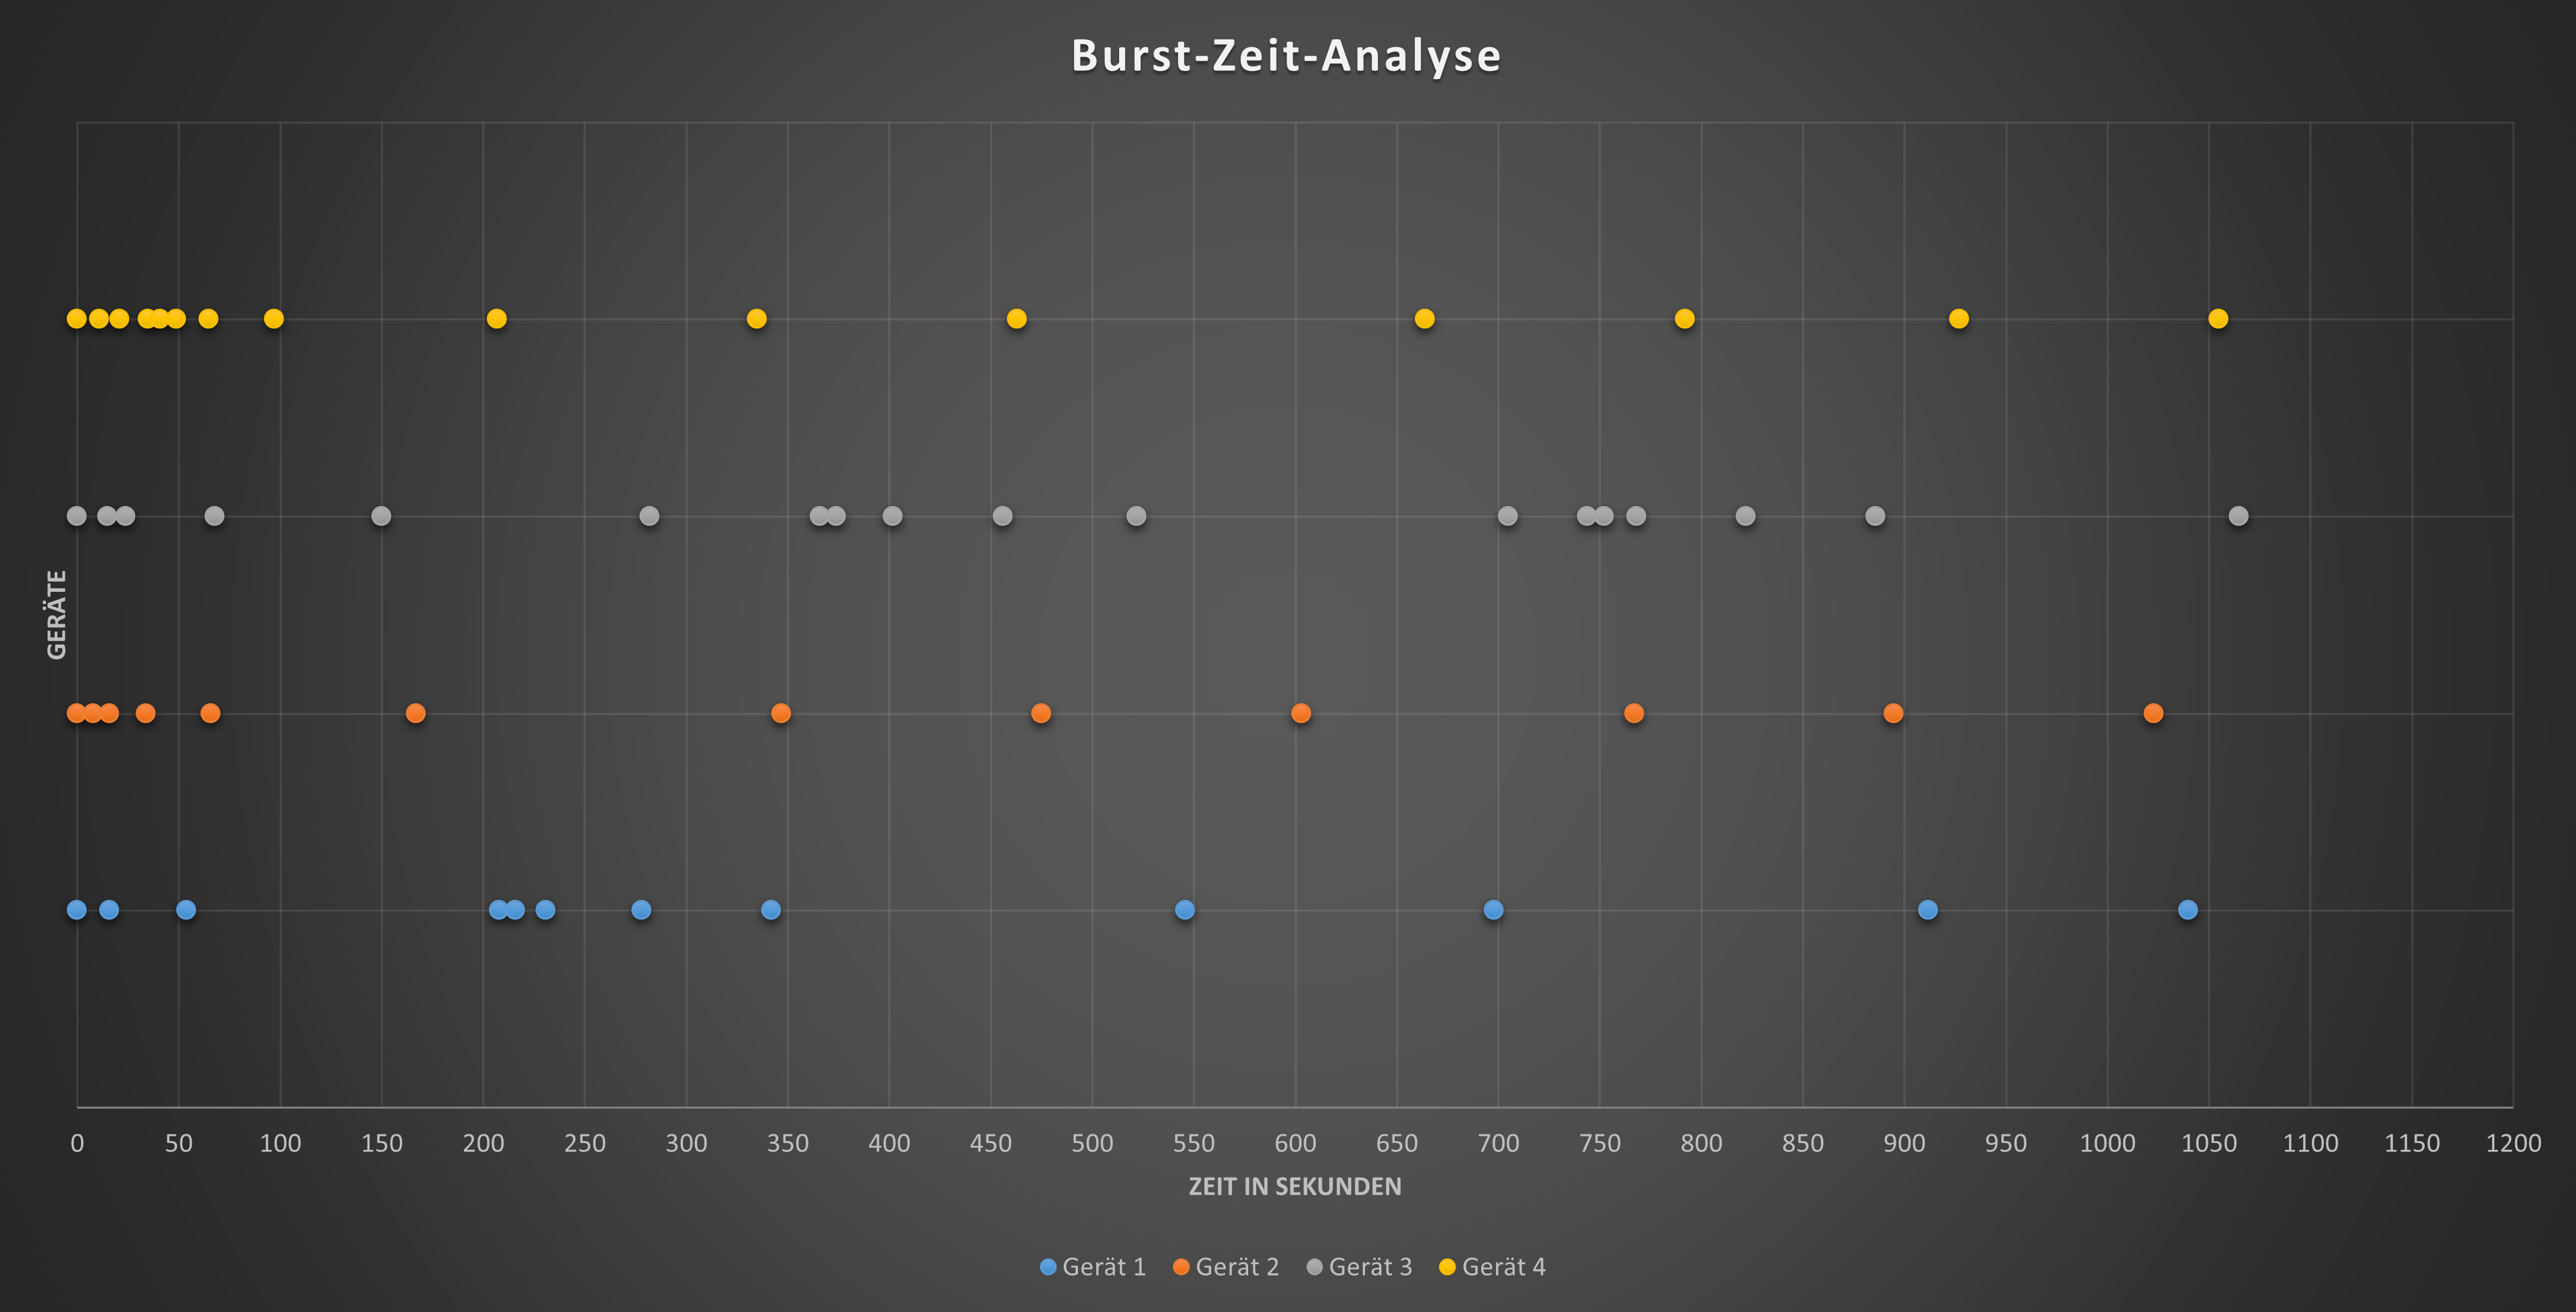
\includegraphics[width=1\linewidth]{Prototype/Burst-Zeit-Analyse.png}
    \caption{Auswertung der Bursts von vier Samsung Galaxy S8 Geräten.
    \label{figure:bursttimeanalysis}}
\end{figure}

Man kann sehr schön erkennen, dass es keine Regelmässigkeit zwischen allen vier 
Geräten gibt. Die Geräte zwei (Orange) und vier (Gelb) verhalten sich ähnlich, 
dadurch dass sie zu Beginn der Messung einige Probe-Requests in kurzer Abfolge 
aussenden und danach die Zwischenankunftszeiten grösser werden.
Das Gerät drei (Grau) scheint die Zwischenankunftszeit der Probe-Requests jeweils 
mit jedem Burst zu erhöhen bis nach ca. 350 Sekunden wieder ein Reset durchgeführt 
wird.
Das Gerät eins (Blau) verhält sich zu Beginn ähnlich wie das Gerät drei, 
wechselt aber zum Zeitpunkt 550 in einen regelmässigen Rithmus.

\clearpage

Wenn man nun als Beispiel den Zeitpunkt 350 betrachtet, kann man sehen, dass 
kurz davor oder danach alle Moblilgeräte Probe-Requests ausgesendet haben. 
Mit einem angenommenen Zeitfenster von 50 Sekunden werden nun alle Bursts 
zwischen den Zeitpunkten 325 und 375 erfasst und es muss entschieden werden,
wie viele Geräte sich im Datenset befinden. Insgesamt werden im Zeitfenster
fünf Bursts erkannt. Jeweils ein Burst gehört zu den Geräten eins, zwei und vier 
und zwei Bursts geören zum Gerät drei. Nun kann dieser Burst aber nicht eindeutig 
zum Gerät drei zugeordet werden, da man nicht sagen kann, ob die zwei Bursts 
zu einem Gerät gehören oder von zwei separaten Geräten ausgesendet wurden ohne
bereits zu wissen, welches Gerät welche Bursts ausgesendet hat.   

\subsection{Konzept: Säuberung des Datensets}
Nachdem die Unterteilungen nach IE-Feldern und Ankunftszeiten vorgenommen wurde, 
kann eine weitere Säuberung vorgenommen werden, indem die Sequenznummern und die 
Local Bits angesehen werden. Die Säuberung des Datensetzs konnte im Prototypen 
aus Zeitgründen nicht umgesetzt werden.

\subsubsection*{Sequenznummern}
Jede Gruppe besteht aus einer Liste von Bursts. Wenn man durch die einzelnen Bursts
iteriert, kann festgestellt werden, ob die Sequenznummern aufsteigend sind, oder ob 
sie pro Burst zufällig generiert werden. Ist nun in der mehrheit der Bursts die 
Sequenznummer aufsteigend und in einem einzelnen Burst nicht, ist die Chance gross,
dass dieser Burst falsch klassifiziert wurde und der Burst kann aus der Liste entfernt
werden. 

\subsubsection*{Local Bit}
In den Experimenten im Abschnitt~\ref{section:androidmeasurements} hat sich herausgestellt,
dass sämtliche Android-Geräte das Local Bit in allen verwendeten MAC-Adressen setzen.
Bei iOS-Geräten wird auch das Local Bit zufallsgeneriert was dazu führt, dass das Bit 
in ca. $50\%$ aller Fälle gesetzt ist.
Da nun iOS-Geräte daran erkannt werden können, dass sie in den IE-Feldern den 
Interworking- und Apple-Vendor-Tag verwenden, kann man in der Liste von Bursts eines 
als Android-Gerät erkannten Geräts diejenigen Bursts entfernen, bei denen das Local Bit 
nicht gesetzt ist.

\clearpage
\section{Software-Entwicklung
\label{section:softwareengineering}}
In den folgenden Unterabschnitten wird die Architektur und Funktionsweise
des erarbeiteten Prototyps erklärt. Der Prototyp ist in Python geschrieben und
besteht aus fünf Klassen gemäss der Abbildung~\ref{figure:prototypearchitecture}.

\begin{figure}[h!]
	\centering
	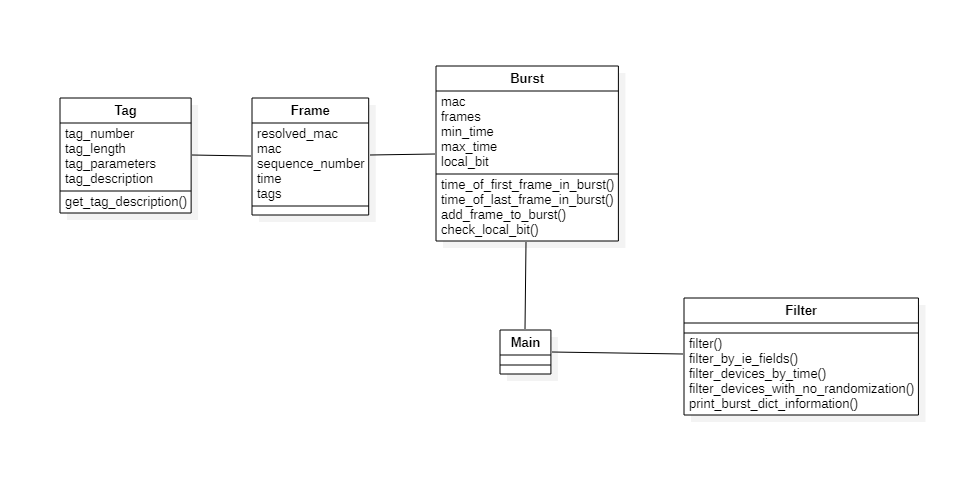
\includegraphics[width=1\linewidth]{Prototype/Klassendiagramm.PNG}
    \caption{Klassendiagramm des Prototyps
	\label{figure:prototypearchitecture}}
\end{figure}

\subsection{Beschreibung der Klassen}
\subsubsection*{Main-Klasse}
Die Main-Klasse ist der Einstiegspunkt in das Programm. 
Darin werden Probe-Requests aus einer angegebenem JSON-Datei ausgelesen,
decodiert und in Frame-Instanzen gespeichert. 
Diese Frame-Instanzen werden dann nach ihrer MAC-Adresse sortiert und 
in Burst-Instanzen gespeichert.
Nachdem die Probe-Requests durch das Preprocessing in Bursts gruppiert wurden,
wird eine Filterklasse instanziert und kann auf die Bursts angewandt werden.

\clearpage 

\subsubsection*{Burst-Klasse}
Ein Burst besteht aus mehreren Probe-Request-Frames mit der gleichen 
MAC-Adresse.
Die Burst Klasse beinhaltet einen bis mehrere Frames in einer Liste, 
welche aufsteigend nach der Ankunftszeit der Frames sortiert ist.
Die Tabelle~\ref{table:burstfields} beschreibt die Klassenvariablen.

\begin{table}[h!]
    \centering
    \begin{tabular}{|l|l|}
        \hline
        \textbf{Variable} & \textbf{Beschreibung} \\
        \hline 
        mac & Die MAC-Adresse der Frames im Burst. \\
        \hline
        frames & Eine Liste mit Frame-Objekten, die im Burst vorkommen. \\
        \hline
        min\_time & Ankunftszeit des ersten Frame im Burst. \\
        \hline
        max\_time & Ankunftszeit des letzten Frame im Burst. \\
        \hline
        local\_bit & Indikator, ob das lokale Bit gesetzt ist. \\
        \hline
    \end{tabular}
    \caption{Klassenvariablen der Burst-Klasse
    \label{table:burstfields}}  
\end{table}

Die Klasse beinhaltet vier Klassenmethoden gemäss der 
Tabelle~\ref{table:burstmethods}.

\begin{table}[h!]
    \centering
    \begin{tabular}{|l|l|}
        \hline
        \textbf{Methode} & \textbf{Beschreibung} \\
        \hline 
        time\_of\_first\_frame\_in\_burst & Evaluiert die Ankunftszeit des ersten \\
        & Frame im Burst. \\
        \hline
        time\_of\_last\_frame\_in\_burst & Evaluiert die Ankunftszeit des letzten \\
        & Frame im Burst. \\
        \hline
        add\_frame\_to\_burst & Fügt ein weiteres Frame zum Burst\\
        & hinzu. \\
        \hline
        check\_local\_bit & Evaluiert anhand der MAC-Adresse, \\
        & ob das local Bit gesetzt ist. \\
        \hline
    \end{tabular}
    \caption{Klassenmethoden der Burst-Klasse
    \label{table:burstmethods}}  
\end{table}

\clearpage 

\subsubsection*{Frame-Klasse}
Die Frame-Klasse beinhaltet jeweils einen einzelnen Probe-Request-Frame, 
welcher in den Messungen aufgezeichnet wurde.
Die Tabelle~\ref{table:framefields} beschreibt die Klassenvariablen. 
Die Frame-Klasse beinhaltet keine Klassenmethoden. 

\begin{table}[h!]
    \centering
    \begin{tabular}{|l|l|}
        \hline
        \textbf{Variable} & \textbf{Beschreibung} \\
        \hline 
        resolved\_mac & Die MAC-Adresse aufgelöst nach Hersteller, falls eine \\
        & Auflösung durch Wireshark vorgenommen wurde. \\
        \hline
        mac & Die MAC-Adresse des Frame. \\
        \hline
        sequence\_number & Die Sequenznummer des Frame. \\
        \hline
        time & Ankunftszeit des Frame. \\
        \hline
        tags & Liste mit Tag-Objekten, welche die \\ 
        & Information-Element-Felder 
        repräsentieren. \\
        \hline
    \end{tabular}
    \caption{Klassenvariablen der Frame-Klasse
    \label{table:framefields}}  
\end{table}

\subsubsection*{Tag-Klasse}
Tags werden verwendet, um die Information-Element-Felder zu repräsentieren.
Die verwendeten Klassenvariablen sind in der Tabelle~\ref{table:tagfields} 
dargestellt.

\begin{table}[h!]
    \centering
    \begin{tabular}{|l|l|}
        \hline
        \textbf{Variable} & \textbf{Beschreibung} \\
        \hline 
        tag\_number & Nummer des IE-Felds gemäss IEEE 802.11 \\
        \hline
        tag\_length & Grösse des Information-Element-Felds \\
        \hline
        tag\_parameters & Liste mit weiteren Informationen im IE-Feld. \\
        \hline
        tag\_description & Bezeichnung des Information-Element-Felds. \\
        \hline
    \end{tabular}
    \caption{Klassenvariablen der Tag-Klasse
    \label{table:tagfields}}  
\end{table}

Die Tag-Klasse beinhaltet die Klassenmethode "get\_tag\_description", 
welche aus einem Dictionary die Bezeichnung der Information-Element-Felder 
ausliest.

\clearpage

\subsubsection*{Filter-Klasse}
In der Filter-Klasse sind die einzelnen Filtermethoden umgesetzt, 
welche für die Klassifikation der Probe-Requests verwendet werden. 
Die Methoden nehmen als Input jeweils einen Dictionary mit Burst-Klassen 
entgegen und geben als Output ebenfalls einen Dictionary mit Burst-Klassen zurück.
Die Eigenschaft, dass der Input und Output der Methoden in identischem Format 
gehalten wird, erlaubt eine beliebige Reihenfolge der Methodenaufrufe.
Die einzelnen Filtermethoden sind in der Tabelle~\ref{table:filtermethods}
beschrieben.

\begin{table}[h!]
    \centering
    \begin{tabular}{|l|l|}
        \hline
        \textbf{Methode} & \textbf{Beschreibung} \\
        \hline 
        filter & Führt alle Filtermethoden \\
        & der Filterklasse aus. \\
        \hline
        filter\_by\_ie\_fields & Klassifiziert Frames anhand der \\
        & Information-Element-Felder. \\
        \hline
        filter\_devices\_by\_time & Klassifiziert Frames nach ihrer\\
        & Ankunftszeit. \\
        \hline
        filter\_devices\_with\_no\_randomization & Erkennt, ob in mehreren Bursts \\
        & die selbe MAC-Adresse verwendet\\ 
        &wurde  und fasst diese in einer\\
        & Liste zusammen. \\
        \hline
        print\_burst\_information & Methode für die Ausgabe der \\
        & Filterresultate. \\
        \hline
    \end{tabular}
    \caption{Klassenmethoden der Filter-Klasse
    \label{table:filtermethods}}  
\end{table}
       
Die Filterung nach Ankunftszeit kann, wie im 
Unterabschnitt~\ref{subsection:timefilter} beschrieben, 
nicht erfolgreich durchgeführt werden. 
Die Methode wurde der Vollständigkeit halber im Prototyp belassen, und kann 
verwendet werden, um aufzuzeigen, dass eine Filterung nach Ankunftszeit 
keine erfolgreiche Klassifikation durchführt.

\clearpage
\section{Prototyp-Verifikation
\label{section:verification}}
Um die Funktionalität des Prototyps zu verifizieren, wurden insgesamt sechs
separate Messungen durchgeführt. Diese Messungen beinhalten - abgesehen von 
einer Messung - alle merhere Mobilgeräte. Die Messparameter und der Verwendungszweck
sind in den nachfolgenden Unterabschnitten beschrieben.

\subsection{Messungen für die Verifikation}
\subsubsection*{Fairphone Gemischt Aktiv/Passiv}
In der 30-Minütigen Messung wurde in einem fünf-Minuten-Intervall zwischen 
aktivem und passivem verhalten auf dem Fairphone 3+ gewechselt.
Mit diesen Messdaten wurde überprüft, ob der Prototyp in der Lage ist, 
Geräte zu erkennen, die während der Probe-Request-Aufzeichnung zwischen Aktiv/Passiv 
wechseln.

Die Prototyp-Verifikation hat gezeigt, dass der Prototyp Geräte, 
die unterschiedliche IE-Felder im aktiven oder passiven Modus verwenden, 
als zwei separate Geräte klassifiziert. Eine Auswertung der verwendeten 
IE-Felder hat gezeigt, dass ausser dem Fairphone 3+ alle Geräte mehrheitlich 
die gleichen IE-Felder im aktiven wie auch im passiven Modus verwenden.

Die Abbildung~\ref{figure:fairphonemixed} zeigt das Resultat des Prototypen 
für die Messung.

\begin{figure}[h!]
	\centering
	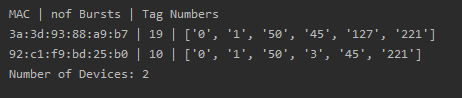
\includegraphics[width=0.75\linewidth]{Prototype/fairphone_gemischt_verifikation.PNG}
    \caption{Ausgabe des Prototyps für die Messung 
	\label{figure:fairphonemixed}}
\end{figure}

\clearpage 


\subsubsection*{Fairphone iPhone Aktiv}
In der 30-Minütigen Messung wurden Probe-Requests des iPhone X und des 
Fairphone 3+ im aktiven Modus aufgezeichnet. 
Mit den Messdaten wurde überprüft, ob der Prototyp zwischen einem 
Android- und einem iOS-Gerät unterscheiden kann.

Der Prototyp konnte in dieser Messung das Fairphone 3+ vom iPhone X unterscheiden,
wie die Abbildung~\ref{figure:fairphoneiphoneactive} zeigt.

\begin{figure}[h!]
	\centering
	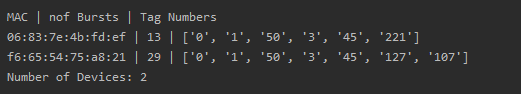
\includegraphics[width=0.75\linewidth]{Prototype/Fairphone_iphone_aktiv_verifikation.PNG}
    \caption{Ausgabe des Prototyp für die Messung 
	\label{figure:fairphoneiphoneactive}}
\end{figure}


\subsubsection*{Fairphone iPhone Passiv}
In der 30-Minütigen Messung wurden Probe-Requests des iPhone X und des 
Fairphone 3+ im passiven Modus aufgezeichnet. 
Mit den Messdaten wurde überprüft, ob der Prototyp zwischen einem 
Android- und einem iOS-Gerät unterscheiden kann.

In der Passivmessung ist nur ein Burst des Fairphone aufgetreten und der 
Prototyp hat diese falsch als Störeinfluss klassifiziert und 
nicht beachtet.
Man kann in der Abbildung~\ref{figure:fairphoneiphonepassiveone} sehen, 
dass nur ein Gerät erkannt wird.

\begin{figure}[h!]
	\centering
	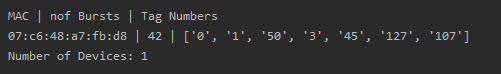
\includegraphics[width=0.75\linewidth]{Prototype/Fairphone_iphone_passiv_2_verifikation.PNG}
    \caption{Ausgabe des Prototyp für die Messung 
	\label{figure:fairphoneiphonepassiveone}}
\end{figure}

Man kann im Prototyp einstellen, wieviele Bursts in einer Liste vorkommen müssen, 
damit die Liste als separates Gerät gespeichert wird.
Man sieht in Abbildung~\ref{figure:fairphoneiphonepassivetwo} das Resultat, wenn ein Burst ausreicht, 
damit die Liste als Gerät akzeptiert wird.

\begin{figure}[h!]
	\centering
	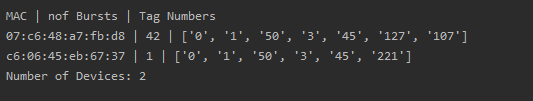
\includegraphics[width=0.75\linewidth]{Prototype/Fairphone_iphone_passiv_1_verifikation.PNG}
    \caption{Ausgabe des Prototyp für die Messung 
	\label{figure:fairphoneiphonepassivetwo}}
\end{figure}

\clearpage 

\subsubsection*{Pixel iPhone S20 Aktiv}
In der 60-Minütigen Messung wurden Probe-Requests des Google Pixel 3, des iPhone X
und des Samsung Galaxy S20+ im aktiven Modus aufgezeichnet.
Mit den Messdaten wurde überprüft, ob der Prototyp zwischen dreien Geräten 
unterscheiden kann.

Der Prototyp kann in der Messung erfolgreich die drei Geräte klassifizieren.
Die Abbildung~\ref{figure:threephonesactive} zeigt die Ausgabe des Prototyps. 

\begin{figure}[h!]
	\centering
	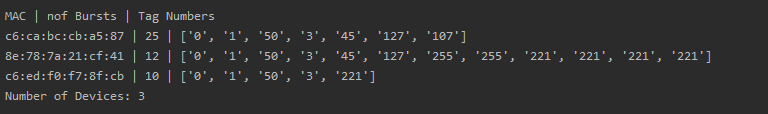
\includegraphics[width=0.75\linewidth]{Prototype/Pixel_iPhone_S20_aktiv_verifikation.PNG}
    \caption{Ausgabe des Prototyp für die Messung 
	\label{figure:threephonesactive}}
\end{figure}


\subsubsection*{Pixel iPhone S20 Passiv}
In der 60-Minütigen Messung wurden Probe-Requests des Google Pixel 3, des iPhone X
und des Samsung Galaxy S20+ im passiven Modus aufgezeichnet.
Mit den Messdaten wurde überprüft, ob der Prototyp zwischen dreien Geräten 
unterscheiden kann.

Auch in der Passivmessung wurden alle drei Geräte korrekt klassifiziert,
wie in der Abbildung~\ref{figure:threephonespassive} ersichtlich.

\begin{figure}[h!]
	\centering
	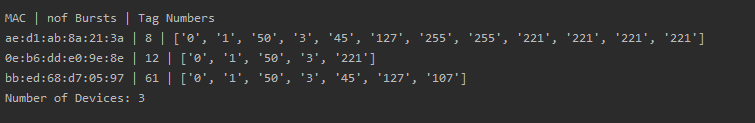
\includegraphics[width=0.75\linewidth]{Prototype/Pixel_iPhone_S20_passiv_verifikation.PNG}
    \caption{Ausgabe des Prototyp für die Messung 
	\label{figure:threephonespassive}}
\end{figure}

\clearpage 

\subsubsection*{Sechs Mobilgeräte Gemischtes Verhalten}
In dieser Messung wurden 20 Minuten lang Probe-Requests von sechs verschiedenen
Mobilgeräten aufgezeichnet. Dabei wechseln die Mobilgeräte zwischen Aktiv/Passiv, 
verbinden sich zwischendurch mit einem WLAN oder werden in den Flugmodus geschaltet.
Die Messung soll in einem kleineren Rahmen das Verhalten von Passagieren in einem 
Zug simulieren und dient der Verifikation des Prototyps mit realistischen Messdaten.

Der Prototyp erkennt acht verschiedene Geräte in der Messung.
Dies kann damit erklärt werden, dass ein Gerät je nachdem, ob es Aktiv oder Passiv ist,
separat erkannt und klassifiziert wird, wie bereits mit der Messung des Fairphone 3+ 
gezeigt. 
In der Abbildung~\ref{figure:allthephones} ist die Ausgabe des Prototyp ersichtlich.

\begin{figure}[h!]
	\centering
	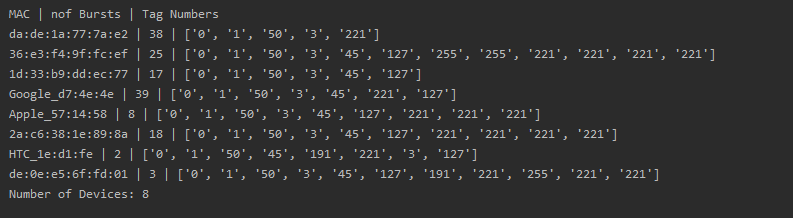
\includegraphics[width=0.85\linewidth]{Prototype/All_the_phones_realistic_verification.PNG}
    \caption{Ausgabe des Prototyp für die Messung 
	\label{figure:allthephones}}
\end{figure}

Weiterhin ist es nicht ausgeschlossen, dass ein Gerät von ausserhalb der Messkammer
aufgezeichnet wurde, da in den Versuchen kein HTC-Gerät verwendet wurde. 

\clearpage




\part{Abschluss}
\section{Weiterführende Arbeiten}
\subsection{Entwicklung einer Zähleinrichtung}
Der in dieser Arbeit entwickelte Prototyp ist darauf ausgelegt, zuvor durchgeführte
Wireshark-Messungen auszuwerten.
Damit Messungen in der Praxis, beispielsweise in einem Zug oder Tram durchgeführt
werden können, muss der Prototyp dahingehend erweitert werden, dass 
Probe-Requests kontinuierlich erfasst und ausgewertet werden können.
Dazu wurden ein Architekturvorschlag erarbeitet, der in einer künftigen 
Arbeit als Anhaltspunkt dienen kann.

\subsubsection*{Architekturvorschlag}
Eine Möglichkeit, wie die Architektur einer Zähleinrichtung aufgebaut werden könnte,
wird in der Abbildung~\ref{figure:architectureproposal} dargestellt.

\begin{figure}[h!]
    \centering
    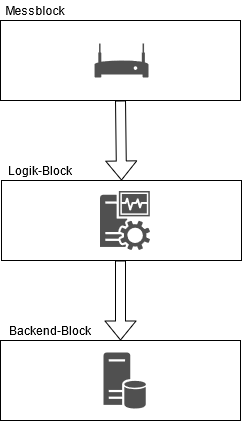
\includegraphics[width=0.5\linewidth]{architectureproposal.png}
    \caption{Architekturvorschlag für eine Zähleinrichtung}
    \label{figure:architectureproposal}
\end{figure}

\clearpage

Im Messblock befinden sich ein oder mehrere Access-Points oder Messantennen, 
welche ankommende Probe-Requests erfassen und an den Logik-Block weiterleiten.
Der Logik-Block ist für die Sortierung und Filterung der ankommenden Probe-Requests
verantwortlich. Die Resultate werden dann an einen Backend-Block weitergeleitet,
welcher für eine Persistierung der Ergebnisse und allfällige Auswertungen 
verantwortlich ist. Falls die Architektur mit einem IOT-Ansatz umgesetzt wird, 
kann durch eine Vorfilterung im Messblock die benötigte Bandbreite für die 
Übertragung reduziert werden. Weiterhin muss in solch einem Ansatz evaluiert 
werden, ob sich der Logik-Block vor Ort in Form eines Gateway befindet oder 
auf dem Server realisiert wird.

Ein weiterer möglicher Ansatz für eine Zähleinrichtung ist die Verwendung 
von Raspberry Pi als abgeschlossenes Zählsystem. Es ist möglich mit einem -
oder mehreren - Raspberry Pi mit WLAN-Dongles ein Messsystem zu entwickeln, 
welches Probe-Requests erfassen und filtern kann. Eine Möglichkeit ist 
die Verwendung eines der Python-Module 
"Pyshark" \footnote{Dokumentation: \url{https://kiminewt.github.io/pyshark/}}
oder "Scapy" \footnote{Dokumentation: \url{https://scapy.readthedocs.io/en/latest/introduction.html}} 
welche beide in der lage sind, WLAN-Daten zu erfassen und zu filtern.


\subsection{Erweiterung der Filterung - Algorithmen}
Eine zusätzliche Möglichkeit, den Prototypen zu verbessern, ist, die 
Algorithmen zu erweitern. Die Filterregeln können beispielsweise durch 
Machine-Learning-Algorithmen dahingehend angepasst werden, dass der 
Prototyp selbständig und kontinuierlich die Klassifikation der Probe-Requests 
ver-bessert.

Dazu müssten weitere Messungen durchgeführt werden, in denen mehrere Geräte 
zur selben Zeit mit verschiedenen Einstellungen in Betrieb sind. 
Dieses Vorgehen würde einen Supervised-Learning-Ansatz ermöglichen.
Alternativ kann auch mit Datensets aus der Praxis gearbeitet werden, 
welche mit einem Unsupervised-Learning-Ansatz einen Algorithmus trainieren.

Werden mehrere Messantennen für die Aufzeichung von Probe-Requests verwendet,
können zusätzliche Informationen bei den Messdaten hinzukommen. 
Beispielsweise ist die Information, welche Antenne den Probe-Request aufgezeichnet
hat, in einer Filterung verwendbar. Allerdings muss darauf geachtet werden, 
dass Frames von einem Gerät, die von mehreren Antennen gleichzeitig aufgezeichnet 
werden, nicht als separate Frames interpretiert werden.

\subsection{Erweiterung der Filterung - Messungen}
In dieser Arbeit wurden zwölf verschiedene Geräte mit insgesamt dreizehn 
Betriebssystemversionen getestet. Die neuste Android-Version 11 konnte nur
auf einem Gerät getestet werden, da die gerätespezifische Android-11-Version 
auf keinem der getesteten Geräte zur Verfügung stand. Weitere Messungen auf 
diesen Gerätetypen mit der Android Version 11 können neue Erkenntnisse 
generieren, mit denen der Prototyp weiter verbessert werden kann oder 
die eine Unterscheidung von Geräten komplett unmöglich machen.

Weiterhin können andere moderne Geräte getestet werden, um den Katalog von 
Geräteverhalten zu erweitern und den Prototypen zu verbessern.

\subsection{Erweiterung der Aufzeichnungsmethoden}
Im Rahmen dieser Arbeit wurde das Verhalten der Mobilgeräte beim Aus-senden 
von Probe-Requests erfasst. Künftige Arbeiten könnten neben Probe-Requests auch 
weitere Informationen von Mobilgeräten aufzeichnen. Eine mögliche Informationsquelle
wären Bluetooth-Signale oder andere Frame-Typen aus der Sicherungsschicht.

Zudem gibt es im Forschungsfeld der Indoor-Lokalisierung den Ansatz, die 
Position eines Mobilgeräts anhand der Signalstärke zu triangulieren.

\clearpage
\section{Abschliessendes Urteil}
In dieser Arbeit wurden Messungen durchgeführt, um das Probing-Verhal-ten von 
modernen Mobilgeräten und aktuellen Betriebssystemen zu ermitteln.
Anhand der Erkenntnisse aus diesen Messungen wurde ein Prototyp entwickelt, 
welcher aufgrund von aufgezeichneten Probe-Requests die Anzahl Mobilgeräte 
im Empfangsbereich berechnet. Dazu wurden Filterregeln in einem hierarchischen 
Filtervorgang implementiert. Der Prototyp wurde an dafür aufgezeichneten Messungen
mit mehreren paralell laufenden Ge-räten validiert und konnte die Anzahl Geräte
zum Teil korrekt ausgeben. Eine Validierung mit Messdaten aus der Praxis konnte 
nicht durchgeführt werden, da kein Datenset zur Verfügung stand, welches mehrere
Mobilgeräte beinhaltet aber auch die Gesamtzahl von Mobilgeräten erfasst hat.

Die in den Messungen aufgezeichneten Probe-Requests beinhalten zu wenige 
voneinander unterscheidbare Parameter, dass damit Geräte mit einem Fingerabdruck
versehen werden können. 
Fingerprinting von Mobilgeräten anhand von Probe-Requests wird mit neu 
erscheinenden Betriebssystemversionen immer schwieriger.
Es ist schon nicht mehr möglich iPhones mit iOS-14 voneinander zu unterscheiden 
und neuere Android-Versionen wird die randomisierung von Probe-Requests eher 
verbessern, als sie zu verschlechtern. 

Somit sind Probe-Requests künftig nicht mehr für Fingerprinting nutzbar.
Um bestehende Verfahren weiterhin nutzen zu können, müssen diese weiterentwickelt 
oder durch andere Verfahren ergänzt werden.

% Project documentation
% ====================
\part{Projektmanagement}
\section{Changelog}
\begin{table}[H]
	\centering
	\begin{tabularx}{\linewidth}{l l X l}
		\toprule 
		\textbf{Date} & \textbf{Version} & \textbf{Changes} & \textbf{Autor} \\
		\midrule
		16.09.2020 & 0.1 & Erstfassung & Mike Schmid \\
		22.09.2020 & 0.2 & Korrekturen & Mike Schmid \\
		29.09.2020 & 0.3 & Anpassungen Risikoanalyse & Mike Schmid \\
		08.11.2020 & 0.4 & Anpassung Iterationen und Meilensteine & Mike Schmid \\
		15.12.2020 & 0.5 & Korrektur Abgabedatum vom 08.11 auf den 15.01.2021 & Mike Schmid \\
		\multirow{2}{*}{03.01.2021} & \multirow{2}{*}{1.0} & \multirow{2}{=}{Finalisieren der Projektdokumentation} & Janik Schlatter \& \\
		& & & Mike Schmid\\
		\bottomrule 
	\end{tabularx} 
	\caption{Changelog Projektmanagement} 
\end{table}

\clearpage

\section{Einführung} 

\subsection*{Zweck}
Dieser Teil der Dokumentation beschreibt die Projektplanung und bietet 
eine Übersicht über den Verlauf der Bachelorarbeit "Mobile Fingerprinting". 
Im Detail wird auf die Planung, Organisation und den Projektaufbau und -ablauf 
eingegangen.

\subsection*{Gültigkeit}
Der Gültigkeitsbereich ist auf die Dauer der Durchführung der Bachelorarbeit 
"Mobile Fingerprinting" im Herbstsemester 2020 an der Fachhochschule OST 
beschränkt.

\subsection*{Sprache}
Die allgemeine Projektsprache (Dokumentation, Protokolle, etc.) wird in 
deutscher Schriftsprache verfasst. 
Der Code, das GitHub-Repository und die Versionskontrolle wird in 
englischer Sprache geschrieben.

\subsection*{Referenzen}
Alle Dokumente werden auf dem GitHub-Repository 
\footnote{
	\hyperref[Repository]{
		https://github.com/EkoGuandor229/BA-MobileFingerprinting
	}
} abgelegt und verwaltet.


\subsection*{Vorarbeit}
Im Vorjahr wurde eine Studienarbeit mit dem Namen "Passenger Tracking" 
durchgeführt, die versucht hat, mittels Machine Learning ein Programm 
zu entwickeln, welches Passagiere im öffentlichen Verkehr anhand der 
von den Mobilgeräten ausgesendeten Probe-Requests erkennen kann. 
Dazu wurden den Studierenden 170 Millionen gesammelte WLAN-Daten vom 
Industriepartner für das Training des Algorithmus zur Verfügung gestellt. 
Der Prototyp konnte die Anzahl Geräte in einem Bus mittels eines Clustering 
Algorithmus mit durchschnittlich 94\% Genauigkeit ermitteln.

Diese Bachelorarbeit soll sich im Gegensatz zur Vorarbeit direkt 
mit dem Verhalten der Mobilgeräte auseinandersetzen. 
Wie wird die MAC-Address-Randomisierung von verschiedenen 
Herstellern mit unterschiedlichen Betriebssystemversionen durchgeführt 
und wie kann man die Unterschiede dafür nutzen, ein Gerät eindeutig zu 
identifizieren und zu verfolgen?

\clearpage

\section{Projektübersicht
\label{Projektübersicht}} 
Auszug aus der Aufgabenstellung:\newline
"Smartphones senden regelmässig WLAN-Probe-Requests, 
um Access Points zu finden. 
In der Vergangenheit konnte durch das Auslesen der MAC-Adresse aus 
diesen Requests ein Gerät über längere Zeit verfolgt werden.

Seit einigen Jahren wird diese Verfolgung durch die Verwendung von
anonymi-sierten MAC-Adressen erschwert. 
Weitere Datenfelder in diesen Requests können für das Tracken aber
weiterhin von Nutzen sein.

In einer früheren Arbeit wurde anhand bestehender Daten eines 
Industriepartners ein Top-Down-Ansatz mittels Machine Learning erarbeitet,
der aber nicht zu genügend genauen Resultaten führte."

\subsection*{Zweck und Ziel}
Das Verschleiern von MAC-Adressen durch Randomisierung ist seit einigen 
Jahren eine gängige Praxis, um die Verfolgung von Benutzern durch 
Organisationen oder Einzelpersonen zu verhindern. Dabei spielt es keine 
Rolle, ob die Verfolgung für statistische Zwecke, für personalisierte 
Werbung oder mit böswilligen Absichten geschieht.

Diese Arbeit befasst sich damit, wie diese Verschleierung von einzelnen 
Anbietern von Mobilgeräten durchgeführt wird und ob sich die Umsetzung
in unterschiedlichen Betriebssystemversionen unterscheidet. 
Durch Experimente soll herausgefunden werden, wie die Verschleierung 
in modernen Geräten in verschiedenen Versionen der Betriebssysteme 
umgesetzt wird. Weiterhin soll ein Prototyp entwickelt werden, 
der die gewonnenen Erkenntnisse umsetzt und die Verfolgung eines 
Gerätes über mehrere WLAN-Access-Points ermöglicht. Die für das 
Training und die Verifizierung des Prototyps benötigten Daten sollen 
in den Experimenten erfasst und aufbereitet werden.

\clearpage

\subsection*{Lieferumfang}
\begin{itemize}
	\item Auswertung, wie die Randomisierung bei MAC-Adressen von
	verschiedenen Anbietern, Mobilgeräten und Betriebssystemen umgesetzt
	wird und welche weiteren Eigenschaften/Attribute von Probe-Requests 
	sonst noch zur Erkennung verwendet werden können.
	\item Proof-of-Concept Prototyp, der die Verfolgung eines 
	zuvor kategorisierten Mobilgerätes (potentiell über mehrere 
	WLAN-Access-Points)	ermöglicht, falls möglich.
	\item Source-Code des Prototyps
	\item Protokolle, Dokumentation und gewonnene Daten der Experimente
	\item Sitzungsprotokolle
	\item Bericht der Bachelorarbeit gem. den Vorgaben der Hochschule 
	und des Projektbetreuers
	\item Abstract der Arbeit für das Online-Tool der Hochschule
	\item Plakat mit den wichtigsten Eckpunkten für die 
	Bachelorarbeitspräsentation
	\item Eigenständigkeitserklärung
	\item Einverständniserklärung für die Publikation
	\item Vereinbarung über Urheber- und Nutzungsrechte
\end{itemize} 

\subsection*{Annahmen und Einschränkungen}
Für die Bachelorarbeit sind 12 ECTS vorgesehen. 
Pro Person fällt somit ein Arbeitsaufwand von 360 Stunden, 
für die Arbeit gesamthaft 720 Stunden an.
Die Bachelorarbeit muss bis zum 15.01.2021 abgegeben werden.

\clearpage

\section{Projektorganisation 
\label{Projektorganisation}}

\subsection*{Projektmitglieder}
\begin{table}[H]
	\centering
	\begin{tabularx}{\linewidth}{X X}
		Mike Schmid & Janik Schlatter \\
		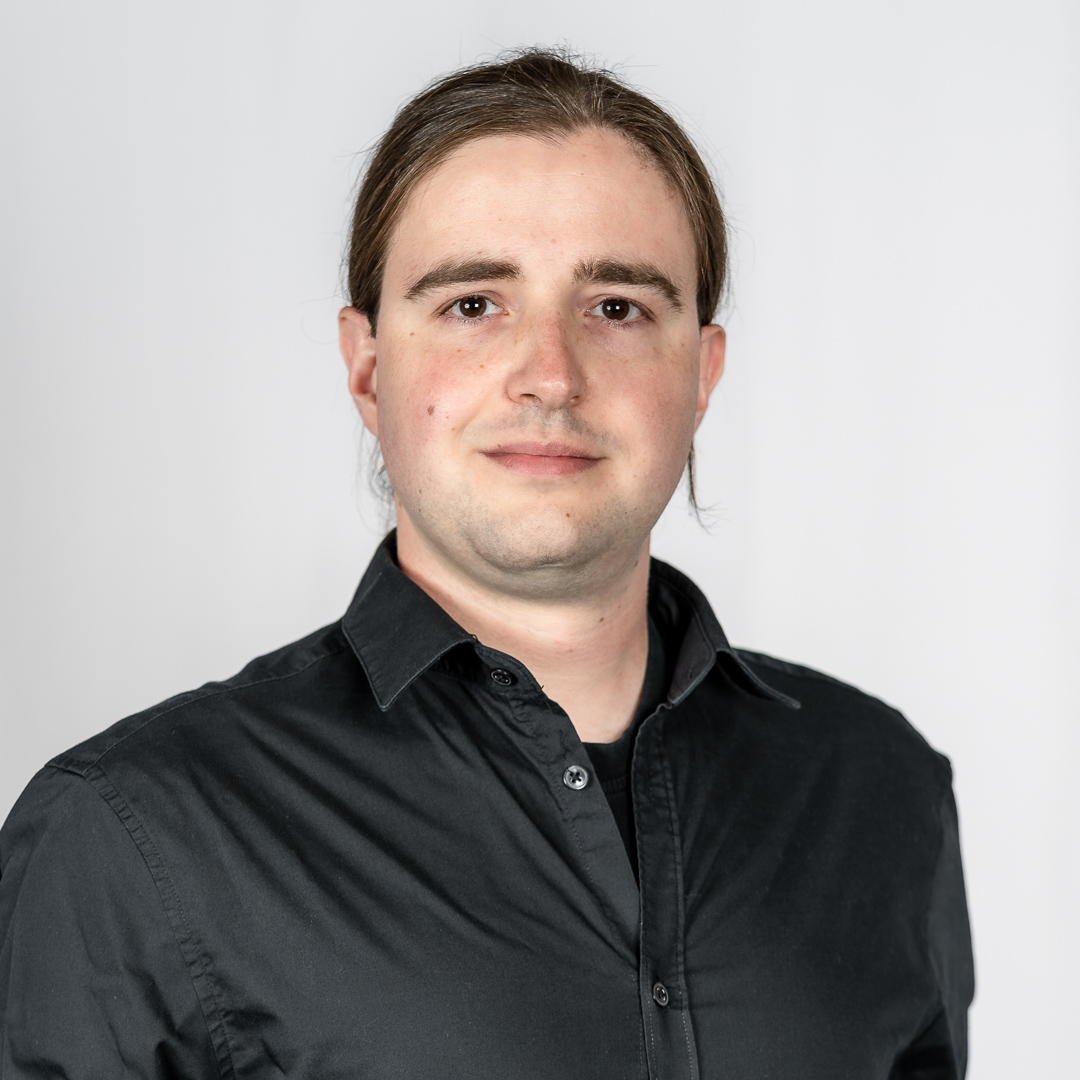
\includegraphics[width=0.75\linewidth]{Portrait_Schmid_Mike-2.jpg}
		&
		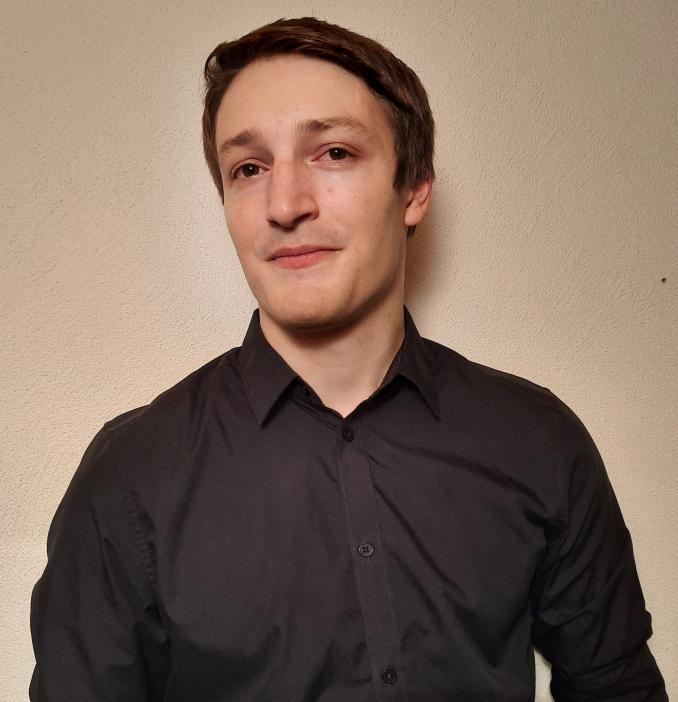
\includegraphics[width=0.73\linewidth]{Portrait_Janik.png}
	\end{tabularx} 
\end{table}

\subsection*{Externe Schnittstellen}
\begin{table}[H]
	\centering
	\begin{tabularx}{\linewidth}{| X | X | X |}
		\hline
		Prof. Beat Stettler & Martin Willi & Claudio Fuchs \\
		Betreuer & Experte & Gegenleser\\
		\hline
	\end{tabularx} 
\end{table}

\clearpage

\section{Management 
\label{Management}} 

\subsection*{Eckdaten}
Die Bachelorarbeit startet am 14.09.2020 und endet am 15.01.2021. 
In diesem Zeitraum werden die 360 Stunden Arbeit der einzelnen 
Projektmitglieder erbracht.
Zu Beginn der Arbeit wurde davon ausgegangen, dass die Arbeit in der 
zweiten Januarwoche am 08.01.2021 abgegeben werden muss. 
Die Arbeit wurde auf dieses Abgabedatum hin geplant und durchgeführt.
Die zusätzliche Woche wird als Reservezeit für allfällige Nachbesserungen 
betrachtet.

Gesamthaft stehen in diesem Zeitraum - bis am 08.01.2021 - 17 Wochen zur Verfügung, 
was in einem Wochendurchschnitt von 21.18 Stunden pro Person entspricht. 
Um die Planung zu vereinfachen, wurde die zu leistende Zeit auf 21h/Person 
und Woche festgelegt. 
Die Übrigen drei Stunden werden in der Abschlussphase verwendet, 
um die Dokumentation fertigzustellen. 

\begin{table}[H]
	\centering
	\begin{tabularx}{\linewidth}{X l}
		\toprule 
		Projektdauer & 17 Wochen  \\
		Anzahl Projektmitglieder & 2 \\
		Arbeitszeit für Projekt pro Woche und Mitglied & 21 Stunden \\
		Total Stunden pro Mitglied & 360 Stunden \\
		Arbeitsstunden Total & 720 Stunden \\
		Projektstart & 14.09.2020 \\
		Projektende (geplant) & 08.01.2021 \\
		\bottomrule 
	\end{tabularx} 
\end{table}

Die folgenden Absenzen sind beim Projektbeginn bekannt und eingeplant:
\begin{table}[H]
	\centering
	\begin{tabularx}{\linewidth}{X l l}
		\toprule 
		\textbf{Mitglied} & \textbf{Von} & \textbf{Bis} \\
		\midrule
		Janik Schlatter & 22.10.2020 & 30.10.2020 \\
		Beide & 24.12.2020 & 27.12.2020 \\
		\bottomrule 
	\end{tabularx}  
\end{table}
Jedes Projektmitglied ist selbst dafür verantwortlich, 
die Abwesenheiten entsprechend zu kompensieren.

\clearpage

\subsection*{Zeitliche Planung}
Die 17 Wochen des Projekts werden in vier Phasen unterteilt: 
\begin{itemize}
	\item Initialisierung
	\item Recherche
	\item Experimente, Implementation \& Evaluation
	\item Abschluss
\end{itemize}
In der Abbildung~\ref{figure:Projektphasen} sind die einzelnen 
Phasen ersichtlich. 
Da in der dritten Phase die Implementation davon abhängt, 
dass durch die Experimente statistisch relevante Erkenntnisse gewonnen werden, 
welche für einen Prototypen genutzt werden können, 
vereinheitlicht die dritte Phase die Experimente, 
Evaluation und das Prototyping. 

\begin{figure}[h!]
	\centering
	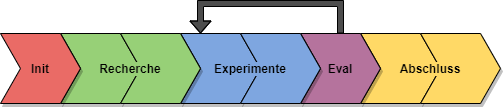
\includegraphics[width=1\linewidth]{ProjektPhasen.png}
	\caption{Projektphasen
	\label{figure:Projektphasen}}
\end{figure}
	
\subsection*{Iterationen}
Eine Iteration beträgt in der zweiten Phase zwei
und in der dritten Phase drei Wochen. 
Jeweils im nächsten Meeting nach einer Iteration werden die gewonnenen 
Erkenntnisse und das weitere Vorgehen besprochen. 
In der Tabelle~\ref{table:Projektiterationen} sind die einzelnen 
Iterationen und deren Tätigkeiten beschrieben.

\begin{landscape}
	\begin{table}[H]
		\centering
		\begin{tabularx}{\linewidth}{l X l l}
			\toprule 
			\textbf{Iteration} & \textbf{Inhalt} & \textbf{Start} & \textbf{Ende} \\
			\midrule
			Initialisierung & Projektstart und Kick-Off Meeting & 14.09.2020 & 20.09.2020 \\
			\midrule
			Research & 
			Wissensaufbau, Dokumentenstudium, Paperstudium und vorbereiten erstes Experiment &
			21.09.2020 &
			04.10.2020 \\
			\midrule
			Experiment 1 & Planen, durchführen und auswerten erstes Experiment & 05.10.2020 & 25.10.2020 \\
			Experiment 2 & Planen, durchführen und auswerten zweites Experiment & 26.10.2020 & 29.11.2020 \\
			Prototype 1 & Implementation erster Prototyp für Klassifizierung eines Mobilgeräts & 30.11.2020 & 13.12.2020 \\
			Experiment/Prototype & Iterativ weitere Experimente oder Weiterentwicklung Prototyp & 14.12.2020 & 27.12.2020 \\
			\midrule
			Abschluss & Fertigstellen Dokumentation, Aufbereiten der Ergebnisse für Abgabe & 28.12.2020 & 08.01.2021 \\
			\bottomrule 
		\end{tabularx} 
		\caption{Projektiterationen
		\label{table:Projektiterationen}} 
	\end{table}
\end{landscape}

\clearpage

\subsection*{Meilensteine}
In der Bachelorarbeit wurden Meilensteine gemäss der 
Tabelle~\ref{table:Meilensteine} festgelegt.
\begin{table}[H]
	\centering
	\begin{tabularx}{\linewidth}{l X l l}
		\toprule 
		\textbf{Meilenstein} & \textbf{Beschreibung} & \textbf{Termin} & \textbf{Aufwand} \\
		\midrule
		M1 & Projektplan & 20.09.2020 & 42h (1 Woche) \\
		M2 & Recherche & 04.10.2020 & 84h (2 Wochen) \\
		M3 & Experimente 1 \& 2 & 29.11.2020 & 336h (8 Wochen) \\
		M4 & Prototyp 1 & 29.11.2020 & 84h (2 Wochen) \\
		M5 & Experiment 3 \& Prototyp 2 & 27.12.2020 & 84h (2 Wochen) \\
		M6 & Schlussabgabe & 08.01.2021 & 84h (2 Wochen) \\
		\bottomrule 
	\end{tabularx} 
	\caption{Meilensteine
	\label{table:Meilensteine}} 
\end{table}

\subsection*{Meetings und Informationsfluss}
Die Projektmitglieder haben drei Tage - Dienstag, Mittwoch und Donnerstag -
an denen sie jeweils gemeinsam an der Bachelorarbeit arbeiten. 
An jedem Tag stehen mindestens sechs Lektionen für die Bearbeitung der 
anstehenden Arbeiten zur Verfügung.

Besprechungen zwischen den Projektteilnehmern und dem Betreuer finden
einmal alle ein bis zwei Wochen statt, um sich über den Stand der Arbeit
und gewonnene Erkenntnisse auszutauschen. 
Meetings können vor Ort an der Hochschule in einem dafür geeigneten Raum 
oder über Microsoft Teams durchgeführt werden.

\fbox{
	\begin{minipage}{\linewidth}
	Die in den Sitzungen besprochenen Pendenzen und Entscheidungen 
	können aus den Sitzungsprotokollen entnommen werden die sich im 
	Anhang~\ref{meetings} befinden.
	\end{minipage}
}

\clearpage

\section{Risikomanagement
\label{Risikomanagement}}
Mögliche Risiken wurden während der Bachelorarbeit fortlaufend evaluiert 
und angepasst, um auf unvorhergesehene Ereignisse möglichst verhältnismässig 
reagieren zu können.

\subsection*{Risiken}
Eine Risikoanalyse mit gewichtetem Schaden und Informationen, 
wie mit diesen Risiken umgegangen wird, 
ist im Dokument «TechnischeRisiken.xlsx» zu finden. 
Die Abbildung~\ref{figure:Risikomatrix} zeigt die Risikomatrix zum Beginn
der Bachelorarbeit am 14.09.2020.

\begin{figure}[h!]
	\centering
	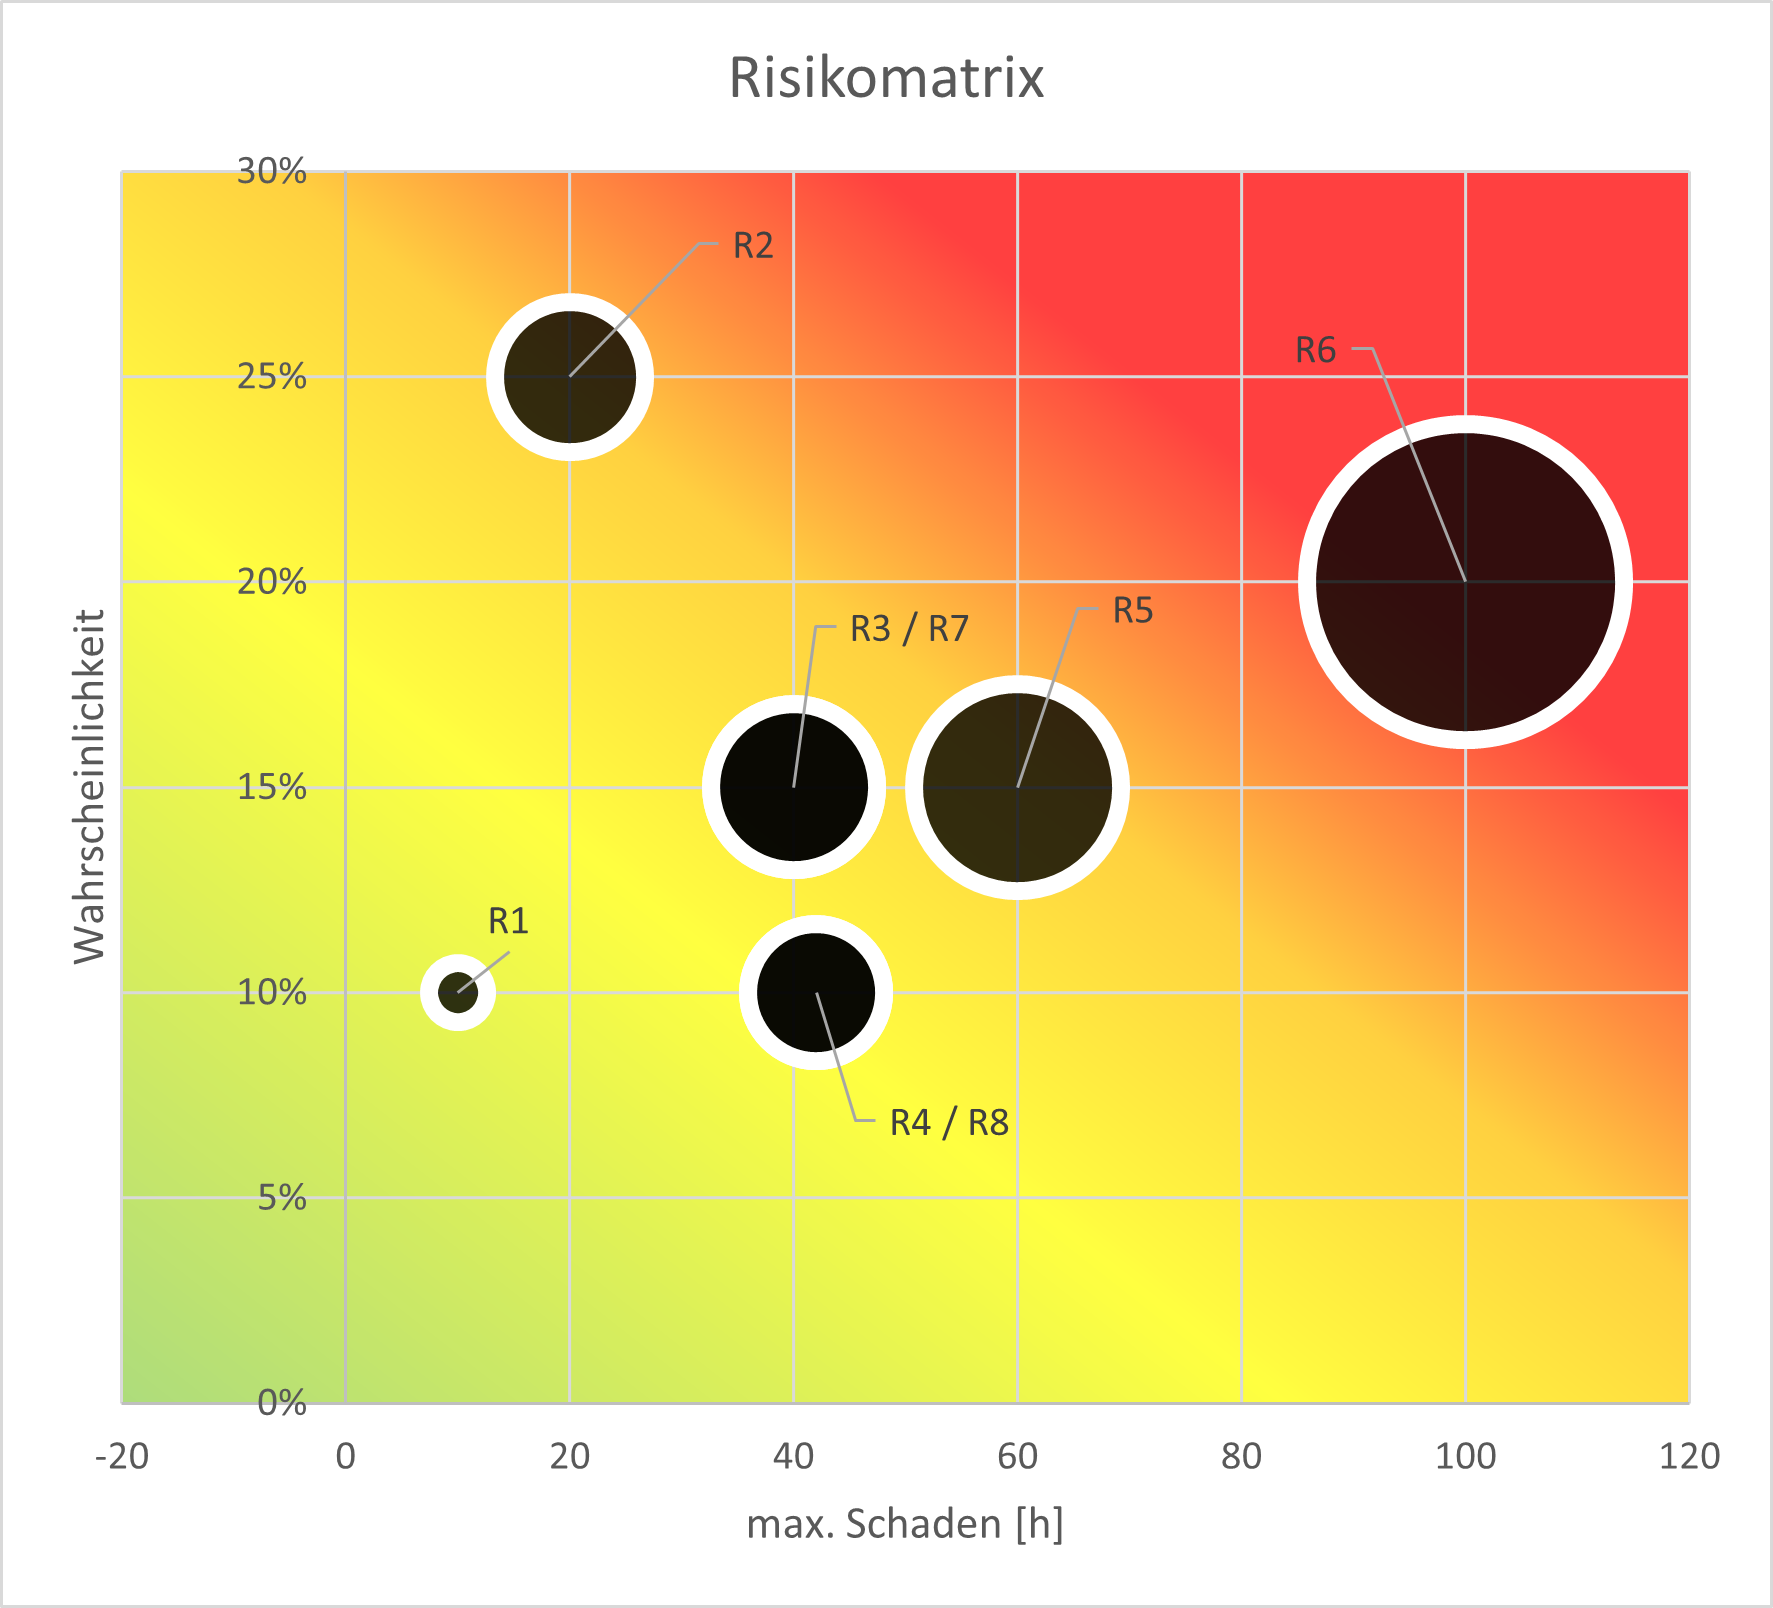
\includegraphics[width=1\linewidth]{RisikoMatrix.png}
	\caption{Risikomatrix, die Grösse der Blasen entspricht dem gewichteten Schaden
	\label{figure:Risikomatrix}}
\end{figure}

\begin{table}[H]
	\centering
	\begin{tabularx}{\linewidth}{| l | X | l | X |}
		\hline
		R1 & Testgeräte & R5 & Format Versuchsdaten \\
		\hline
		R2 & Testvorbereitung & R6 & Gerätemerkmale \\
		\hline
		R3 & Testdurchführung & R7 & Geräteverhalten \\
		\hline
		R4 & Testauswertung & R8 & Hardwareverhalten \\		
		\hline 
	\end{tabularx} 
	\caption{Risiken der Risikomatrix
	\label{table:RisikenMatrix}} 
\end{table}

\clearpage 

\subsection*{Risikoentwicklung und Risikoüberwachung}
Nachfolgend sind in den Tabellen~\ref{table:AenderungRisikoAnalyse}
die Änderungen der Risiken im Verlauf der Bachelorarbeit dokumentiert.

\begin{table}[h!]
	\centering
	\begin{tabularx}{\linewidth}{l l X}
		\toprule 
		\textbf{Risiko} & \textbf{Änderung} & \textbf{Begründung} \\
		\midrule
		R6 Gerätemerkmale & Neues Risiko & Hinzufügen Hardwarerisiken \\
		\midrule
		R7 Geräteverhalten & Neues Risiko & Hinzufügen Hardwarerisiken \\
		\midrule 
		R8 Geräteverhalten & Neues Risiko & Hinzufügen Hardwarerisiken \\ 
		\midrule
		\multirow{2}{*}{R1 Testgeräte} & Schaden: 10h $\rightarrow$ 5h & \multirow{2}{=}{Eingetretenes Risiko} \\
		& Wahrscheinlichkeit: 10\% $\rightarrow$ 5\% & \\
		\midrule
		\multirow{4}{*}{R2 Testvorbereitung} &  &  \multirow{4}{=}{Vorbeugung durch Absprache mit Betreuer} \\
		& Schaden 20h $\rightarrow$ 10h & \\
		& Wahrscheinlichkeit: 25\% $\rightarrow$ 5\% & \\
		& & \\
		\midrule 
		\multirow{2}{*}{R3 Testdurchführung} & Schaden: 40h $\rightarrow$ 30h & \multirow{2}{=}{Eingetretenes Risiko} \\
		& Wahrscheinlichkeit: 15\% $\rightarrow$ 10\% & \\
		\midrule
		R4 Testauswertung & Wahrscheinlichkeit: 10\% $\rightarrow$ 5\% & Vorbeugung \\
		\midrule 
		R5 Format  & \multirow{2}{*}{Wahrscheinlichkeit: 15\% $\rightarrow$ 5\%} & \multirow{2}{*}{Vorbeugung} \\
		Versuchsdaten& & \\
		\midrule  
		R6 Gerätemerkmale & Schaden: 100h $\rightarrow$ 80h & Eingetretenes Risiko \\
		\midrule 
		R7 Geräteverhalten & Schaden: 40h $\rightarrow$ 30h & Eingetretenes Risiko \\
		\bottomrule 
	\end{tabularx} 
	\caption{Änderungen der Risikoanalyse
	\label{table:AenderungRisikoAnalyse}} 
\end{table}

\clearpage 

\subsection*{Eingetretene Risiken}
In der Aufzählung~\ref{figure:EingetreteneRisiken} sind die eingetretenen 
Risiken aufgeführt. 
Risiken aus der Analyse, die nicht in der Aufzählung vorkommen, 
sind im Projektverlauf nicht eingetreten oder konnten durch vorbeugende 
Massnahmen verhindert werden.

\begin{figure}[h!]
	\begin{itemize}
	\item R1 - Testgeräte. Die vorhandene Hardware konnte nicht zur 
	Aufzeichnung der Probe-Requests verwendet werden. Es wurde 
	Frühzeitig ein Ersatzlaptop organisiert. Zeitaufwand: ca. 2 Stunden 
	\item R3 - Testdurchführung. Es mussten zwei zusätzliche Messungen 
	durchgeführt werden, da der ursprüngliche Testplan die benötigten 
	Daten nicht abdeckte. Zeitaufwand: ca. 4 Stunden
	\item R6 - Gerätemerkmale. Die iOS-Geräte liefern zu wenige 
	eindeutige Merkmale, als dass damit ein Fingerprinting durchgeführt
	werden könnte. Es wird in der Dokumentation darauf eingegangen, 
	sonst aber keine Massnahmen ergriffen.
	\item R7 - Geräteverhalten. Die Samsung Galaxy S8 verhalten sich im 
	Timing alle unterschiedlich. Die iPhone X haben unterschiede im Verhalten.
	In der Analyse wurde auf die Unterschiede eingegangen. Kein Zeitverlust.
	\end{itemize}
	\caption{Eingetretene Risiken
	\label{figure:EingetreteneRisiken}}
\end{figure}

\clearpage

\section{Arbeitspakete}
Die Arbeitspakete in der Bachelorarbeit werden mittels eines Excel-Dokuments 
verwaltet. Zu Beginn eines Meilensteins werden, wo sinnvoll, Arbeitspakete
erfasst, deren Zeitaufwand geschätzt und zugeteilt. 

Ein Arbeitspaket beinhaltet:
\begin{itemize}
	\item Titel
	\item Beschreibung
	\item Sub-Tasks
	\item Definition of Done 
	\item Geschätzter Aufwand
	\item Tatsächlich benötigter Aufwand
\end{itemize}

\subsection*{Auswertung der Arbeitspakete}

\subsubsection*{Phase 1: Initialisierung}
\begin{figure}[h!]
	\centering
	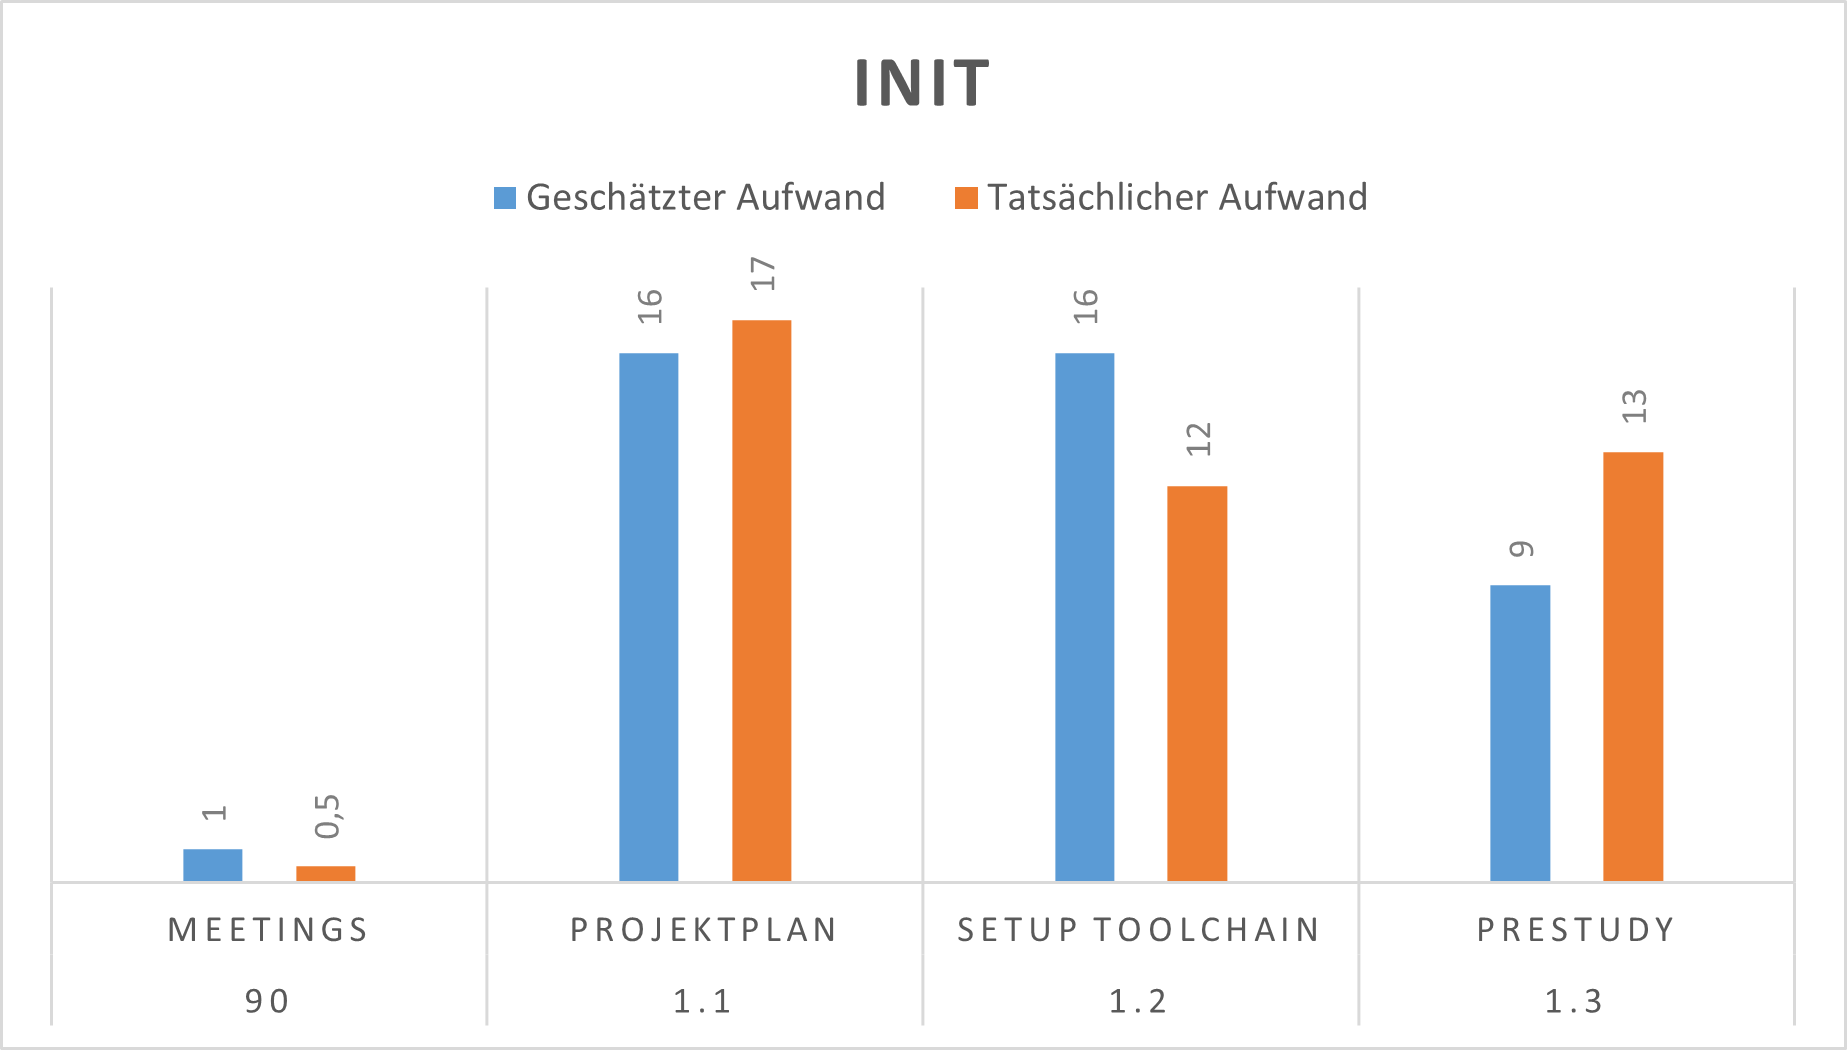
\includegraphics[width=1\linewidth]{Projectmanagement/Init_Auswertung.png}
	\caption{Auswertung der Arbeitspakete in der Initialisierungsphase
	\label{figure:initevaluation}}
\end{figure}

Geplanter Aufwand: $42$ Stunden. \\
Tatsächlicher Aufwand: $42.5$ Stunden.

\clearpage 


\subsubsection*{Phase 2: Recherche}
\begin{figure}[h!]
	\centering
	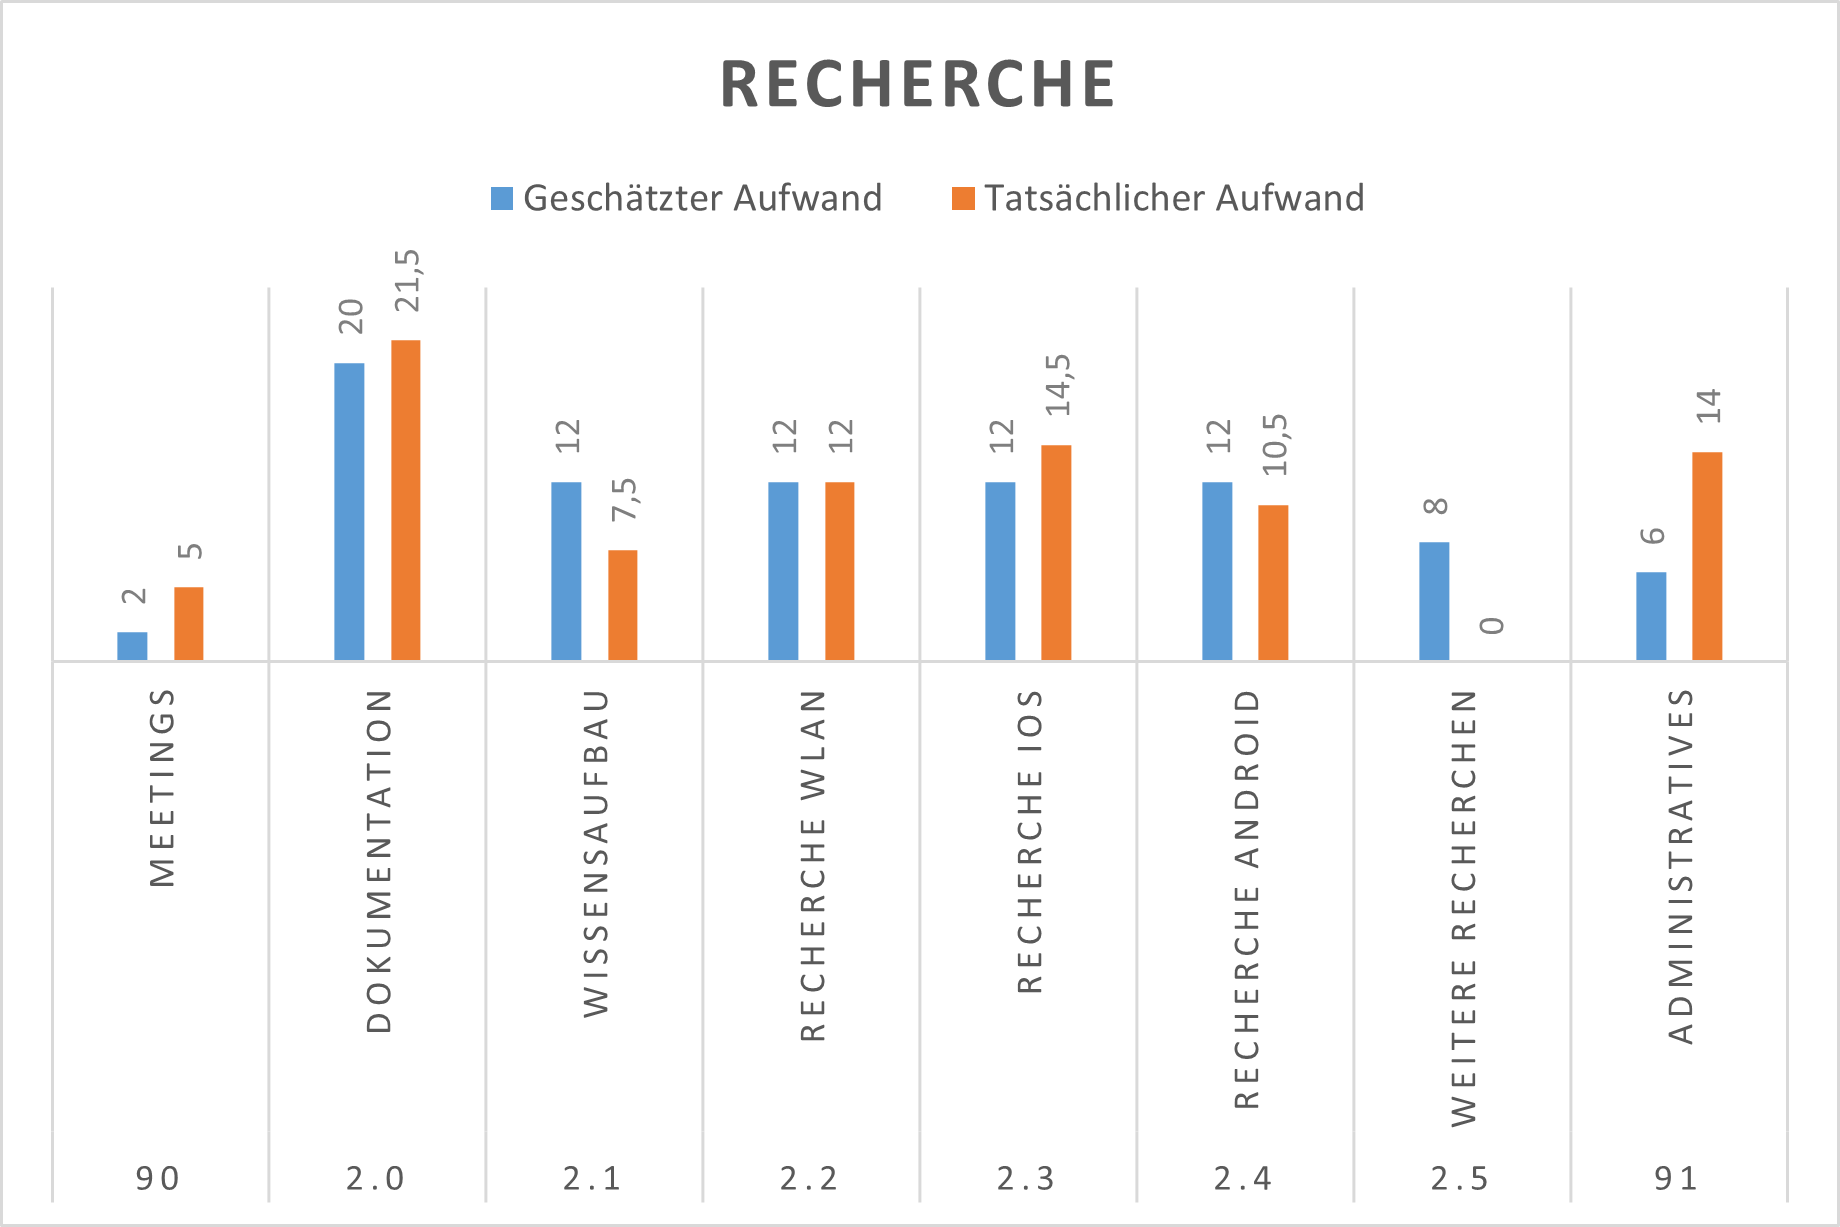
\includegraphics[width=1\linewidth]{Projectmanagement/Recherche_Auswertung.png}
	\caption{Auswertung der Arbeitspakete in der Recherchephase
	\label{figure:researchevaluation}}
\end{figure}

Geplanter Aufwand: $84$ Stunden. \\
Tatsächlicher Aufwand: $85$ Stunden.

Die weiteren Recherchen wurden als Reserve eingeplant, falls sich 
die Projektteilnehmer für die dritte Phase noch zusätzlich in eine Technologie
einarbeiten müssten. 

Vor allem der administrative Aufwand wurde unterschätzt. 
Die Beschaffung der benötigten Mobilgeräte hat mehr Zeit beansprucht, als 
ursprünglich angenommen.  

\clearpage

\subsubsection*{Phase 3: Experimente, Evaluierung und Prototyp}
\begin{figure}[h!]
	\centering
	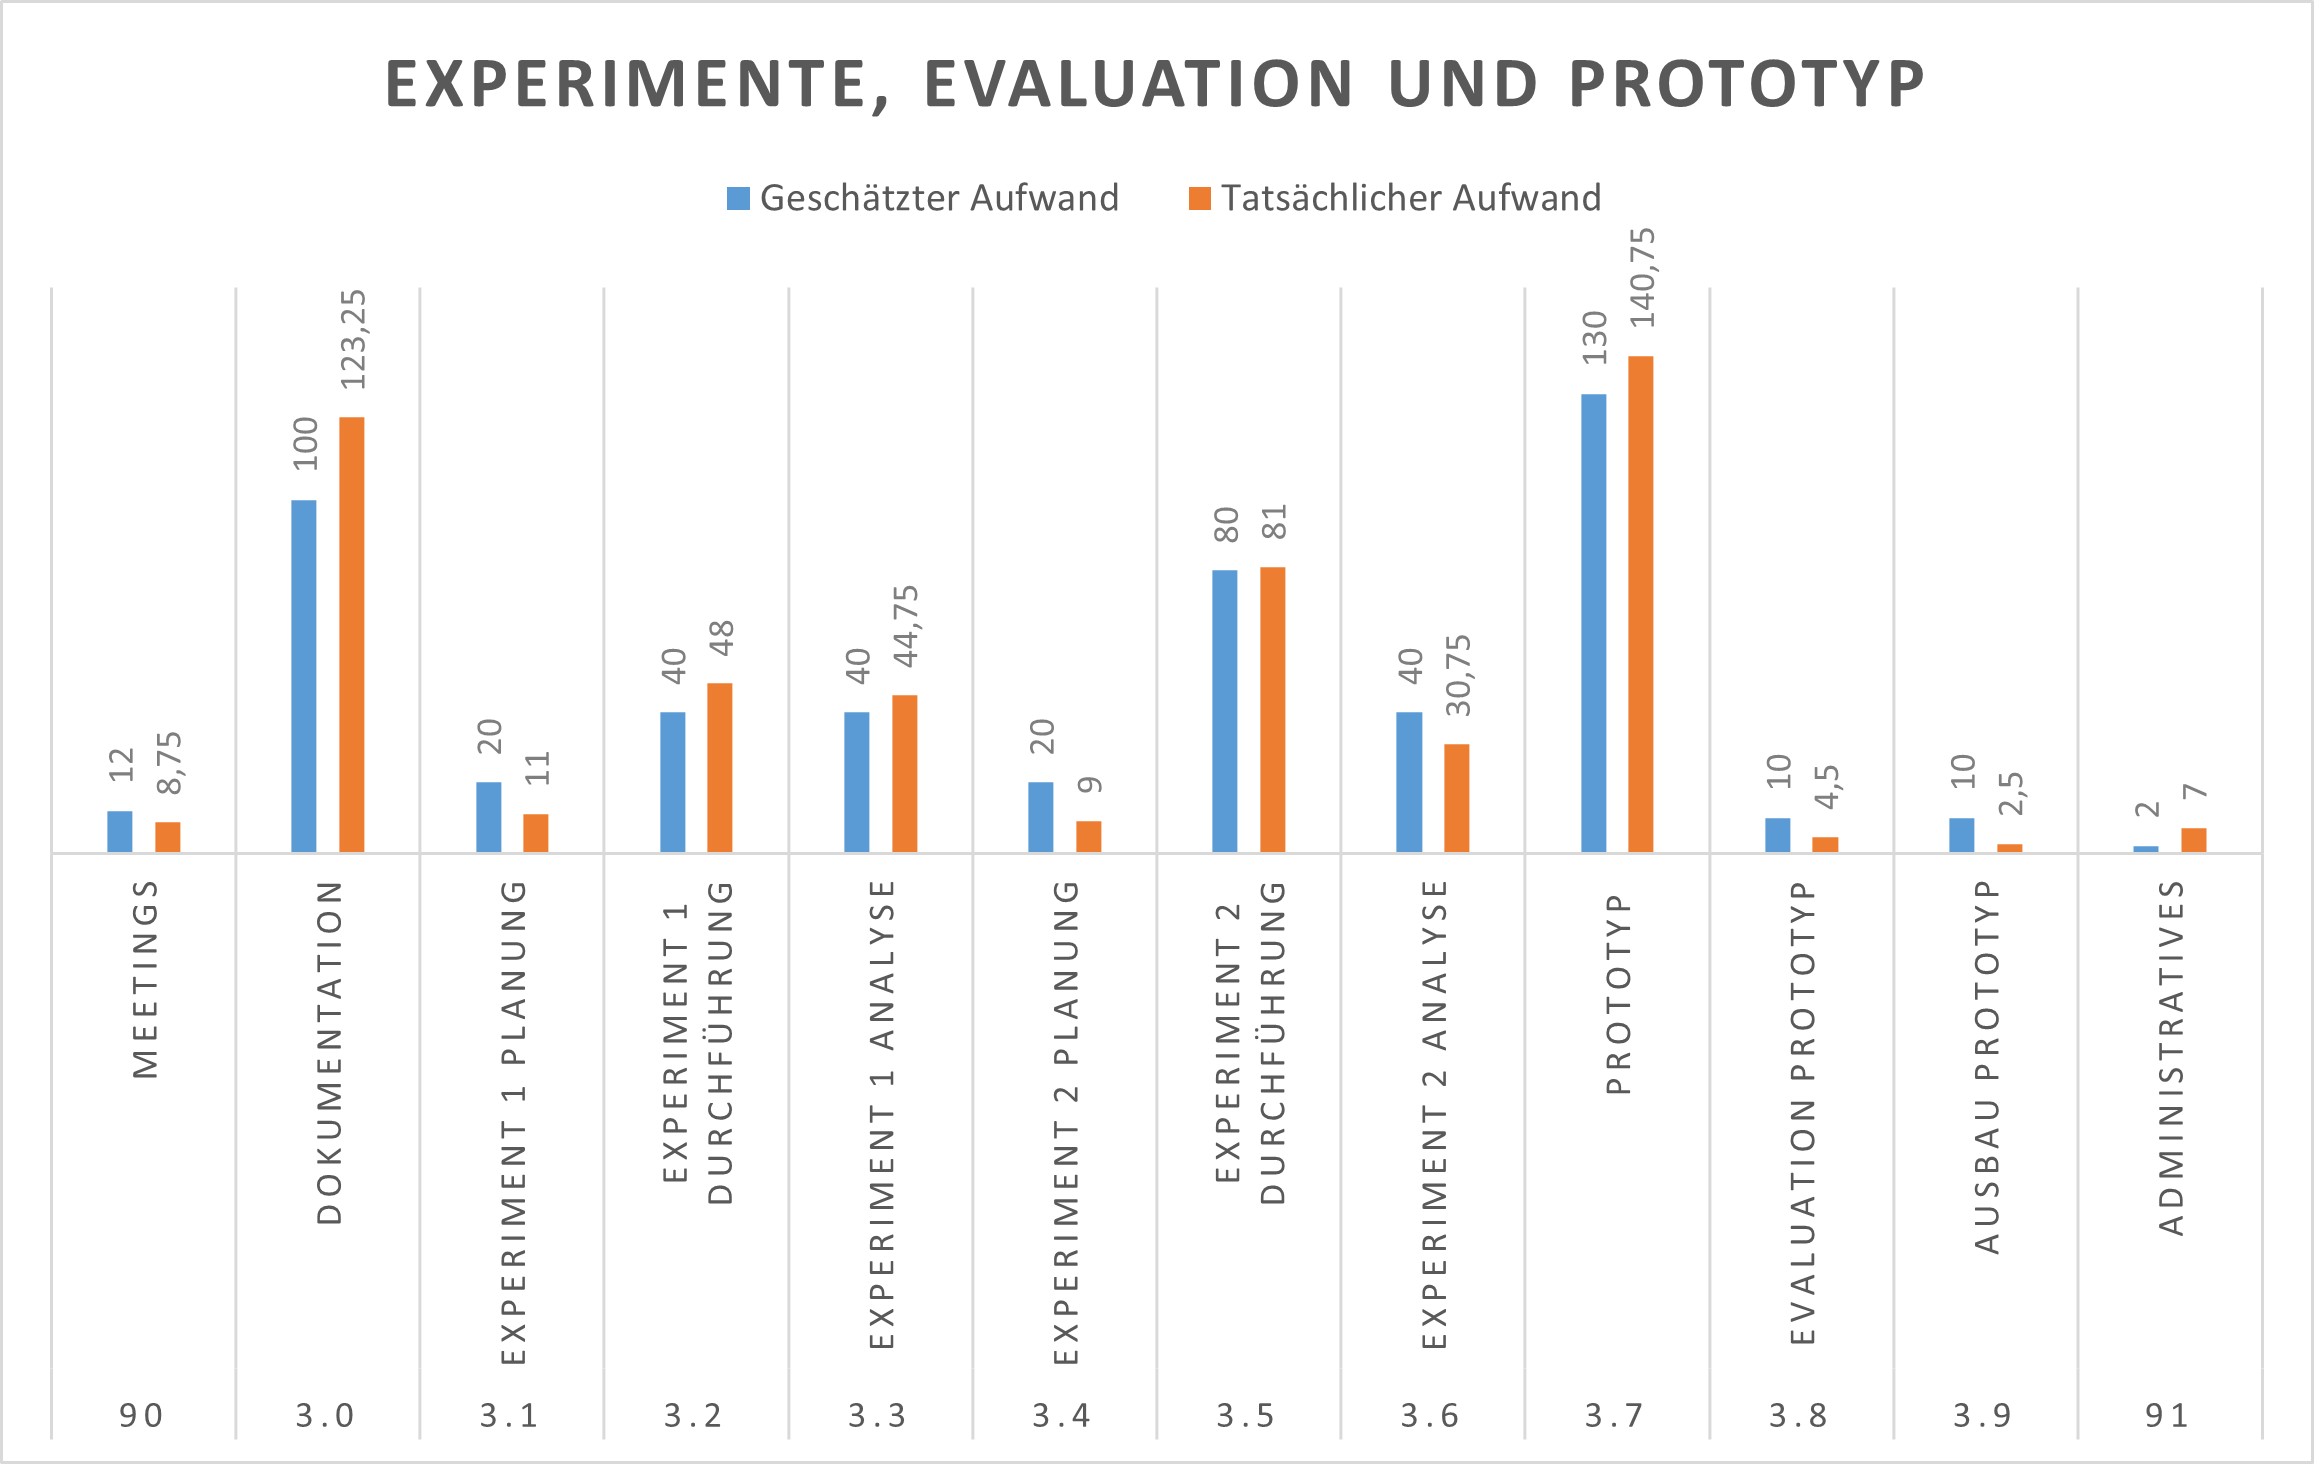
\includegraphics[width=1\linewidth]{Projectmanagement/EEP_Auswertung.png}
	\caption{Auswertung der Arbeitspakete in der dritten Phase
	\label{figure:eepevaluation}}
\end{figure}

Geplanter Aufwand: $504$ Stunden. \\
Tatsächlicher Aufwand: $511.25$ Stunden.

In der dritten Phase hatte es im Verlauf der Arbeit eine Änderung in der Planung 
gegeben. Die Android Messungen benötigten mehr Zeit als die iOS-Messungen. 
Im Meeting der Woche 7 wurde besprochen, dass die Messungen der Android-Geräte 
um eine Woche verlängert werden. Dadurch wurde die geschätzte Zeit für das 
Arbeitspaket von $40$ auf $80$ Stunden erhöht. Die Zeit wurde von den 
Arbeitspaketen Experiment 1 \& 2 Planung 
(zuvor je $40$ Stunden, danach $20$ Stunden) entfernt.

Vor allem die Arbeitspakete Dokumentation und Prototyp haben mehr Zeit 
beansprucht, als ursprünglich geplant. 

\clearpage 

\subsubsection*{Phase 4: Abschluss}
\begin{figure}[h!]
	\centering
	\includegraphics[width=1\linewidth]{Projectmanagement/Abschluss_Auswertung.png}
	\caption{Auswertung der Arbeitspakete in der Abschlussphase
	\label{figure:finishevaluation}}
\end{figure}

Geplanter Aufwand: $84$ Stunden. \\
Tatsächlicher Aufwand: $83.25$ Stunden.

\clearpage

\section{Infrastruktur 
\label{Infrastruktur}}
Beide Projektmitarbeiter verwenden ihre eigenen Notebooks mit Windows 10 
für die Durchführung der Bachelorarbeit. 
Weitere Hardware, die im Verlauf der Arbeit verwendet wird, 
wird fortlaufend dokumentiert.

\subsection*{Übersicht der Tools}
\begin{table}[H]
	\centering
	\begin{tabularx}{\linewidth}{l X}
		\toprule 
		\textbf{Bezeichnung} & \textbf{Verwendungsgrund} \\
		\midrule
		GitHub & Versionsverwaltung und Continuous Integration/Delivery \\
		GitKraken / SourceTree & Graphische Benutzeroberfläche für Git-Verwaltung \\
		Latex \& Visual Studio Code & Verfassung der Dokumentation \\
		Microsoft Excel & Zeiterfassung, Arbeitspakete und Spreadsheet-Auswertungen \\
		Whatsapp / Discord & Kommunikation innerhalb des Teams \\
		Microsoft Teams & Kommunikation mit dem Betreuer \\
		\bottomrule 
	\end{tabularx} 
	\caption{Übersicht der Tools
	\label{table:UebersichtTools}} 
\end{table}

\subsection*{Im Verlauf der Arbeit hinzugezogene Tools}
\begin{table}[H]
	\centering
	\begin{tabularx}{\linewidth}{l X}
		\toprule 
		\textbf{Bezeichnung} & \textbf{Verwendungsgrund} \\
		\midrule
		Wireshark & Messungen der Mobilgeräte \\
		\midrule
		Pycharm & Python Entwicklungsumgebung \\
		\bottomrule 
	\end{tabularx} 
	\caption{Hinzugezogene Tools
	\label{table:HinzugezogeneTools}} 
\end{table}

\clearpage 

\subsection*{Verwendete Hardware}
Die Tabelle~\ref{table:VerwendeteHardware} zeigt die in den Experimenten und
Prototypenentwicklung verwendete Hardware, den Gerätetypen und
den Hersteller. Mobilgeräte für die Messungen sind in den jeweiligen Abschnitten 
dokumentiert (iOS: Abschnitt~\ref{section:iosmeasurements} 
Tabelle~\ref{table:measurediosdevices}. 
Android: Abschnitt~\ref{section:androidmeasurements} 
Tabelle~\ref{table:measuredandroiddevices})
\begin{table}[H]
	\centering
	\begin{tabularx}{\linewidth}{l l l}
		\toprule 
		\textbf{Gerätebezeichnung} & \textbf{Gerätetyp} & \textbf{Hersteller} \\
		\midrule
		CAT S60 & Smartphone & Bullit Group \\
		\midrule 
		Macbook Pro & Laptop & Apple \\
		\midrule 
		WaveXpert & WLAN-Messgerät & Softing IT Networks GmbH  \\
		\bottomrule 
	\end{tabularx} 
	\caption{Verwendete Hardware
	\label{table:VerwendeteHardware}} 
\end{table}

\clearpage

\section{Qualitätsmassnahmen
\label{Qualitätsmassnahmen}}
Um für die Bachelorarbeit die Qualität zu gewährleisten, 
werden folgende Massnahmen getroffen:

\subsection*{Dokumentation}
Damit die Dokumentation über die Versionsverwaltung gemeinsam von allen 
Projektteilnehmern vorgenommen werden kann, wird ein Latex-Dokument 
aufgesetzt und über GitHub verwaltet.

\subsection*{Projektmanagement}
\subsubsection*{GitHub}
Für die Versionsverwaltung wird ein GitHub-Repository aufgesetzt. 
Im Bedarfsfall wird für die Umsetzung eines Prototyps eine Continuous 
Integration / Continuous Delivery Pipeline und allenfalls weitere 
Hilfsfunktionen konfiguriert.

Der main- und development-Branch sind beide so abgesichert, 
dass kein Projektteilnehmer direkt seine Änderung darauf Pushen kann, 
sondern die Anpassungen über einen Pull-Request eingibt. 
Dieser Request wird vom jeweils anderen Projektpartner kontrolliert 
und akzeptiert oder abgelehnt. Die Projektmitglieder verwenden für die 
Implementation jeweils spezifische Feature-Branches.

Diese Arbeitsweise erlaubt es, einen sicheren Arbeitsfluss zu gewährleisten, 
bei dem wenig Merge-Konflikte auftreten sollten und bei dem jede Änderung 
zuerst vom Partner durch ein Review abgesegnet werden muss, 
bevor sie integriert wird.

\subsubsection*{Prozessmodell}
Die Bachelorarbeit als Ganzes wird als Wasserfall-Modell aufgezogen. 
Der Beginn und das Ende der Arbeit sowie drei der Vier Projektphasen 
sind klar spezifiziert. 
Lediglich die dritte Phase wird als Iterative Phase durchgeführt, 
da im Vornherein nicht gesagt werden kann,
welche Resultate aus den Experimenten tatsächlich gewonnen werden können 
und ob diese Resultate für die Entwicklung eines Prototyps verwendet werden
können.

\clearpage 

\subsubsection*{Experimenteller Aufbau}
Damit die Experimente mit möglichst signifikanten Ergebnissen ausgeführt 
werden können, muss vor jeder Durchführung ein Plan mit den Parametern 
erstellt werden, wie genau das Experiment unter welchen Bedingungen 
durchgeführt wird, wie die zu erwartenden Ergebnisse aussehen und welche
Daten für die weitere Verwendung in welchem Format gespeichert werden sollen.
Nach den Experimenten müssen die Ergebnisse ausgewertet und dokumentiert werden. 
 
\part*{Anhang}
\addcontentsline{toc}{part}{Anhang}
\appendix
\frontmatter

% Glossary
% ====================
\chapter{Anhang A: Abkürzungsverzeichnis}
In der Tabelle~\ref{table:abreviationsandglossary} sind die in der Arbeit 
verwendeten Abkürzungen und deren Beschreibung dokumentiert.

\clearpage

\begin{longtable}{|l|l|}
    % Header on first page
    \hline
    \multicolumn{1}{|c|}{\textbf{Abkürzung}} & \multicolumn{1}{c|}{\textbf{Bezeichnung}} \\
    \hline
    \endfirsthead
    % Header on consecutive pages
    \hline 
    \multicolumn{2}{|c|}{{Fortführung der Tabelle}} \\
    \hline
    \multicolumn{1}{|c|}{\textbf{Abkürzung}} & \multicolumn{1}{c|}{\textbf{Bezeichnung}} \\
    \hline 
    \endhead
    % Footer to notify about continuation
    \hline 
    \multicolumn{2}{|c|}{{Tabelle wird auf der nächsten Seite fortgeführt}} \\
    \hline
    \endfoot
    \endlastfoot
    avg. & Average. Durchschnitt (-wert) \\
    \hline 
    AVT & Arbeitsverwaltungstool der OST-Schweizer Fachhochschule. \\
    \hline
    BSSID \& SSID & (Basic) Service Set ID. Für die Zuordnung von Geräten zu \\
    & einem Netzwerk. \\
    \hline
    CSV & Comma Separated Values. Datenformat mit kommaseparierten Einträgen \\
    \hline
    DS Parameter & Direct Sequence Parameter. Beschreibt vom Netzwerk \\
    & verwendeten WLAN-Kanal. \\
    \hline
    ECTS & European Credit Transfer and Accumulation System.\\
    & Standard für die Vergabe von akademischen Credits. \\
    \hline
    GHz \& MHz & Giga- \& Megahertz. Einheit für Frequenz. \\ 
    & Ein GHz ist 1000 MHz und 1 MHz ist 1000 Hz. \\
    \hline
    HT & Higher Throughput. 802.11n Erweiterung für höhere \\ 
    & Datendurchsätze. \\
    \hline
    A-MPDU & Aggregate MPDU. Verfahren im 802.11n Standard für die \\
    & Aggregation von MPDUs für erhöhten Datendurchsatz. \\
    \hline
    ICOM & Institut für Kommunikationssysteme der OST-Schweizer \\
    & Fachhochschule.\\
    \hline
    IE-Felder & Information-Element-Felder. Zusätzliche Geräteparameter,\\
    & die in Probe-Requests mitgesendet werden. \\
    \hline
    IEEE & Institute of Electrical and Electrionics Engineers. \\
    & Berufsverband von Elektroingenieuren welcher verschiedene \\
    & Standards herausgebracht hat. \\
    \hline
    IBAT & Inter-Burst-Arrival-Time. Zwischenankunftszeit von Bursts. \\
    \hline
    IFAT & Inter-Frame-Arrival-Time. Zwischenankunftszeit von Frames. \\
    \hline
    IFS & Institut für Software der OST-Schweizer Fachhochschule. \\
    \hline
    INS & Institute for Networked Solutions der OST-Schweizer \\
    & Fachhochschule. \\
    \hline
    iOS & Apple Betriebssystem. \\
    \hline
    IP & Internet-Protocol. Netzwerkprotokoll und Grundlage des \\
    & Internets. \\
    \hline
    JSON & Javascript Object Notation. Datenformat für den \\ 
    & Datenaustausch zwischen Anwendungen. \\
    % Page Break 
    MAC & Media Access Control. Adresse für den Medienzugriff \\
    & in der Netzwerktechnik. \\
    \hline
    MPDU & MAC Protocol Data Unit. Nachricht, die zwischen \\
    & MAC-Entitäten in Form von Frames ausgetauscht wird. \\
    \hline
    NIC & Network Interface Controller. Netzwerkkontroller- \\
    & spezifische Kennung für die eindeutige Identifikation \\ 
    & von Netzwerkkarten. \\
    \hline
    Nof & Number of. Anzahl von Entitäten. \\
    \hline
    OSI & Openn Systems Interconnection. Konzeptionelles Modell \\
    & für die standardisierung eine Computer Systems. \\
    \hline
    OUI & Organisational Unique Identifier. Herstellerspezifische \\
    & Kennung in der MAC-Adresse. \\
    \hline
    PNO \& ePNO & (Enhanced) Preferred Network Offload. Apple \\
    & Spezifikation für die Erkennung bekannter Netzwerke. \\
    \hline
    TCP & Transmission Control Protocol. Netzwerkprotokoll für die \\
    & Kommunikation über das Internet. \\
    \hline
    U/L Bit & Universal/Local Bit. Synonyme Bezeichnung für das \\
    & lokale Bit. \\
    \hline
    WEP & Wired Equivalent Privacy. Wi-Fi Standard für die \\
    & Netzwerksicherheit. \\
    \hline
    Wi-Fi & Wireless Fidelity. Protokoll für kabellose Netzwerke. \\
    & Oft als Synonym für WLAN verwendet. \\
    \hline
    WLAN & Wireless Local Area Network. Bezeichnung für ein \\ 
    & Kabelloses Computernetzwerk. \\
    \hline
    WPS & Wireless Protected Setup. Netzwerkstandard für schnelle \\
    & Verbindungen mit WLAN. \\
    \hline
    UUID & Universally Unique Identifier. 128-Bit ID für die eindeutige \\
    & Identifikation von Computersytemen oder -anwendungen. \\
    \hline
    \caption{Abkürzungen}  \label{table:abreviationsandglossary} \\
\end{longtable}

\clearpage 


% Bibliography
% ====================
\chapter{Anhang B: Quellenverzeichnis und Bibliografie}
Nachfolgend sind die in der Arbeit zitierten Quellen und die für die Recherche 
verwendete Bibliografie verzeichnet.

\clearpage

\section*{Quellenverzeichnis}

\subsection*{Paper: A Study of MAC Address Randomization.}
\begin{itemize}
    \item Name: Study of MAC Address Randomization in Mobile Devices and 
    When it Fails
    \item Autoren: Jeremy Martin, Travis Mayberry, Collin Donahue et al.
    \item Publikation: 2017, Proceedings on Privacy Enhancing Technologies 
\end{itemize}

\subsection*{Paper: Defeating MAC Address Randomization Through Timing Attacks}
\begin{itemize}
    \item Name: Defeating MAC Address Randomization Through Timing Attacks
    \item Autoren: Célestin Matte, Mathieu Cunche, Franck Rousseau et al.
    \item Publikation: 2016, WiSec Ausgabe Juli 2016
\end{itemize}

\subsection*{Paper: How Talkative is Your Mobile Device?}
\begin{itemize}
    \item Name: How Talkative is your Mobile Device? An Experimental Study of Wi-Fi 
    Probe-Requests
    \item Autoren: Julien Freudinger
    \item Publikation: 2015, WiSec Ausgabe Juni 2015
\end{itemize}

\subsection*{Paper: Noncooperative 802.11 MAC Layer Fingerprinting}
\begin{itemize}
    \item Name: Noncooperative 802.11 MAC Layer Fingerprinting and Tracking
    of Mobile Devices
    \item Autoren: Pieter Robyns, Bram Bonné, Peter Quax and Wim Lamotte
    \item Publikation: 2017, Hindawi Security and Communication Networks Volume 2017
\end{itemize}

\subsection*{Paper:Why MAC Address Randomization is not Enough}
\begin{itemize}
    \item Name: Why MAC Address Randomization is not Enough: 
    An Analysis of Wi-Fi Network Discovery Mechanisms
    \item Autoren: Mathy Vanhoef, Célestin Matte, Mathieu Cunche et al.
    \item Publikation: 2016, ASIA CSS Ausgabe 2016
\end{itemize}

\subsection*{Pyshark - Packet parser using wireshark's tshark}
\begin{itemize}
    \item Name: Pyshark Dokumentation
    \item Maintainer: KimiNewt
    \item URL \url{https://kiminewt.github.io/pyshark/}
\end{itemize}

\subsection*{Scapy}
\begin{itemize}
    \item Name: Scapy Dokumentation
    \item Autoren: Biondi Philippe
    \item URL: \url{https://scapy.readthedocs.io/en/latest/introduction.html}
\end{itemize}

\clearpage

\section*{Bibliografie}
 
Apple Inc. Use private Wi-Fi addresses in iOS 14, iPadOS 14, and \\ watchOS 7 \\
\url{https://support.apple.com/en-us/HT211227} \\
Abgerufen am 23.09.2020 \\
\newline
Apple Inc. iOS 14 Per-Network MAC Addresses \\
\url{https://developer.apple.com/forums/thread/651151} \\
Abgerufen am 23.09.2020 \\
\newline
Buberenko Volodymyr. Diving into Android Oreo security changes. \\
\url{https://uptech.team/blog/android-oreo-security-changes} \\
Abgerufen am 25.09.2020 \\
\newline
Buberenko Volodymyr. Android Oreo: all you need to know. \\
\url{https://uptech.team/blog/android-oreo-overview} \\
Abgerufen am 25.09.2020 \\
\newline
Cisco. Fundamentals of 802.11 Wireless Sniffing. \\
\url{https://www.cisco.com/c/en/us/support/docs/wireless-mobility/80211/200527-Fundamentals-of-802-11-Wireless-Sniffing.html} \\
Abgerufen am 03.10.2020 \\
\newline
David (Nachname Unbekannt). How to handle randomized MAC addresses on Android 9+ and iOS 14+. \\
\url{https://support.adamnet.works/t/how-to-handle-randomized-mac-addresses-on-android-9-and-ios-14/316} \\
Abgerufen am 29.09.2020 \\
\newline
Dorsey Brannon. The Perils of Probe Requests. \\
\url{https://medium.com/@brannondorsey/wi-fi-is-broken-3f6054210fa5} \\
Abgerufen am 30.09.2020 \\
\newline
Edwards Jim. Apple's New Anti-Tracking System For iPhones Doesn't Work, Researcher Claims.
\url{https://www.businessinsider.com/ios-8-mac-randomization-wifi-iphone-doesnt-work-2014-10} \\
Abgerufen am 22.09.2020 \\  
\clearpage 
Gast, Mathew S. 802.11 Wireless Networks: Chapter 4, 802.11 Framing in Detail.
Oreilly: \url{https://www.oreilly.com/library/view/80211-wireless-networks/0596100523/ch04.html} \\
\newline
Gast, Mathew S. 802.11 Wireless Networks: The Definitive Guide, 2nd Edition.
Oreilly: \url{https://www.oreilly.com/library/view/80211-wireless-networks/0596100523/} \\
\newline
Goodin Dan. Shielding MAC addresses from stalkers is hard and Android fails miserably at it.
\url{https://arstechnica.com/information-technology/2017/03/shielding-mac-addresses-from-stalkers-is-hard-android-is-failing-miserably/} \\
Abgerufen am 22.09.2020 \\ 
\newline
Google LLC. Privacy: MAC Randomization. \\
\url{https://source.android.com/devices/tech/connect/wifi-mac-randomization} \\
Abgerufen am 23.09.2020 \\ 
\newline
Google LLC. Android Enterprise Security White Paper. \\
\url{https://static.googleusercontent.com/media/www.android.com/de//static/2016/pdfs/enterprise/Android_Enterprise_Security_White_Paper_2019.pdf} \\
Abgerufen am 23.09.2020 \\
\newline
Harris Nik . Tracking People \& Devices with WiFi. \\
\url{https://nikharris.com/tracking-people/} \\
Abgerufen am 20.11.2020 \\
\newline
Hetting Claus. New ‘Private Address’ iPhone feature could severely impact the Wi-Fi industry, expert says.
\url{https://wifinowglobal.com/news-and-blog/new-private-wi-fi-address-iphone-feature-could-severely-impact-the-wi-fi-industry-expert-says/}\\
Abgerufen am 22.09.2020 \\
\newline
Jankie Michael. We analyse WWDC19. iOS 13 cracks down on location tracking.
\url{https://whatthe.fi/we-analyse-wwdc19-ios-13-cracks-down-on-location-tracking-4a4167b0d7d5} \\
Abgerufen am 23.09.2020 \\
\newline
Johannes (Nachname Unbekannt). MAC Address Randomization on iOS.
\url{https://www.turais.de/mac-address-randomization-on-ios-12/} \\
Abgerufen am 23.09.2020 \\
\clearpage 
Mamiit Aaron. Apple implements random MAC address on iOS 8. Goodbye, marketers.
\url{https://www.techtimes.com/articles/8233/20140612/apple-implements-random-mac-address-on-ios-8-goodbye-marketers.htm} \\
Abgerufen am 23.09.2020 \\
\newline
Nayanajith Rasika. CWAP 802.11- Probe Request/Response. \\
\url{https://mrncciew.com/2014/10/27/cwap-802-11-probe-requestresponse/} \\
Abgerufen am 10.10.2020 \\
\newline
Peterson Mike. iOS 14 MAC randomization privacy feature may cause Cisco enterprise network issues. \\
\url{https://appleinsider.com/articles/20/09/17/ios-14-mac-randomization-privacy-feature-may-cause-cisco-enterprise-network-issues} \\
Abgerufen am 01.10.2020 \\
\newline
Wikipedia. IEEE 802.11 - Channels and frequencies. \\
\url{https://en.wikipedia.org/wiki/IEEE_802.11#Channels_and_frequencies} \\
Abgerufen am 03.10.2020 \\


% List of figures
% ====================
\cleardoublepage
\renewcommand{\listfigurename}{Anhang C: Abbildungsverzeichnis}
\listoffigures

% List of tables
% ====================
\cleardoublepage
\renewcommand{\listtablename}{Anhang D: Tabellenverzeichnis}
\listoftables

\begin{landscape}
   \chapter{Anhang E: Experimentelle Daten
   \label{chapter:appendix:experimentaldata}}
   Die folgenden Tabellen beschreiben die Auswertung der Messergebnisse aus den Experimenten.
   Die Ergebnisse sind nach den einzelnen Mobilgeräten und -Versionen sortiert.

   \clearpage 

   \section*{iOS Messungen}
   \subsection*{iPhone 8, iOS-Version 14.0.1}
   \begin{table}[h!]
      \centering
      \begin{tabular}{|c|c|c|c|c|c|c|c|}
      \hline
      \textbf{Messung} & \textbf{Anzahl} & \textbf{Anzahl} & \textbf{min.} & \textbf{avg.} & \textbf{max.} & \textbf{Verpasste} & \textbf{Zwischen-}\\
      & \textbf{Probe Requests} & \textbf{Bursts} & \textbf{Burstgrösse} & \textbf{Burstgrösse} & \textbf{Burstgrösse} & \textbf{Frames} & \textbf{ankunftszeit}\\
      \hline
      Aktiv Lang & \phantom{0}384 & \phantom{0}86 & 1 & \phantom{0}4,465 & 18 & \phantom{0}241 & \phantom{0}42,16 s \\
      Passiv Lang & \phantom{00}71 & \phantom{0}29 & 1 & \phantom{0}2,448 & \phantom{0}6 & \phantom{0}129 & 126,83 s \\
      Verbunden Lang & \phantom{00}67 & \phantom{0}21 & 1 & \phantom{0}3,191 & \phantom{0}5 & \phantom{0}135 & 173,83 s \\
      Aktiv On On & \phantom{0}121 & \phantom{0}28 & 1 & \phantom{0}4,321 & 18 & \phantom{0}105 & \phantom{0}21,71 s \\
      Aktiv On Off & \phantom{00}72 & \phantom{0}23 & 1 & \phantom{0}3,130 & \phantom{0}8 & \phantom{0}100 & \phantom{0}21,52 s \\
      Passiv On On & \phantom{00}81 & \phantom{0}34 & 1 & \phantom{0}2,382 & \phantom{0}7 & \phantom{00}54 & \phantom{0}16,47 s \\
      Passiv On Off & \phantom{0}104 & \phantom{0}36 & 1 & \phantom{0}2,889 & \phantom{0}7 & \phantom{0}167 & \phantom{0}16,83 s \\
      Verbunden On On & \phantom{00}52 & \phantom{00}4 & 1 & 13,000 & 26 & \phantom{00}78 & 183,81 s \\
      Verbunden On Off & \phantom{00}23 & \phantom{00}5 & 1 & \phantom{0}4,600 & 12 & \phantom{00}35 & 136,39 s \\
      Hotspot Verfügbar & \phantom{00}66 & \phantom{0}15 & 1 & \phantom{0}4,400 & 18 & \phantom{00}34 & \phantom{0}38,58 s \\
      Flugmodus & \phantom{0}111 & \phantom{0}27 & 1 & \phantom{0}4,111 & \phantom{0}9 & \phantom{00}85 & \phantom{00}8,00 s \\
      Startup & \phantom{00}67 & \phantom{0}19 & 1 & \phantom{0}3,526 & \phantom{0}9 & \phantom{00}33 & \phantom{0}18,11 s \\
      \hline
      TOTAL & 1219 & 327 & 1 & \phantom{0}4,372 & 26 & 1196 & \phantom{0}67,02 s \\
      \hline
      \end{tabular}
      \caption{Ergebnisse iPhone 8 Messungen, iOS-Version 14
      \label{table:iphone8-14-results}} 
   \end{table}
   
   \clearpage 

   \subsection*{iPhone X - Raphael Jud, iOS-Version 14.0.1}
   \begin{table}[h!]
      \centering
      \begin{tabular}{|c|c|c|c|c|c|c|c|}
      \hline
      \textbf{Messung} & \textbf{Anzahl} & \textbf{Anzahl} & \textbf{min.} & \textbf{avg.} & \textbf{max.} & \textbf{Verpasste} & \textbf{Zwischen-}\\
      & \textbf{Probe Requests} & \textbf{Bursts} & \textbf{Burstgrösse} & \textbf{Burstgrösse} & \textbf{Burstgrösse} & \textbf{Frames} & \textbf{ankunftszeit}\\
      \hline
      Aktiv Lang & \phantom{0}222 & \phantom{0}90 & 1 & 2,467 & \phantom{0}8 & \phantom{0}206 & \phantom{0}40,05 s \\
      Passiv Lang & \phantom{0}587 & 161 & 1 & 3,646 & \phantom{0}7 & 1578 & \phantom{0}22,20 s \\
      Aktiv On On & \phantom{00}70 & \phantom{0}18 & 1 & 3,889 & 12 & \phantom{0}138 & \phantom{0}34,25 s \\
      Passiv On On & \phantom{0}102 & \phantom{0}19 & 1 & 5,368 & 10 & \phantom{0}236 & \phantom{0}27,54 s \\
      Verbunden On On & \phantom{00}10 & \phantom{00}3 & 2 & 3,333 & \phantom{0}4 & \phantom{00}10 & 192,56 s \\
      Hotspot Verfügbar & \phantom{00}79 & \phantom{0}18 & 2 & 4,389 & \phantom{0}8 & \phantom{0}214 & \phantom{0}33,03 s \\
      \hline
      TOTAL & 1070 & 309 & 1 & 3,849 & 12 & 2382 & \phantom{0}58,27 s\\
      \hline
      \end{tabular}
      \caption{Ergebnisse iPhone X Messungen, iOS-Version 14
      \label{table:iphoneXJud-14-results}} 
   \end{table}

   \clearpage 

   \subsection*{iPhone X, iOS-Version 12.3.1}
   \begin{table}[h!]
      \centering
      \begin{tabular}{|c|c|c|c|c|c|c|c|}
      \hline
      \textbf{Messung} & \textbf{Anzahl} & \textbf{Anzahl} & \textbf{min.} & \textbf{avg.} & \textbf{max.} & \textbf{Verpasste} & \textbf{Zwischen-}\\
      & \textbf{Probe Requests} & \textbf{Bursts} & \textbf{Burstgrösse} & \textbf{Burstgrösse} & \textbf{Burstgrösse} & \textbf{Frames} & \textbf{ankunftszeit}\\
      \hline
      Passiv Lang & \phantom{0}52 & \phantom{0}14 & 1 & 3,714 & \phantom{0}7 & \phantom{0}105 & 266,81 s \\
      Aktiv On On & \phantom{0}73 & \phantom{0}24 & 1 & 3,042 & \phantom{0}6 & \phantom{00}30 & \phantom{0}25,32 s \\
      Aktiv On Off & 141 & \phantom{0}41 & 2 & 3,439 & \phantom{0}7 & \phantom{0}231 & \phantom{0}14,70 s\\
      Passiv On On & 122 & \phantom{0}22 & 1 & 5,545 & 12 & \phantom{00}64 & \phantom{0}28,51 s \\
      Passiv On Off & \phantom{0}47 & \phantom{0}10 & 2 & 4,700 & \phantom{0}6 & \phantom{00}28 & \phantom{0}60,91 s \\
      Verbunden On On & 147 & \phantom{0}37 & 1 & 3,973 & \phantom{0}8 & \phantom{0}578 & \phantom{00}8,77 s \\
      Verbunden On Off & \phantom{0}81 & \phantom{0}20 & 1 & 4,050 & 12 & \phantom{0}638 & \phantom{00}8,88 s \\
      Flugmodus & \phantom{0}57 & \phantom{0}15 & 1 & 3,800 & \phantom{0}6 & \phantom{0}113 & \phantom{00}8,88 s \\
      Startup & \phantom{0}42 & \phantom{0}10 & 2 & 4,200 & \phantom{0}6 & \phantom{00}22 & \phantom{0}13,90 s \\
      \hline
      TOTAL & 762 & 193 & 1 & 4,051 & 12 & 1809 & \phantom{0}48,52 s\\
      \hline
      \end{tabular}
      \caption{Ergebnisse iPhone X Messungen, iOS-Version 12
      \label{table:iphoneX-12-results}} 
   \end{table}

   \clearpage 
      
   \subsection*{iPhone X, iOS-Version 14.0.1}
   \begin{table}[h!]
      \centering
      \begin{tabular}{|c|c|c|c|c|c|c|c|}
      \hline
      \textbf{Messung} & \textbf{Anzahl} & \textbf{Anzahl} & \textbf{min.} & \textbf{avg.} & \textbf{max.} & \textbf{Verpasste} & \textbf{Zwischen-}\\
      & \textbf{Probe Requests} & \textbf{Bursts} & \textbf{Burstgrösse} & \textbf{Burstgrösse} & \textbf{Burstgrösse} & \textbf{Frames} & \textbf{ankunftszeit}\\
      \hline
      Aktiv Lang  & \phantom{0}418 & 123 & 1 & 3,398 & 14 & \phantom{0}547 & \phantom{0}19,71 s \\
      Passiv Lang & \phantom{00}75 & \phantom{0}24 & 1 & 3,125 & \phantom{0}7 & \phantom{0}133 & 151,65 s \\
      Verbunden Lang & \phantom{00}58 & \phantom{0}57 & 2 & 4,526 & 18 & \phantom{0}489 & \phantom{0}47,06 s \\
      Aktiv On On & \phantom{0}107 & \phantom{0}21 & 1 & 5,095 & \phantom{0}9 & \phantom{0}145 & \phantom{0}29,64 s \\
      Aktiv On Off & \phantom{00}53 & \phantom{0}17 & 1 & 3,118 & \phantom{0}9 & \phantom{00}63 & \phantom{0}32,72 s \\
      Passiv On On & \phantom{00}75 & \phantom{0}16 & 1 & 4,688 & \phantom{0}7 & \phantom{0}158 & \phantom{0}36,60 s \\
      Passiv On Off & \phantom{00}89 & \phantom{0}20 & 1 & 4,450 & \phantom{0}8 & \phantom{00}64 & \phantom{0}29,80 s \\
      Verbunden On On & \phantom{0}229 & \phantom{0}47 & 1 & 4,872 & \phantom{0}9 & \phantom{0}302 & \phantom{0}12,15 s \\
      Verbunden On Off & \phantom{0}328 & \phantom{0}45 & 2 & 7,289 & 11 & \phantom{0}302 & \phantom{0}12,99 s \\
      Flugmodus & \phantom{00}76 & \phantom{0}15 & 1 & 5,067 & 10 & \phantom{00}44 & \phantom{00}9,91 s \\
      Startup & \phantom{00}76 & \phantom{0}15 & 2 & 5,067 & \phantom{0}9 & \phantom{00}73 & \phantom{0}14,08 s \\
      \hline
      TOTAL & 1784 & 400 & 1 & 4,607 & 18 & 2320 & \phantom{0}36,03 s \\
      \hline
      \end{tabular}
      \caption{Ergebnisse iPhone X Messungen, iOS-Version 14
      \label{table:iphoneX-14-results}} 
   \end{table}

   \clearpage

   \section*{Android Messungen}
   \subsection*{Samsung A51, Android Version 10}
   \begin{table}[h!]
      \centering
      \begin{tabular}{|c|c|c|c|c|c|c|c|}
      \hline
      \textbf{Messung} & \textbf{Anzahl} & \textbf{Anzahl} & \textbf{min.} & \textbf{avg.} & \textbf{max.} & \textbf{Verpasste} & \textbf{Zwischen-}\\
      & \textbf{Probe Requests} & \textbf{Bursts} & \textbf{Burstgrösse} & \textbf{Burstgrösse} & \textbf{Burstgrösse} & \textbf{Frames} & \textbf{ankunftszeit}\\
      \hline
      Aktiv Lang Mobile On & 115 & 19 & 2 & 6,053 & 12 & \phantom{0}92 & \phantom{0}168,11 \\
      Aktiv Lang Mobile Off & \phantom{0}14 & \phantom{0}3 & 2 & 4,667 & \phantom{0}8 & \phantom{0}13 & 1148,89 \\
      Passiv Lang Mobile On & \phantom{0}34 & \phantom{0}6 & 2 & 5,667 & 12 & \phantom{0}16 & \phantom{0}551,28 \\
      Passiv Lang Mobile Off & \phantom{0}25 & \phantom{0}4 & 3 & 6,250 & \phantom{0}8 & \phantom{0}26 & \phantom{0}369,40 \\
      Aktiv Mobile On & \phantom{0}28 & \phantom{0}1 & 4 & 7,000 & 11 & \phantom{0}10 & \phantom{00}35,16 \\
      Aktiv Mobile Off & \phantom{0}52 & \phantom{0}7 & 6 & 7,429 & \phantom{0}8 & \phantom{0}28 & \phantom{00}92,94 \\
      Passiv Mobile On & \phantom{0}30 & \phantom{0}5 & 3 & 6,000 & \phantom{0}8 & \phantom{0}20 & \phantom{0}104,54 \\
      Passiv Mobile Off & \phantom{0}21 & \phantom{0}3 & 6 & 7,000 & \phantom{0}8 & \phantom{0}11 & \phantom{0}272,61 \\
      Flugmodus & \phantom{0}32 & \phantom{0}5 & 3 & 6,400 & 11 & \phantom{0}21 & \phantom{000}8,15 \\
      Startup & \phantom{0}61 & \phantom{0}8 & 4 & 7,625 & 10 & \phantom{0}33 & \phantom{000}9,28 \\
      \hline 
      TOTAL & 412 & 61 & 2 & 6,409 & 12 & 270 & \phantom{0}276,04 \\
      \hline
      \end{tabular}
      \caption{Ergebnisse Samsung A51 Messungen, Android-Version 10
      \label{table:samsungA51-10-results}} 
   \end{table}

   \clearpage

   \subsection*{Samsung Galaxy S9, Android Version 10}
   \begin{table}[h!]
      \centering
      \begin{tabular}{|c|c|c|c|c|c|c|c|}
      \hline
      \textbf{Messung} & \textbf{Anzahl} & \textbf{Anzahl} & \textbf{min.} & \textbf{avg.} & \textbf{max.} & \textbf{Verpasste} & \textbf{Zwischen-}\\
      & \textbf{Probe Requests} & \textbf{Bursts} & \textbf{Burstgrösse} & \textbf{Burstgrösse} & \textbf{Burstgrösse} & \textbf{Frames} & \textbf{ankunftszeit}\\
      \hline
      Aktiv Lang On On & \phantom{0}98 & \phantom{0}36 & 1 & 2,722 & 6 & 230 & \phantom{0}100,33 \\
      Aktiv Lang On Off & 102 & \phantom{0}30 & 1 & 3,400 & 7 & 252 & \phantom{0}118,88 \\
      Passiv Lang On On & \phantom{00}5 & \phantom{00}3 & 1 & 1,667 & 3 & \phantom{00}5 & 1001,52 \\
      Verbunden   & 147 & \phantom{0}46 & 2 & 3,196 & 6 & \phantom{0}89 & \phantom{00}12,92 \\
      Flugmodus & \phantom{0}16 & \phantom{00}5 & 2 & 3,200 & 4 & \phantom{0}29 & \phantom{00}10,37 \\
      Startup & \phantom{0}16 & \phantom{00}5 & 2 & 3,200 & 5 & \phantom{0}27 & \phantom{00}27,26 \\
      \hline
      TOTAL & 384 & 125 & 1 & 2,897 & 7 & 632 & \phantom{0}211,88 \\
      \hline
      \end{tabular}
      \caption{Ergebnisse Samsung Galaxy S9 Messungen, Android-Version 10
      \label{table:samsunggalaxys9-10-results}} 
   \end{table}

   \clearpage

   \subsection*{Samsung Galaxy S20, Android Version 10}
   \begin{table}[h!]
      \small
      \centering
      \begin{tabular}{|c|c|c|c|c|c|c|c|}
      \hline
      \textbf{Messung} & \textbf{Anzahl} & \textbf{Anzahl} & \textbf{min.} & \textbf{avg.} & \textbf{max.} & \textbf{Verpasste} & \textbf{Zwischen-}\\
      & \textbf{Probe Requests} & \textbf{Bursts} & \textbf{Burstgrösse} & \textbf{Burstgrösse} & \textbf{Burstgrösse} & \textbf{Frames} & \textbf{ankunftszeit}\\
      \hline
      Aktiv Lang & \phantom{0}60 & \phantom{0}32 & 1 & 1,875 & 2 & \phantom{0}28 & 112,74 \\
      Passiv Lang 1 & 142 & 130 & 1 & 1,092 & 2 & \phantom{0}12 & \phantom{0}27,92 \\
      Passiv Lang 2 & \phantom{0}32 & \phantom{0}16 & 2 & 2,000 & 2 & \phantom{0}16 & 221,63 \\
      Verbunden Lang & \phantom{0}40 & \phantom{0}15 & 1 & 1,867 & 2 & \phantom{00}0 & 252,58 \\
      Aktiv 10 SSIDs On On & \phantom{0}10 & \phantom{00}5 & 2 & 2,000 & 2 & \phantom{00}5 & 125,59 \\
      Aktiv 10 SSIDs On Off & \phantom{0}26 & \phantom{0}13 & 2 & 2,000 & 2 & \phantom{0}13 & \phantom{0}37,95 \\
      Aktiv 5 SSIDs On Off & \phantom{0}60 & \phantom{0}30 & 2 & 2,000 & 2 & \phantom{0}30 & \phantom{0}18,53 \\
      Aktiv 1 SSIDs On On & \phantom{0}26 & \phantom{0}13 & 2 & 2,000 & 2 & \phantom{0}13 & \phantom{0}39,67 \\
      Aktiv 1 SSIDs On Off & \phantom{0}10 & \phantom{00}6 & 1 & 1,667 & 2 & \phantom{00}4 & 102,90 \\
      Passiv 10 SSIDs On On & \phantom{00}6 & \phantom{00}3 & 2 & 2,000 & 2 & \phantom{00}3 & 219,42 \\
      Passiv 10 SSIDs On Off & \phantom{00}7 & \phantom{00}4 & 1 & 1,750 & 2 & \phantom{00}3 & 116,26 \\
      Passiv 5 SSIDs On On & \phantom{00}8 & \phantom{00}4 & 2 & 2,000 & 2 & \phantom{00}4 & 141,44 \\
      Passiv 5 SSIDs On Off & \phantom{00}4 & \phantom{00}2 & 2 & 2,000 & 2 & \phantom{00}2 & 263,26 \\
      Passiv 1 SSIDs On On & \phantom{0}10 & \phantom{00}5 & 2 & 2,000 & 2 & \phantom{00}5 & 110,93 \\
      Passiv 1 SSIDs On Off & \phantom{00}6 & \phantom{00}3 & 2 & 2,000 & 2 & \phantom{00}3 & 180,52 \\
      Flugmodus & \phantom{0}26 & \phantom{0}14 & 1 & 1,857 & 2 & \phantom{0}12 & \phantom{0}16,45 \\
      Startup & \phantom{0}16 & \phantom{00}8 & 2 & 2,000 & 2 & \phantom{00}8 & \phantom{0}18,21 \\
      \hline
      TOTAL & 489 & 303 & 1 & 1,889 & 2 & 161 & 118,00 \\
      \hline
      \end{tabular}
      \caption{Ergebnisse Samsung Galaxy S20 Messungen, Android-Version 10
      \label{table:samsunggalaxys20-10-results}} 
   \end{table}

   \clearpage

   \subsection*{Google Pixel 3, Android Version 11}
   \begin{table}[h!]
      \small
      \centering
      \begin{tabular}{|c|c|c|c|c|c|c|c|}
      \hline
      \textbf{Messung} & \textbf{Anzahl} & \textbf{Anzahl} & \textbf{min.} & \textbf{avg.} & \textbf{max.} & \textbf{Verpasste} & \textbf{Zwischen-}\\
      & \textbf{Probe Requests} & \textbf{Bursts} & \textbf{Burstgrösse} & \textbf{Burstgrösse} & \textbf{Burstgrösse} & \textbf{Frames} & \textbf{ankunftszeit}\\
      \hline
      Aktiv Lang & 1785 & 375 & 1 & 4,760 & 11 & \phantom{0}568 & \phantom{00}9,52 \\
      Passiv Lang  & \phantom{0}271 & \phantom{0}59 & 2 & 4,593 & 11 & \phantom{0}133 & \phantom{0}61,86 \\
      Verbunden & \phantom{0}566 & \phantom{0}63 & 2 & 8,968 & 13 & \phantom{0}365 & \phantom{00}9,30 \\
      Aktiv 10 SSIDs On On & \phantom{0}364 & \phantom{0}69 & 1 & 5,275 & 10 & \phantom{0}127 & \phantom{00}8,72 \\
      Aktiv 10 SSIDs On Off & \phantom{00}93 & \phantom{0}22 & 1 & 4,227 & 10 & \phantom{00}45 & \phantom{0}28,77 \\
      Aktiv 5 SSIDs On On & \phantom{0}127 & \phantom{0}29 & 1 & 4,379 & 15 & \phantom{00}50 & \phantom{0}21,35 \\
      Aktiv 5 SSIDs On Off & \phantom{00}93 & \phantom{0}22 & 1 & 4,227 & 10 & \phantom{00}45 & \phantom{0}28,77 \\
      Aktiv 1 SSIDs On On & \phantom{0}320 & \phantom{0}63 & 1 & 5,079 & \phantom{0}9 & \phantom{0}128 & \phantom{00}9,57 \\
      Aktiv 1 SSIDs On Off & \phantom{0}261 & \phantom{0}66 & 1 & 3,955 & \phantom{0}9 & \phantom{0}113 & \phantom{00}9,21 \\
      Passiv 10 SSIDs On On & \phantom{00}17 & \phantom{0}13 & 1 & 1,308 & \phantom{0}5 & \phantom{000}1 & \phantom{0}45,36 \\
      Passiv 10 SSIDs On Off & \phantom{000}4 & \phantom{00}4 & 1 & 1,000 & \phantom{0}1 & \phantom{000}0 & 140,04 \\
      Passiv 5 SSIDs On On & \phantom{00}32 & \phantom{00}8 & 1 & 4,000 & 14 & \phantom{000}1 & \phantom{0}76,87 \\
      Passiv 5 SSIDs On Off & \phantom{00}11 & \phantom{0}11 & 1 & 1,000 & \phantom{0}1 & \phantom{000}0 & \phantom{0}56,03 \\
      Passiv 1 SSIDs On On & \phantom{0}428 & \phantom{0}72 & 1 & 5,944 & 10 & \phantom{0}236 & \phantom{00}8,32 \\
      Passiv 1 SSIDs On Off & \phantom{0}626 &\phantom{0} 71 & 1 & 8,817 & 14 & \phantom{0}249 & \phantom{00}8,23 \\
      Flugmodus & \phantom{00}33 & \phantom{00}8 & 2 & 4,125 & \phantom{0}7 & \phantom{00}12 & \phantom{0}14,64 \\
      Startup & \phantom{00}17 & \phantom{00}5 & 1 & 3,400 & \phantom{0}5 & \phantom{000}3 & \phantom{0}24,25 \\
      \hline
      TOTAL & 5048 & 960 & 1 & 4,415 & 15 & 2076 & \phantom{0}32,99 \\
      \hline
      \end{tabular}
      \caption{Ergebnisse Google Pixel 3 Messungen, Android-Version 11
      \label{table:googlepixel3-11-results}} 
   \end{table}

   \clearpage
   
   \subsection*{Samsung Galaxy S8 One, Android Version 9}
   \begin{table}[h!]
      \centering
      \begin{tabular}{|c|c|c|c|c|c|c|c|}
      \hline
      \textbf{Messung} & \textbf{Anzahl} & \textbf{Anzahl} & \textbf{min.} & \textbf{avg.} & \textbf{max.} & \textbf{Verpasste} & \textbf{Zwischen-}\\
      & \textbf{Probe Requests} & \textbf{Bursts} & \textbf{Burstgrösse} & \textbf{Burstgrösse} & \textbf{Burstgrösse} & \textbf{Frames} & \textbf{ankunftszeit}\\
      \hline
      Aktiv 20 min & 44 & 12 & 2 & 3,667 & 6 & 32 & 94,27 \\
      \hline
      \end{tabular}
      \caption{Ergebnisse Samsung Galaxy S8 (Erstes) Messungen, Android-Version 9
      \label{table:samsunggalaxys8-1-9-results}} 
   \end{table}

   \subsection*{Samsung Galaxy S8 Two, Android Version 9}
   \begin{table}[h!]
      \centering
      \begin{tabular}{|c|c|c|c|c|c|c|c|}
      \hline
      \textbf{Messung} & \textbf{Anzahl} & \textbf{Anzahl} & \textbf{min.} & \textbf{avg.} & \textbf{max.} & \textbf{Verpasste} & \textbf{Zwischen-}\\
      & \textbf{Probe Requests} & \textbf{Bursts} & \textbf{Burstgrösse} & \textbf{Burstgrösse} & \textbf{Burstgrösse} & \textbf{Frames} & \textbf{ankunftszeit}\\
      \hline
      Aktiv 20 min & 60 & 11 & 2 & 5,455 & 10 & 64 & 101,21 \\
      \hline
      \end{tabular}
      \caption{Ergebnisse Samsung Galaxy S8 (Zweites) Messungen, Android-Version 9
      \label{table:samsunggalaxys8-2-9-results}} 
   \end{table}
   
   \clearpage

   \subsection*{Samsung Galaxy S8 Three, Android Version 9}
   \begin{table}[h!]
      \centering
      \begin{tabular}{|c|c|c|c|c|c|c|c|}
      \hline
      \textbf{Messung} & \textbf{Anzahl} & \textbf{Anzahl} & \textbf{min.} & \textbf{avg.} & \textbf{max.} & \textbf{Verpasste} & \textbf{Zwischen-}\\
      & \textbf{Probe Requests} & \textbf{Bursts} & \textbf{Burstgrösse} & \textbf{Burstgrösse} & \textbf{Burstgrösse} & \textbf{Frames} & \textbf{ankunftszeit}\\
      \hline
      Aktiv 20 min & 149 & 20 & 1 & 7,450 & 13 & 149 & 55,78 \\
      \hline
      \end{tabular}
      \caption{Ergebnisse Samsung Galaxy S8 (Drittes) Messungen, Android-Version 9
      \label{table:samsunggalaxys8-3-9-results}} 
   \end{table}

   \subsection*{Samsung Galaxy S8 Four, Android Version 9}
   \begin{table}[h!]
      \centering
      \begin{tabular}{|c|c|c|c|c|c|c|c|}
      \hline
      \textbf{Messung} & \textbf{Anzahl} & \textbf{Anzahl} & \textbf{min.} & \textbf{avg.} & \textbf{max.} & \textbf{Verpasste} & \textbf{Zwischen-}\\
      & \textbf{Probe Requests} & \textbf{Bursts} & \textbf{Burstgrösse} & \textbf{Burstgrösse} & \textbf{Burstgrösse} & \textbf{Frames} & \textbf{ankunftszeit}\\
      \hline
      Aktiv 20 min & 101 & 14 & 4 & 7,214 & 11 & 200 & 80,29 \\
      \hline
      \end{tabular}
      \caption{Ergebnisse Samsung Galaxy S8 (Viertes) Messungen, Android-Version 9
      \label{table:samsunggalaxys8-4-9-results}} 
   \end{table}

   \clearpage

   \subsection*{Fairphone 3+, Android Version 10}
   \begin{table}[h!]
      \small
      \centering
      \begin{tabular}{|c|c|c|c|c|c|c|c|}
      \hline
      \textbf{Messung} & \textbf{Anzahl} & \textbf{Anzahl} & \textbf{min.} & \textbf{avg.} & \textbf{max.} & \textbf{Verpasste} & \textbf{Zwischen-}\\
      & \textbf{Probe Requests} & \textbf{Bursts} & \textbf{Burstgrösse} & \textbf{Burstgrösse} & \textbf{Burstgrösse} & \textbf{Frames} & \textbf{ankunftszeit}\\
      \hline
      Aktiv Lang Macbook & \phantom{0}308 & \phantom{0}52 & \phantom{0}1 & \phantom{0}5,923 & 17 & 152 & \phantom{0}69,53 \\
      Aktiv Lang WaveXpert & \phantom{0}251 & \phantom{0}22 & \phantom{0}7 & 11,409 & 19 & 61 & 124,61 \\
      Passiv Lang Macbook & \phantom{0}112 & \phantom{0}56 & \phantom{0}2 & \phantom{0}2,000 & \phantom{0}2 & \phantom{00}0 & \phantom{0}63,28 \\
      Passiv Lang WaveXpert & \phantom{0}110 & \phantom{0}56 & \phantom{0}1 & \phantom{0}1,964 & \phantom{0}2 & \phantom{00}0 & \phantom{0}63,28 \\
      Verbungen Lang & \phantom{0}407 & \phantom{0}28 & \phantom{0}1 & 12,893 & 20 & 134 & 130,54 \\
      Aktiv Ohne Sim 30 min & \phantom{0}209 & \phantom{0}12 & \phantom{0}1 & 10,083 & 14 & \phantom{0}35 & 153,74 \\
      Aktiv 10 SSIDs & \phantom{00}64 & \phantom{00}5 & 10 & 12,800 & 16 & \phantom{0}20 & 122,58 \\
      Aktiv 5 SSIDs & \phantom{00}64 & \phantom{00}4 & 15 & 15,750 & 16 & \phantom{0}18 & 159,75 \\
      Aktiv 0 SSIDs & \phantom{00}60 & \phantom{00}4 & 14 & 15,000 & 16 & \phantom{0}17 & 159,81 \\
      Aktiv On On & \phantom{0}112 & \phantom{00}7 & \phantom{0}1 & 16,000 & 25 & \phantom{0}72 & \phantom{0}92,37 \\
      Aktiv On Off & \phantom{00}55 & \phantom{00}3 & 14 & 18,000 & 21 & \phantom{0}29 & 225,49 \\
      Passiv On On & \phantom{00}64 & \phantom{0}54 & \phantom{0}1 & \phantom{0}1,185 & \phantom{0}2 & \phantom{00}0 & \phantom{0}10,75 \\
      Passiv On Off & \phantom{00}79 & \phantom{0}52 & \phantom{0}1 & \phantom{0}1,500 & 17 & \phantom{00}4 & \phantom{00}9,76 \\
      5GHz Messung & \phantom{0}267 & \phantom{0}19 & \phantom{0}1 & 12,053 & 18 & 122 & \phantom{0}65,11 \\
      Flugmodus & \phantom{00}72 & \phantom{00}5 & 11 & 14,400 & 18 & \phantom{0}45 & \phantom{0}10,87 \\
      Startup & \phantom{00}95 & \phantom{00}7 & \phantom{0}9 & 13,571 & 19 & \phantom{0}35 & \phantom{0}37,58 \\
      \hline 
      TOTAL & 2329 & 386 & \phantom{0}1 & 10,283 & 25 & 744 & \phantom{0}93,69 \\
      \hline
      \end{tabular}
      \caption{Ergebnisse Fairphone 3+ Messungen, Android-Version 10
      \label{table:fairphone3-10-results}} 
   \end{table}

   \clearpage
         
\end{landscape}


\chapter{Anhang F: Verhaltenskatalog der Mobilgeräte}
In den folgenden Abschnitten ist das Verhalten der einzelnen Mobilgeräte 
aus den Messungen in Form eines Gerätekatalogs beschrieben.

\clearpage 
\section*{Android-Geräte}
\subsection*{Samsung A51}
Generelle Informationen zu den Messungen:

\begin{table}[h!]
    \begin{tabularx}{\textwidth}{l X }
        \toprule
        Android Version & 10 \\
        Anzahl gemessene Bursts & 61 \\
        Bursts pro Minute & 0.47 \\
        Min Burst Grösse & 2 \\
        Max Burst Grösse & 12 \\
        Avg Burst Grösse & 6.4 \\
        Avg Inter-Burst-Arrival-Time & 276.04 \\
        \bottomrule
    \end{tabularx}
\end{table}

Verhalten des Gerätes:

\begin{table}[h!]
    \begin{tabularx}{\textwidth}{l X }
        \toprule
        Sequenz Nummer & Nicht Randomisiert \\
        \midrule
        Local Bit & Immer Gesetzt \\
        \midrule
        IE-Felder & \begin{itemize}
            \item 0 : SSID
            \item 1 : Supported Rates
            \item 50 : Extended Supported Rates
            \item 3 : DS Parameters
            \item 45 : HT Capabilities
            \item 127 : Extended Capabilities
            \item 221 : Microsoft Corp.
        \end{itemize} \\
        \midrule
        Spezielles Verhalten & Das Samsung A51 sendet die Bursts immer mit der gleichen MAC-Adresse \\
        \bottomrule
    \end{tabularx}
\end{table}
\clearpage


\subsection*{Samsung Galaxy S9}
Generelle Informationen zu den Messungen:

\begin{table}[h!]
    \begin{tabularx}{\textwidth}{l X }
        \toprule
        Android Version & 10 \\
        Anzahl gemessene Bursts & 125 \\
        Bursts pro Minute & 0.65 \\
        Min Burst Grösse & 1 \\
        Max Burst Grösse & 7 \\
        Avg Burst Grösse & 2.897 \\
        Avg Inter-Burst-Arrival-Time & 211.88 \\
        \bottomrule
    \end{tabularx}
\end{table}

Verhalten des Gerätes:

\begin{table}[h!]
    \begin{tabularx}{\textwidth}{l X }
        \toprule
        Sequenz Nummer & Randomisiert \\
        \midrule
        Local Bit & Immer Gesetzt \\
        \midrule
        IE-Felder & \begin{itemize}
            \item 0 : SSID
            \item 1 : Supported Rates
            \item 50 : Extended Supported Rates
            \item 3 : DS Parameters
            \item 45 : HT Capabilities
            \item 127 : Extended Capabilities
            \item 221 : Epigram, Inc.
            \item 221 : Microsoft Corp.
            \item 221 : Broadcom
            \item 221 : Epigram, Inc.
        \end{itemize} \\
        \midrule
        Spezielles Verhalten & - \\
        \bottomrule
    \end{tabularx}
\end{table}
\clearpage


\subsection*{Samsung Galaxy S20}
Generelle Informationen zu den Messungen:

\begin{table}[h!]
    \begin{tabularx}{\textwidth}{l X }
        \toprule
        Android Version & 10 \\
        Anzahl gemessene Bursts & 303 \\
        Bursts pro Minute & 0.97 \\
        Min Burst Grösse & 1 \\
        Max Burst Grösse & 2 \\
        Avg Burst Grösse & 1.889 \\
        Avg Inter-Burst-Arrival-Time & 118 \\
        \bottomrule
    \end{tabularx}
\end{table}

Verhalten des Gerätes:

\begin{table}[h!]
    \begin{tabularx}{\textwidth}{l X }
        \toprule
        Sequenz Nummer & Randomisiert \\
        \midrule
        Local Bit & Immer Gesetzt \\
        \midrule
        IE-Felder & \begin{itemize}
            \item 0 : SSID
            \item 1 : Supported Rates
            \item 50 : Extended Supported Rates
            \item 3 : DS Parameters
            \item 45 : HT Capabilities
            \item 127 : Extended Capabilities
            \item 255 : FILS Req. Params.
            \item 255 : HE Capabilities
            \item 221 : Epigram, Inc.
            \item 221 : Microsoft Corp.
            \item 221 : Broadcom
            \item 221 : Wi-Fi - Alliance
        \end{itemize} \\
        \midrule
        Spezielles Verhalten & Das Samsung Galaxy S20 sendet in der Regel Bursts mit der Grösse 2 \\
        \bottomrule
    \end{tabularx}
\end{table}
\clearpage


\subsection*{Google Pixel 3}
Generelle Informationen zu den Messungen:

\begin{table}[h!]
    \begin{tabularx}{\textwidth}{l X }
        \toprule
        Android Version & 11 \\
        Anzahl gemessene Bursts & 960 \\
        Bursts pro Minute & 3.29 \\
        Min Burst Grösse & 1 \\
        Max Burst Grösse & 15 \\
        Avg Burst Grösse & 4.415 \\
        Avg Inter-Burst-Arrival-Time & 32.99 \\
        \bottomrule
    \end{tabularx}
\end{table}

Verhalten des Gerätes:

\begin{table}[h!]
    \begin{tabularx}{\textwidth}{l X }
        \toprule
        Sequenz Nummer & Randomisiert \\
        \midrule
        Local Bit & Immer Gesetzt \\
        \midrule
        IE-Felder & \begin{itemize}
            \item 0 : SSID
            \item 1 : Supported Rates
            \item 50 : Extended Supported Rates
            \item 3 : DS Parameters
            \item 221 : Microsoft Corp.
            \item 221 : Wi-Fi - Alliance
        \end{itemize} \\
        \midrule
        Spezielles Verhalten & Das Pixel 3 sendet mehr Bursts als alle anderen gemessenen Geräte. \\
        \bottomrule
    \end{tabularx}
\end{table}
\clearpage


\subsection*{Fairphone 3}
Generelle Informationen zu den Messungen:

\begin{table}[h!]
    \begin{tabularx}{\textwidth}{l X }
        \toprule
        Android Version & 10\\
        Anzahl gemessene Bursts & 386 \\
        Bursts pro Minute & 1.26 \\
        Min Burst Grösse & 1 \\
        Max Burst Grösse & 25 \\
        Avg Burst Grösse & 10.293 \\
        Avg Inter-Burst-Arrival-Time & 93.69 \\
        \bottomrule
    \end{tabularx}
\end{table}

Verhalten des Gerätes:

\begin{table}[h!]
    \begin{tabularx}{\textwidth}{l X }
        \toprule
        Sequenz Nummer & Nicht Randomisiert \\
        \midrule
        Local Bit & Immer Gesetzt \\
        \midrule
        IE-Felder & \begin{itemize}
            \item 0 : SSID
            \item 1 : Supported Rates
            \item 50 : Extended Supported Rates
            \item 3 : DS Parameters [ca. 70\%]
            \item 45 : HT Capabilities [ca. 70\%]
            \item 221 : Microsoft Corp. [ca. 70\%]
        \end{itemize} \\
        \midrule
        Spezielles Verhalten & Das Pixel 3 sendet mehr Bursts als alle anderen gemessenen Geräte. \\
        \bottomrule
    \end{tabularx}
\end{table}
\clearpage

\section*{Apple-Geräte}

\subsection*{iPhone 8}
Generelle Informationen zu den Messungen:

\begin{table}[h!]
    \begin{tabularx}{\textwidth}{l X }
        \toprule
        iOS Version & 14.0.1\\
        Anzahl gemessene Bursts & 327 \\
        Bursts pro Minute & 2.16 \\
        Min Burst Grösse & 1 \\
        Max Burst Grösse & 26 \\
        Avg Burst Grösse & 4.372 \\
        Avg Inter-Burst-Arrival-Time & 62.02 \\
        \bottomrule
    \end{tabularx}
\end{table}

Verhalten des Gerätes:

\begin{table}[h!]
    \begin{tabularx}{\textwidth}{l X }
        \toprule
        Sequenz Nummer & Randomisiert \\
        \midrule
        Local Bit & Randomisiert \\
        \midrule
        IE-Felder & \begin{itemize}
            \item 0 : SSID
            \item 1 : Supported Rates
            \item 50 : Extended Supported Rates
            \item 3 : DS Parameters
            \item 45 : HT Capabilities 
            \item 127 : Extended Capabilities
            \item 107 : Interworking [ca. 25\%]
            \item 221 : Apple [ca. 45\%]
            \item 221 : Microsoft Corp. [ca. 45\%]
            \item 221 : Broadcom [ca. 45\%]
        \end{itemize} \\
        \midrule
        Spezielles Verhalten & - \\
        \bottomrule
    \end{tabularx}
\end{table}
\clearpage


\subsection*{iPhone X}
Generelle Informationen zu den Messungen:

\begin{table}[h!]
    \begin{tabularx}{\textwidth}{l X }
        \toprule
        iOS Version & 14.0.1\\
        Anzahl gemessene Bursts & 309 \\
        Bursts pro Minute & 1.66 \\
        Min Burst Grösse & 1 \\
        Max Burst Grösse & 12 \\
        Avg Burst Grösse & 3.849 \\
        Avg Inter-Burst-Arrival-Time & 58.27 \\
        \bottomrule
    \end{tabularx}
\end{table}

Verhalten des Gerätes:

\begin{table}[h!]
    \begin{tabularx}{\textwidth}{l X }
        \toprule
        Sequenz Nummer & Randomisiert \\
        \midrule
        Local Bit & Randomisiert \\
        \midrule
        IE-Felder & \begin{itemize}
            \item 0 : SSID
            \item 1 : Supported Rates
            \item 50 : Extended Supported Rates
            \item 3 : DS Parameters
            \item 45 : HT Capabilities 
            \item 127 : Extended Capabilities
            \item 107 : Interworking [ca. 5\%]
        \end{itemize} \\
        \midrule
        Spezielles Verhalten & - \\
        \bottomrule
    \end{tabularx}
\end{table}
\clearpage




\chapter{Anhang G: Risikotabelle}
In den nachfolgenden Unterabschnitten sind der Projektplan, jeweils zum Beginn 
der Bachelorarbeit und zum Ende der Bachelorarbeit abgelegt.
\begin{landscape}
\begin{table}[h!]
    \tiny  
	\centering
	\begin{tabularx}{\linewidth}{l l l l l X X X}
        \toprule 
        \multirow{2}{*}{\textbf{Nr}} & \multirow{2}{*}{\textbf{Titel}} & \textbf{Maximaler} & \textbf{Eintrittswahr-} & \textbf{Gewichteter}   & \multirow{2}{*}{\textbf{Vorbeugung}} & \textbf{Verhalten beim}  & \multirow{2}{*}{\textbf{Risikoabdeckung }}\\
        & & \textbf{Schaden [h]} & \textbf{scheinlichkeit} & \textbf{Schaden} & & \textbf{Eintreten}  & \\
        \midrule 
        R1 & Testgeräte & 10 & 10\% & 1 & Genaue Planung, welche Geräte benötigt werden und wie diese beschafft werden können & Anpassen der Gerätespezifikationen und beschaffung über weitere Quellen (Ausleihen von Instituten, Kollegen, Familie) & Genaue Spezifikation der benötigten Geräte und -betriebssysteme. Frühe beschaffung durch Projektteilnehmer und -Betreuer \\ 
        \midrule 
        R2 & Testvorbereitung & 20 & 25\% & 5 & Genaue Spezifizierung von Testparametern, bevor der Versuchsaufbau stattfindet & Testspezifikationen müssen überarbeitet werden. & Verifizieren, dass Versuchsaufbau durchführbar ist und zu den erwarteten Ergebnissen führt. Abklären des Aufbaus mit Experten. \\ 
        \midrule 
        R3 & Testdurchführung & 40 & 15\% & 6 & Testgeräte genau auf den Versuchsaufbau vorbereiten, genaue Testspezifikationen. Sicherstellen durch periodische Überprüfung, dass laufende Tests die Betriebsparameter erfüllen & Der gesamte Test oder Teile davon müssen erneut durchgeführt werden. & Versuchsaufbau unter kontrollierten Bedingungen. Periodisches Überprüfen nach jedem Versuchsschritt, dass keine Fehler vorgekommen sind \\ 
        \midrule 
        R4 & Testauswertung  & 42 & 10\% & 4,2 & Erwartete Resultate in der Versuchsplanung definieren und bei der Durchführung kontrollieren & Versuchsaufbau anpassen und Tests wiederholen & Risiko lässt sich mitigieren, indem die Gerätespezifikation im vornherein sehr genau studiert wird und die erwarteten Ergebnisse in der Versuchsplanung definiert werden \\ 
        \midrule 
        R5 & Format Versuchsdaten & 60 & 15\% & 9 & Datenformat und Erwartete Resultate in der Testplanung spezifizieren. Vorbereiten der Testdokumentation & Versuche müssen wiederholt werden & Recherche, welche Formate und Speichermöglichkeiten sich am besten für die Versuche eignen. \\ 
        \midrule 
        R6 & Gerätemerkmale & 100 & 20\% & 20 & Recherchen, um vorab zu wissen, wie sich die Mobilgeräte verhalten & Abklären mit Betreuer, ob die Aufgabenstellung der BA an die Erkenntnisse angepasst werden muss. & Höhere Anzahl Messungen und genau spezifizierte erwartete Messergebnisse \\ 
        \midrule 
        R7 & Geräteverhalten & 40 & 15\% & 6 & Mehrere Messungen mit gleichem Gerätetyp und OS-Version, um Abweichungen zu erkennen. & Mehr Geräte organisieren und weitere Versuche anstellen & Messungen mit unterschiedlichen Gerätetypen und verschiedenen Betriebssystemversionen \\ 
        \midrule 
        R8 & Hardwareverhalten & 42 & 10\% & 4.2 & Mehrere Messungen mit identischem OS auf unterschiedlicher HW durchführen & Mehr Geräte organisieren und weitere Versuche anstellen & Mehrere Geräte mit identischem OS verwenden \\
		\bottomrule 
	\end{tabularx} 
	\caption{Risikotabelle Projektbeginn
	\label{table:riskbeginn}} 
\end{table}

\clearpage 

\begin{table}[h!]
    \tiny  
	\centering
	\begin{tabularx}{\linewidth}{l l l l l X X X}
		\toprule 
        \multirow{2}{*}{\textbf{Nr}} & \multirow{2}{*}{\textbf{Titel}} & \textbf{Maximaler} & \textbf{Eintrittswahr-} & \textbf{Gewichteter}   & \multirow{2}{*}{\textbf{Vorbeugung}} & \textbf{Verhalten beim}  & \multirow{2}{*}{\textbf{Risikoabdeckung }}\\
        & & \textbf{Schaden [h]} & \textbf{scheinlichkeit} & \textbf{Schaden} & & \textbf{Eintreten}  & \\
        \midrule 
        R1 & Testgeräte & 5 & 5\% & 0,25 & Genaue Planung, welche Geräte benötigt werden und wie diese beschafft werden können & Anpassen der Gerätespezifikationen und beschaffung über weitere Quellen (Ausleihen von Instituten, Kollegen, Familie) & Genaue Spezifikation der benötigten Geräte und -betriebssysteme. Frühe beschaffung durch Projektteilnehmer und -Betreuer \\ 
        \midrule 
        R2 & Testvorbereitung & 10 & 10\% & 1 & Genaue Spezifizierung von Testparametern, bevor der Versuchsaufbau stattfindet & Testspezifikationen müssen überarbeitet werden. & Verifizieren, dass Versuchsaufbau durchführbar ist und zu den erwarteten Ergebnissen führt. Abklären des Aufbaus mit Experten. \\ 
        \midrule 
        R3 & Testdurchführung & 30 & 10\% & 3 & Testgeräte genau auf den Versuchsaufbau vorbereiten, genaue Testspezifikationen. Sicherstellen durch periodische Überprüfung, dass laufende Tests die Betriebsparameter erfüllen & Der gesamte Test oder Teile davon müssen erneut durchgeführt werden. & Versuchsaufbau unter kontrollierten Bedingungen. Periodisches Überprüfen nach jedem Versuchsschritt, dass keine Fehler vorgekommen sind \\ 
        \midrule 
        R4 & Testauswertung  & 42 & 5\% & 2,1 & Erwartete Resultate in der Versuchsplanung definieren und bei der Durchführung kontrollieren & Versuchsaufbau anpassen und Tests wiederholen & Risiko lässt sich mitigieren, indem die Gerätespezifikation im vornherein sehr genau studiert wird und die erwarteten Ergebnisse in der Versuchsplanung definiert werden \\ 
        \midrule 
        R5 & Format Versuchsdaten & 60 & 5\% & 3 & Datenformat und Erwartete Resultate in der Testplanung spezifizieren. Vorbereiten der Testdokumentation & Versuche müssen wiederholt werden & Recherche, welche Formate und Speichermöglichkeiten sich am besten für die Versuche eignen. \\ 
        \midrule 
        R6 & Gerätemerkmale & 80 & 20\% & 16 & Recherchen, um vorab zu wissen, wie sich die Mobilgeräte verhalten & Abklären mit Betreuer, ob die Aufgabenstellung der BA an die Erkenntnisse angepasst werden muss. & Höhere Anzahl Messungen und genau spezifizierte erwartete Messergebnisse \\ 
        \midrule 
        R7 & Geräteverhalten & 30 & 15\% & 4,5 & Mehrere Messungen mit gleichem Gerätetyp und OS-Version, um Abweichungen zu erkennen. & Mehr Geräte organisieren und weitere Versuche anstellen & Messungen mit unterschiedlichen Gerätetypen und verschiedenen Betriebssystemversionen \\ 
        \midrule 
        R8 & Hardwareverhalten & 42 & 5\% & 2,1 & Mehrere Messungen mit identischem OS auf unterschiedlicher HW durchführen & Mehr Geräte organisieren und weitere Versuche anstellen & Mehrere Geräte mit identischem OS verwenden \\
		\bottomrule
	\end{tabularx} 
	\caption{Risikotabelle Projektabschluss
	\label{table:riskend}} 
\end{table}  

\clearpage 

\begin{table}[h!]
    \tiny  
	\centering
	\begin{tabularx}{\linewidth}{l X}
        \toprule 
        \textbf{Titel} & \textbf{Beschreibung}  \\
        \midrule 
        Testgeräte & Die erforderlichen Testgeräte (Smartphones/Access-Points) können nicht organisiert werden oder sind im Rahmen der Experimente nicht brauchbar. \\ 
        \midrule 
        Testvorbereitung & Die Testspezifikation ist fehlerhaft/mangelhaft und Experimente können nicht durchgeführt werden.  \\ 
        \midrule 
        Testdurchführung & Fehler, welche bei der Testdurchführung auftreten.  \\ 
        \midrule 
        Testauswertung & Der durchgeführte Test liefert keine signifikanten Resultate und es können keine Schlüsse aus dem Resultat gezogen werden.  \\ 
        \midrule 
        Format Versuchsdaten & Daten, die in den Versuchen gewonnen werden, lassen sich nicht weiter verwenden (falsches Format, ungenügende Resultatmenge)  \\ 
        \midrule 
        Gerätemerkmale & Mobilgeräte lassen sich nicht oder ungenügend anhand der ausgesendeten Probe Requests unterscheiden \\ 
        \midrule 
        Geräteverhalten & Geräte des selben Typs/OS verhalten sich nicht immer gleich. Schwierig/Unmöglich, herauszufinden, welche Faktoren ein unterschiedliches Verhalten begünstigen  \\ 
        \midrule 
        Hardwareverhalten & Hohe Komplexität, da sich OS je nach unterliegender Hardware verschieden verhalten können  \\
		\bottomrule 
	\end{tabularx} 
	\caption{Beschreibung zu Risikotabellen~\ref{table:riskbeginn} und~\ref{table:riskend}
	\label{table:riskdescription}} 
\end{table}
\end{landscape}




\chapter{Anhang H: Protokolle der Meetings}
Nachfolgend sind die Protokolle der einzelnen Meetings mit dem Betreuer, 
die besprochenen Pendenzen und die getroffenen Entscheidungen dokumentiert.
\label{meetings}
\clearpage
\section*{Meeting Vorbesprechung}

\begin{table}[h!]
	\begin{tabularx}{\textwidth}{l X }
		Ort & 8.U25 \\
		Datum & 31.08.2020 \\
		Zeit & 09:00 \\
		Betreuer & Prof. Beat Stettler\\
		Teilnehmer & Janik Schlatter, Mike Schmid \\
	\end{tabularx}
\end{table}

\paragraph{Agenda}
\begin{enumerate}
	\item Erstbesprechung Bachelorarbeit
\end{enumerate}

\paragraph{Entscheidungen}
\begin{enumerate}
	\item Grobe Projektplanung
\end{enumerate}

\paragraph{Nächste Termine} \hfill
\begin{table}[h!]
	\begin{tabularx}{\textwidth}{l X }
		Termin & 22.09.2020 \\
	\end{tabularx}
\end{table}

\clearpage

\section*{Meeting Woche 2}

\begin{table}[h!]
	\begin{tabularx}{\textwidth}{l X }
		Ort & 2.103 \\
		Datum & 22.09.2020 \\
		Zeit & 11:00 \\
		Betreuer & Prof. Beat Stettler\\
		Teilnehmer & Janik Schlatter, Mike Schmid \\
	\end{tabularx}
\end{table}

\paragraph{Agenda}
\begin{enumerate}
	\item Projektplan
	\item Abzugebene Dokumente
	\item Experte \& Gegenleser
	\item Arbeitspackete
	\item Aufgabenstellung
	\item Beschaffung Mobilgeräte
	\item Messkammer
\end{enumerate}

\paragraph{Entscheidungen}
\begin{enumerate}
	\item Die Rückmeldung für den Projektplan wird noch folgen. 
	Es wird noch ein aktualisierter Projektplan zusammen mit den Technischen 
	Risiken nachgereicht.
	\item Die Studenten stellen eine Liste der abzugebenden Dokumente zusammen, 
	welche vom Dozenten bestätigt wird.
	\item Der Experte \& Gegenleser sind momentan noch nicht definiert. 
	Die Personen werden zu einem späteren Zeitpunkt bekannt gegeben.
	\item Die Arbeitspackete werden, wo sinvoll erstellt.
	\item Es soll die Aufgabenstellung vom AVT übernommen werden.
	\item Es wird noch abgeklärt welche Mobilgeräte zur Verfügung stehen / 
	benötigt werden. 
	\item Das ICOM unterhält eine Antennenmesskammer. 
	Die Studenten organisieren die Reservationen für die Messkammer selber.
\end{enumerate}
\clearpage 

\paragraph{Abzugebendes}
\begin{tabbing}
	\begin{tabu} to \linewidth {l X l }
        \toprule
        \textbf{Wer} & \textbf{Was} & \textbf{Bis} \\
		\midrule
		Janik, Mike & Projektplan \& Technische Risiken & 22.09.2020 \\
		Janik, Mike & Liste abzugebende Dokumente & 25.09.2020 \\
		\bottomrule
    \end{tabu}
\end{tabbing}

\paragraph{Nächste Termine} \hfill
\begin{table}[h!]
	\begin{tabularx}{\textwidth}{l X }
		Termin & 29.09.2020 \\
	\end{tabularx}
\end{table}

\clearpage
\section*{Meeting Woche 3}

\begin{table}[h!]
	\begin{tabularx}{\textwidth}{l X }
		Ort & 8.U25 \\
		Datum & 29.09.2020 \\
		Zeit & 10:00 \\
		Betreuer & Prof. Beat Stettler\\
		Teilnehmer & Janik Schlatter, Mike Schmid \\
	\end{tabularx}
\end{table}

\paragraph{Agenda}
\begin{enumerate}
	\item Abgabetermin der Bachelor Arbeit
	\item Besprechung Risikoanalyse
	\item Mobilgeräte-Analyse
	\item Besprechung Dokument Struktur
\end{enumerate}

\paragraph{Entscheidungen}
\begin{enumerate}
	\item Die Abgabe der Bachelor Arbeit wird auf den 8 Januar 2021 datiert.
	\item Es soll eine theoretische Mobilgeräteanalyse durchgeführt werden, 
	bevor die Messungen beginnen.
	\item In der Dokumentation soll eine Auflistung des Verhalten der Mobilgeräte 
	als "Verhaltenskatalog" erstellt werden.
	\item Beim Prototyp sollen alle Überlegungen und Architektur-Entscheidungen 
	dokumentiert werden, auch wenn diese nicht umgesetzt wurden.
	\item Die vorgeschlagene Liste der abzugebenden Dokumente wurde mit 
	geringen Änderungen angenommen.
\end{enumerate}

\clearpage

\paragraph{Abzugebendes}
\begin{tabbing}
	\begin{tabu} to \linewidth {l X l }
        \toprule
        \textbf{Wer} & \textbf{Was} & \textbf{Bis} \\
		\midrule
		Janik, Mike & Grobe Messeplanung & 02.10.2020 \\
		Janik, Mike & Analyse & 02.10.2020 \\
		Janik, Mike & Dokument Struktur mit Anpassungen & 02.10.2020 \\
		\bottomrule
    \end{tabu}
\end{tabbing}

\paragraph{Nächste Termine} \hfill
\begin{table}[h!]
	\begin{tabularx}{\textwidth}{l X }
		Termin & 05.10.2020 \\
		Kommentar & Janik Schlatter wird voraussichtlich per Teams am Meeting teilnehmen. \\
	\end{tabularx}
\end{table}

\clearpage
\section*{Meeting Woche 4}

\begin{table}[h!]
	\begin{tabularx}{\textwidth}{l X }
		Ort & 8.U25 (Teams-Meeting) \\
		Datum & 05.10.2020 \\
		Zeit & 14:30 \\
		Betreuer & Prof. Beat Stettler\\
		Teilnehmer & Mike Schmid \\
	\end{tabularx}
\end{table}

\paragraph{Agenda}
\begin{enumerate}
	\item Besprechung Messaufbau
	\item Terminabsprache Meeting mit Experte und Gegenleser
	\item Verhalten während Abwesenheit B.Stettler
\end{enumerate}

\paragraph{Entscheidungen}
\begin{enumerate}
	\item Zwei weitere Tests sollen den Messungen hinzugefügt werden.
	\item Der vorläufige Termin für das nächste Meeting ist der 22.10.2020.
\end{enumerate}

\paragraph{Nächste Termine} \hfill
\begin{table}[h!]
	\begin{tabularx}{\textwidth}{l X }
		Termin & 22.10.2020 \\
		Kommentar & Potentiell Meeting mit Experte und Gegenleser. \\
		Termin & 30.10.2020 \\
		Kommentar & Definitiver Termin mit Experte und Gegenleser. \\
	\end{tabularx}
\end{table}

\clearpage
\section*{Meeting Woche 7}

\begin{table}[h!]
	\begin{tabularx}{\textwidth}{l X }
		Ort & Teams-Besprechung \\
		Datum & 30.10.2020 \\
		Zeit & 09:30 \\
        Betreuer & Prof. Beat Stettler\\
        
		Teilnehmer & Janik Schlatter, Mike Schmid \\
	\end{tabularx}
\end{table}

\paragraph{Agenda}
\begin{enumerate}
	\item Besprechung Zwischenstand
	\item Abmachen Termin für Zwischenpräsentation
\end{enumerate}

\paragraph{Entscheidungen}
\begin{enumerate}
	\item Die Zwischenpräsentation mit Experte und Gegenleser wird am 05.11.2020 
	per Teams durchgeführt.
	\item Die Android Messungen werden um eine Woche verlängert. 
\end{enumerate}

\paragraph{Nächste Termine} \hfill
\begin{table}[h!]
	\begin{tabularx}{\textwidth}{l X }
		Termin & 05.11.2020 - Zwischenpräsentation \\
	\end{tabularx}
\end{table}

\clearpage
\section*{Meeting Woche 8}

\begin{table}[h!]
	\begin{tabularx}{\textwidth}{l X }
		Ort & Teams-Besprechung \\
		Datum & 05.11.2020 \\
		Zeit & 10:00 \\
        Betreuer & Prof. Beat Stettler\\
        Experte & Martin Willi \\
        Gegenleser & Claudio Fuchs \\
		Teilnehmer & Janik Schlatter, Mike Schmid \\
	\end{tabularx}
\end{table}

\paragraph{Agenda}
\begin{enumerate}
	\item Zwischenpräsentation mit Experte \& Gegenleser
	\item Präsentation Ergebnisse aus iOS-Messungen 
\end{enumerate}

\paragraph{Entscheidungen}
\begin{enumerate}
	\item Es sollen Hypothesen für Fingerprinting-Verfahren formuliert werden.
	\item In der Vorarbeit wurde eine Tabelle mit den häufigsten vorkommenden 
    MAC-Adressen erstellt. In den Messungen aufgezeichnete MAC-Adressen sollen 
    damit verglichen werden.
\end{enumerate}

\paragraph{Abzugebendes}
\begin{tabbing}
	\begin{tabu} to \linewidth {l X l }
        \toprule
        \textbf{Wer} & \textbf{Was} & \textbf{Bis} \\
		\midrule
		Janik, Mike & Ansätze für Fingerprinting & 19.11.2020 \\
		\bottomrule
    \end{tabu}
\end{tabbing}

\paragraph{Nächste Termine} \hfill
\begin{table}[h!]
	\begin{tabularx}{\textwidth}{l X }
		Termin & 19.11.2020 \\
	\end{tabularx}
\end{table}

\clearpage
\section*{Meeting Woche 10}

\begin{table}[h!]
	\begin{tabularx}{\textwidth}{l X }
		Ort & Teams-Besprechung \\
		Datum & 19.11.2020 \\
		Zeit & 15:00 \\
        Betreuer & Prof. Beat Stettler\\
		Teilnehmer & Janik Schlatter, Mike Schmid \\
	\end{tabularx}
\end{table}

\paragraph{Agenda}
\begin{enumerate}
	\item Zwischenbesprechung mit Betreuer
\end{enumerate}

\paragraph{Entscheidungen}
\begin{enumerate}
    \item Für das nächste Meeting sollen Ansätze für den Prototypen formuliert werden.
\end{enumerate}

\paragraph{Abzugebendes}
\begin{tabbing}
	\begin{tabu} to \linewidth {l X l }
        \toprule
        \textbf{Wer} & \textbf{Was} & \textbf{Bis} \\
		\midrule
		Janik, Mike & Ansätze für Fingerprinting & 19.11.2020 \\
		\bottomrule
    \end{tabu}
\end{tabbing}

\paragraph{Nächste Termine} \hfill
\begin{table}[h!]
	\begin{tabularx}{\textwidth}{l X }
		Termin & 26.11.2020 \\
	\end{tabularx}
\end{table}

\clearpage
\section*{Meeting Woche 11}

\begin{table}[h!]
	\begin{tabularx}{\textwidth}{l X }
		Ort & Teams-Besprechung \\
		Datum & 26.11.2020 \\
		Zeit & 10:00 \\
        Betreuer & Prof. Beat Stettler\\
        Experte & Martin Willi \\
		Teilnehmer & Janik Schlatter, Mike Schmid \\
	\end{tabularx}
\end{table}

\paragraph{Agenda}
\begin{enumerate}
	\item Besprechung Zwischenstand nach Analyse.
	\item Besprechung der Ansätze
\end{enumerate}

\paragraph{Entscheidungen}
\begin{enumerate}
	\item In der Dokumentation soll das "Big Picture" ersichtlich sein.
\end{enumerate}

\paragraph{Nächste Termine} \hfill
\begin{table}[h!]
	\begin{tabularx}{\textwidth}{l X }
		Termin & 03.12.2020 \\
	\end{tabularx}
\end{table}

\clearpage
\section*{Meeting Woche 12}

\begin{table}[h!]
	\begin{tabularx}{\textwidth}{l X }
		Ort & Teams-Besprechung \\
		Datum & 03.12.2020 \\
		Zeit & 09:00 \\
        Betreuer & Prof. Beat Stettler \\
        Experte & Martin Willi \\        
		Teilnehmer & Janik Schlatter, Mike Schmid \\
	\end{tabularx}
\end{table}

\paragraph{Agenda}
\begin{enumerate}
	\item Zwischenbesprechung mit Betreuer \& Experte
\end{enumerate}

\paragraph{Entscheidungen}
\begin{enumerate}
	\item Die Checkliste für die abzugebenden Dokumente soll an den 
	Gegenleser gesendet werden.
    \item Es sollen Konzepte für weiterführende Arbeiten formuliert werden.
\end{enumerate}

\paragraph{Nächste Termine} \hfill
\begin{table}[h!]
	\begin{tabularx}{\textwidth}{l X }
		Termin & 17.12.2020 \\
	\end{tabularx}
\end{table}

\clearpage
\section*{Meeting Woche 14}

\begin{table}[h!]
	\begin{tabularx}{\textwidth}{l X }
		Ort & Teams-Besprechung \\
		Datum & 17.12.2020 \\
		Zeit & 09:00 \\
        Betreuer & Prof. Beat Stettler\\
        Experte & Martin Willi \\
		Teilnehmer & Janik Schlatter, Mike Schmid \\
	\end{tabularx}
\end{table}

\paragraph{Agenda}
\begin{enumerate}
	\item Demo Prototyp
	\item Besprechung Projektabschluss
\end{enumerate}

\paragraph{Entscheidungen}
\begin{enumerate}
    \item Die Abgabe der Bachelorarbeit wird auf den 05.01.2021 datiert.
    \item Die Präsentation soll am 12.01.2021 stattfinden.
\end{enumerate}

\paragraph{Abzugebendes}
\begin{tabbing}
	\begin{tabu} to \linewidth {l X l }
        \toprule
        \textbf{Wer} & \textbf{Was} & \textbf{Bis} \\
		\midrule
		Janik, Mike & Projektdokumentation & 05.01.2021 \\
		\bottomrule
    \end{tabu}
\end{tabbing}

\paragraph{Nächste Termine} \hfill
\begin{table}[h!]
	\begin{tabularx}{\textwidth}{l X }
		Termin & 26.11.2020 \\
	\end{tabularx}
\end{table}

\clearpage
\chapter{Anhang I: Zeitauswertung}

\section*{Aufwand nach Arbeitspaket}
\begin{figure}[h!]
	\centering
	\includegraphics[width=1\linewidth]{Timeanalysis/Workperpacket.png}
\end{figure}

\clearpage 

\section*{Aufwand pro Phase}
\begin{figure}[h!]
	\centering
	\includegraphics[width=1\linewidth]{Timeanalysis/Workperphase.png}
\end{figure}

\section*{Aufwand pro Woche}
\begin{figure}[h!]
	\centering
	\includegraphics[width=1\linewidth]{Timeanalysis/Workperweek.png}
\end{figure}

\cleardoublepage
\chapter{Anhang J: Eigensändigkeitserklärung}

Die Autoren erklären mit der Unterschrift,
\begin{itemize}
\item dass die vorliegende Arbeit selber und ohne fremde Hilfe durchgeführt wurde,
ausser derjenigen, welche explizit in der Aufgabenstellung erwähnt ist oder mit 
dem Betreuer vereinbart wurde.
\item dass sämtliche verwendeten Quellen erwähnt und gemäss den gängigen 
wissenschaftlichen Zitierregeln korrekt angegeben wurden.
\item dass keine durch Uhrheberrecht geschützten Materialien 
(z.B. Bilder) in dieser Arbeit in unerlaubter Weise verwendet wurden.
\newline
\newline
\newline
\newline
\end{itemize}

\begin{tabularx}{\textwidth}{XX}
Ort, Datum: & Ort, Datum: \\
& \\
& \\
& \\
& \\
Name, Unterschrift: & Name, Unterschrift: \\
\end{tabularx}

\cleardoublepage
\chapter{Anhang K: Urheber- und Nutzungsrechte}

\clearpage 

\section*{Vereinbarung Urheber-/ Nutzungsrechte}
\subsection*{1. Gegenstand der Vereinbarung}
    Mit dieser Vereinbarung werden die Rechte über die Verwendung und die 
    Weiterentwicklung der Ergebnisse der Bachelorarbeit "Mobile Fingerprinting" von 
    Janik Schlatter und Mike Schmid unter der Betreuung von Beat Stettler geregelt.

\subsection*{2. Urheberrecht}
    Die Urheberrechte stehen den Autoren zu.

\subsection*{3. Verwendung}
    Die Ergebnisse der Arbeit dürfen sowohl von den Autoren, von der OST (ehemals HSR), 
    sowie vom INS Institut for Networked Solutions nach Abschluss der Arbeit verwendet
    und weiter entwickelt werden.

\begin{tabularx}{\textwidth}{XX}
    & \\
    & \\
    & \\
    Rapperswil, den.............................. & .................................................. \\
    & Die Studentin/ der Student \\
    & \\
    & \\
    Rapperswil, den.............................. & .................................................. \\
    & Die Studentin/ der Student \\
    & \\
    & \\
    Rapperswil, den.............................. & .................................................. \\
    & Der Betreuer/ die Betreuerin der Studienarbeit \\
\end{tabularx}
\chapter{Persönliche Berichte}
\cleardoublepage

\section*{Janik Schlatter}
Ich war vorerst nicht komplett von dem Thema überzeugt, da ich noch nie 
eine Forschungsarbeit gemacht habe und eher Praktisch veranlagt bin. 
Jedoch ist das Thema inhaltlich spannend und es hat mich thematisch interessiert.

Zu Beginn hatten wir einige Probleme mit dem Projektmanagement, da wir keine 
Ahnung hatten wie ein Projektplan für eine Forschungsarbeit aussehen muss. 
Danach lief es jedoch reibungslos und wir konnten bald mit dem Testen der 
Mobilgeräten beginnen.

Das Testen der Mobilgeräte in der Messkammer war sehr interessant, 
jedoch wurden wir durch Corona in der Benutzung der Kammer ein wenig 
eingeschränkt. Nach der ersten Testwoche waren einige unserer Hoffnungen 
erloschen, da das neue iOS Betriebssystem ihre Privacy im Griff hat. 
Nach den Android Messung wurden dann zum Glück doch noch ein Paar 
Ansätze ersichtlich wie wir die Sache angehen könnten.

Die Entwicklung des Prototyps war spannend, wir mussten bereits zu Beginn 
einige Entscheidungen treffen, beispielsweise wie wir die Daten aus dem 
Wireshark in das Python Programm bringen. Als wir dann zum Proof-of-Concept 
kamen mussten wir einige Filter-Methoden jedoch verwerfen, da sie keine 
anständigen Resultate lieferten. 

Die Zusammenarbeit mit Mike Schmid verlief reibungslos, 
da wir bereits an einigen Projekten an der HSR zusammengearbeitet
 haben und wir uns in unseren Stärken sehr gut ergänzen. Zusätzlich 
 stand uns Beat Stettler stehts mit Hardware und professioneller Beratung 
 zur Verfügung.

Abschliessend sind wir leider nicht zu einem Fingerprinting gekommen 
und ich denke nicht, dass es realistisch ist in Zukunft nur durch Probe-Requests 
ein Fingerprinting zu erreichen, da die neuen iOS und Android Versionen die 
Sicherheit generell immer verstärken. Trotzdem bin ich mit unserer Arbeit 
sehr zufrieden und wir konnten dennoch einiges erreichen und lernen.


\clearpage

\section*{Mike Schmid}
Da ich mich für Privacy- und Security-Themen interessiere, konnten wir mit der 
Zuteilung der Bachelorarbeit eine Arbeit durchführen, 
die in meinem Interessengebiet liegt.

Zum Thema "Mobile Fingerprinting" finden sich viele Paper und wir konnten uns 
in der Recherchephase einen guten Überblick verschaffen, welche Ansätze 
zielführend sind, und welche im Anbetracht der neuen 
Android/iOS-Betriebssystemversionen wahrscheinlich nicht angewandt werden können.
Die breite Unterstützung durch den Betreuer, das INS, das IFS und das ICOM ist mir
sehr positiv Aufgefallen und meiner Meinung nach wäre eine Durchführung der 
Messungen ohne diese Unterstützung nicht so angenehm verlaufen.

Die grössten Probleme traten mit der Projektplanung auf. 
Da weder Janik Schlatter noch ich jemals eine Forschungsarbeit betrieben haben,
konnten wir uns auf kenerlei bestehende Erfahrungen stützen. 
Dadurch haben wir uns vor allem im Aufwand für die Arbeitspackete oft verschätzt
und mussten im Verlauf der Arbeit den Meilenstein nach den Android-Messungen 
verschieben, da der zeitliche Aufwand für die Messdurchführung unsere schätzungen
deutlich übertroffen hat.

Die Zusammenarbeit mit Janik Schlatter war sehr angenehm. 
Wir haben bereits gemeinsam einige Projekte an der Hochschule durchgeführt und 
zu Beginn der Bachelorarbeit waren wir bereits so gut aufeinander Abgestummen,
dass während der Arbeit keine Probleme aufgetreten sind.
Weiterhin haben wir uns sehr gut in unseren Stärken/Schwächen und den 
jeweiligen Interessen für die einzelnen Tätigkeien ergänzt. 
Janik, eher der praktisch veranlagte Mensch, konnte sich um die Durchführung der 
Messungen und Umsetzung des Prototypen kümmern, während ich die Organisation 
und den theoretischen input in der Umsetzung liefern konnte.
Auch in den gemeinsamen Programmiersessionen konnten wir effizient die anstehenden
Probleme lösen und die in den Messungen gelernten Fakten praktisch umsetzen.

Mit den Ergebnissen bin ich weitestgehend zufrieden. Gerne hätte ich ein 
Fingerprinting und Tracking der Mobilgeräte praktisch umsetzen können, 
aber dadurch, dass  die verschleierung der MAC-Adressen in den neueren 
Betriebssystemversionen eine Unterscheidung von Geräten fast unmöglich macht,
konnten wir nach bestem Wissen keinen funktionierenden Ansatz umsetzen.
Allerdings bin ich aus Privacy-Sicht auch froh, 
dass Hersteller die Technologien weiterentwickeln und dadurch die 
Privatsphäre der Benutzer besser schützen können.  



\clearpage


\backmatter

\end{document}
